\documentclass[12pt,]{krantz}
\usepackage{lmodern}
\usepackage{amssymb,amsmath}
\usepackage{ifxetex,ifluatex}
\usepackage{fixltx2e} % provides \textsubscript
\ifnum 0\ifxetex 1\fi\ifluatex 1\fi=0 % if pdftex
  \usepackage[T1]{fontenc}
  \usepackage[utf8]{inputenc}
\else % if luatex or xelatex
  \ifxetex
    \usepackage{mathspec}
  \else
    \usepackage{fontspec}
  \fi
  \defaultfontfeatures{Ligatures=TeX,Scale=MatchLowercase}
    \setmonofont[Mapping=tex-ansi,Scale=0.7]{Source Code Pro}
\fi
% use upquote if available, for straight quotes in verbatim environments
\IfFileExists{upquote.sty}{\usepackage{upquote}}{}
% use microtype if available
\IfFileExists{microtype.sty}{%
\usepackage{microtype}
\UseMicrotypeSet[protrusion]{basicmath} % disable protrusion for tt fonts
}{}
\usepackage[margin=1in]{geometry}
\usepackage{hyperref}
\PassOptionsToPackage{usenames,dvipsnames}{color} % color is loaded by hyperref
\hypersetup{unicode=true,
            pdftitle={Predictive Models: Visual Exploration, Explanation and Debugging},
            pdfauthor={Przemyslaw Biecek and Tomasz Burzykowski},
            colorlinks=true,
            linkcolor=Maroon,
            citecolor=Blue,
            urlcolor=Blue,
            breaklinks=true}
\urlstyle{same}  % don't use monospace font for urls
\usepackage{natbib}
\bibliographystyle{apalike}
\usepackage{color}
\usepackage{fancyvrb}
\newcommand{\VerbBar}{|}
\newcommand{\VERB}{\Verb[commandchars=\\\{\}]}
\DefineVerbatimEnvironment{Highlighting}{Verbatim}{commandchars=\\\{\}}
% Add ',fontsize=\small' for more characters per line
\usepackage{framed}
\definecolor{shadecolor}{RGB}{248,248,248}
\newenvironment{Shaded}{\begin{snugshade}}{\end{snugshade}}
\newcommand{\AlertTok}[1]{\textcolor[rgb]{0.94,0.16,0.16}{#1}}
\newcommand{\AnnotationTok}[1]{\textcolor[rgb]{0.56,0.35,0.01}{\textbf{\textit{#1}}}}
\newcommand{\AttributeTok}[1]{\textcolor[rgb]{0.77,0.63,0.00}{#1}}
\newcommand{\BaseNTok}[1]{\textcolor[rgb]{0.00,0.00,0.81}{#1}}
\newcommand{\BuiltInTok}[1]{#1}
\newcommand{\CharTok}[1]{\textcolor[rgb]{0.31,0.60,0.02}{#1}}
\newcommand{\CommentTok}[1]{\textcolor[rgb]{0.56,0.35,0.01}{\textit{#1}}}
\newcommand{\CommentVarTok}[1]{\textcolor[rgb]{0.56,0.35,0.01}{\textbf{\textit{#1}}}}
\newcommand{\ConstantTok}[1]{\textcolor[rgb]{0.00,0.00,0.00}{#1}}
\newcommand{\ControlFlowTok}[1]{\textcolor[rgb]{0.13,0.29,0.53}{\textbf{#1}}}
\newcommand{\DataTypeTok}[1]{\textcolor[rgb]{0.13,0.29,0.53}{#1}}
\newcommand{\DecValTok}[1]{\textcolor[rgb]{0.00,0.00,0.81}{#1}}
\newcommand{\DocumentationTok}[1]{\textcolor[rgb]{0.56,0.35,0.01}{\textbf{\textit{#1}}}}
\newcommand{\ErrorTok}[1]{\textcolor[rgb]{0.64,0.00,0.00}{\textbf{#1}}}
\newcommand{\ExtensionTok}[1]{#1}
\newcommand{\FloatTok}[1]{\textcolor[rgb]{0.00,0.00,0.81}{#1}}
\newcommand{\FunctionTok}[1]{\textcolor[rgb]{0.00,0.00,0.00}{#1}}
\newcommand{\ImportTok}[1]{#1}
\newcommand{\InformationTok}[1]{\textcolor[rgb]{0.56,0.35,0.01}{\textbf{\textit{#1}}}}
\newcommand{\KeywordTok}[1]{\textcolor[rgb]{0.13,0.29,0.53}{\textbf{#1}}}
\newcommand{\NormalTok}[1]{#1}
\newcommand{\OperatorTok}[1]{\textcolor[rgb]{0.81,0.36,0.00}{\textbf{#1}}}
\newcommand{\OtherTok}[1]{\textcolor[rgb]{0.56,0.35,0.01}{#1}}
\newcommand{\PreprocessorTok}[1]{\textcolor[rgb]{0.56,0.35,0.01}{\textit{#1}}}
\newcommand{\RegionMarkerTok}[1]{#1}
\newcommand{\SpecialCharTok}[1]{\textcolor[rgb]{0.00,0.00,0.00}{#1}}
\newcommand{\SpecialStringTok}[1]{\textcolor[rgb]{0.31,0.60,0.02}{#1}}
\newcommand{\StringTok}[1]{\textcolor[rgb]{0.31,0.60,0.02}{#1}}
\newcommand{\VariableTok}[1]{\textcolor[rgb]{0.00,0.00,0.00}{#1}}
\newcommand{\VerbatimStringTok}[1]{\textcolor[rgb]{0.31,0.60,0.02}{#1}}
\newcommand{\WarningTok}[1]{\textcolor[rgb]{0.56,0.35,0.01}{\textbf{\textit{#1}}}}
\usepackage{longtable,booktabs}
\usepackage{graphicx,grffile}
\makeatletter
\def\maxwidth{\ifdim\Gin@nat@width>\linewidth\linewidth\else\Gin@nat@width\fi}
\def\maxheight{\ifdim\Gin@nat@height>\textheight\textheight\else\Gin@nat@height\fi}
\makeatother
% Scale images if necessary, so that they will not overflow the page
% margins by default, and it is still possible to overwrite the defaults
% using explicit options in \includegraphics[width, height, ...]{}
\setkeys{Gin}{width=\maxwidth,height=\maxheight,keepaspectratio}
\IfFileExists{parskip.sty}{%
\usepackage{parskip}
}{% else
\setlength{\parindent}{0pt}
\setlength{\parskip}{6pt plus 2pt minus 1pt}
}
\setlength{\emergencystretch}{3em}  % prevent overfull lines
\providecommand{\tightlist}{%
  \setlength{\itemsep}{0pt}\setlength{\parskip}{0pt}}
\setcounter{secnumdepth}{5}
% Redefines (sub)paragraphs to behave more like sections
\ifx\paragraph\undefined\else
\let\oldparagraph\paragraph
\renewcommand{\paragraph}[1]{\oldparagraph{#1}\mbox{}}
\fi
\ifx\subparagraph\undefined\else
\let\oldsubparagraph\subparagraph
\renewcommand{\subparagraph}[1]{\oldsubparagraph{#1}\mbox{}}
\fi

%%% Use protect on footnotes to avoid problems with footnotes in titles
\let\rmarkdownfootnote\footnote%
\def\footnote{\protect\rmarkdownfootnote}

%%% Change title format to be more compact
\usepackage{titling}

% Create subtitle command for use in maketitle
\providecommand{\subtitle}[1]{
  \posttitle{
    \begin{center}\large#1\end{center}
    }
}

\setlength{\droptitle}{-2em}

  \title{Predictive Models: Visual Exploration, Explanation and Debugging}
    \pretitle{\vspace{\droptitle}\centering\huge}
  \posttitle{\par}
  \subtitle{With examples in R and Python}
  \author{Przemyslaw Biecek and Tomasz Burzykowski}
    \preauthor{\centering\large\emph}
  \postauthor{\par}
      \predate{\centering\large\emph}
  \postdate{\par}
    \date{2019-04-17}

\usepackage{booktabs}

\usepackage{amsthm}
\newtheorem{theorem}{Theorem}[section]
\newtheorem{lemma}{Lemma}[section]
\theoremstyle{definition}
\newtheorem{definition}{Definition}[section]
\newtheorem{corollary}{Corollary}[section]
\newtheorem{proposition}{Proposition}[section]
\theoremstyle{definition}
\newtheorem{example}{Example}[section]
\theoremstyle{definition}
\newtheorem{exercise}{Exercise}[section]
\theoremstyle{remark}
\newtheorem*{remark}{Remark}
\newtheorem*{solution}{Solution}
\begin{document}
\maketitle

{
\hypersetup{linkcolor=black}
\setcounter{tocdepth}{2}
\tableofcontents
}
\listoftables
\listoffigures
\hypertarget{introduction}{%
\section{Introduction}\label{introduction}}

\hypertarget{the-aim-of-the-book}{%
\subsection{The aim of the book}\label{the-aim-of-the-book}}

Predictive models are used to guess (statisticians would say: predict)
values of a variable of interest based on other variables. As an
example, consider prediction of sales based on historical data,
prediction of risk of heart disease based on patient's characteristics,
or prediction of political attitudes based on Facebook comments.

Predictive models have been constructed through the whole human history.
Ancient Egyptians, for instance, used observations of rising of Sirius
to predict flooding of the Nile. A more rigorous approach to model
construction may be attributed to the method of least squares, published
more than two centuries ago by Legendre in 1805 and by Gauss in 1809.
With time, the number of applications in economy, medicine, biology,and
agriculture was growing. The term \emph{regression} was coined by
Francis Galton in 1886. Initially, it was referring to biological
applications, while today it is used for various models that allow
prediction of continuous variables. Prediction of nominal variables is
called \emph{classification}, and its beginning may be attributed to
works of Ronald Fisher in 1936.

During the last century, many statistical models that can be used for
predictive purposes have been developed. These include linear models,
generalized linear models, regression and classification trees,
rule-based models, and many others. Developments in mathematical
foundations of predictive models were boosted by increasing
computational power of personal computers and availability of large
datasets in the era of ,,big data'' that we have entered.

With the increasing demand for predictive models, model features such as
flexibility, ability to perform internally some feature engineering, and
high precision of predictions are of interest. To obtain robust models,
ensembles of models are used. Techniques like bagging, boosting, or
model stacking combine hundreds or thousands of small models into a one
super-model. Large deep neural models have over a bilion of parameters.

There is a cost of this progress. Complex models may seem to operate
like ,,black boxes'`. It may be difficult, or even impopssible, to
understand how thousands of coefficients affect the model prediction. At
the same time, complex models may not work as good as we would like them
to do. An overview of real problems with large black-box models may be
found in an excellent book of Cathy O'Neil \citep{ONeil} or in her TED
Talk ,,\emph{The era of blind faith in big data must end}''. There is a
growing number of examples of predictive models with performance that
deteriorated over time or became biased in some sense. See, for
instance, the issues related to the flu epidemic predictions by the
Google Flu Trends model {[}Lazer et al Science 2014{]} or the problems
with cancer recommndations based on the IBM Watson model
{[}\url{https://www.statnews.com/2017/09/05/watson-ibm-cancer/}{]}.

Today the true bottleneck in predictive modelling is not the lack of
data, nor the lack of computational power, nor the lack of flexible
models. It is the lack of tools for model validation, model exploration,
and explanation of model decisions. Thus, in this book, we present a
collection of methods that may be used for this purpose. As development
of such methods is a very active area of research and new methods become
available almost on a continuous basis, we do not aim at being
exhaustive. Rather, we present the mind-set, key problems, and several
examples of methods that can be used in model exploration.

Lack of interpretability often leads to harmful situations. \emph{Models
are not working properly and are hard to debug.} For example, very
famous Watson for Oncology was criticized by oncologists for delivering
unsafe and inaccurate recommendations \citep{IBMWatson}. \emph{Results
are biased in a systematic ways.} For example, Amazon (giant in AI)
failed with system for CV screening, as it was biased against woman
\citep{AmazonAI}. Or the COMPAS algorithm for predicting recidivism
discriminates against race \citep{COMPAS}. These are serious violations
of fairness and ethical principles. \emph{Data drift leads to the
deterioration in models performance.} For example, very popular model
Google Flu after two years gave worse predictions than a baseline
\citep{GoogleFLU}. The number of such examples grows rapidly. A reaction
for some of these these problems are new legal regulations, like the
General Data Protection Regulation \citep{EUGDPR} and the \emph{,,Right
to Explanation''}, a civic right to be given an explanation for an
output of the automated algorithm \citep{RightToExpl}. Some are already
in use while new are being suggested \citep{RightToExpl2},
\citep{RightToExpl3}. It is an important topic and surprisingly, we
still do not have good enough tools for verification, exploration and
explanation of machine learning models.

\hypertarget{three-single-laws}{%
\subsection{A bit of philosophy: three laws of model
explanation}\label{three-single-laws}}

Seventy-six years ago Isaac Asimov forumlated
\href{https://en.wikipedia.org/wiki/Three_Laws_of_Robotics}{Three Laws
of Robotics}: 1) a robot may not injure a human being, 2) a robot must
obey the orders given it by human beings, and 3) a robot must protect
its own existence.

Today's robots, like cleaning robots, robotic pets, or autonomous cars
are far from being conscious enough to be under Asimov's ethics.
However, we are more and more surrounded by complex predictive models
and algoritmhs used for decision making. Machine learning models are
used in health care, politics, education, justice, and many other areas.
The models and algorithms have far larger influence on our lives than
physical robots. Yet, applications of such models are left unregulated
despite examples of their potential harmfulness. See \emph{Weapons of
Math Destruction} by Cathy O'Neil \citep{ONeil} for an excellent
overview of selected problems.

It's clear that some we need to control the models and algorithms that
may affect us. Thus, Asimov's laws are referred to in the context of the
discussion around
\href{https://en.wikipedia.org/wiki/Ethics_of_artificial_intelligence}{Ethics
of Artifical Intelligence}. Initiatives to formulate principles for the
AI development have been undertaken, for instance, in the UK {[}Olhede
\& Wolfe, Significance 2018, 15: 6-7{]}. Following Asimov's approach, we
could propose three requirements that any predictive model should
fulfill:

\begin{itemize}
\tightlist
\item
  \textbf{Prediction's justification}. For every prediction of a model,
  one should be able to understand which variables affect the prediction
  and to which extent.
\item
  \textbf{Prediction's speculation}. For every prediction of a model,
  one should be able to understand how the model prediction would change
  if input variables changed.
\item
  \textbf{Prediction's validation} For every prediction of a model, one
  should be able to verify how strong is the evidence that confirms this
  particular prediction.
\end{itemize}

We see two ways to comply with these requirements. One is to use only
models that fulfill these conditions by design. However, a reduction in
performance may be the price for transparency. Another is to use tools
that allow, perhaps by using approximations, to ,,explain'' predictions
for any model. In our book, we will focus on the latter.

\hypertarget{terminology}{%
\subsection{Terminology}\label{terminology}}

It is worth noting that, when it comes to predictive models, the same
concepts have often been given different names in statistics and in
machine learning. For instance, in the statistical-modelling literature,
one refers to ,,explanatory variables,'' with ,,independent variables,''
,,predictors,'' or ,,covariates'' as often-used equivalents. Explanatory
variables are used in the model as means to explain (predict) the
,,dependent variable,'' also called ,,predicted'' variable or
,,response.'' In the machine-learning language, ,,input variables'' or
,,features'' are used to predict the ,,output'' variable. In statistical
modelling, models are fit to the data that contain ,,observations,''
whereas in the machine-learning world a dataset may contain
,,instances.''

To the extent possible, in our book we try to consistently use the
statistical-modelling terminology. However, the reader may expect
references to a ,,feature'' here and there. Somewhat inconsistently, we
also introduce the term ,,instance-level'' explanation. Instance-level
explanation methods are designed to extract information about the
behavior of the model related to a specific observation or instance. On
the other hand, ,,global'' explanation techniques allow obtaining
information about the behavior of the model for an entire dataset.

We consider models for dependent variables that can be continuous or
nominal. The values of a continuous variable can be represented by
numbers with an ordering that makes some sense (zip codes or phone
numbers are not considered as continuous variables). A continuous
variable does not have to be continuous in the mathematical sense;
counts (number of floors, steps, etc.) will be treated as continuous
variables as well. A nominal variable can assume only a finite set of
values that cannot be given numeric values.

In this book we focus on ,,black-box'' models. We discuss them in a bit
more detail in the next section.

\hypertarget{white-box-models-vs.black-box-models}{%
\subsection{White-box models vs.~black-box
models}\label{white-box-models-vs.black-box-models}}

Black-box models are models with a complex structure that is hard to
understand by humans. Usually this refers to a large number of model
coefficients. As humans may vary in their capacity of understanding
complex models, there is no strict threshold for the number of
coefficients that makes a model a black-box. In practice, for most
humans this threshold is probably closer to 10 than to 100.

A ,,white-box'' model, which is opposite to a ,,black-box'' one, is a
model that is easy to understand by a human (though maybe not by every
human). It has got a simple structure and a limited number of
coefficients. The two most common classess of white-box models are
decision or regression trees (see an example in Figure
\ref{fig:BILLCD8}) or models with an additive structure, like the
following model for mortality risk in melanoma patients:

\[
RelativeRisk = 1 + 3.6 * [Breslow > 2] - 2 * [TILs > 0] 
\]

In the model, two explanatory variables are used: an indicator whether
the thickness of the lesion according to the Breslow scale is larger
than 2 mm and an indicator whether the percentage of tumor-infiltrating
lymphocytes (TILs) was larger than 0.

The structure of a white box-model is, in general, easy to understand.
It may be difficult to collect the necessary data, build the model, fit
it to the data, and/or perform model validation, but once the model has
been developed its interpretation and mode of working is
straightforward.

Why is it important to understand the model structure? There are several
important advantages. If the model structure is clear, we can easily see
which variables are included in the model and which are not. Hence, we
may be able to, for instance, question the model when a particular
explanatory variable was excluded from it. Also, in case of a model with
a clear structure and a limited number of coefficients, we can easily
link changes in model predictions with changes in particular explanatory
variables. This, in turn, may allow us to challenge the model against
the domain knowledge if, for instance, the effect of a particular
variable on predictions is inconsistent with the previously established
results. Note that linking changes in model predictions with changes in
particular explanatory variables may be difficult when there are may
variables and/or coefficients in the model. For instance, a
classification tree with hundreds of nodes is difficult to understand,
as is a linear regression model with hundreds of cofficients.

Getting the idea about the performance of a black-box model may be more
challenging. The structure of a complex model like, e.g., a
neural-network model, mmay be far from transparent. Consequently, we may
not understand which features and how influence the model decisions.
Consequently, it may be difficult to decide whether the model is
consistent with the domain knowledge. In our book we present tools that
can help in extracting the information necessary for the model
evaluation for complex models.

\begin{center}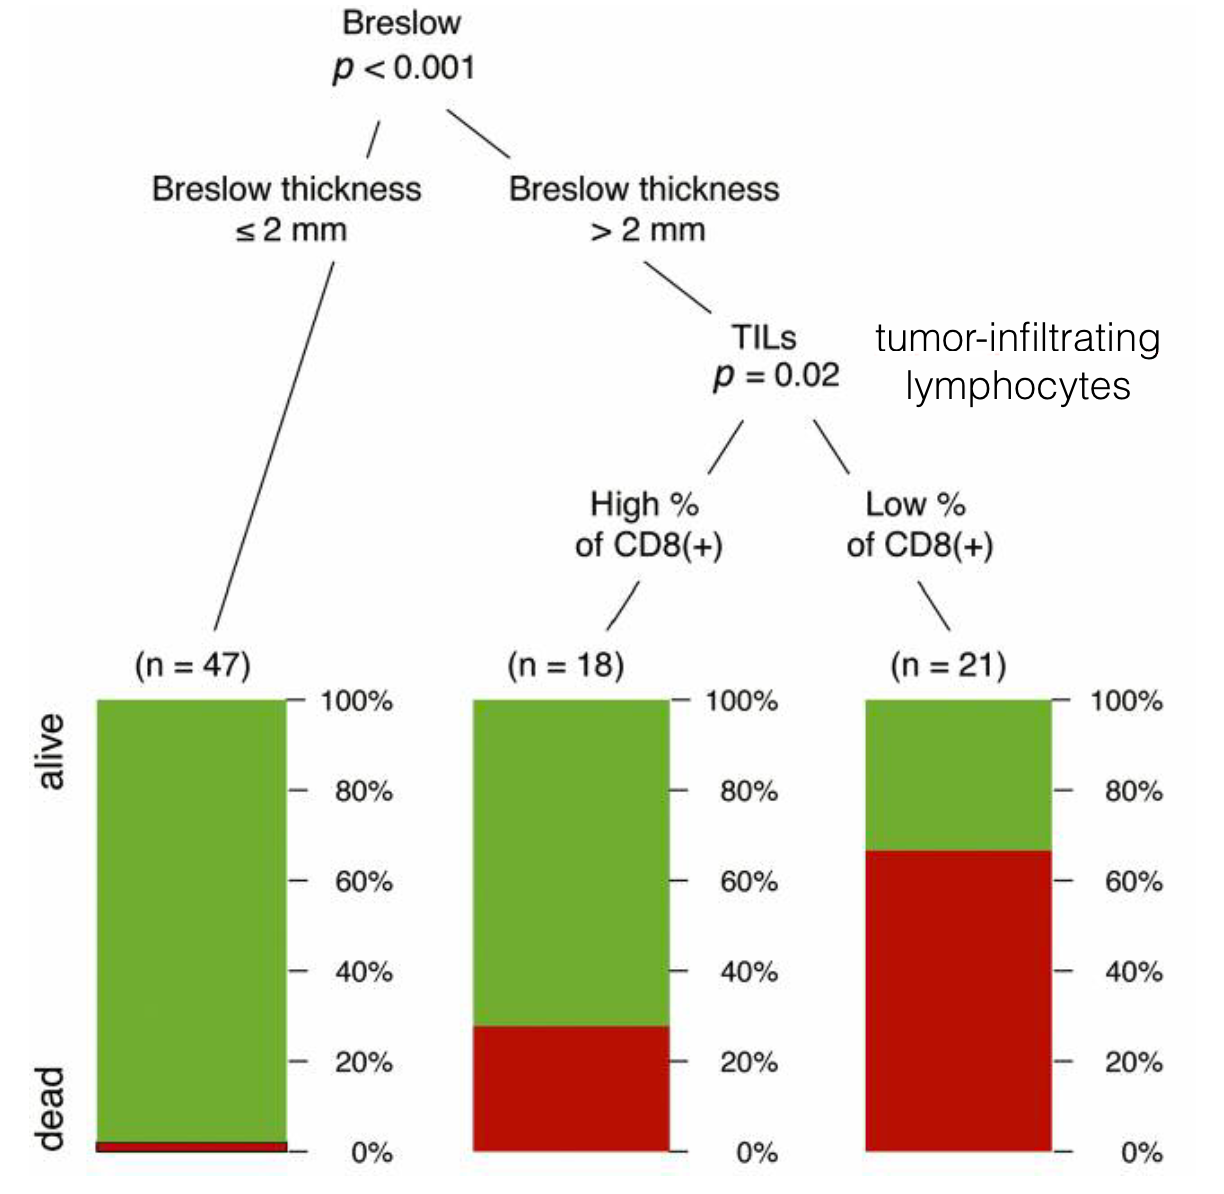
\includegraphics[width=0.5\linewidth]{figure/wbBILL8model} \end{center}

\hypertarget{model-visualization-exploration-and-explanation}{%
\subsection{Model visualization, exploration, and
explanation}\label{model-visualization-exploration-and-explanation}}

The lifecycle of a model can be divided, in general, in three different
phases: development (or building), deployment, and maintenance.

Model development is the phase in which one is looking for the best
available model. During this process, model exploration tools are
useful. Exploration involves evaluation of the fit of the model,
verification of the assumptions underlying the model (diagnostics), and
assessment of the predictive performance of the model (validation). In
our book we will focus on the visualization tools that can be useful in
model exploration. We will not, however, discuss visualization methods
for diagnostic purposes, as they are extensively discussed in many books
devoted to statistical modelling.

Model deployment is the phase in which a predictive model is adopted for
use. In this phase it is crucial that the users gain confidence in using
the model. It is worth noting that the users might not have been
involved in the model development. Moreover, they may only have got
access to the software implementing the model that may not provide any
insight in the details of the model structure. In this situation, model
explanation tools can help to understand the factors that influence
model predictions and to gain confidence in the model. The tools are one
of the main focu point of our book.

Finally, a deployed model requires maintenance. In this phase, one
monitors model's performance by, for instance, checking the validity of
predictions for different datasets. If issues are detected, model
explanation tools may be used to find the source of the problem and to
suggest a modification of the structure of the model.

\hypertarget{model-agnostic-vs.model-specific-approach}{%
\subsection{Model-agnostic vs.~model-specific
approach}\label{model-agnostic-vs.model-specific-approach}}

Some classes of models have been developed for a long period of time or
have attracted a lot of interest with an intensive research as a result.
Consequently, those classes of models are equipped with very good tools
for model exploration or visualisation. For example:

\begin{itemize}
\tightlist
\item
  There are many tools for diagnostics and evaluation of linear models.
  Model assumptions are formally defined (normality, linear structure,
  homogenous variance) and can be checked by using normality tests or
  plots (normal qq-plot), diagnostic plots, tests for model structure,
  tools for identification of outliers, etc.
\item
  For many more advanced models with an additive structure, like the
  proportional hazards model, there also many tools that can be used for
  checking model assumptions.
\item
  Random-forest model is equipped with the out-of-bag method of
  evaluation of performance and several tools for measuring variable
  importance \citep{R-randomForest}. Methods have been developed to
  extract information from the model structure about possible
  interactions \citep{R-randomForestExplainer}. Similar tools have been
  developed for other ensembles of trees, like xgboost models
  \citep{R-xgboostExplainer}.
\item
  Neural networks enjoy a large collection of dedicated
  model-explanation tools that use, for instance, the layer-wise
  relevance propagation technique \citep{BachLWRP}, or saliency maps
  technique \citep{SaliencyMaps}, or a mixed approach.
\end{itemize}

Of course, the list of model classes with dedicated collections of
model-explanation and/or diagnostics methods is much longer. This
variety of model-specific approaches does lead to issues, though. For
instance, one cannot easily compare explanations for two models with
different structures. Also, every time when a new architecture or a new
ensemble of models is proposed, one needs to look for new methods of
model exploration. Finally, for brand-new models no tools for model
explanation or diagnostics may be immedaitely available.

For these reasons, in our book we focus on model-agnostic techniques. In
particular, we prefer not to assume anything about the model structure,
as we may be dealing with a black-box model with an unclear structure.
In that case, the only operation that we may be able to perform is
evaluation of a model for a selected observation.

However, while we do not assume anything about the structure of the
model, we will assume that the model operates on \(p\)-dimensional
vectors and, for a single vector, it returns a single value which is a
real number. This assumption holds for a broad range of models for data
such as tabular data, images, text data, videos, etc. It may not be
suitable for, e.g., models with memory in which the model output does
not depend only on the model input {[}TOMASZ: NOT SURE WHICH MODELS ARE
MEANT HERE{]}.

Note that the techniques considered in the book may not be sufficient to
fully understand models in case \(p\) is large.

\hypertarget{code-snippets}{%
\subsection{Code snippets}\label{code-snippets}}

TODO: Here we should tell why we present examples for DALEX. And mention
that there are also other functions that can be used.

\hypertarget{the-structure-of-the-book}{%
\subsection{The structure of the book}\label{the-structure-of-the-book}}

Our book is split in two parts. In the part \emph{Instance-level
explainers}, we present techniques for exploration and explanation of
model predictions for a single observation. On the other hand, in the
part \emph{Global explainers}, we present techniques for exploration and
explanation of model's performance for an entire dataset. In each part,
every method is described in a separate section that has got the same
structure: * Subsection \emph{Introduction} explains the goal of and the
general idea behind the method. * Subsection \emph{The Algorithm} shows
mathematical or computational details related to the method. This
subsection can be skipped if you are not interested in the details. *
Subsection \emph{Example} shows an exemplary application of the method
with discussion of results. * Subsection \emph{Pros and Cons} summarizes
the advantages and disadvantages of the method. It also provides some
guideance regarding when to use the method. * Subsection \emph{Code
snippets} shows the implementation of the method in R and Python. This
subsection can be skipped if you are not interested in the
implementation.

TO DO: A SHORT REVIEW OF THE CONTENTS OF VARIOUS CHAPTERS

Finally, we would like to signal that, \textbf{in this book, we do show}

\begin{itemize}
\tightlist
\item
  how to determine features that affect model prediction for a single
  observation. In particular, we present the theory and examples of
  methods that can be used to explain prediction like break down plots,
  ceteris paribus profiles, local-model approximations, or Shapley
  values.
\item
  techniques to examine fully-trained machine-learning models as a
  whole. In particular, we review the theory and examples of methods
  that can be used to explain model performance globally, like
  partial-dependency plots, variable-importance plots, and others.
\item
  charts that can be used to present key information in a quick way.
\item
  tools and methods for model comparison.
\item
  code snippets for R and Python that explain how to use the described
  methods.
\end{itemize}

On the other hand, \textbf{in this book, we do not focus on}

\begin{itemize}
\tightlist
\item
  any specific model. The presented techniques are model agnostic and do
  not make any assumptions related to model structure.
\item
  data exploration. There are very good books on this topic, like R for
  Data Science \url{http://r4ds.had.co.nz/} or TODO
\item
  the process of model building. There are also very good books on this
  topic, see An Introduction to Statistical Learning by Gareth James,
  Daniela Witten, Trevor Hastie and Robert Tibshirani
  \url{http://www-bcf.usc.edu/~gareth/ISL/} or TODO
\item
  any particular tools for model building. These are discussed, for
  instance, in Applied Predictive Modeling By Max Kuhn and Kjell Johnson
  \url{http://appliedpredictivemodeling.com/}
\end{itemize}

\hypertarget{thanksto}{%
\subsection{Acknowledgements}\label{thanksto}}

Przemek's work on interpretability has started during research trips
within the RENOIR project (691152 - H2020/2016-2019). So he would like
to thank prof. Janusz Holyst for the chance to take part in this
project.

Przemek would also like thank prof. Chris Drake for her hospitality.
This book would have never been created without perfect conditions that
Przemek found at Chris' house in Woodland.

This book has been prepared by using the \textbf{bookdown} package
\citep{R-bookdown}, created thanks to the amazing work of Yihui Xie.

\hypertarget{DataSetsIntro}{%
\section{Data Sets}\label{DataSetsIntro}}

We illustrate the techniques presented in this book by using three
datasets:

\begin{itemize}
\tightlist
\item
  \emph{Sinking of the RMS Titanic}
\item
  \emph{Apartment prices}
\item
  \emph{Hire or Fire}
\end{itemize}

The first dataset will be used to illustrate the application of the
techniques in the case of a predictive model for a binary dependent
variable. The second one will provide an example for models for a
continuous variable. Finally, the third dataset will be used for
illustration of models for a categorical dependent variable.

In this chapter, we provide a short description of each of the datasets,
together with results of exploratory analyses. We also introduce models
that will be used for illustration purposes in subsequent chapters.

\hypertarget{TitanicDataset}{%
\subsection{Sinking of the RMS Titanic}\label{TitanicDataset}}

\begin{figure}
\centering
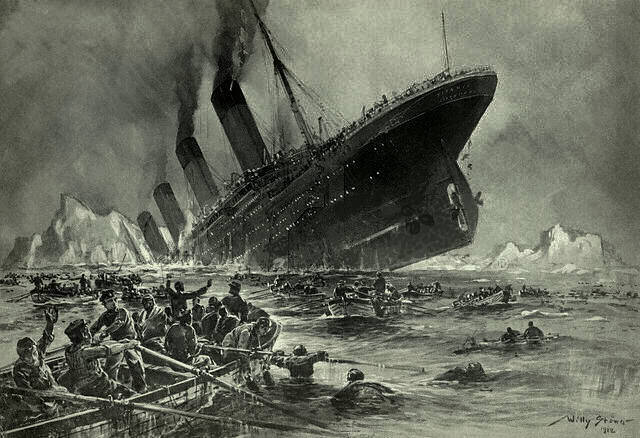
\includegraphics{figure/Titanic.jpg}
\caption{Titanic sinking by Willy Stöwer}
\end{figure}

Sinking of the RMS Titanic is one of the deadliest maritime disasters in
history (during peacetime). Over 1500 people died as a consequence of
collision with an iceberg. Projects like \emph{Encyclopedia titanica}
\texttt{https://www.encyclopedia-titanica.org/} are a source of rich and
precise data about Titanic's passengers. The data are available in a
dataset included in the \texttt{stablelearner} package. The dataset,
after some data cleaning and variable transformations, is also avaliable
in the \texttt{DALEX} package. In particular, the `titanic' data frame
contains 2207 observations (for 1317 passengers and 890 crew members)
and nine variables:

\begin{itemize}
\tightlist
\item
  \emph{gender}, person's (passenger's or crew member's) gender, a
  factor (categorical variable) with two levels (categories)
\item
  \emph{age}, person's age in years, a numerical variable; for adults,
  the age is given in (integer) years; for children younger than one
  year, the age is given as \(x/12\), where \(x\) is the number of
  months of child's age
\item
  \emph{class}, the class in which the passenger travelled, or the duty
  class of a crew member; a factor with seven levels
\item
  \emph{embarked}, the harbor in which the person embarked on the ship,
  a factor with four levels
\item
  \emph{country}, person's home country, a factor with 48 levels
\item
  \emph{fare}, the price of the ticket (only available for passengers; 0
  for crew members), a numerical variable
\item
  \emph{sibsp}, the number of siblings/spouses aboard the ship, a
  numerical variable
\item
  \emph{parch}, the number of parents/children aboard the ship, a
  numerical variable
\item
  \emph{survived}, a factor with two levels indicating whether the
  person survived or not
\end{itemize}

Models considered for this dataset will use \emph{survived} as the
(binary) dependent variable.

\begin{Shaded}
\begin{Highlighting}[]
\KeywordTok{library}\NormalTok{(}\StringTok{"DALEX"}\NormalTok{)}
\KeywordTok{head}\NormalTok{(titanic, }\DecValTok{2}\NormalTok{)}
\end{Highlighting}
\end{Shaded}

\begin{verbatim}
##   gender age class    embarked       country  fare sibsp parch survived
## 1   male  42   3rd Southampton United States  7.11     0     0       no
## 2   male  13   3rd Southampton United States 20.05     0     2       no
\end{verbatim}

\begin{Shaded}
\begin{Highlighting}[]
\KeywordTok{str}\NormalTok{(titanic)}
\end{Highlighting}
\end{Shaded}

\begin{verbatim}
## 'data.frame':    2207 obs. of  9 variables:
##  $ gender  : Factor w/ 2 levels "female","male": 2 2 2 1 1 2 2 1 2 2 ...
##  $ age     : num  42 13 16 39 16 25 30 28 27 20 ...
##  $ class   : Factor w/ 7 levels "1st","2nd","3rd",..: 3 3 3 3 3 3 2 2 3 3 ...
##  $ embarked: Factor w/ 4 levels "Belfast","Cherbourg",..: 4 4 4 4 4 4 2 2 2 4 ...
##  $ country : Factor w/ 48 levels "Argentina","Australia",..: 44 44 44 15 30 44 17 17 26 16 ...
##  $ fare    : num  7.11 20.05 20.05 20.05 7.13 ...
##  $ sibsp   : num  0 0 1 1 0 0 1 1 0 0 ...
##  $ parch   : num  0 2 1 1 0 0 0 0 0 0 ...
##  $ survived: Factor w/ 2 levels "no","yes": 1 1 1 2 2 2 1 2 2 2 ...
\end{verbatim}

\begin{Shaded}
\begin{Highlighting}[]
\KeywordTok{levels}\NormalTok{(titanic}\OperatorTok{$}\NormalTok{class)}
\end{Highlighting}
\end{Shaded}

\begin{verbatim}
## [1] "1st"              "2nd"              "3rd"             
## [4] "deck crew"        "engineering crew" "restaurant staff"
## [7] "victualling crew"
\end{verbatim}

\begin{Shaded}
\begin{Highlighting}[]
\KeywordTok{levels}\NormalTok{(titanic}\OperatorTok{$}\NormalTok{embarked)}
\end{Highlighting}
\end{Shaded}

\begin{verbatim}
## [1] "Belfast"     "Cherbourg"   "Queenstown"  "Southampton"
\end{verbatim}

\hypertarget{data-exploration}{%
\subsubsection{Data exploration}\label{data-exploration}}

It is always advisable to explore data before modelling. However, as
this book is focused on model exploration, we will limit the data
exploration part.

Before exploring the data, we first do some pre-processing. In
particular, the value of variables \emph{age}, \emph{country},
\emph{sibsp}, \emph{parch}, and \emph{fare} is missing for a limited
number of observations (2, 81, 10, 10, and 26, respectively). Analyzing
data with missing values is a topic on its own (Little and Rubin 1987;
Schafer 1997; Molenberghs and Kenward 2007). An often-used approach is
to impute the missing values. Toward this end, multiple imputation
should be considered (Schafer 1997; Molenberghs and Kenward 2007; van
Buuren 2012). However, given the limited number of missing values and
the intended illustrative use of the dataset, we will limit ourselves
to, admittedly inferior, single imputation. In particular, we replace
the missing \emph{age} values by the mean of the observed ones, i.e.,
30. Missing \emph{country} will be coded by ``X''. For \emph{sibsp} and
\emph{parch}, we replace the missing values by the most frequently
observed value, i.e., 0. Finally, for \emph{fare}, we use the value of
0.

{[}TOMASZ: FOR FARE, ONE COULD USE THE MEAN OF OBSERVED VALUES, AS FOR
AGE. TAKING 0 CORRESPONDS TO ``crew''. PBI there are 7, 14, 5 missing
values in the 1st/2nd/3rd class. Fare differs among classes, so maybe it
should be a class average?{]}

\begin{Shaded}
\begin{Highlighting}[]
\CommentTok{# missing country is replaced by "X"}
\NormalTok{titanic}\OperatorTok{$}\NormalTok{country[}\KeywordTok{is.na}\NormalTok{(titanic}\OperatorTok{$}\NormalTok{country)] =}\StringTok{ "X"}
\CommentTok{# missing age is replaced by average (30)}
\NormalTok{titanic}\OperatorTok{$}\NormalTok{age[}\KeywordTok{is.na}\NormalTok{(titanic}\OperatorTok{$}\NormalTok{age)] =}\StringTok{ }\DecValTok{30}
\CommentTok{# missing sibsp, parch are replaced by 0}
\NormalTok{titanic}\OperatorTok{$}\NormalTok{sibsp[}\KeywordTok{is.na}\NormalTok{(titanic}\OperatorTok{$}\NormalTok{sibsp)] =}\StringTok{ }\DecValTok{0}
\NormalTok{titanic}\OperatorTok{$}\NormalTok{parch[}\KeywordTok{is.na}\NormalTok{(titanic}\OperatorTok{$}\NormalTok{parch)] =}\StringTok{ }\DecValTok{0}
\CommentTok{# missing fare is replaced by class average}
\KeywordTok{tapply}\NormalTok{(titanic}\OperatorTok{$}\NormalTok{fare, titanic}\OperatorTok{$}\NormalTok{class, mean, }\DataTypeTok{na.rm =} \OtherTok{TRUE}\NormalTok{)}
\end{Highlighting}
\end{Shaded}

\begin{verbatim}
##              1st              2nd              3rd        deck crew 
##         89.01734         21.50308         12.92786          0.00000 
## engineering crew restaurant staff victualling crew 
##          0.00000          0.00000          0.00000
\end{verbatim}

\begin{Shaded}
\begin{Highlighting}[]
\NormalTok{titanic}\OperatorTok{$}\NormalTok{fare[}\KeywordTok{is.na}\NormalTok{(titanic}\OperatorTok{$}\NormalTok{fare) }\OperatorTok{&}\StringTok{ }\NormalTok{titanic}\OperatorTok{$}\NormalTok{class }\OperatorTok{==}\StringTok{ "1st"}\NormalTok{] =}\StringTok{ }\DecValTok{89}
\NormalTok{titanic}\OperatorTok{$}\NormalTok{fare[}\KeywordTok{is.na}\NormalTok{(titanic}\OperatorTok{$}\NormalTok{fare) }\OperatorTok{&}\StringTok{ }\NormalTok{titanic}\OperatorTok{$}\NormalTok{class }\OperatorTok{==}\StringTok{ "2nd"}\NormalTok{] =}\StringTok{ }\DecValTok{22}
\NormalTok{titanic}\OperatorTok{$}\NormalTok{fare[}\KeywordTok{is.na}\NormalTok{(titanic}\OperatorTok{$}\NormalTok{fare) }\OperatorTok{&}\StringTok{ }\NormalTok{titanic}\OperatorTok{$}\NormalTok{class }\OperatorTok{==}\StringTok{ "3rd"}\NormalTok{] =}\StringTok{ }\DecValTok{13}
\end{Highlighting}
\end{Shaded}

After imputing the missing values, we investigate the association
between survival status and the other variables. Figures XXX-XXX present
graphically the proportion non- and survivors for different levels of
the other variables. The height of the bars (on the y-axis) reflects the
marginal distribution (proportions) of the observed levels of the
variable. On the other hand, the width of the bars (on the x-axis)
provides the information about the proportion of non- and survivors.
Note that, to construct the graphs for \emph{age} and \emph{fare}, we
categorized the range of the observed values.

{[}TOMASZ: CHANGE THE ORDER, AS SUGGESTED IN THE R CODE. LABEL THE
HORIZONTAL ``SURVIVAL'' AXIS WITH PROPORTIONS. IMPROVE LABELING OF THE
Y-AXIS. {]}

Figures @ref(fig:titanic\_exploration\_gender) and
@ref(fig:titanic\_exploration\_age) indicate that the proportion of
survivors was larger for females and children below 5 years of age. This
is most likely the result of the ``women and children first'' principle
that is often evoked in situations that require evacuation of persons
whose life is in danger. The principle can, perhaps, partially explain
the trend seen in Figures @ref(fig:titanic\_exploration\_parch) and
@ref(fig:titanic\_exploration\_sibsp), i.e., a higher proportion of
survivors among those with 1-3 parents/children and 1-2 siblings/spouses
aboard. Figure @ref(fig:titanic\_exploration\_class) indicates that
passengers travelling in the first and second class had a higher chance
of survival, perhaps due to the proximity of the location of their
cabins to the deck. Interestingly, the proportion of survivors among
crew deck was similar to the proportion of the first-class passengers.
Figure @ref(fig:titanic\_exploration\_fare) shows that the proportion of
survivors increased with the fare, which is consistent with the fact
that the proportion was higher for passengers travelling in the first
and second class. Finally, Figures
@ref(fig:titanic\_exploration\_embarked) and
\ref(fig:titanic\_exploration\_country) do not suggest any noteworthy
trends.

\textbackslash{}begin\{figure\}

\{\centering 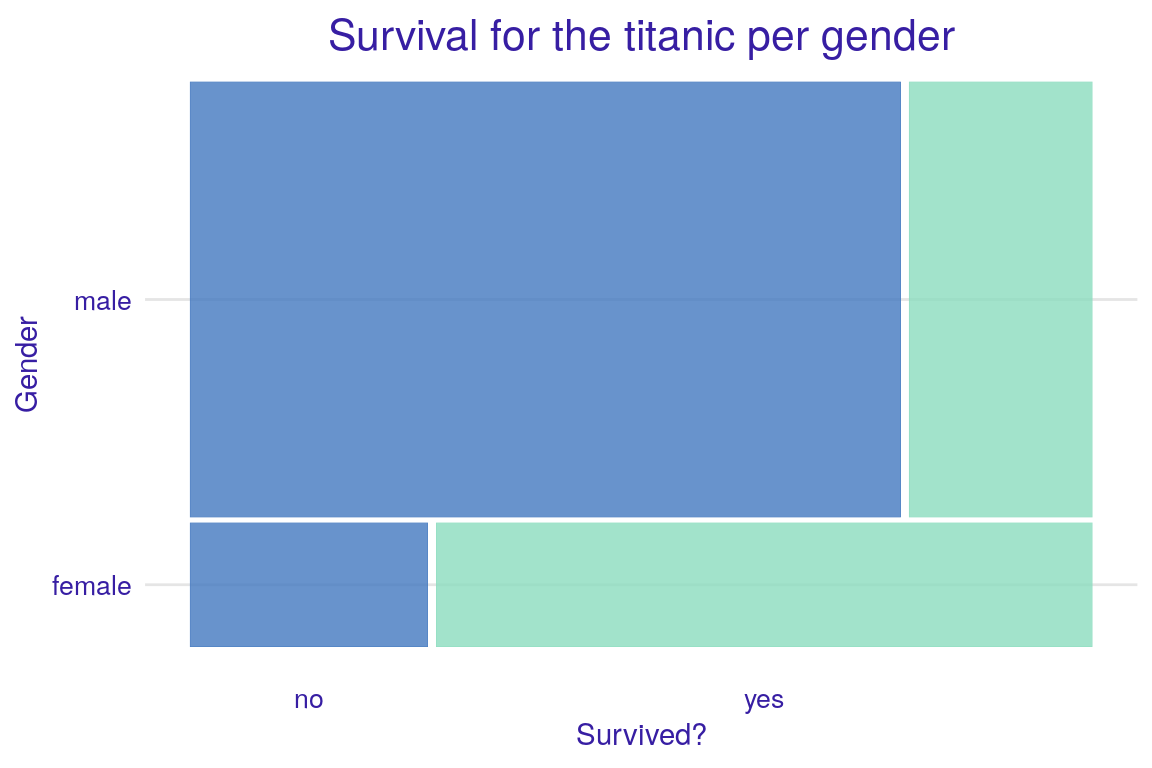
\includegraphics[width=0.7\linewidth]{PM_VEE_files/figure-latex/titanic_exploration_gender-1}

\}

\textbackslash{}caption\{(fig:titanic\_exploration\_gender) Survival in
different genders for the titanic
data.\}(\#fig:titanic\_exploration\_gender)
\textbackslash{}end\{figure\}

\textbackslash{}begin\{figure\}

\{\centering 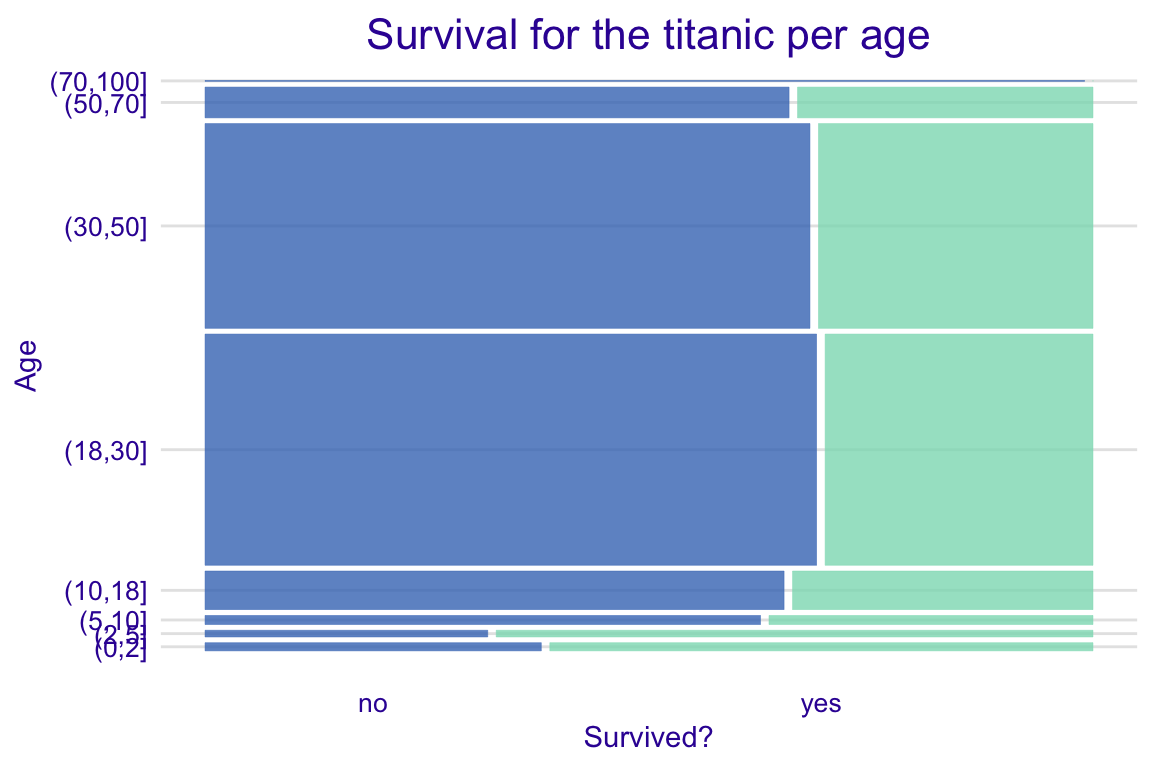
\includegraphics[width=0.7\linewidth]{PM_VEE_files/figure-latex/titanic_exploration_age-1}

\}

\textbackslash{}caption\{(fig:titanic\_exploration\_age) Survival in
different age groups for the titanic
data.\}(\#fig:titanic\_exploration\_age) \textbackslash{}end\{figure\}

\textbackslash{}begin\{figure\}

\{\centering 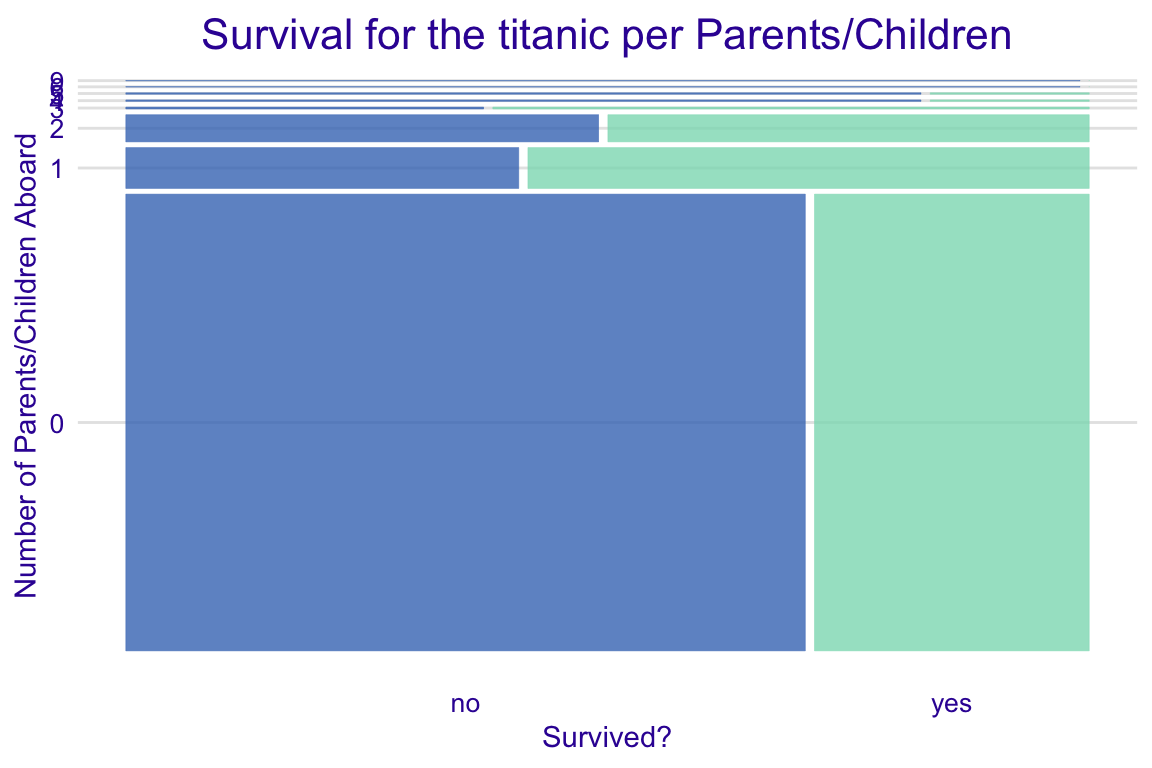
\includegraphics[width=0.7\linewidth]{PM_VEE_files/figure-latex/titanic_exploration_parch-1}

\}

\textbackslash{}caption\{(fig:titanic\_exploration\_parch) Survival in
different numbers of parents/children for the titanic
data.\}(\#fig:titanic\_exploration\_parch) \textbackslash{}end\{figure\}

\textbackslash{}begin\{figure\}

\{\centering 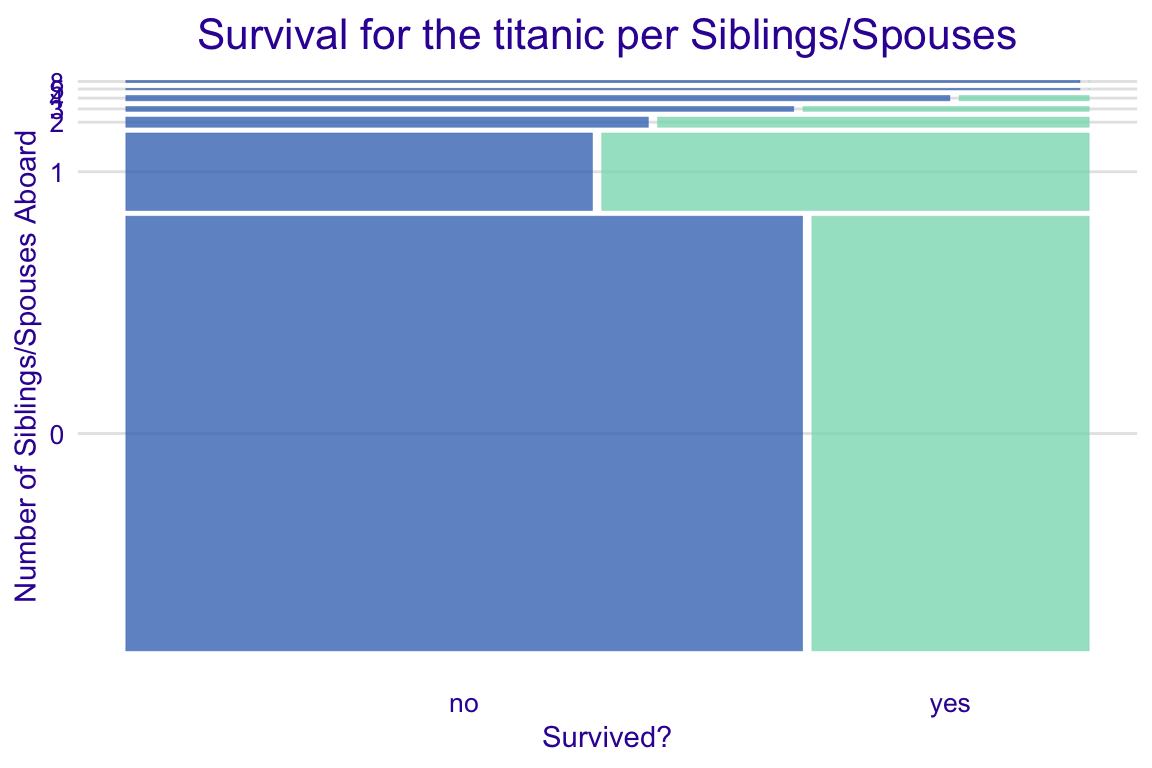
\includegraphics[width=0.7\linewidth]{PM_VEE_files/figure-latex/titanic_exploration_sibsp-1}

\}

\textbackslash{}caption\{(fig:titanic\_exploration\_sibsp) Survival in
different numbers of siblings/spouses for the titanic
data.\}(\#fig:titanic\_exploration\_sibsp) \textbackslash{}end\{figure\}

\textbackslash{}begin\{figure\}

\{\centering 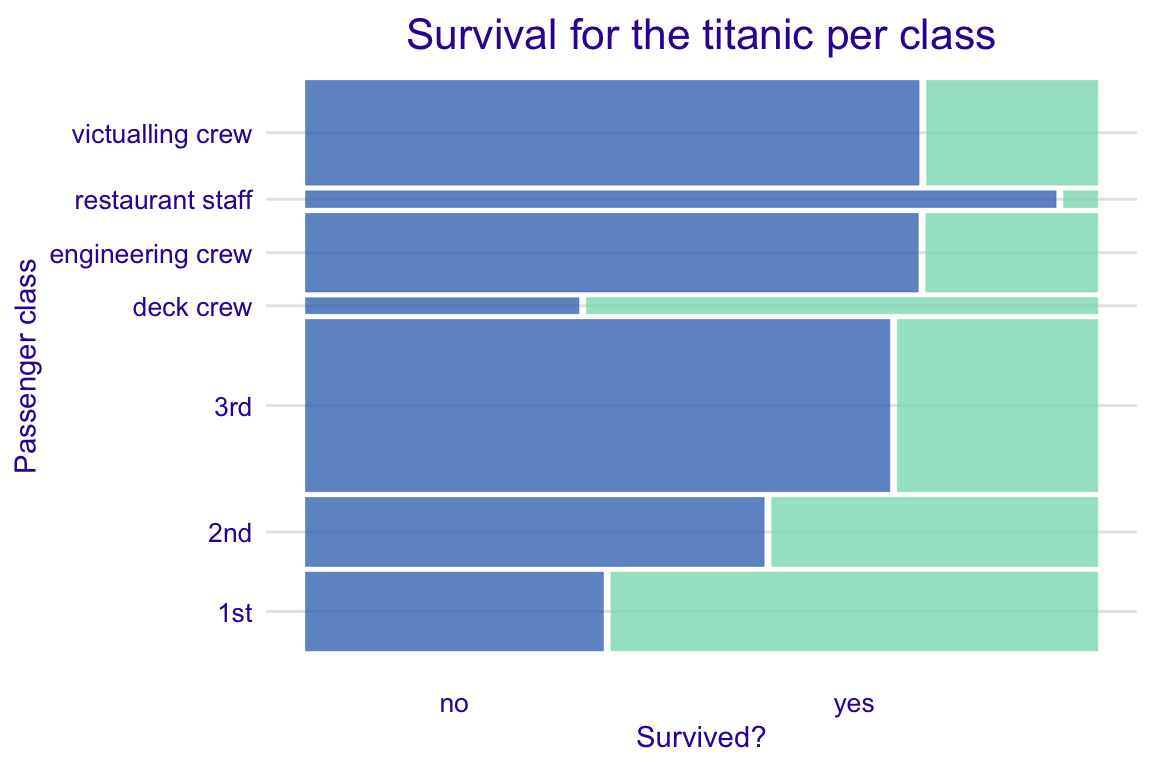
\includegraphics[width=0.7\linewidth]{PM_VEE_files/figure-latex/titanic_exploration_class-1}

\}

\textbackslash{}caption\{(fig:titanic\_exploration\_class) Survival for
different classes in the titanic
data.\}(\#fig:titanic\_exploration\_class) \textbackslash{}end\{figure\}

\begin{figure}
\centering
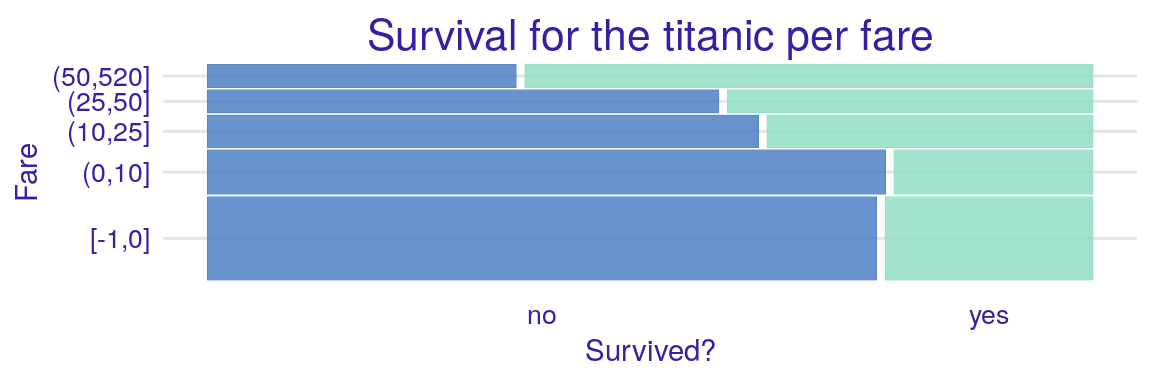
\includegraphics{PM_VEE_files/figure-latex/titanic_exploration_fare-1.pdf}
\caption{(\#fig:titanic\_exploration\_fare)(fig:titanic\_exploration\_fare)
Survival as a function of fare in the titanic data.}
\end{figure}

\begin{figure}
\centering
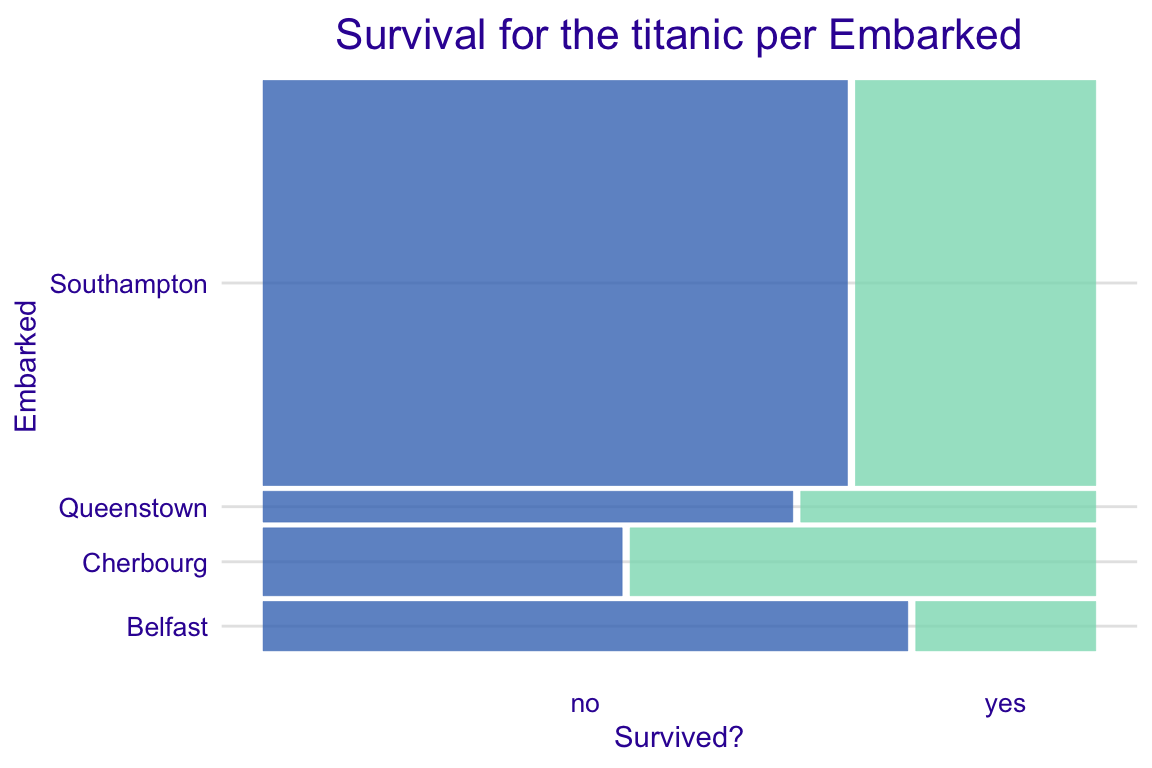
\includegraphics{PM_VEE_files/figure-latex/titanic_exploration_embarked-1.pdf}
\caption{(\#fig:titanic\_exploration\_embarked)(fig:titanic\_exploration\_embarked)
Survival for different port of embarking in the titanic data.}
\end{figure}

\begin{figure}
\centering
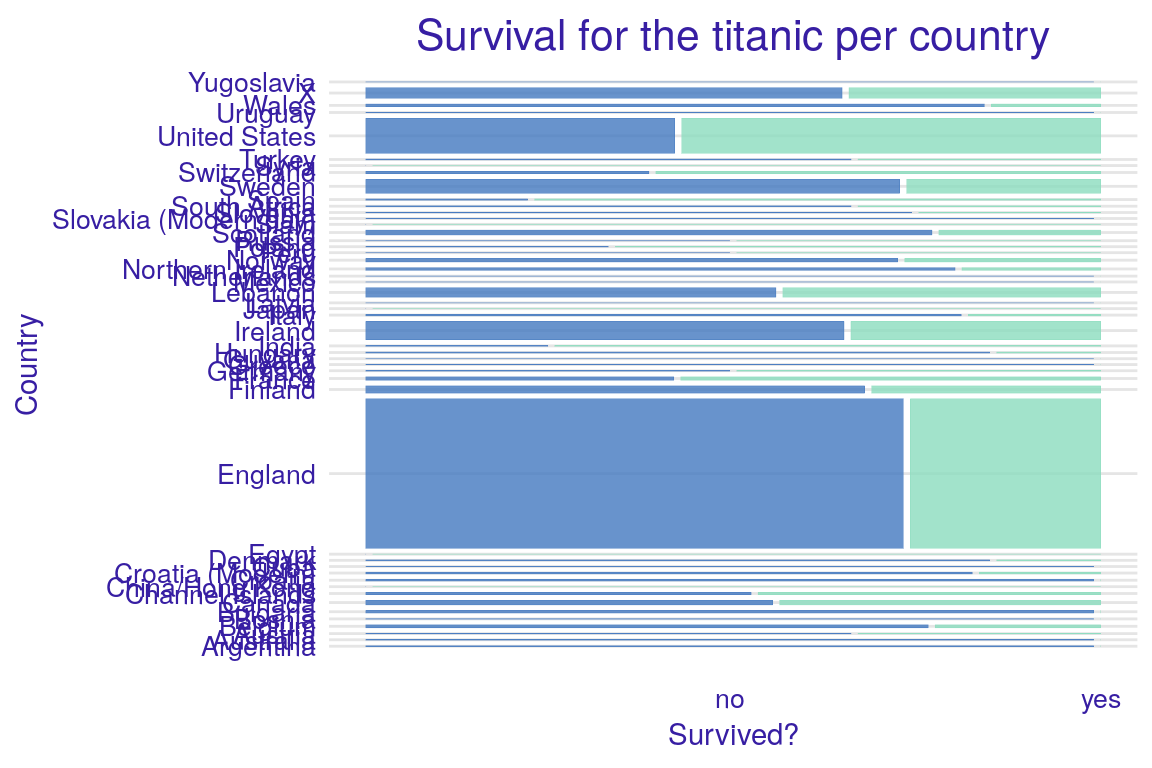
\includegraphics{PM_VEE_files/figure-latex/titanic_exploration_country-1.pdf}
\caption{(\#fig:titanic\_exploration\_country)(fig:titanic\_exploration\_country)
Survival for different countries in the titanic data.}
\end{figure}

\hypertarget{model_titanic_lmr}{%
\subsubsection{Logistic regression}\label{model_titanic_lmr}}

The dependent variable of interest, \emph{survival}, is binary. Thus, a
natural choice to build a predictive model is logistic regression. We do
not consider country as an explanatory variable. As there is no reason
to expect a linear relationship between age and odds of survival, we use
linear tail-restricted cubic splines, available in the \texttt{rcs()}
function of the \texttt{rms} package \citep{rms}, to model the effect of
age. {[}TOMASZ: IS THERE A REASON TO ASSUME A LINEAR EFFECT OF FARE?
PBI: it's not linear but something modeled with slines{]} The results of
the model are stored in model-object \texttt{titanic\_lmr\_v6}, which
will be used in subsequent chapters.

\begin{Shaded}
\begin{Highlighting}[]
\KeywordTok{library}\NormalTok{(}\StringTok{"rms"}\NormalTok{)}
\NormalTok{titanic_lmr_v6 <-}\StringTok{ }\KeywordTok{lrm}\NormalTok{(survived }\OperatorTok{==}\StringTok{ "yes"} \OperatorTok{~}\StringTok{ }\NormalTok{gender }\OperatorTok{+}\StringTok{ }\KeywordTok{rcs}\NormalTok{(age) }\OperatorTok{+}\StringTok{ }\NormalTok{class }\OperatorTok{+}\StringTok{ }\NormalTok{sibsp }\OperatorTok{+}
\StringTok{                   }\NormalTok{parch }\OperatorTok{+}\StringTok{ }\NormalTok{fare }\OperatorTok{+}\StringTok{ }\NormalTok{embarked, titanic)}
\NormalTok{titanic_lmr_v6}
\end{Highlighting}
\end{Shaded}

\begin{verbatim}
## Logistic Regression Model
##  
##  lrm(formula = survived == "yes" ~ gender + rcs(age) + class + 
##      sibsp + parch + fare + embarked, data = titanic)
##  
##                         Model Likelihood     Discrimination    Rank Discrim.    
##                            Ratio Test           Indexes           Indexes       
##  Obs           2207    LR chi2     752.06    R2       0.404    C       0.817    
##   FALSE        1496    d.f.            17    g        1.647    Dxy     0.635    
##   TRUE          711    Pr(> chi2) <0.0001    gr       5.191    gamma   0.636    
##  max |deriv| 0.0001                          gp       0.282    tau-a   0.277    
##                                              Brier    0.146                     
##  
##                         Coef    S.E.   Wald Z Pr(>|Z|)
##  Intercept               4.5746 0.5480   8.35 <0.0001 
##  gender=male            -2.7687 0.1586 -17.45 <0.0001 
##  age                    -0.1180 0.0221  -5.35 <0.0001 
##  age'                    0.6313 0.1628   3.88 0.0001  
##  age''                  -2.6583 0.7840  -3.39 0.0007  
##  age'''                  2.8977 1.0130   2.86 0.0042  
##  class=2nd              -1.1390 0.2501  -4.56 <0.0001 
##  class=3rd              -2.0627 0.2490  -8.28 <0.0001 
##  class=deck crew         1.0672 0.3498   3.05 0.0023  
##  class=engineering crew -0.9702 0.2648  -3.66 0.0002  
##  class=restaurant staff -3.1712 0.6583  -4.82 <0.0001 
##  class=victualling crew -1.0877 0.2596  -4.19 <0.0001 
##  sibsp                  -0.4504 0.1006  -4.48 <0.0001 
##  parch                  -0.0871 0.0987  -0.88 0.3776  
##  fare                    0.0014 0.0020   0.70 0.4842  
##  embarked=Cherbourg      0.7881 0.2836   2.78 0.0055  
##  embarked=Queenstown     0.2745 0.3409   0.80 0.4208  
##  embarked=Southampton    0.2343 0.2119   1.11 0.2689  
## 
\end{verbatim}

\hypertarget{model_titanic_rf}{%
\subsubsection{Random forest}\label{model_titanic_rf}}

As an alternative to a logistic regression model, we consider a random
forest model. Random forest is known for good predictive performance, is
able to grasp low-level variable interactions, and is quite stable
{[}TOMASZ: REFERENCE?{]}. To fit the model, we apply the
\texttt{randomForest()} function, with default settings, from the
package with the same name \citep{randomForestRNews}.

In the first instance, we fit a model with the same set of explanatory
variables as the logistic regression model. The results of the model are
stored in model-object \texttt{titanic\_rf\_v6}.

\begin{Shaded}
\begin{Highlighting}[]
\KeywordTok{library}\NormalTok{(}\StringTok{"randomForest"}\NormalTok{)}
\NormalTok{titanic_rf_v6 <-}\StringTok{ }\KeywordTok{randomForest}\NormalTok{(survived }\OperatorTok{~}\StringTok{ }\NormalTok{class }\OperatorTok{+}\StringTok{ }\NormalTok{gender }\OperatorTok{+}\StringTok{ }\NormalTok{age }\OperatorTok{+}\StringTok{ }\NormalTok{sibsp }\OperatorTok{+}\StringTok{ }\NormalTok{parch }\OperatorTok{+}\StringTok{ }\NormalTok{fare }\OperatorTok{+}\StringTok{ }\NormalTok{embarked, }
                           \DataTypeTok{data =}\NormalTok{ titanic)}
\NormalTok{titanic_rf_v6}
\end{Highlighting}
\end{Shaded}

\begin{verbatim}
## 
## Call:
##  randomForest(formula = survived ~ class + gender + age + sibsp +      parch + fare + embarked, data = titanic) 
##                Type of random forest: classification
##                      Number of trees: 500
## No. of variables tried at each split: 2
## 
##         OOB estimate of  error rate: 18.35%
## Confusion matrix:
##       no yes class.error
## no  1401  95  0.06350267
## yes  310 401  0.43600563
\end{verbatim}

For comparison purposes, we also consider a model with only three
explanatory variables: \emph{class}, \emph{gender}, and \emph{age}. The
results of the model are stored in model-object
\texttt{titanic\_rf\_v3}.

\begin{Shaded}
\begin{Highlighting}[]
\NormalTok{titanic_rf_v3 <-}\StringTok{ }\KeywordTok{randomForest}\NormalTok{(survived }\OperatorTok{~}\StringTok{ }\NormalTok{class }\OperatorTok{+}\StringTok{ }\NormalTok{gender }\OperatorTok{+}\StringTok{ }\NormalTok{age, }\DataTypeTok{data =}\NormalTok{ titanic)}
\NormalTok{titanic_rf_v3}
\end{Highlighting}
\end{Shaded}

\begin{verbatim}
## 
## Call:
##  randomForest(formula = survived ~ class + gender + age, data = titanic) 
##                Type of random forest: classification
##                      Number of trees: 500
## No. of variables tried at each split: 1
## 
##         OOB estimate of  error rate: 20.75%
## Confusion matrix:
##       no yes class.error
## no  1358 138  0.09224599
## yes  320 391  0.45007032
\end{verbatim}

\hypertarget{gradient-boosting}{%
\subsubsection{Gradient boosting}\label{gradient-boosting}}

Finally, we consider the gradient-boosting model. The model is known for
being able to grasp deep interactions between variables. {[}TOMASZ: WHAT
ARE ``DEEP INTERACTIONS''? REFERENCE?{]} We use the same set of
explanatory variables as for the logistic regression model. To fit the
gradient-boosting model, we use the function \texttt{gbm()} from the
\texttt{gbm} package \citep{gbm}. The results of the model are stored in
model-object \texttt{titanic\_gbm\_v6}.

\begin{Shaded}
\begin{Highlighting}[]
\KeywordTok{set.seed}\NormalTok{(}\DecValTok{1313}\NormalTok{)}

\KeywordTok{library}\NormalTok{(}\StringTok{"gbm"}\NormalTok{)}
\NormalTok{titanic_gbm_v6 <-}\StringTok{ }\KeywordTok{gbm}\NormalTok{(survived }\OperatorTok{==}\StringTok{ "yes"} \OperatorTok{~}\StringTok{ }\NormalTok{class }\OperatorTok{+}\StringTok{ }\NormalTok{gender }\OperatorTok{+}\StringTok{ }\NormalTok{age }\OperatorTok{+}\StringTok{ }\NormalTok{sibsp }\OperatorTok{+}\StringTok{ }\NormalTok{parch }\OperatorTok{+}\StringTok{ }\NormalTok{fare }\OperatorTok{+}\StringTok{ }\NormalTok{embarked, }
                      \DataTypeTok{data =}\NormalTok{ titanic, }\DataTypeTok{n.trees =} \DecValTok{15000}\NormalTok{)}
\end{Highlighting}
\end{Shaded}

\begin{verbatim}
## Distribution not specified, assuming bernoulli ...
\end{verbatim}

\begin{Shaded}
\begin{Highlighting}[]
\NormalTok{titanic_gbm_v6}
\end{Highlighting}
\end{Shaded}

\begin{verbatim}
## gbm(formula = survived == "yes" ~ class + gender + age + sibsp + 
##     parch + fare + embarked, data = titanic, n.trees = 15000)
## A gradient boosted model with bernoulli loss function.
## 15000 iterations were performed.
## There were 7 predictors of which 7 had non-zero influence.
\end{verbatim}

\hypertarget{predictions_titanic}{%
\subsubsection{Model predictions}\label{predictions_titanic}}

Let us now compare predictions that are obtained from the three
different models. In particular, we will compute the predicted
probability of survival for an 8-year-old boy who embarked in Belfast
and travelled in the 2nd class with no parents nor siblings with a
ticket costing 72 pounds. First, we create a data frame \texttt{henry}
that contains the data describing the passenger.

\begin{Shaded}
\begin{Highlighting}[]
\NormalTok{henry <-}\StringTok{ }\KeywordTok{data.frame}\NormalTok{(}
            \DataTypeTok{class =} \KeywordTok{factor}\NormalTok{(}\StringTok{"2nd"}\NormalTok{, }\DataTypeTok{levels =} \KeywordTok{c}\NormalTok{(}\StringTok{"1st"}\NormalTok{, }\StringTok{"2nd"}\NormalTok{, }\StringTok{"3rd"}\NormalTok{, }\StringTok{"deck crew"}\NormalTok{, }\StringTok{"engineering crew"}\NormalTok{, }\StringTok{"restaurant staff"}\NormalTok{, }\StringTok{"victualling crew"}\NormalTok{)),}
            \DataTypeTok{gender =} \KeywordTok{factor}\NormalTok{(}\StringTok{"male"}\NormalTok{, }\DataTypeTok{levels =} \KeywordTok{c}\NormalTok{(}\StringTok{"female"}\NormalTok{, }\StringTok{"male"}\NormalTok{)),}
            \DataTypeTok{age =} \DecValTok{8}\NormalTok{,}
            \DataTypeTok{sibsp =} \DecValTok{0}\NormalTok{,}
            \DataTypeTok{parch =} \DecValTok{0}\NormalTok{,}
            \DataTypeTok{fare =} \DecValTok{72}\NormalTok{,}
            \DataTypeTok{embarked =} \KeywordTok{factor}\NormalTok{(}\StringTok{"Belfast"}\NormalTok{, }\DataTypeTok{levels =} \KeywordTok{c}\NormalTok{(}\StringTok{"Belfast"}\NormalTok{,}\StringTok{"Cherbourg"}\NormalTok{,}\StringTok{"Queenstown"}\NormalTok{,}\StringTok{"Southampton"}\NormalTok{))}
\NormalTok{)}
\end{Highlighting}
\end{Shaded}

Subsequently, we use the generic function \texttt{predict()} to get the
predicted probability of survival for the logistic regression model.

\begin{Shaded}
\begin{Highlighting}[]
\NormalTok{(}\DataTypeTok{pred_lmr =} \KeywordTok{predict}\NormalTok{(titanic_lmr_v6, henry, }\DataTypeTok{type =} \StringTok{"fitted"}\NormalTok{))}
\end{Highlighting}
\end{Shaded}

\begin{verbatim}
##         1 
## 0.4556319
\end{verbatim}

The predicted probability is equal to 0.46.

We do the same for the random forest and gradient boosting models.

\begin{Shaded}
\begin{Highlighting}[]
\NormalTok{(}\DataTypeTok{pred_rf =} \KeywordTok{predict}\NormalTok{(titanic_rf_v6, henry, }\DataTypeTok{type =} \StringTok{"prob"}\NormalTok{))}
\end{Highlighting}
\end{Shaded}

\begin{verbatim}
##      no   yes
## 1 0.642 0.358
## attr(,"class")
## [1] "matrix" "votes"
\end{verbatim}

\begin{Shaded}
\begin{Highlighting}[]
\NormalTok{(}\DataTypeTok{pred_gbm =} \KeywordTok{predict}\NormalTok{(titanic_gbm_v6, henry, }\DataTypeTok{type =} \StringTok{"response"}\NormalTok{, }\DataTypeTok{n.trees =} \DecValTok{15000}\NormalTok{))}
\end{Highlighting}
\end{Shaded}

\begin{verbatim}
## [1] 0.4169878
\end{verbatim}

As a result, we obtain the predicted probabilities of 0.36 and 0.42,
respectively.

The models lead to different probabilities. Thus, it might be of
interest to understand the reason for the differences, as it could help
us to decide which of the predictions we might want to trust.

{[}TOMASZ: GRADIENT-BOOSTING LEADS TO DIFFERENT PREDICTIONS AT EACH RUN.
POSSIBLE TO ``FREEZE'' THE MODEL/PREDICTIONS? PERHAPS AT A RUN GIVING A
DISTINCT PREDICTION? AT ONE POINT I GOT 0.6 FOR GBM, WHICH WAS MARKEDLY
- AND INTERESTINGLY - DIFFERENT FROM LR AND RF.{]}

\hypertarget{ApartmentDataset}{%
\subsection{Apartment prices}\label{ApartmentDataset}}

\begin{figure}
\centering
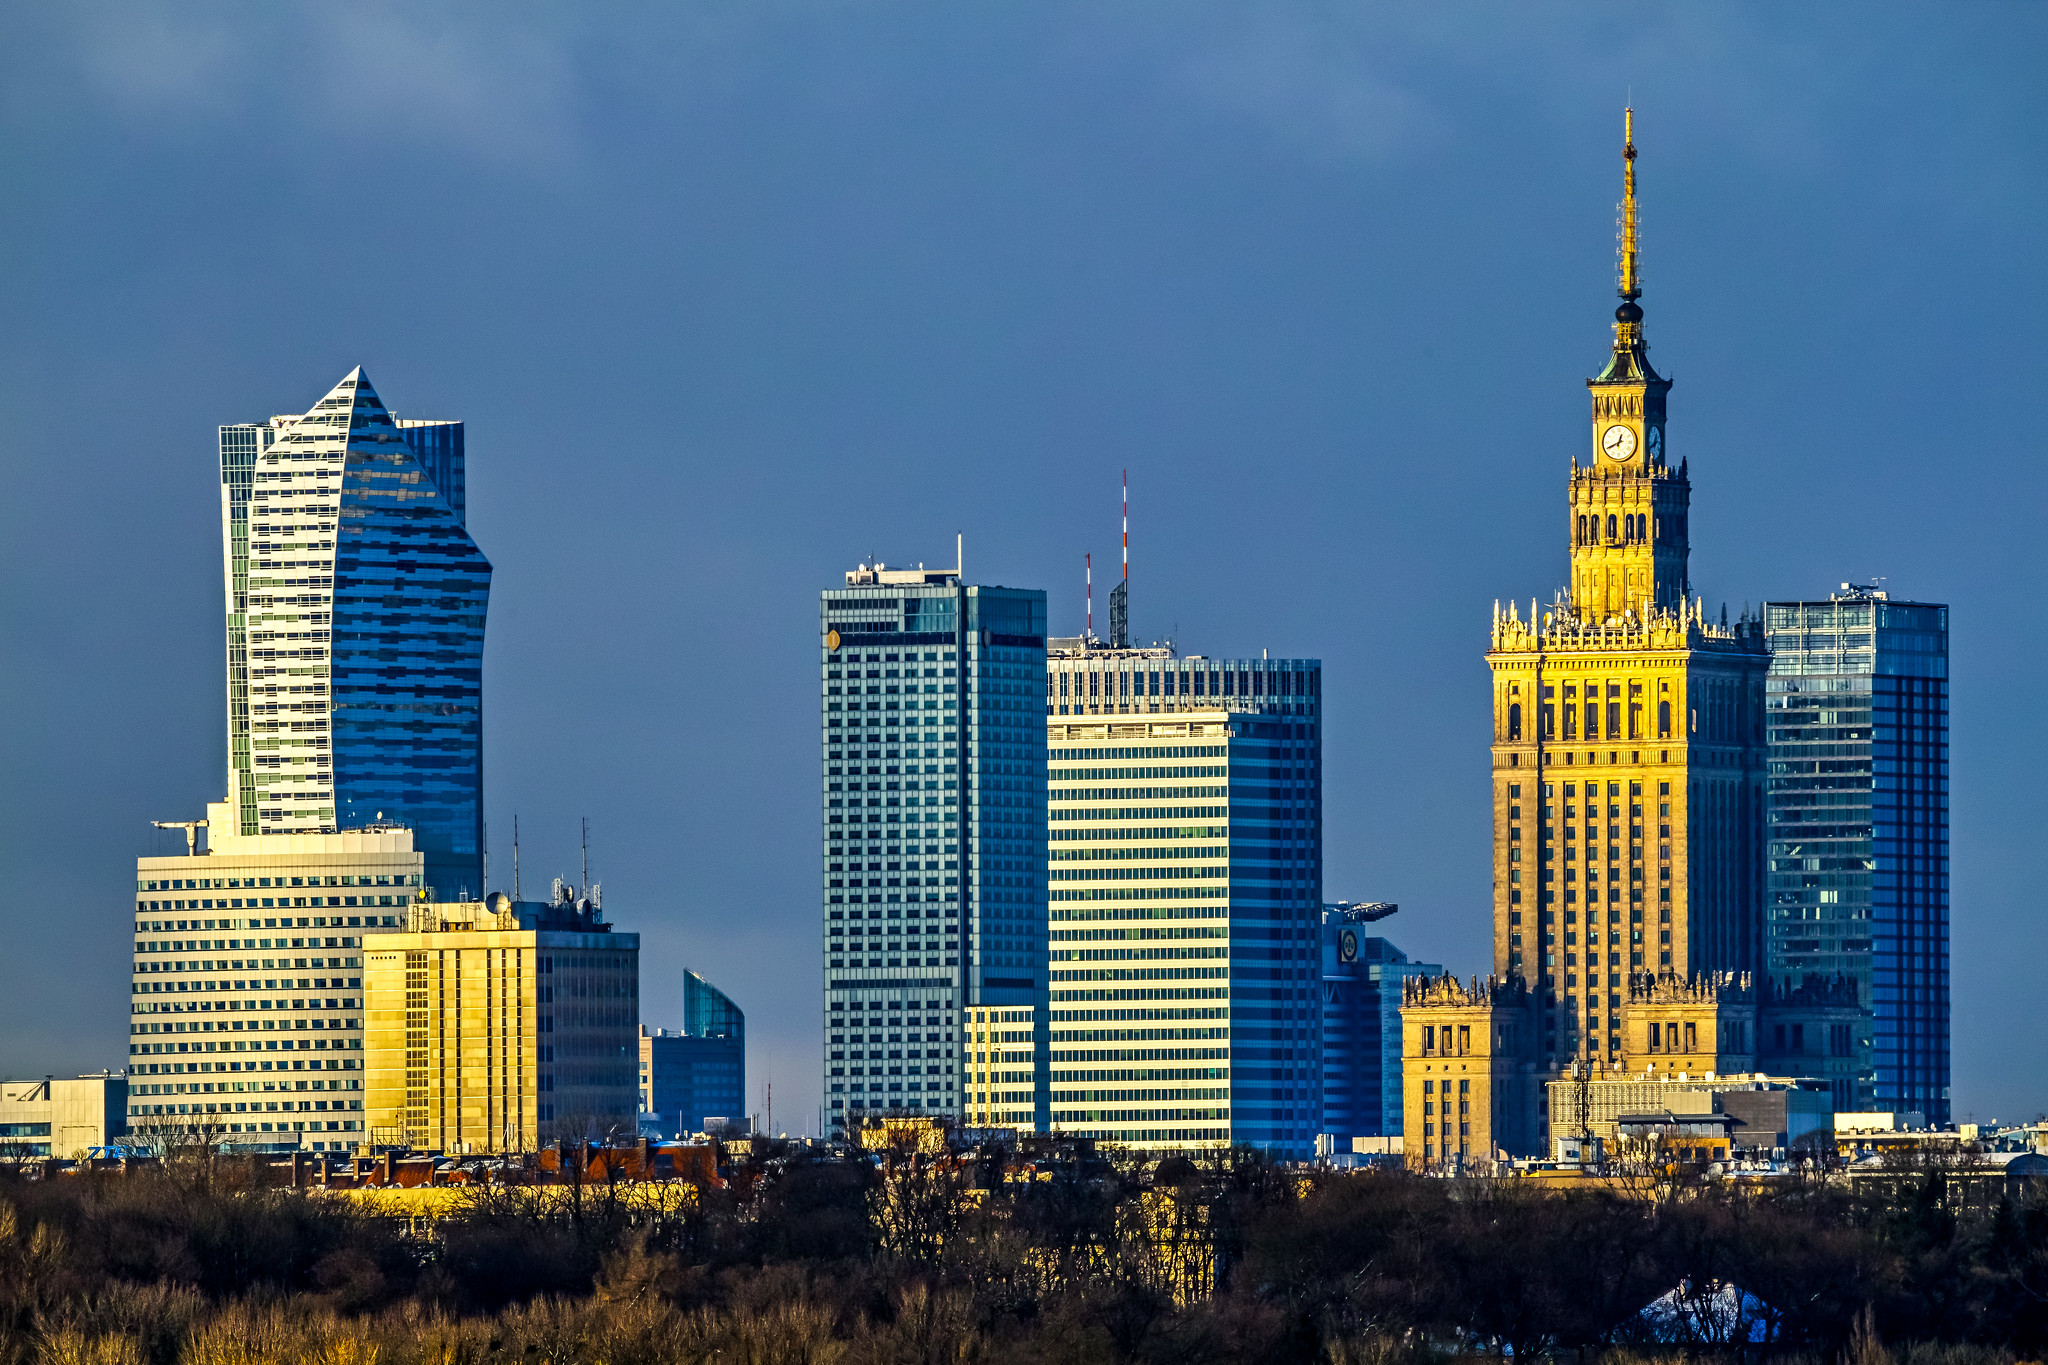
\includegraphics{figure/am1974_flicker.jpg}
\caption{Warsaw skyscrapers by Artur Malinowski Flicker}
\end{figure}

Predicting house prices is a common exercise used in machine-learning
courses. Various datasets for house prices are available at websites
like Kaggle (\url{https://www.kaggle.com}) or UCI Machine Learning
Repository (\url{https://archive.ics.uci.edu}).

In this book we will work with an interesting version of this problem.
The \texttt{apartments} dataset is an artificial dataset created to
match key characteristics of real apartments in Warszawa, the capital of
Poland. However, the dataset is created in a way that two very different
models, namely linear regression and random forest, have almost exactly
the same accuracy. The natural question is which model should we choose?
We will show that the model-explanation tools provide important insight
into the key model characteristics and are helpful in model selection.

The dataset is available in the \texttt{DALEX} package \citep{R-DALEX}.
It contains 1000 observations (apartments) and six variables:

\begin{itemize}
\tightlist
\item
  \emph{m2.price}, apatments price per meter-squared (in EUR), a
  numerical variable
\item
  \emph{construction.year}, the year of construction of the block of
  flats in which the apartment is located, a numerical variable
\item
  \emph{surface}, apartment's total surface in squared meters, a
  numerical variable
\item
  \emph{floor}, the floor at which the apartment is located (ground
  floor taken to be the first floor), a numerical integer variable with
  values from 1 to 10
\item
  \emph{no.rooms}, the total number of rooms, a numerical variable with
  values from 1 to 6
\item
  \emph{distric}, a factor with 10 levels indicating tha distric of
  Warszawa where the apartment is located
\end{itemize}

Models considered for this dataset will use \emph{m2.price} as the
(continuous) dependent variable.

\begin{Shaded}
\begin{Highlighting}[]
\KeywordTok{library}\NormalTok{(}\StringTok{"DALEX"}\NormalTok{)}
\KeywordTok{head}\NormalTok{(apartments, }\DecValTok{2}\NormalTok{)}
\end{Highlighting}
\end{Shaded}

\begin{verbatim}
##   m2.price construction.year surface floor no.rooms    district
## 1     5897              1953      25     3        1 Srodmiescie
## 2     1818              1992     143     9        5     Bielany
\end{verbatim}

\begin{Shaded}
\begin{Highlighting}[]
\KeywordTok{str}\NormalTok{(apartments)}
\end{Highlighting}
\end{Shaded}

\begin{verbatim}
## 'data.frame':    1000 obs. of  6 variables:
##  $ m2.price         : num  5897 1818 3643 3517 3013 ...
##  $ construction.year: num  1953 1992 1937 1995 1992 ...
##  $ surface          : num  25 143 56 93 144 61 127 105 145 112 ...
##  $ floor            : int  3 9 1 7 6 6 8 8 6 9 ...
##  $ no.rooms         : num  1 5 2 3 5 2 5 4 6 4 ...
##  $ district         : Factor w/ 10 levels "Bemowo","Bielany",..: 6 2 5 4 3 6 3 7 6 6 ...
\end{verbatim}

\begin{Shaded}
\begin{Highlighting}[]
\KeywordTok{table}\NormalTok{(apartments}\OperatorTok{$}\NormalTok{floor)}
\end{Highlighting}
\end{Shaded}

\begin{verbatim}
## 
##   1   2   3   4   5   6   7   8   9  10 
##  90 116  87  86  95 104 103 103 108 108
\end{verbatim}

\begin{Shaded}
\begin{Highlighting}[]
\KeywordTok{table}\NormalTok{(apartments}\OperatorTok{$}\NormalTok{no.rooms)}
\end{Highlighting}
\end{Shaded}

\begin{verbatim}
## 
##   1   2   3   4   5   6 
##  99 202 231 223 198  47
\end{verbatim}

\begin{Shaded}
\begin{Highlighting}[]
\KeywordTok{levels}\NormalTok{(apartments}\OperatorTok{$}\NormalTok{district)}
\end{Highlighting}
\end{Shaded}

\begin{verbatim}
##  [1] "Bemowo"      "Bielany"     "Mokotow"     "Ochota"      "Praga"      
##  [6] "Srodmiescie" "Ursus"       "Ursynow"     "Wola"        "Zoliborz"
\end{verbatim}

Model predictions will be obtained for a set of six apartments included
in data frame \texttt{apartments\_test}, also included in the
\texttt{DALEX} package.

\begin{Shaded}
\begin{Highlighting}[]
\KeywordTok{head}\NormalTok{(apartments_test)}
\end{Highlighting}
\end{Shaded}

\begin{verbatim}
##      m2.price construction.year surface floor no.rooms    district
## 1001     4644              1976     131     3        5 Srodmiescie
## 1002     3082              1978     112     9        4     Mokotow
## 1003     2498              1958     100     7        4     Bielany
## 1004     2735              1951     112     3        5        Wola
## 1005     2781              1978     102     4        4      Bemowo
## 1006     2936              2001     116     7        4      Bemowo
\end{verbatim}

\hypertarget{data-exploration-1}{%
\subsubsection{Data exploration}\label{data-exploration-1}}

{[}TOMASZ: TO ADD, EVEN IF SHORT{]}

\hypertarget{model_apartments_lr}{%
\subsubsection{Linear regression}\label{model_apartments_lr}}

The dependent variable of interest, \emph{m2.price}, is continuous.
Thus, a natural choice to build a predictive model is linear regression.
We treat all the other variables in the \texttt{apartments} data frame
as explanatory and include them in the model. The results of the model
are stored in model-object \texttt{apartments\_lm\_v5}.

\begin{Shaded}
\begin{Highlighting}[]
\NormalTok{apartments_lm_v5 <-}\StringTok{ }\KeywordTok{lm}\NormalTok{(m2.price }\OperatorTok{~}\StringTok{ }\NormalTok{., }\DataTypeTok{data =}\NormalTok{ apartments)}
\NormalTok{apartments_lm_v5}
\end{Highlighting}
\end{Shaded}

\begin{verbatim}
## 
## Call:
## lm(formula = m2.price ~ ., data = apartments)
## 
## Coefficients:
##         (Intercept)    construction.year              surface  
##            5020.139               -0.229              -10.238  
##               floor             no.rooms      districtBielany  
##             -99.482              -37.730               17.214  
##     districtMokotow       districtOchota        districtPraga  
##             918.380              926.254              -37.105  
## districtSrodmiescie        districtUrsus      districtUrsynow  
##            2080.611               29.942              -18.865  
##        districtWola     districtZoliborz  
##             -16.891              889.973
\end{verbatim}

\hypertarget{model_apartments_rf}{%
\subsubsection{Random forest}\label{model_apartments_rf}}

As an alternative to linear regression, we consider a random forest
model. To fit the model, we apply the \texttt{randomForest()} function,
with default settings, from the package with the same name
\citep{randomForestRNews}.\\
The results of the model are stored in model-object
\texttt{apartments\_rf\_v5}.

\begin{Shaded}
\begin{Highlighting}[]
\KeywordTok{library}\NormalTok{(}\StringTok{"randomForest"}\NormalTok{)}
\KeywordTok{set.seed}\NormalTok{(}\DecValTok{72}\NormalTok{)}
\NormalTok{apartments_rf_v5 <-}\StringTok{ }\KeywordTok{randomForest}\NormalTok{(m2.price }\OperatorTok{~}\StringTok{ }\NormalTok{., }\DataTypeTok{data =}\NormalTok{ apartments)}
\NormalTok{apartments_rf_v5}
\end{Highlighting}
\end{Shaded}

\begin{verbatim}
## 
## Call:
##  randomForest(formula = m2.price ~ ., data = apartments) 
##                Type of random forest: regression
##                      Number of trees: 500
## No. of variables tried at each split: 1
## 
##           Mean of squared residuals: 79789.39
##                     % Var explained: 90.28
\end{verbatim}

\hypertarget{predictions_apartments}{%
\subsubsection{Model predictions}\label{predictions_apartments}}

By aplying the \texttt{predict()} function to model-object
\texttt{apartments\_lm\_v5} with \texttt{apartments\_test} as the data
frame for which predictions are to be computed, we obtain the predicted
prices for the testing set of six apartments for the linear regression
model. Subsequently, we compute the mean squared difference between the
predicted and actual prices for the test apartments. We repeat the same
steps for the random forest model.

\begin{Shaded}
\begin{Highlighting}[]
\NormalTok{predicted_apartments_lm <-}\StringTok{ }\KeywordTok{predict}\NormalTok{(apartments_lm_v5, apartments_test)}
\NormalTok{rmsd_lm <-}\StringTok{ }\KeywordTok{sqrt}\NormalTok{(}\KeywordTok{mean}\NormalTok{((predicted_apartments_lm }\OperatorTok{-}\StringTok{ }\NormalTok{apartments_test}\OperatorTok{$}\NormalTok{m2.price)}\OperatorTok{^}\DecValTok{2}\NormalTok{))}
\NormalTok{rmsd_lm}
\end{Highlighting}
\end{Shaded}

\begin{verbatim}
## [1] 283.0865
\end{verbatim}

\begin{Shaded}
\begin{Highlighting}[]
\KeywordTok{library}\NormalTok{(}\StringTok{"randomForest"}\NormalTok{)}
\NormalTok{predicted_apartments_rf <-}\StringTok{ }\KeywordTok{predict}\NormalTok{(apartments_rf_v5, apartments_test)}
\NormalTok{rmsd_rf <-}\StringTok{ }\KeywordTok{sqrt}\NormalTok{(}\KeywordTok{mean}\NormalTok{((predicted_apartments_rf }\OperatorTok{-}\StringTok{ }\NormalTok{apartments_test}\OperatorTok{$}\NormalTok{m2.price)}\OperatorTok{^}\DecValTok{2}\NormalTok{))}
\NormalTok{rmsd_rf}
\end{Highlighting}
\end{Shaded}

\begin{verbatim}
## [1] 282.9519
\end{verbatim}

For the random forest model, the square-root of the mean squared
difference is equal to 283. It is only minimally smaller than the value
of 283.1, obtained for the linear regression model. Thus, the question
we may face is: should we choose the model complex, but flexible
random-forest model, or the simpler and easier to interpret linear
model? In the subsequent chapters we will try to provide an answer to
this question.

\hypertarget{HFDataset}{%
\subsection{Hire or fire}\label{HFDataset}}

Predictive models can be used to support decisions. For instance, they
could be used in a human-resources department to decide whether, for
instance, promote an employee. An advantage of using a model for this
purpose would be the objectivity of the decision, which would not be
subject to personal preferences of a manager. However, in such a
situation, one would most likely want to understand what influences the
model's prediction.

To illustrate such a situation, we will use the \texttt{HR} dataset that
is available in the \texttt{DALEX} package \citep{R-DALEX}. It is an
artificial set of data from a human-resources department of a call
center. It contains 7847 observations (employees of the call center) and
six variables:

\begin{itemize}
\tightlist
\item
  \emph{gender}, person's gender, a factor with two levels
\item
  \emph{age}, person's age in years, a numerical variable
\item
  \emph{hours}, average number of working hours per week, a numerical
  variable
\item
  \emph{evaluation}, the last evaluation score, a numerical variable
  with values 2 (fail), 3 (satisfactory), 4 (good), and 5 (veru good)
  {[}TOMASZ: CORRECT?{]}
\item
  \emph{salary}, the salary level, a numerical variable with values from
  0 to 5 {[}TOMASZ: WHAT DOES 0 MEAN?{]}
\item
  \emph{status}, a factor with three indicating whether the employee was
  fired, retained, or promoted
\end{itemize}

Models considered for this dataset will use \emph{status} as the
(categorical) dependent variable.

\begin{Shaded}
\begin{Highlighting}[]
\KeywordTok{library}\NormalTok{(}\StringTok{"DALEX"}\NormalTok{)}
\KeywordTok{head}\NormalTok{(HR, }\DecValTok{4}\NormalTok{)}
\end{Highlighting}
\end{Shaded}

\begin{verbatim}
##   gender      age    hours evaluation salary status
## 1   male 32.58267 41.88626          3      1  fired
## 2 female 41.21104 36.34339          2      5  fired
## 3   male 37.70516 36.81718          3      0  fired
## 4 female 30.06051 38.96032          3      2  fired
\end{verbatim}

\begin{Shaded}
\begin{Highlighting}[]
\KeywordTok{str}\NormalTok{(HR)}
\end{Highlighting}
\end{Shaded}

\begin{verbatim}
## 'data.frame':    7847 obs. of  6 variables:
##  $ gender    : Factor w/ 2 levels "female","male": 2 1 2 1 2 2 1 2 1 1 ...
##  $ age       : num  32.6 41.2 37.7 30.1 21.1 ...
##  $ hours     : num  41.9 36.3 36.8 39 62.2 ...
##  $ evaluation: num  3 2 3 3 5 2 4 2 2 4 ...
##  $ salary    : num  1 5 0 2 3 0 0 4 4 4 ...
##  $ status    : Factor w/ 3 levels "fired","ok","promoted": 1 1 1 1 3 1 3 2 1 3 ...
\end{verbatim}

\begin{Shaded}
\begin{Highlighting}[]
\KeywordTok{table}\NormalTok{(HR}\OperatorTok{$}\NormalTok{evaluation)}
\end{Highlighting}
\end{Shaded}

\begin{verbatim}
## 
##    2    3    4    5 
## 2371 2272 1661 1543
\end{verbatim}

\begin{Shaded}
\begin{Highlighting}[]
\KeywordTok{table}\NormalTok{(HR}\OperatorTok{$}\NormalTok{salary)}
\end{Highlighting}
\end{Shaded}

\begin{verbatim}
## 
##    0    1    2    3    4    5 
## 1105 1417 1461 1508 1316 1040
\end{verbatim}

\hypertarget{model_HR_mr}{%
\subsubsection{Multinomial logistic regression}\label{model_HR_mr}}

The dependent variable of interest, \emph{status}, is categorical with
three categories. Thus, a simple choice is to consider a multinomial
logistic regression model {[}TOMASZ: REFERENCE{]}. We fit the model with
the help of function \texttt{multinom} from package \texttt{nnet}. The
function fits multinomial log-linear models by using the neural-networks
approach. {[}TOMASZ: WHY THIS APPROACH?{]} We treat all variables other
than \texttt{status} in the \texttt{HR} data frame as explanatory and
include them in the model. The results of the model are stored in
model-object \texttt{HR\_glm\_v5}.

\begin{Shaded}
\begin{Highlighting}[]
\KeywordTok{library}\NormalTok{(}\StringTok{"nnet"}\NormalTok{)}
\NormalTok{HR_glm_v5 <-}\StringTok{ }\KeywordTok{multinom}\NormalTok{(status }\OperatorTok{~}\StringTok{ }\NormalTok{gender }\OperatorTok{+}\StringTok{ }\NormalTok{age }\OperatorTok{+}\StringTok{ }\NormalTok{hours }\OperatorTok{+}\StringTok{ }\NormalTok{evaluation }\OperatorTok{+}\StringTok{ }\NormalTok{salary, }\DataTypeTok{data =}\NormalTok{ HR)}
\end{Highlighting}
\end{Shaded}

\begin{verbatim}
## # weights:  21 (12 variable)
## initial  value 8620.810629 
## iter  10 value 7002.127738
## iter  20 value 6239.478146
## iter  20 value 6239.478126
## iter  20 value 6239.478124
## final  value 6239.478124 
## converged
\end{verbatim}

\begin{Shaded}
\begin{Highlighting}[]
\NormalTok{HR_glm_v5}
\end{Highlighting}
\end{Shaded}

\begin{verbatim}
## Call:
## multinom(formula = status ~ gender + age + hours + evaluation + 
##     salary, data = HR)
## 
## Coefficients:
##          (Intercept) gendermale         age      hours  evaluation
## ok         -3.199741 0.05185293 0.001003521 0.06628055 -0.03734345
## promoted  -12.677639 0.11838037 0.003436872 0.16253343  1.26109093
##              salary
## ok       0.01680039
## promoted 0.01507927
## 
## Residual Deviance: 12478.96 
## AIC: 12502.96
\end{verbatim}

\hypertarget{model_HR_rf}{%
\subsubsection{Random forest}\label{model_HR_rf}}

As an alternative to multinomial logisitc regression, we consider a
random forest model. To fit the model, we apply the
\texttt{randomForest()} function, with default settings, from the
package with the same name \citep{randomForestRNews}. The results of the
model are stored in model-object \texttt{HR\_rf\_v5}.

\begin{Shaded}
\begin{Highlighting}[]
\KeywordTok{set.seed}\NormalTok{(}\DecValTok{59}\NormalTok{)}
\KeywordTok{library}\NormalTok{(}\StringTok{"randomForest"}\NormalTok{)}
\NormalTok{HR_rf_v5 <-}\StringTok{ }\KeywordTok{randomForest}\NormalTok{(status }\OperatorTok{~}\StringTok{ }\NormalTok{gender }\OperatorTok{+}\StringTok{ }\NormalTok{age }\OperatorTok{+}\StringTok{ }\NormalTok{hours }\OperatorTok{+}\StringTok{ }\NormalTok{evaluation }\OperatorTok{+}\StringTok{ }\NormalTok{salary, }\DataTypeTok{data =}\NormalTok{ HR)}
\NormalTok{HR_rf_v5}
\end{Highlighting}
\end{Shaded}

\begin{verbatim}
## 
## Call:
##  randomForest(formula = status ~ gender + age + hours + evaluation +      salary, data = HR) 
##                Type of random forest: classification
##                      Number of trees: 500
## No. of variables tried at each split: 2
## 
##         OOB estimate of  error rate: 27.31%
## Confusion matrix:
##          fired   ok promoted class.error
## fired     2274  384      197   0.2035026
## ok         525 1255      441   0.4349392
## promoted   201  395     2175   0.2150848
\end{verbatim}

\hypertarget{predictions_HR}{%
\subsubsection{Model predictions}\label{predictions_HR}}

{[}TOMASZ: TO ADD{]}

\hypertarget{ListOfModels}{%
\subsection{List of models}\label{ListOfModels}}

In the previous sections we have built several predictive models for
differnt datasets. The models will be used in the rest of the book to
illustrate the mdoel explanation methods and tools. For the ease of
reference, we summarize the models in the table beloW. The binary
model-objects can be donwloaded by using the attached \texttt{archivist}
hooks \citep{archivist}. {[}TOMASZ: THIS IS USEFUL FOR E-BOOK. HOW ABOUT
THE PRINTED VERSION?{]}

\begin{longtable}[]{@{}lllll@{}}
\toprule
\begin{minipage}[b]{0.20\columnwidth}\raggedright
Model name\strut
\end{minipage} & \begin{minipage}[b]{0.24\columnwidth}\raggedright
Model generator\strut
\end{minipage} & \begin{minipage}[b]{0.14\columnwidth}\raggedright
Dataset\strut
\end{minipage} & \begin{minipage}[b]{0.17\columnwidth}\raggedright
Variables\strut
\end{minipage} & \begin{minipage}[b]{0.10\columnwidth}\raggedright
Link to the model\strut
\end{minipage}\tabularnewline
\midrule
\endhead
\begin{minipage}[t]{0.20\columnwidth}\raggedright
\texttt{titanic\_lmr\_v6}\strut
\end{minipage} & \begin{minipage}[t]{0.24\columnwidth}\raggedright
\texttt{rms::\ lmr}\strut
\end{minipage} & \begin{minipage}[t]{0.14\columnwidth}\raggedright
\texttt{DALEX::\ titanic}\strut
\end{minipage} & \begin{minipage}[t]{0.17\columnwidth}\raggedright
gender, age, class, sibsp, parch, fare, embarked\strut
\end{minipage} & \begin{minipage}[t]{0.10\columnwidth}\raggedright
\texttt{archivist::\ aread("pbiecek/models/f285c")}\strut
\end{minipage}\tabularnewline
\begin{minipage}[t]{0.20\columnwidth}\raggedright
\texttt{titanic\_rf\_v6}\strut
\end{minipage} & \begin{minipage}[t]{0.24\columnwidth}\raggedright
\texttt{randomForest::\ randomForest}\strut
\end{minipage} & \begin{minipage}[t]{0.14\columnwidth}\raggedright
\texttt{DALEX::\ titanic}\strut
\end{minipage} & \begin{minipage}[t]{0.17\columnwidth}\raggedright
gender, age, class, sibsp, parch, fare, embarked\strut
\end{minipage} & \begin{minipage}[t]{0.10\columnwidth}\raggedright
\texttt{archivist::\ aread("pbiecek/models/92753")}\strut
\end{minipage}\tabularnewline
\begin{minipage}[t]{0.20\columnwidth}\raggedright
\texttt{titanic\_rf\_v3}\strut
\end{minipage} & \begin{minipage}[t]{0.24\columnwidth}\raggedright
\texttt{randomForest::\ randomForest}\strut
\end{minipage} & \begin{minipage}[t]{0.14\columnwidth}\raggedright
\texttt{DALEX::\ titanic}\strut
\end{minipage} & \begin{minipage}[t]{0.17\columnwidth}\raggedright
gender, age, class\strut
\end{minipage} & \begin{minipage}[t]{0.10\columnwidth}\raggedright
\texttt{archivist::\ aread("pbiecek/models/bcd20")}\strut
\end{minipage}\tabularnewline
\begin{minipage}[t]{0.20\columnwidth}\raggedright
\texttt{titanic\_gbm\_v6}\strut
\end{minipage} & \begin{minipage}[t]{0.24\columnwidth}\raggedright
\texttt{gbm::\ gbm}\strut
\end{minipage} & \begin{minipage}[t]{0.14\columnwidth}\raggedright
\texttt{DALEX::\ titanic}\strut
\end{minipage} & \begin{minipage}[t]{0.17\columnwidth}\raggedright
gender, age, class, sibsp, parch, fare, embarked\strut
\end{minipage} & \begin{minipage}[t]{0.10\columnwidth}\raggedright
\texttt{archivist::\ aread("pbiecek/models/2bdad")}\strut
\end{minipage}\tabularnewline
\begin{minipage}[t]{0.20\columnwidth}\raggedright
\texttt{apartments\_lm\_v5}\strut
\end{minipage} & \begin{minipage}[t]{0.24\columnwidth}\raggedright
\texttt{stats::\ lm}\strut
\end{minipage} & \begin{minipage}[t]{0.14\columnwidth}\raggedright
\texttt{DALEX::\ apartments}\strut
\end{minipage} & \begin{minipage}[t]{0.17\columnwidth}\raggedright
construction .year, surface, floor, no.rooms, district\strut
\end{minipage} & \begin{minipage}[t]{0.10\columnwidth}\raggedright
\texttt{archivist::\ aread("pbiecek/models/55f19")}\strut
\end{minipage}\tabularnewline
\begin{minipage}[t]{0.20\columnwidth}\raggedright
\texttt{apartments\_rf\_v5}\strut
\end{minipage} & \begin{minipage}[t]{0.24\columnwidth}\raggedright
\texttt{randomForest::\ randomForest}\strut
\end{minipage} & \begin{minipage}[t]{0.14\columnwidth}\raggedright
\texttt{DALEX::\ apartments}\strut
\end{minipage} & \begin{minipage}[t]{0.17\columnwidth}\raggedright
construction .year, surface, floor, no.rooms, district\strut
\end{minipage} & \begin{minipage}[t]{0.10\columnwidth}\raggedright
\texttt{archivist::\ aread("pbiecek/models/fe7a5")}\strut
\end{minipage}\tabularnewline
\begin{minipage}[t]{0.20\columnwidth}\raggedright
\texttt{HR\_rf\_v5}\strut
\end{minipage} & \begin{minipage}[t]{0.24\columnwidth}\raggedright
\texttt{randomForest::\ randomForest}\strut
\end{minipage} & \begin{minipage}[t]{0.14\columnwidth}\raggedright
\texttt{DALEX::\ HR}\strut
\end{minipage} & \begin{minipage}[t]{0.17\columnwidth}\raggedright
gender, age, hours, evaluation, salary\strut
\end{minipage} & \begin{minipage}[t]{0.10\columnwidth}\raggedright
\texttt{archivist::\ aread("pbiecek/models/1ecfd")}\strut
\end{minipage}\tabularnewline
\begin{minipage}[t]{0.20\columnwidth}\raggedright
\texttt{HR\_glm\_v5}\strut
\end{minipage} & \begin{minipage}[t]{0.24\columnwidth}\raggedright
\texttt{stats::\ glm}\strut
\end{minipage} & \begin{minipage}[t]{0.14\columnwidth}\raggedright
\texttt{DALEX::\ HR}\strut
\end{minipage} & \begin{minipage}[t]{0.17\columnwidth}\raggedright
gender, age, hours, evaluation, salary\strut
\end{minipage} & \begin{minipage}[t]{0.10\columnwidth}\raggedright
\texttt{archivist::\ aread("pbiecek/models/f0244")}\strut
\end{minipage}\tabularnewline
\bottomrule
\end{longtable}

\hypertarget{instance-level-explanation}{%
\section*{Instance-level explanation}\label{instance-level-explanation}}
\addcontentsline{toc}{section}{Instance-level explanation}

\begin{figure}

{\centering 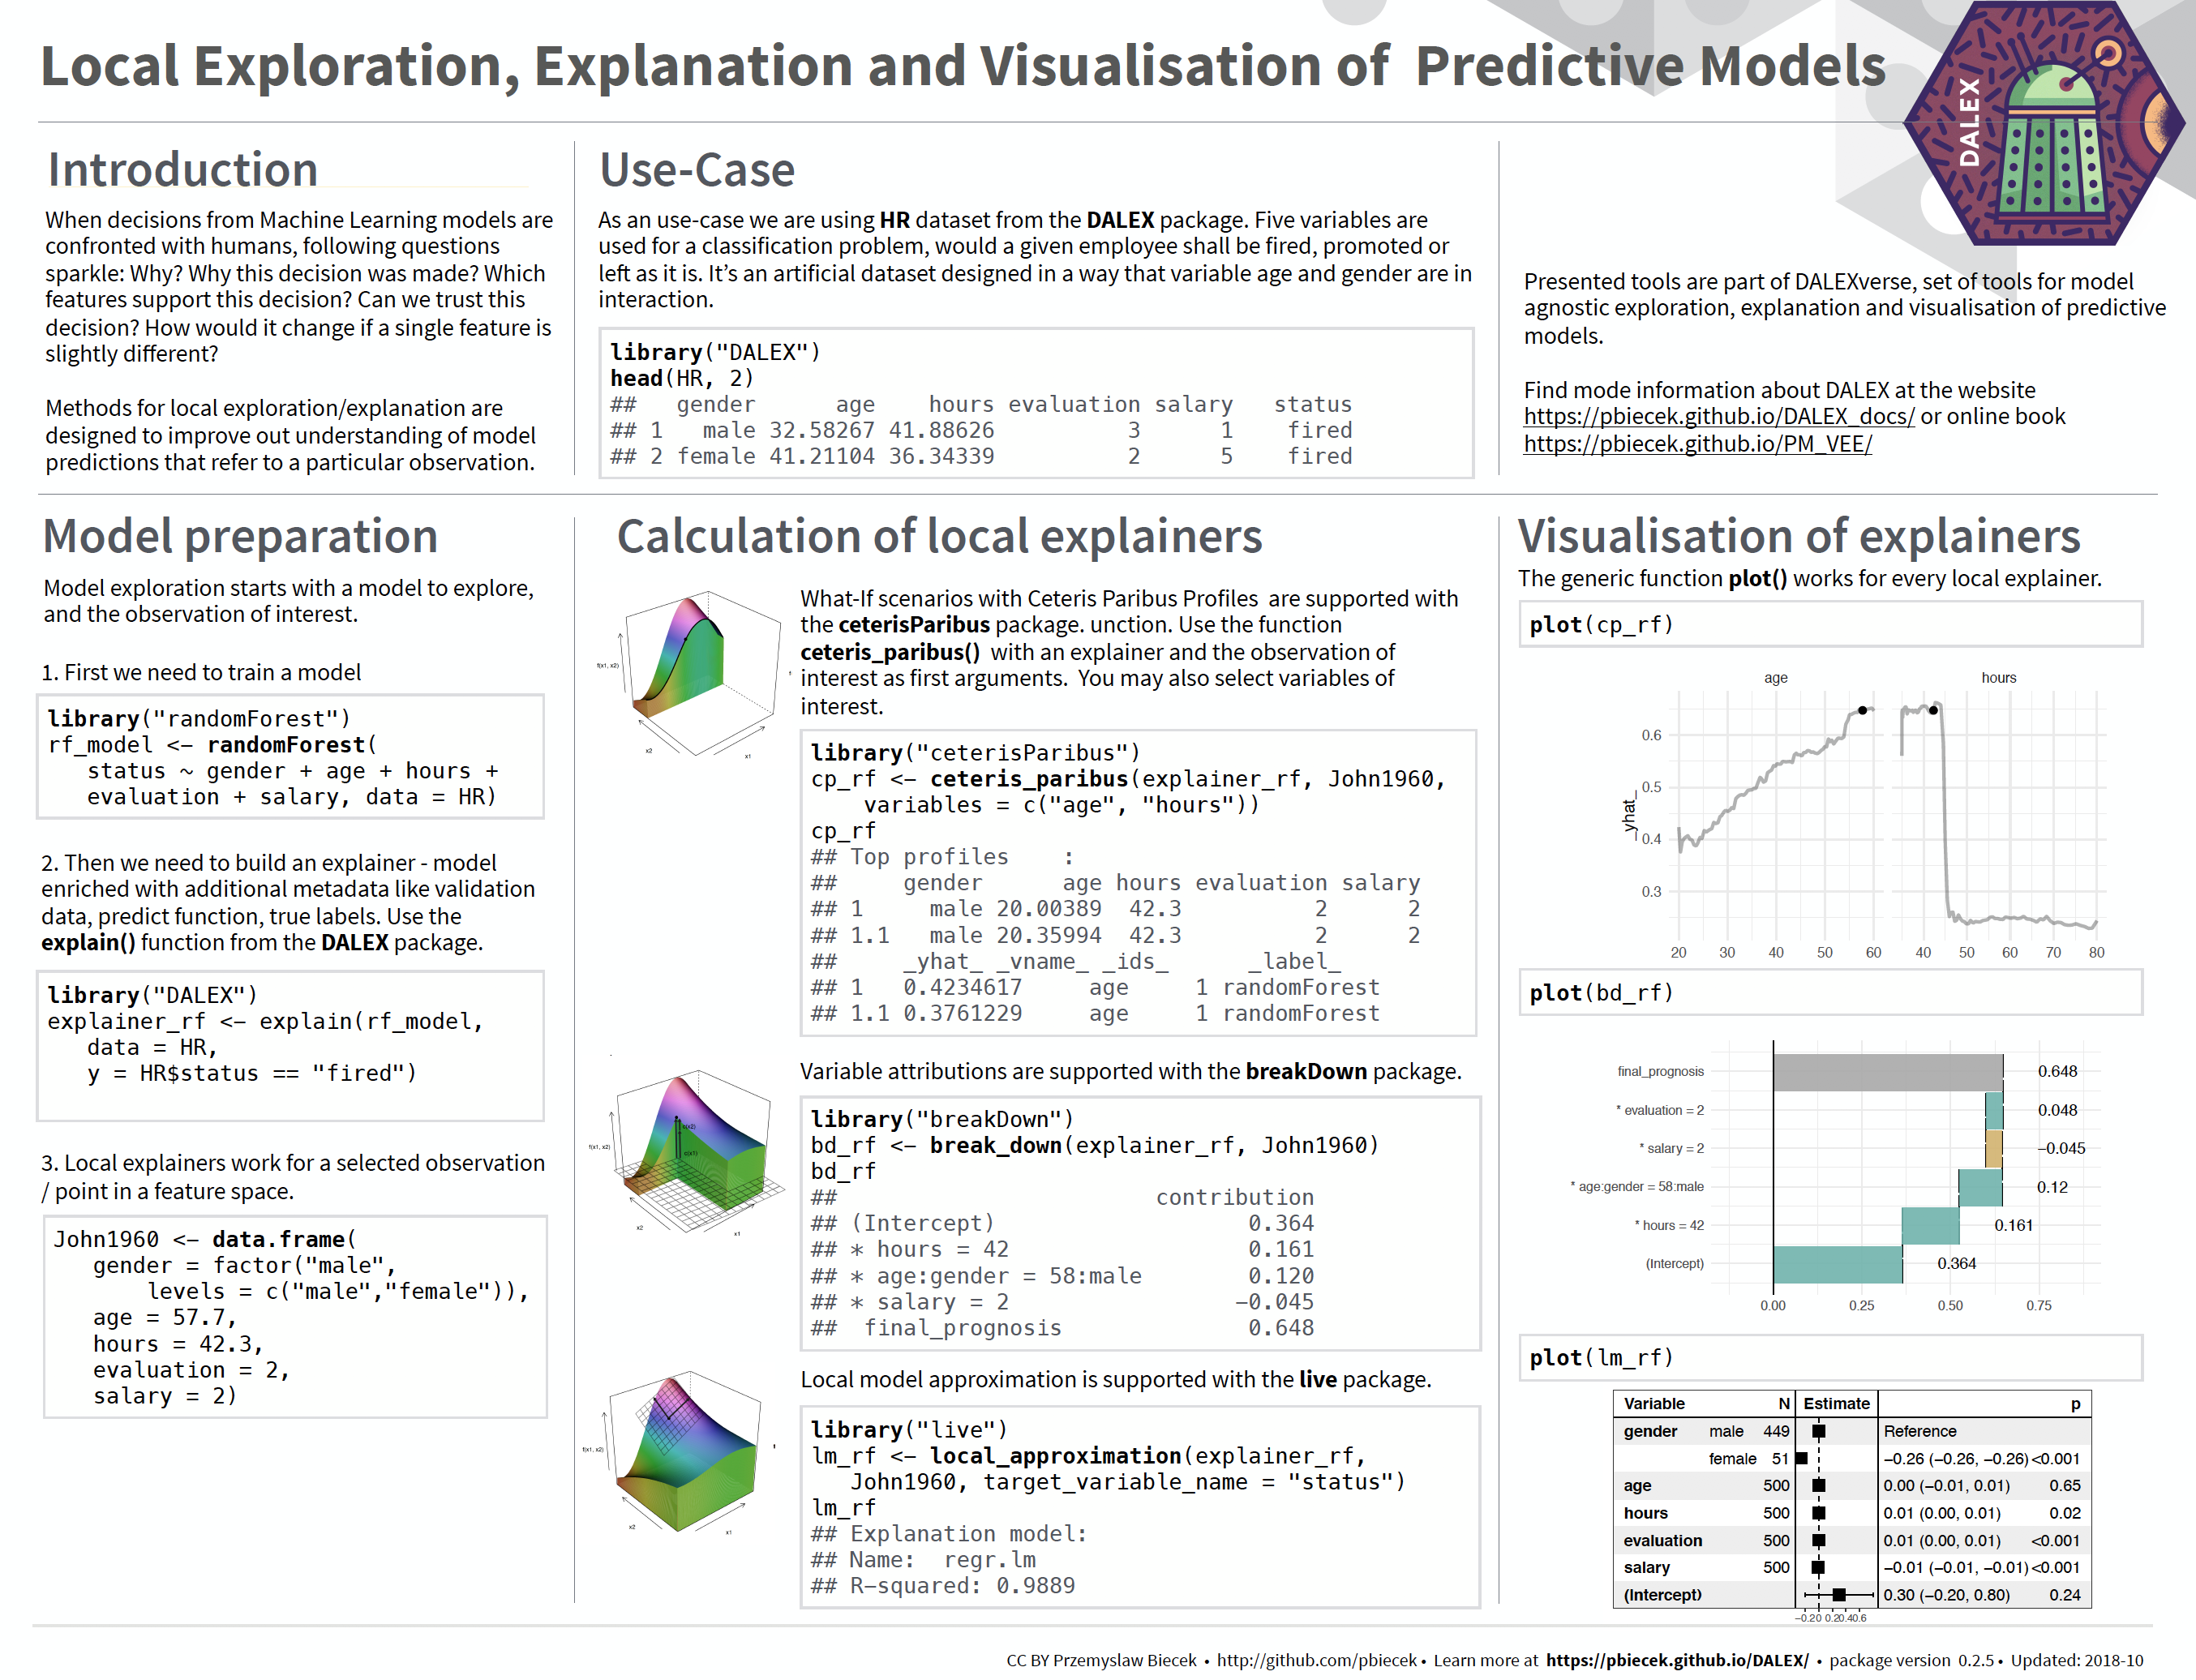
\includegraphics[width=0.99\linewidth]{figure/DALEX_local} 

}

\caption{(fig:localDALEXsummary) Summary of three approaches to local model exploration and explanation.}\label{fig:localDALEXsummary}
\end{figure}

\hypertarget{PredictionExplainers}{%
\section{Introduction}\label{PredictionExplainers}}

Instance-level explainers help to understand how a model yields a
prediction for a single observation. We can think about the following
situations as examples:

\begin{itemize}
\tightlist
\item
  We may want to evaluate the effects of explanatory variables on model
  predictions. For instance, we may be interested in predicting the risk
  of heart attack based on person's age, sex, and smoking habits. A
  model may be used to construct a score (for instance, a linear
  combination of the explanatory variables representing age, sex, and
  smoking habits) that could be used for the purposes of prediction. For
  a particular patient We may want to learn how much the different
  variables contribute to the patient's score?
\item
  We may want to understand how models predictions would change if
  values of some of the explanatory variables changed. For instance,
  what would be the predicted risk of heart attack if the patient cut
  the number of cigarettes smoked per day by half?
\item
  We may discover that the model is providing incorrect predictions and
  we may want to find the reason. For instance, a patient with a very
  low risk-score experiences heart attack. What has driven that
  prediction?
\end{itemize}

A model is a function with a \(p\)-dimensional vector \(x\) as an
argument. The plot of the value(s) of the function can be constructed in
a \(p+1\)-dimensional space. An example with \(p=2\) is presented in
Figure \ref{fig:cutsSurfaceReady}. We will use it as an illustration of
key ideas. The plot provides an information about the values of the
function in the vicinity of point \(x^*\).

\begin{figure}

{\centering 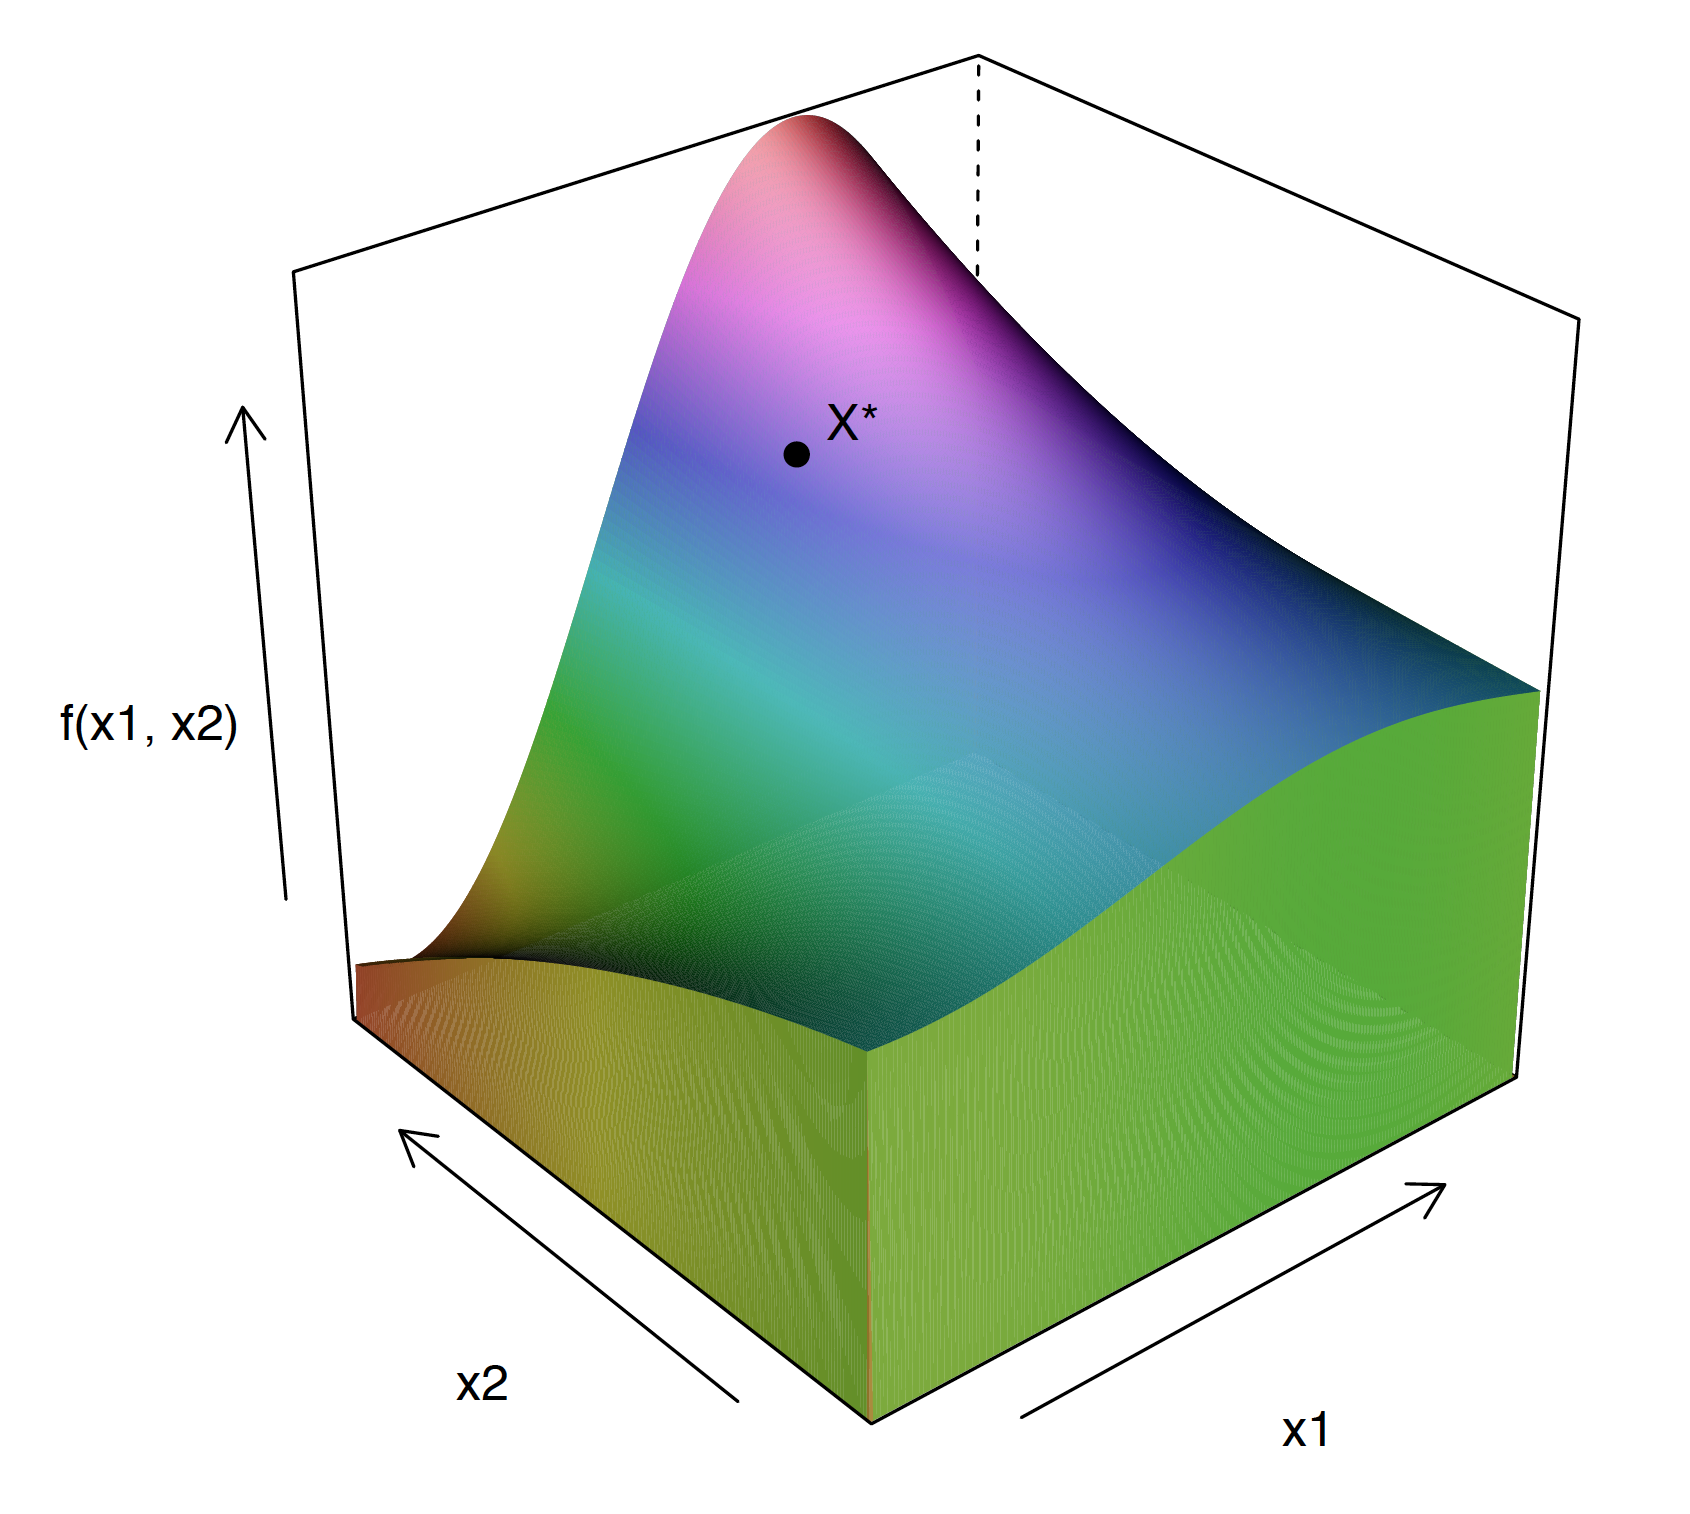
\includegraphics[width=0.6\linewidth]{figure/cuts_surface_ready_punkt} 

}

\caption{(fig:cutsSurfaceReady) Response surface for a model that is a function of two variables. We are interested in understanding the response of a model in a single point x*}\label{fig:cutsSurfaceReady}
\end{figure}

There are many different tools that may be used to explore the
predictions of the model around a single point \(x^*\). In the following
sections we will describe the most popular approaches. They can be
divided into three classes.

\begin{itemize}
\tightlist
\item
  One approach is to investigate how the model prediction changes if the
  value of a single explanatory variable changes. It is useful in the
  so-called ,,What-If'' scenarios. In particular, we can construct plots
  presenting the change of model-based predictions in function of a
  single variable. Such plots are usually called Ceteris Paribus
  profiles. They are presented in Chapter \ref{ceterisParibus}. An
  example is provided in panel A of Figure \ref{fig:cutsTechnikiReady}.
\item
  Another approach is to analyze the curvature of the response surface
  (see Figure \ref{fig:cutsSurfaceReady}) around the point of interest
  \(x^*\). Treating the model as a function, we are interested in the
  local behavior of this function around \(x^*\). In case of a black-box
  model, we approximate it with a simpler white-box model around
  \(x^*\). An example is provided in panel B of Figure
  \ref{fig:cutsTechnikiReady}. In Chapter \ref{LIME} we present the
  Local Interpretable Model-agnostic Explanations (LIME) method that
  exploits the concept of a ,,local model.''
\item
  Yet another approach is to analyze how the model prediction for point
  \(x^*\) is different from the average model prediction and how the
  difference can be distributed among the different dimensions
  (explanatory variables). It is often called the ,,variable
  attributions'' approach. An example is provided in panel C of Figure
  \ref{fig:cutsTechnikiReady}. In Chapter
  \ref{variableAttributionMethods} we present two methods implementing
  this approach, sequential conditioning and average conditioning (also
  called Shapley values).
\end{itemize}

\begin{figure}

{\centering 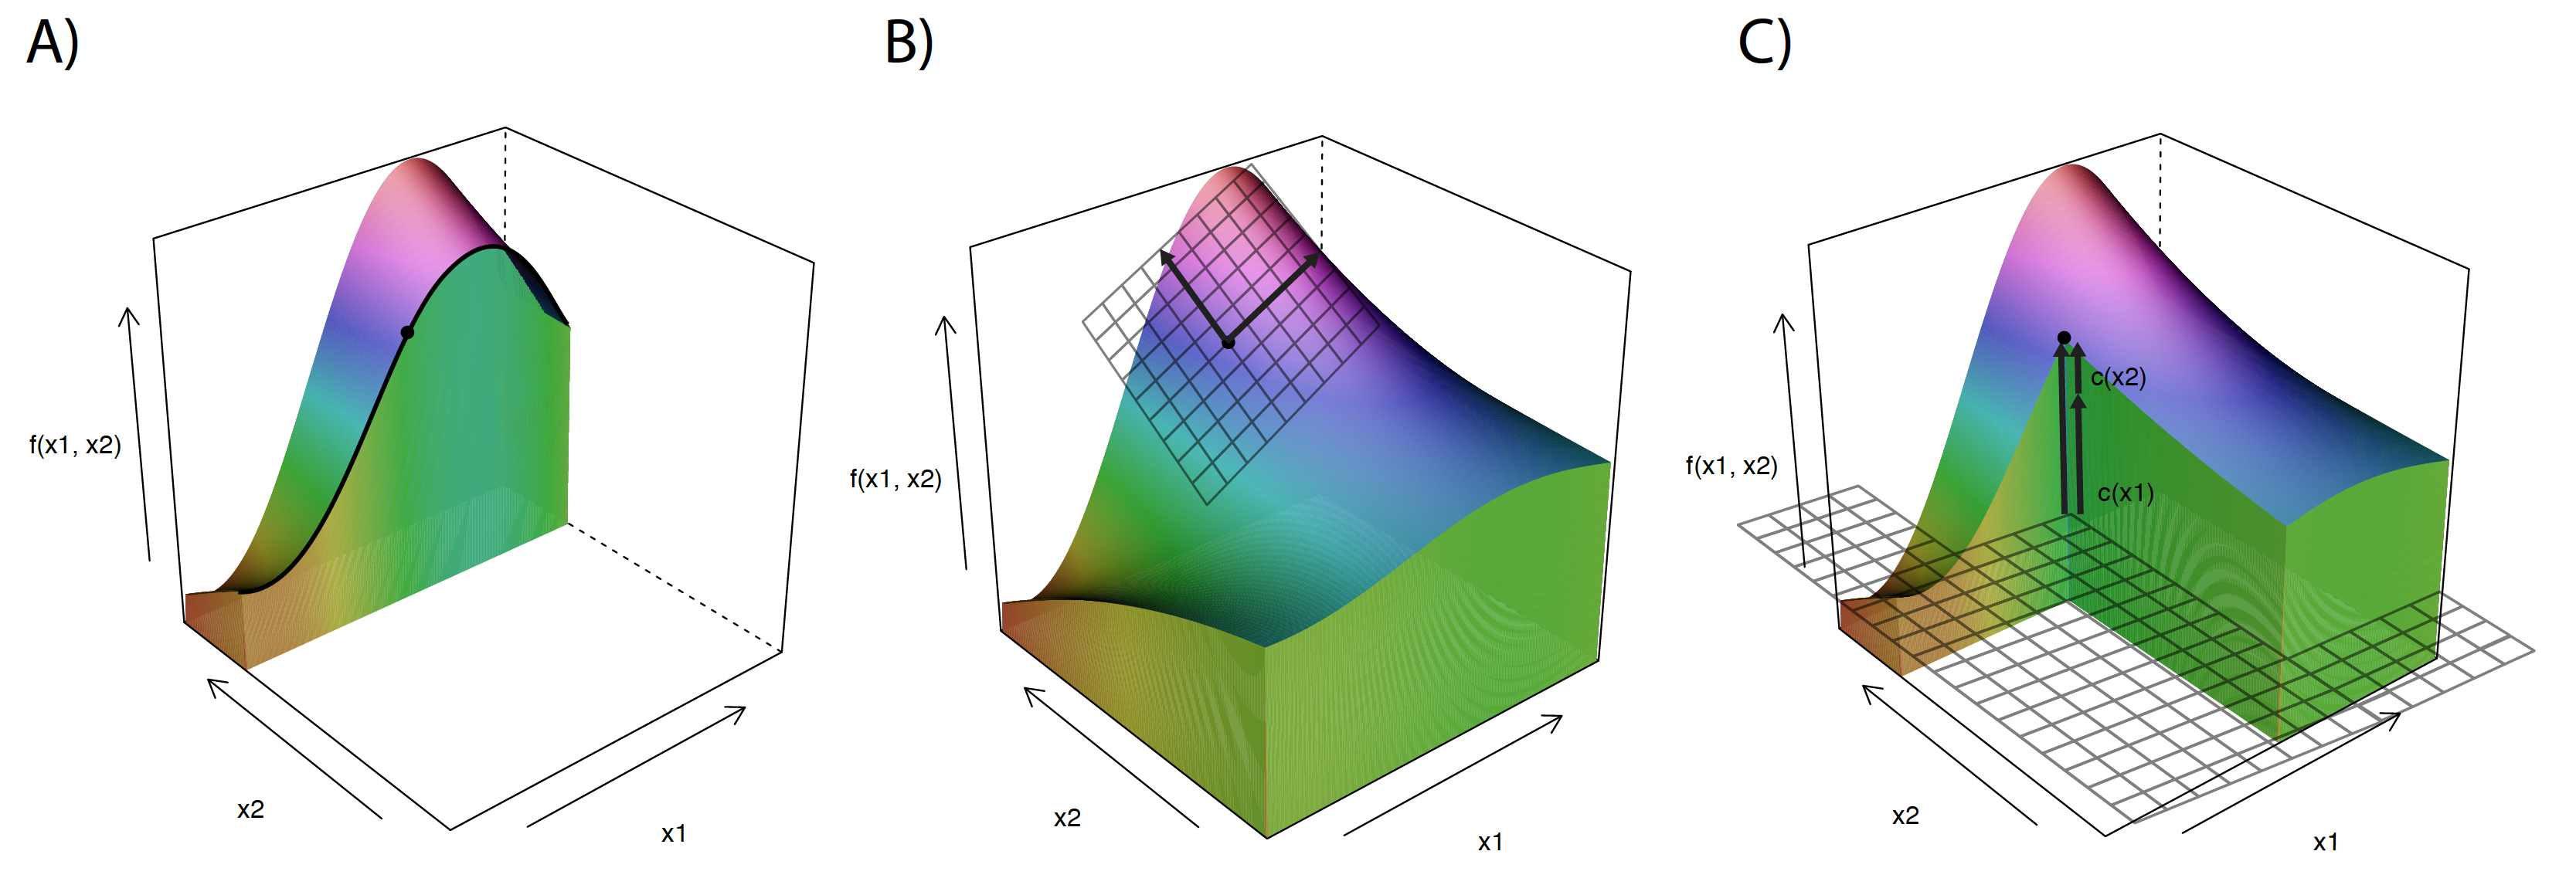
\includegraphics[width=0.99\linewidth]{figure/cuts_techniki_ready} 

}

\caption{(fig:cutsTechnikiReady) Illustration of different approaches to instance-level explanation. Panel A presents a What-If analysis with Ceteris Paribus profiles. The profiles plot the model response as a function of a value of a single variable, while keeping the values of all other explanatory variables fixed. Panel B illustrates the concept of local models. A simpler white-box model is fitted around the point of interest. It describes the local behaviour of the black-box model. Panel C illustrates the concept of variable attributions. Additive effects of each variable show how the model response differs from the average.}\label{fig:cutsTechnikiReady}
\end{figure}

\hypertarget{ceterisParibus}{%
\section{Ceteris Paribus Profiles - a tool for What-If
analysis}\label{ceterisParibus}}

\hypertarget{introduction-1}{%
\subsection{Introduction}\label{introduction-1}}

\emph{Ceteris paribus} is a Latin phrase meaning ``other things held
constant'' or ``all else unchanged.'' In this chapter, we introduce a
technique for model exploration based on the Ceteris paribus principle.
In particular, we examine the influence of each explanatory variable,
asumming that effects of all other variables are unchanged. The main
goal is to understand how changes in a single explanatory variable
affects model predictions.

Explainers presented in this chapter are linked to the second law
introduced in Section \ref{three-single-laws}, i.e.~the law of
``Prediction's speculation.'' This is why the tools are also known as
\emph{What-If model analysis} or \emph{Individual Conditional
Expectations} \citep{ICEbox}. It turns out that it is easier to
understand how a black-box model is working if we can explore the model
by investigating the influence of explanatory variables separately,
changing one at a time.

\hypertarget{intuition}{%
\subsection{Intuition}\label{intuition}}

Panel A of Figure \ref{fig:modelResponseCurveLine} presents response
(prediction) surface for the \texttt{titanic\_lmr\_v6} model for two
explanatory variables, \emph{age} and \emph{class}, from the
\emph{titanic} dataset (see Section \ref{TitanicDataset}). We are
interested in the change of the model prediction induced by each of the
variables. Toward this end, we may want to explore the curvature of the
response surface around a single point with \emph{age} equal to 47 and
\emph{class} equal to ``1st,'' indicated in the plot. Ceteris-paribus
(CP) profiles are one-dimensional profiles that examine the curvature
across each dimension, i.e., for each variable. Panel B of Figure
\ref{fig:modelResponseCurveLine} presents the profiles corresponding to
\emph{age} and \emph{class}. Note that, in the CP profile for
\emph{age}, the point of interest is indicated by the black dot. In
essence, a CP profile shows a conditional expectation of the dependent
variable (response) for the particular explanatory variable.

\begin{figure}

{\centering 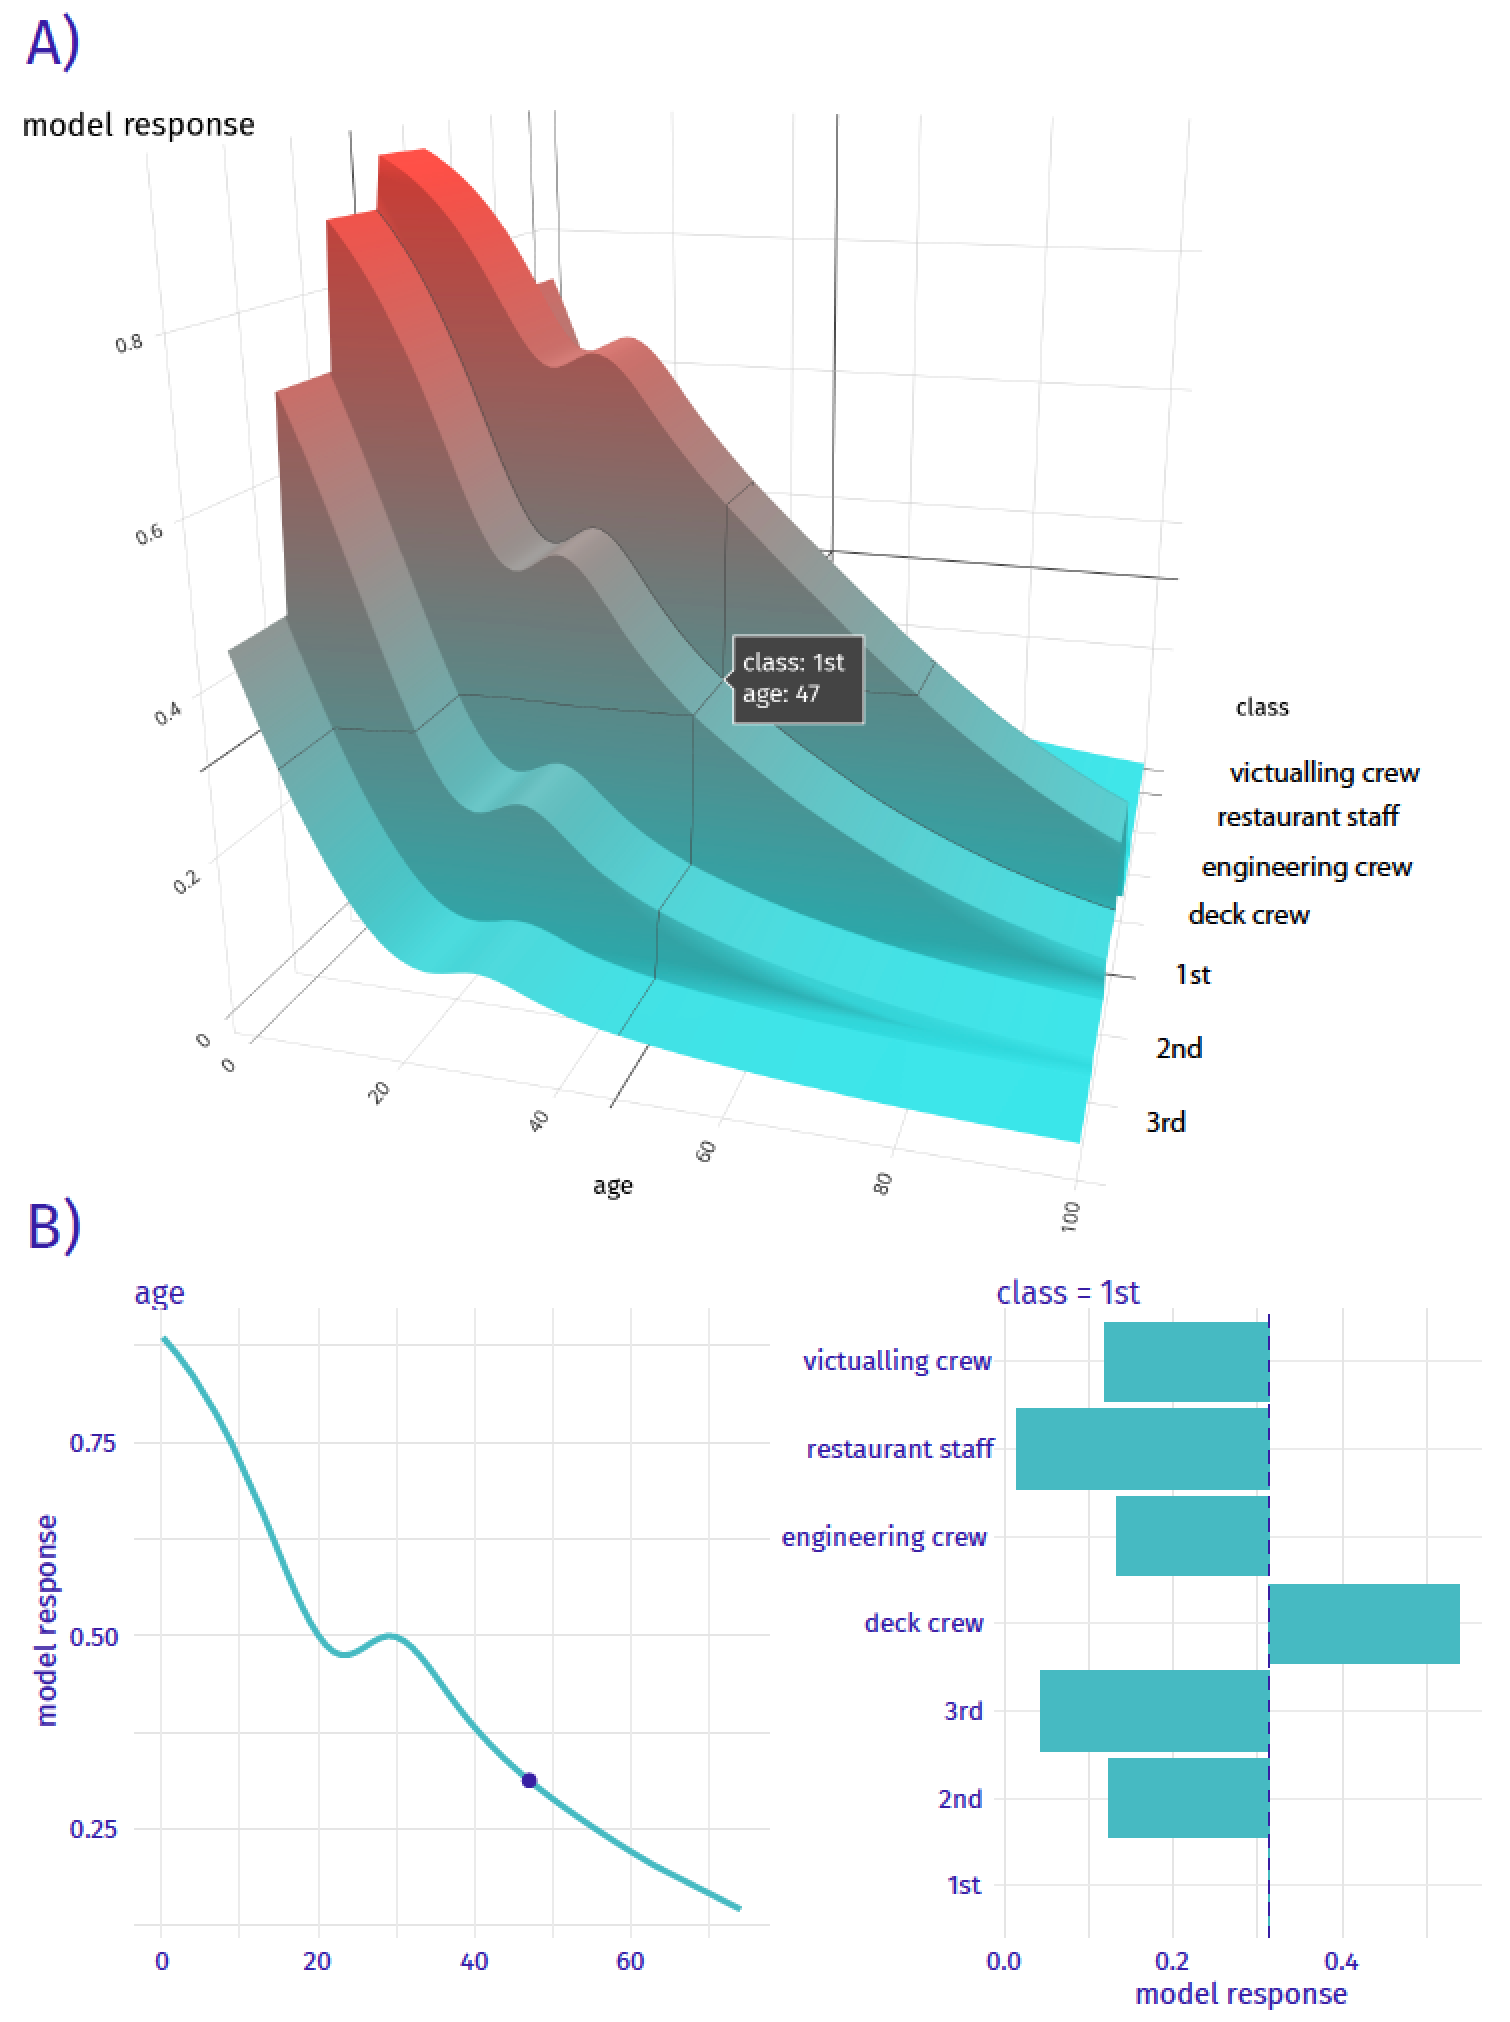
\includegraphics[width=0.7\linewidth]{figure/profile_age_class} 

}

\caption{(fig:modelResponseCurveLine) A) Model response (prediction) surface. Ceteris-paribus (CP) profiles marked with black curves help to understand the curvature of the surface while changing only a single explanatory variable. B) CP profiles for individual variables, age (continuous) and class (categorical).}\label{fig:modelResponseCurveLine}
\end{figure}

CP technique is similar to the LIME method (see Chapter \ref{LIME}).
LIME and CP profiles examine the curvature of a model response-surface.
The difference between these two methods lies in the fact that LIME
approximates the black-box model of interest locally with a simpler
white-box model. Usually, the LIME model is sparse, i.e., contains fewer
variables, and thus we have got to graphically investigate a smaller
number of dimensions. On the other hand, the CP profiles present
conditional predictions for every variable and, in most cases, are
easier to intepret.

\hypertarget{method}{%
\subsection{Method}\label{method}}

In this section we introduce more formally uni-dimensional CP profiles.

{[}PBI: Do we need to assume that model is correct? first sentence may
be removed. TOMASZ: ADDED A FEW SENTENCES TO INDICATE THAT THE
APPROXIMATION MAY BE WHATEVER WE WANT.{]}

Assume that \(E_Y(Y | x^*) \approx f(x^*)\), where \(f(x^*)\) is the
value of the model at \(x^*\), where \(x^*\) is a vector containing
values for explanatory covariates. Note that we do not require the
approximation to be ``good'' in any particular sense; we simply assume
that we have got a model that is used to estimate the expected value and
provide predictions of the dependent variable. Our interest lies in the
evalution of the quality of the predictions. If the model offers a
``good'' approximation of the expected value, it should be reflected in
its satisfactory predictive performance.

We will use subscript \(x^*_i\) to refer to the vector corresponding to
the \(i\)-th observation in a dataset. We will use superscript
\(x^{*j}\) to refer to the \(j\)-th element of \(x^*\), i.e., the
\(j\)-th variable. Additionally, let \(x^{*-j}\) denote a vector
resultinig from removing the \(j\)-th element from vector \(x^{*}\).
Moreover, let \(x^{*|j}=z\) denotes a vector in which the \(j\)-th
element is equal to \(z\) (a scalar).

We define a one-dimensional CP profile for the model \(f()\), \(j\)-th
explanatory variable, and point \(x^*\) as follows:

\[
CP^{f, j, x^*}(z) \equiv f(x^{*|j} = z).
\] That is, CP profile is a function that provides the dependence of the
(approximate) expected value (prediction) of the model for \(Y\) on the
value of \(j\)-th explanatory variable \(z\), where \(z\) is taken to go
through the range of values typical for the variable and values of all
other variables in \(x^*\) are kept fixed at the values present in
\(x^*\).

For continuous explanatory variables a natural way to represent the CP
function is to use a profile plot similar to the ones presented in
Figure \ref{fig:profileAgeRf}. In the figure, the dot on the curves
marks an instance prediction, i.e., prediction \(f(x^*)\) for a single
observation \(x^*\). The curve itself shows how the prediction would
change if the value of a particular explanatory variable changed. Figure
\ref{fig:profileAgeRf} presents CP profiles for the \emph{age} variable
in the logistic regression and random forest models for the Titanic
dataset (see Section \ref{HFDataset}). It is worth oberving that the
profile for the logistic regression model is smooth, while for the
random forest model it shows more variability. Moreover, for this
instance (observation), the prediction would increase substantially if
the value of the explanatory variable became lower than 20.

\textbackslash{}begin\{figure\}

\{\centering 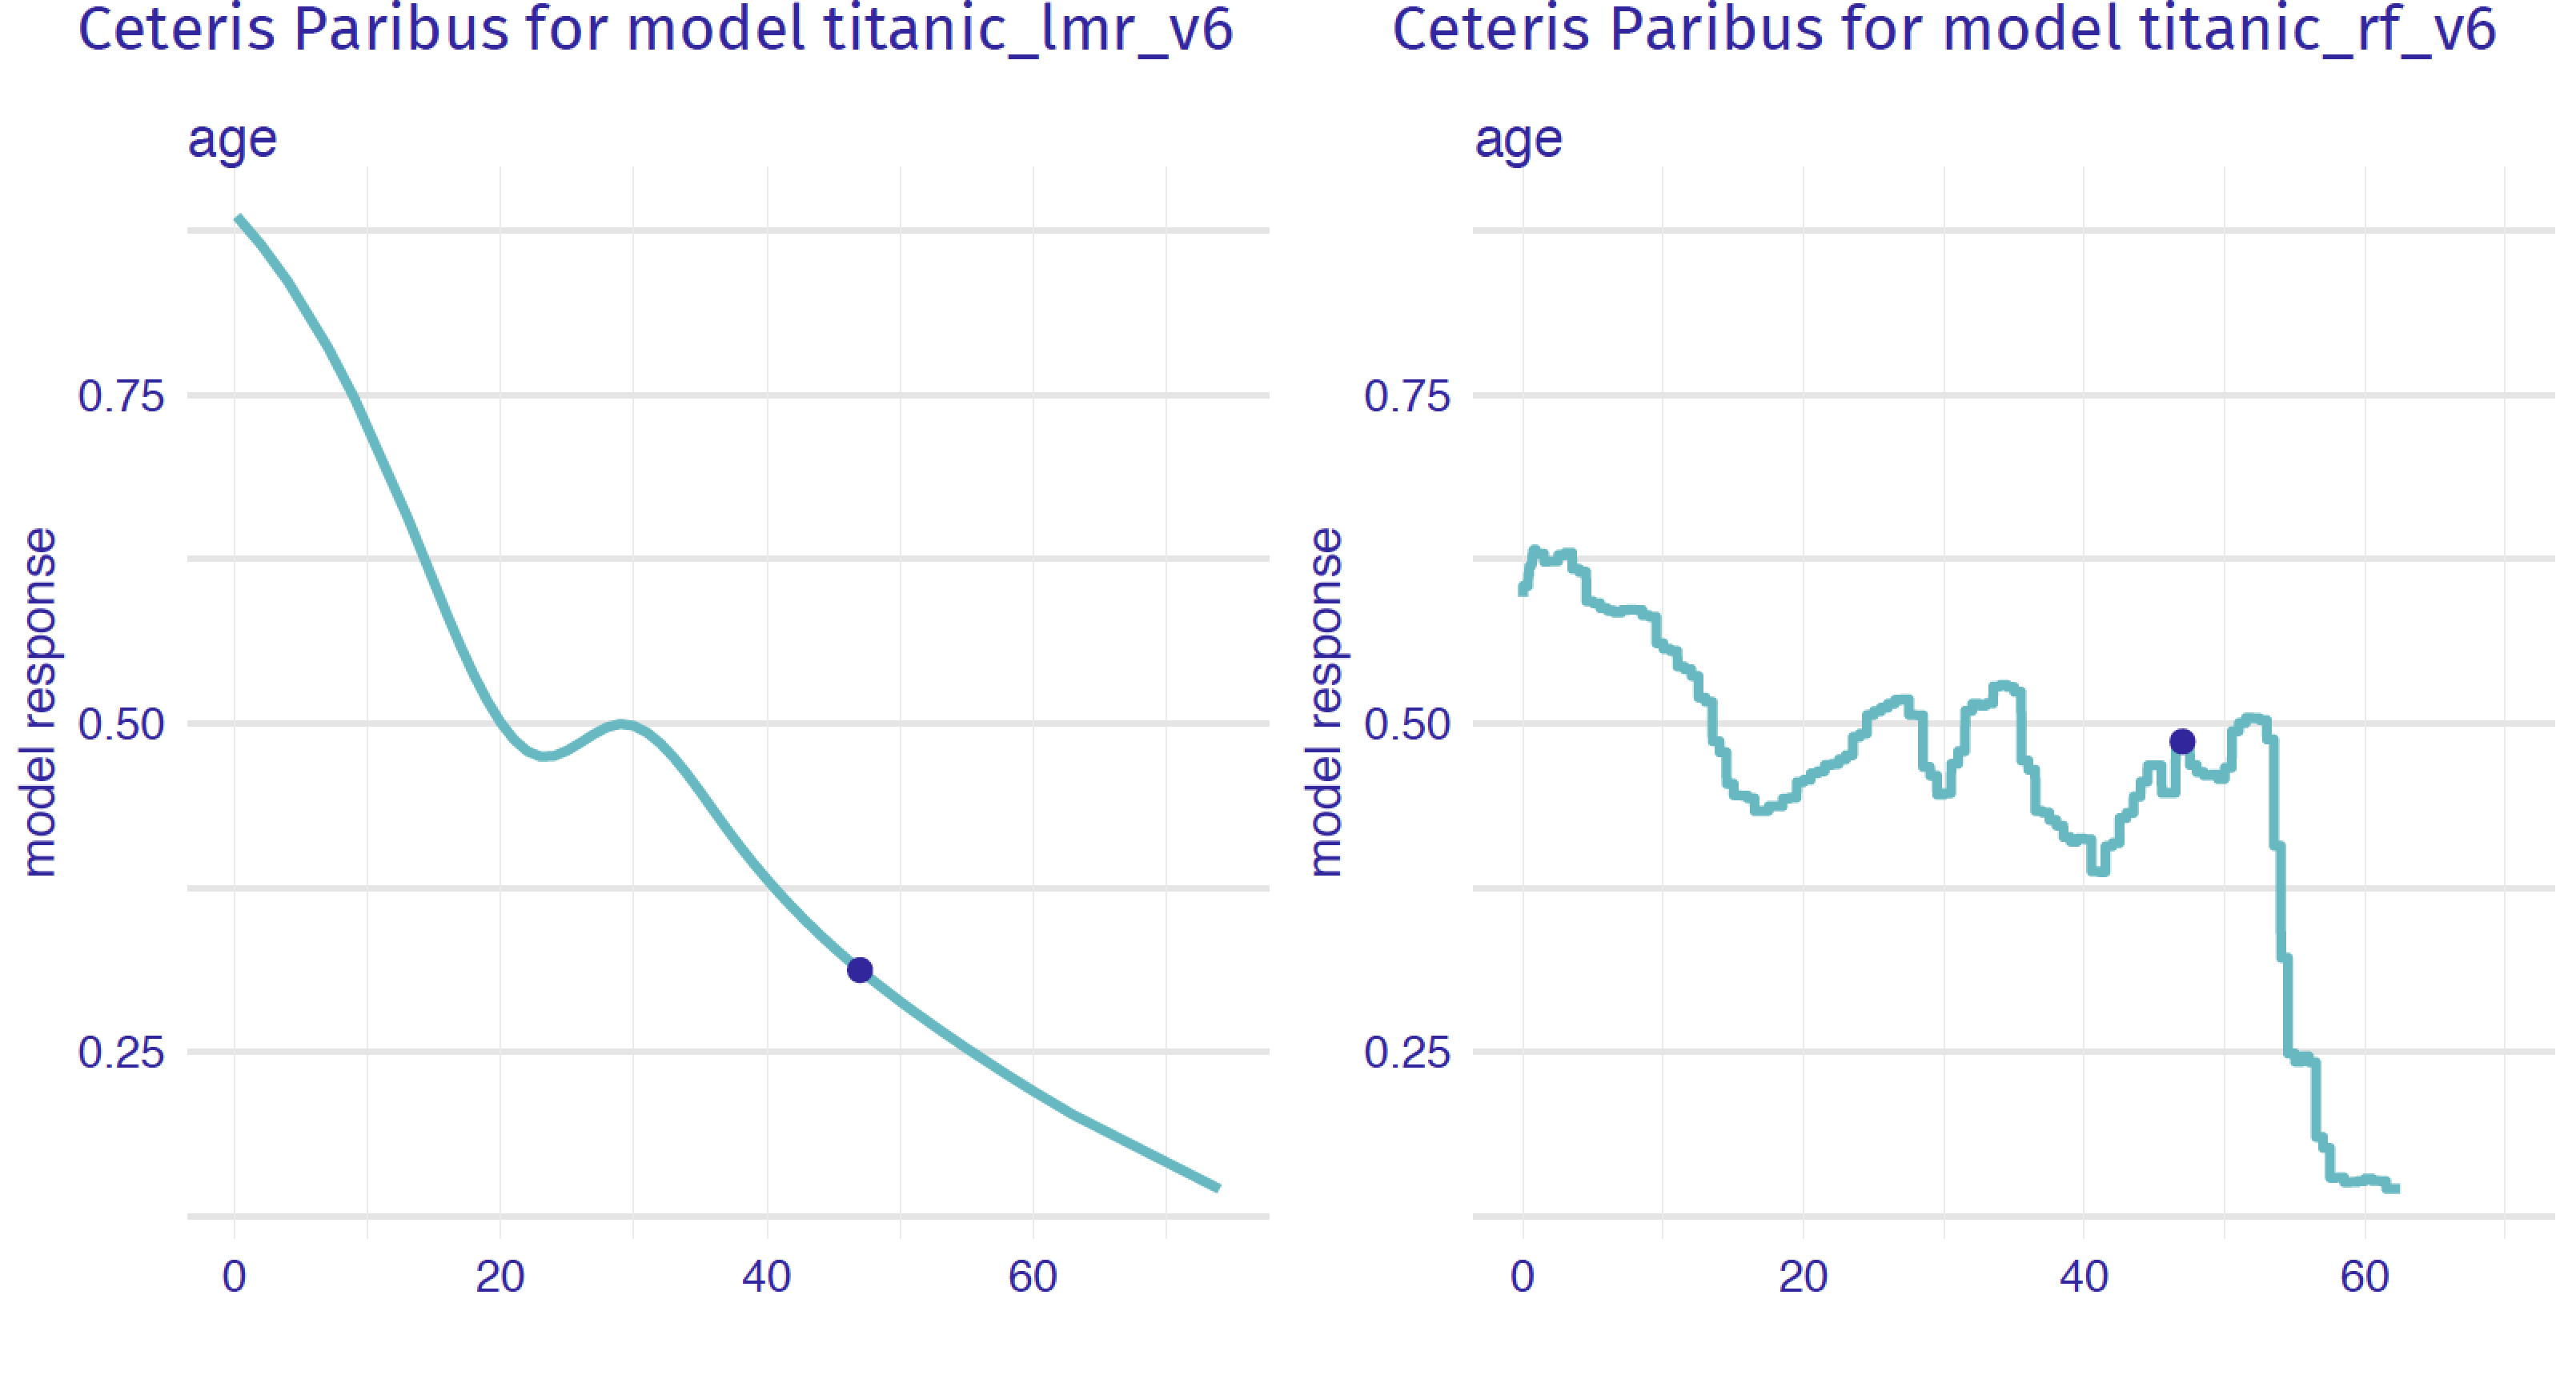
\includegraphics[width=0.7\linewidth]{figure/profile_age_rf}

\}

\textbackslash{}caption\{(fig:profileAgeRf) Ceteris-paribus profiles for
variable \texttt{age} for the logistic regression
(\texttt{titanic\_lmr\_v6}) and random forest (\texttt{titanic\_rf\_v6}
) models that predict the probability of surviving based on the Titanic
data\}\label{fig:profileAgeRf} \textbackslash{}end\{figure\}

For a categorical explanatory variable, a natural way to represent the
CP function is to use a barplot similar to the ones presented in Figure
\ref{fig:profileAgeRf2}.

\textbackslash{}begin\{figure\}

\{\centering 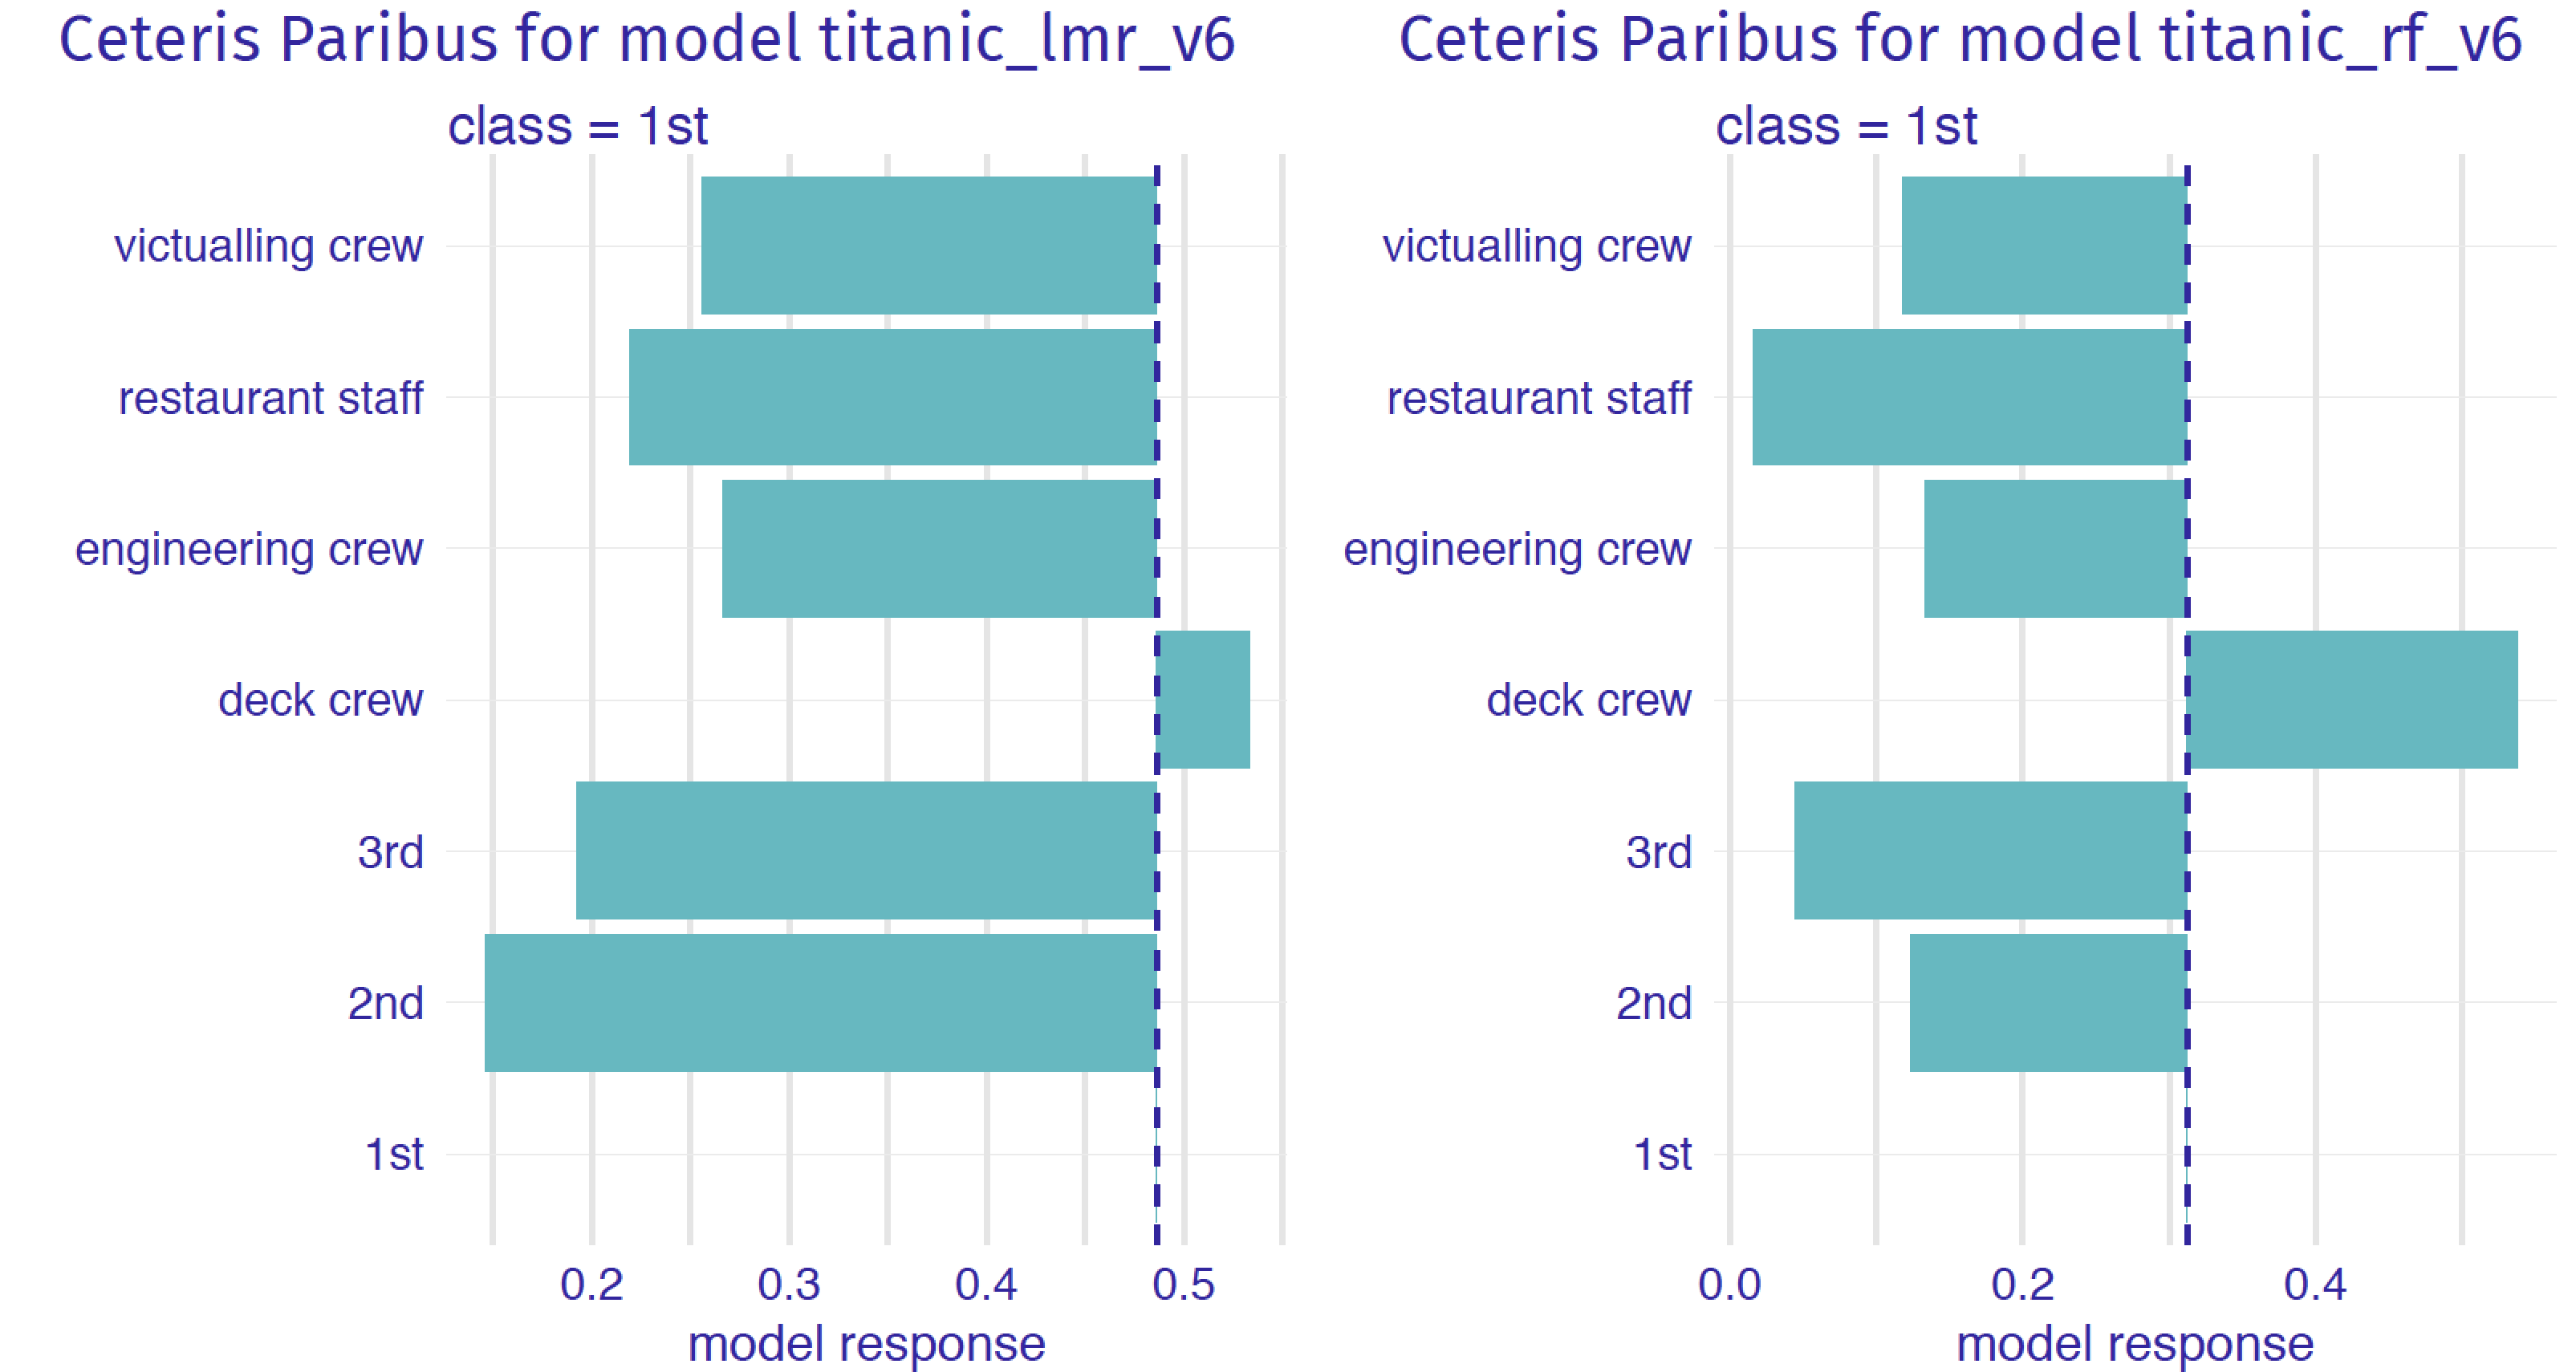
\includegraphics[width=0.7\linewidth]{figure/profile_class_rf}

\}

\textbackslash{}caption\{(fig:profileAgeRf2) Ceteris-paribus profiles
for variable \texttt{class} for the logistic regression
(\texttt{titanic\_lmr\_v6}) and random forest (\texttt{titanic\_rf\_v6}
) models that predict the probability of surviving based on the Titanic
data\}\label{fig:profileAgeRf2} \textbackslash{}end\{figure\}

Usually, black-box models contain a large number of explanatory
variables. However, CP profiles are legible even for tiny subplots,
created with techniques like sparklines or small multiples
\citep{Tufte1986}. In this way we can display a large number of profiles
at the same time keeping profiles for consecutive variables in separate
panels, as shown in Figure \ref{fig:profileV4Rf}. It helps if these
panels are ordered so that the most important profiles are listed first.
We discuss a method to assess importance of CP profiles in the next
chapter.

\textbackslash{}begin\{figure\}

\{\centering 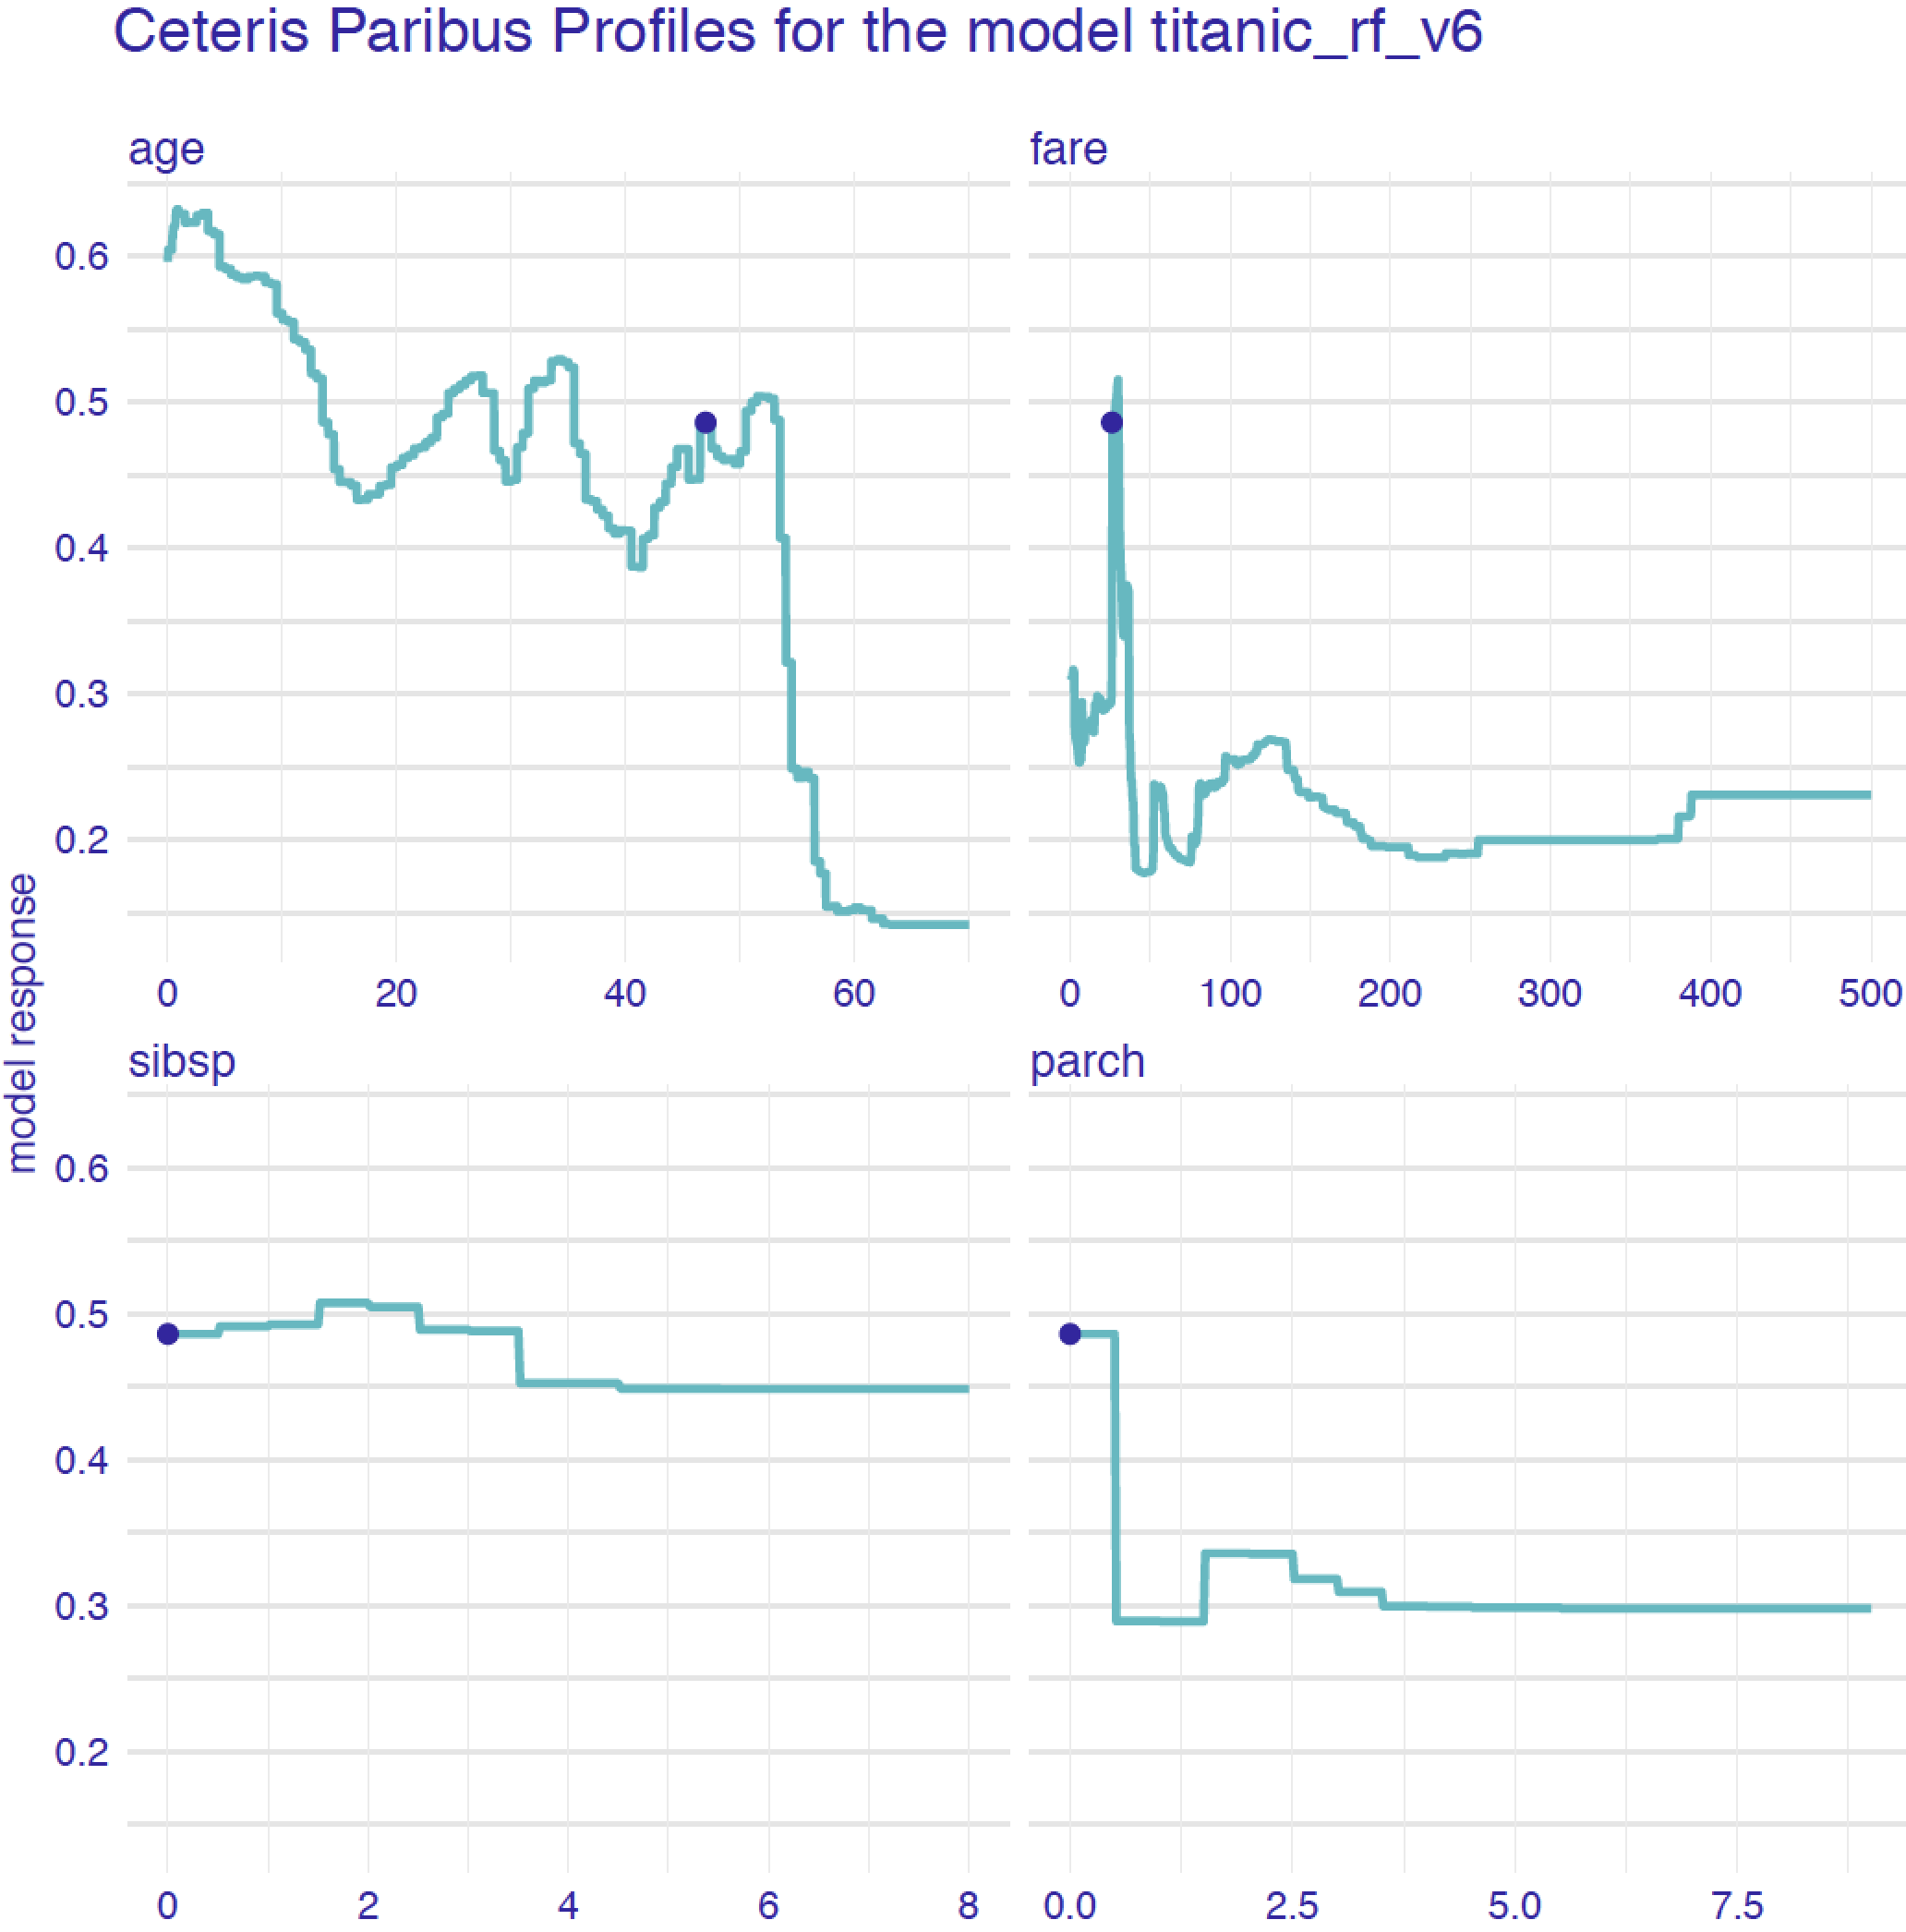
\includegraphics[width=0.7\linewidth]{figure/profile_v4_rf}

\}

\textbackslash{}caption\{(fig:profileV4Rf) Ceteris-paribus profiles for
all continuous explanatory variables for the random forest
(\texttt{titanic\_rf\_v6}) model for the \texttt{titanic}
dataset\}\label{fig:profileV4Rf} \textbackslash{}end\{figure\}

\hypertarget{pros-and-cons}{%
\subsection{Pros and cons}\label{pros-and-cons}}

One-dimensional CP profiles,as presented in this chapter, offer a
uniform, easy to comunicate and extendable approach to model
exploration. Their graphical representation is easy to understand and
explain. It is possible to show profiles for many variables or models in
a single plot.

There are several issues related to the use of the CP profiles. If
explanatory variables are correlated, then changing one variable implies
a change in the other. In such case, the application of the
\emph{Ceteris paribus} principle may lead to unrealistic settings, as it
is not possible to keep one variable fixed while changing the other one.
A special case are interactions, which require the use of
two-dimensional CP profiles that are more complex than one-dimensional
ones. Also, in case of a model with hundreds or thousands of variables,
the number of plots to inspect may be daunting. Finally, while barplots
allow visualization of CP profiles for factors (categorical explanatory
variables), their use becomes less trivial in case of factors with many
nominal (unordered) categories (like, for example, a ZIP-code).

\hypertarget{code-snippets-for-r}{%
\subsection{Code snippets for R}\label{code-snippets-for-r}}

In this section we present key features of the R package
\texttt{ingredients} \citep{ingredientsRPackage} which is a part of
\texttt{DALEXverse} and covers all methods presented in this chapter.
More details and examples can be found at
\texttt{https://modeloriented.github.io/ingredients/}.

Note that there are also other R packages that offer similar
functionality, like \texttt{condvis} \citep{JSSv081i05}, \texttt{pdp}
\citep{pdpRPackage}, \texttt{ICEbox} \citep{ICEboxRPackage},
\texttt{ALEPlot} \citep{ALEPlotRPackage}, \texttt{iml}
\citep{imlRPackage}.

In this section we use the random forest \citep{R-randomForest} model
developed for the Titanic dataset (see Section \ref{TitanicDataset}). In
particular, we deal with a binary classification problem - we want to
predict the probability of survival for a selected passenger.

{[}TOMASZ: SHOULD WE NOT RE-USE THE \texttt{titanic\_rf\_v6} OBJECT?
ALSO, HOW ABOUT MISSING DATA IMPUTATION USED EARLIER?{]}

\begin{Shaded}
\begin{Highlighting}[]
\KeywordTok{library}\NormalTok{(}\StringTok{"DALEX"}\NormalTok{)}
\NormalTok{titanic <-}\StringTok{ }\KeywordTok{na.omit}\NormalTok{(titanic)}
\KeywordTok{head}\NormalTok{(titanic, }\DecValTok{2}\NormalTok{)}
\end{Highlighting}
\end{Shaded}

\begin{verbatim}
##   gender age class    embarked       country  fare sibsp parch survived
## 1   male  42   3rd Southampton United States  7.11     0     0       no
## 2   male  13   3rd Southampton United States 20.05     0     2       no
##   age_cat fare_cat
## 1 (30,50]   (0,10]
## 2 (10,18]  (10,25]
\end{verbatim}

\begin{Shaded}
\begin{Highlighting}[]
\KeywordTok{library}\NormalTok{(}\StringTok{"randomForest"}\NormalTok{)}
\NormalTok{model_titanic_rf <-}\StringTok{ }\KeywordTok{randomForest}\NormalTok{(survived }\OperatorTok{==}\StringTok{ "yes"} \OperatorTok{~}\StringTok{ }\NormalTok{gender }\OperatorTok{+}\StringTok{ }\NormalTok{age }\OperatorTok{+}\StringTok{ }\NormalTok{class }\OperatorTok{+}\StringTok{ }\NormalTok{embarked }\OperatorTok{+}
\StringTok{                                   }\NormalTok{fare }\OperatorTok{+}\StringTok{ }\NormalTok{sibsp }\OperatorTok{+}\StringTok{ }\NormalTok{parch,  }\DataTypeTok{data =}\NormalTok{ titanic)}
\end{Highlighting}
\end{Shaded}

CP profiles are calculated in four steps with the \texttt{ingredients}
package.

\textbf{1. Create an explainer - wrapper around model and validation
data.}

Model-objects created with different libraries may have different
internal structures. Thus, first, we have got to create a wrapper around
the model. Toward this end, we use the \texttt{explain()} function from
the \texttt{DALEX} package \citep{R-DALEX}. The function requires five
arguments:

\begin{itemize}
\tightlist
\item
  \texttt{model} a model-object,
\item
  \texttt{data} a validation data frame,
\item
  \texttt{y} observed values of the dependent variable for the
  validation data,
\item
  \texttt{predict\_function} a function that returns prediction scores,
  if not specified, then a default \texttt{predict()} function is used.
\item
  \texttt{label} a function that returns prediction scores, if not
  specified then it is extracted from the \texttt{class(model)}.
\end{itemize}

In the example below we use the training data as the validation dataset.

\begin{Shaded}
\begin{Highlighting}[]
\NormalTok{explain_titanic_rf <-}\StringTok{ }\KeywordTok{explain}\NormalTok{(}\DataTypeTok{model =}\NormalTok{ model_titanic_rf, }
                              \DataTypeTok{data =}\NormalTok{ titanic[,}\OperatorTok{-}\DecValTok{9}\NormalTok{],}
                              \DataTypeTok{y =}\NormalTok{ titanic}\OperatorTok{$}\NormalTok{survived }\OperatorTok{==}\StringTok{ "yes"}\NormalTok{, }
                              \DataTypeTok{label =} \StringTok{"Random Forest v7"}\NormalTok{)}
\end{Highlighting}
\end{Shaded}

\textbf{2. Define the instance (observation) of interest.}

CP profiles explore model around a single observation. Thus, in the
exampe below, we define data frame \texttt{johny\_d} with a single row.
It describes an 8-years old boy that travels in the first class without
parents and siblings. Then, we obtain the model prediction for this
instance with the help of the `predict()' function. In particular, we
compute the probability for each category of the dependent binary
variable.

{[}TOMASZ: IN THE DATA CHAPTER WE HAD DATA FRAME HENRY. SHOULD NOT WE
RE-USE IT HERE?{]}

\begin{Shaded}
\begin{Highlighting}[]
\NormalTok{johny_d <-}\StringTok{ }\KeywordTok{data.frame}\NormalTok{(}
  \DataTypeTok{class =} \KeywordTok{factor}\NormalTok{(}\StringTok{"1st"}\NormalTok{, }\DataTypeTok{levels =} \KeywordTok{c}\NormalTok{(}\StringTok{"1st"}\NormalTok{, }\StringTok{"2nd"}\NormalTok{, }\StringTok{"3rd"}\NormalTok{, }\StringTok{"deck crew"}\NormalTok{, }\StringTok{"engineering crew"}\NormalTok{, }
                                  \StringTok{"restaurant staff"}\NormalTok{, }\StringTok{"victualling crew"}\NormalTok{)),}
  \DataTypeTok{gender =} \KeywordTok{factor}\NormalTok{(}\StringTok{"male"}\NormalTok{, }\DataTypeTok{levels =} \KeywordTok{c}\NormalTok{(}\StringTok{"female"}\NormalTok{, }\StringTok{"male"}\NormalTok{)),}
  \DataTypeTok{age =} \DecValTok{8}\NormalTok{,}
  \DataTypeTok{sibsp =} \DecValTok{0}\NormalTok{,}
  \DataTypeTok{parch =} \DecValTok{0}\NormalTok{,}
  \DataTypeTok{fare =} \DecValTok{72}\NormalTok{,}
  \DataTypeTok{embarked =} \KeywordTok{factor}\NormalTok{(}\StringTok{"Southampton"}\NormalTok{, }\DataTypeTok{levels =} \KeywordTok{c}\NormalTok{(}\StringTok{"Belfast"}\NormalTok{, }\StringTok{"Cherbourg"}\NormalTok{, }\StringTok{"Queenstown"}\NormalTok{, }\StringTok{"Southampton"}\NormalTok{))}
\NormalTok{)}

\KeywordTok{predict}\NormalTok{(explain_titanic_rf, johny_d)}
\end{Highlighting}
\end{Shaded}

\begin{verbatim}
##         1 
## 0.4555335
\end{verbatim}

\textbf{3. Calculate CP profiles}

To obtain CP profiles, we use the \texttt{ceteris\_paribus()} function.
It requires the explainer-object and the instance data frame as
arguments. By default, CP profiles are calculated for all numerical
variables. To select a subset of variables, the \texttt{variables}
argument can be used.

As a result, the function yields an object od the class
\texttt{ceteris\_paribus\_explainer}. It is a data frame with model
predictions.

\begin{Shaded}
\begin{Highlighting}[]
\KeywordTok{library}\NormalTok{(}\StringTok{"ingredients"}\NormalTok{)}
\NormalTok{cp_titanic_rf <-}\StringTok{ }\KeywordTok{ceteris_paribus}\NormalTok{(explain_titanic_rf, johny_d, }
                            \DataTypeTok{variables =} \KeywordTok{c}\NormalTok{(}\StringTok{"age"}\NormalTok{, }\StringTok{"fare"}\NormalTok{, }\StringTok{"class"}\NormalTok{, }\StringTok{"gender"}\NormalTok{))}
\NormalTok{cp_titanic_rf}
\end{Highlighting}
\end{Shaded}

\begin{verbatim}
## Top profiles    : 
##     class gender        age sibsp parch fare    embarked    _yhat_ _vname_
## 1     1st   male  0.1666667     0     0   72 Southampton 0.4817883     age
## 1.1   1st   male  2.0000000     0     0   72 Southampton 0.4905560     age
## 1.2   1st   male  4.0000000     0     0   72 Southampton 0.4901385     age
## 1.3   1st   male  7.0000000     0     0   72 Southampton 0.4582002     age
## 1.4   1st   male 10.0000000     0     0   72 Southampton 0.4251985     age
## 1.5   1st   male 14.0000000     0     0   72 Southampton 0.3070365     age
##     _ids_          _label_
## 1       1 Random Forest v7
## 1.1     1 Random Forest v7
## 1.2     1 Random Forest v7
## 1.3     1 Random Forest v7
## 1.4     1 Random Forest v7
## 1.5     1 Random Forest v7
## 
## 
## Top observations:
##   class gender age sibsp parch fare    embarked    _yhat_          _label_
## 1   1st   male   8     0     0   72 Southampton 0.4555335 Random Forest v7
##   _ids_
## 1     1
\end{verbatim}

\textbf{4. Plot CP profiles.}

To obtain a graphical represenation of CP profiles, the generic
\texttt{plot()} function can be applied to the data frame returend by
the \texttt{ceteris\_paribus()} function. It returns a \texttt{ggplot2}
object that can be processed if needed.

The resulting plot can be enriched with additional data by applying
functions \texttt{show\_rugs} (adds rugs for the selected points),
\texttt{show\_observations} (adds observations), or
\texttt{show\_aggreagated\_profiles} (see Chapter
\ref{variableEngeneering}). All these functions can take additional
arguments to modify size, color, or linetype.

\begin{Shaded}
\begin{Highlighting}[]
\KeywordTok{library}\NormalTok{(}\StringTok{"ggplot2"}\NormalTok{)}
\KeywordTok{plot}\NormalTok{(cp_titanic_rf) }\OperatorTok{+}
\StringTok{  }\KeywordTok{show_observations}\NormalTok{(cp_titanic_rf, }\DataTypeTok{variables =} \KeywordTok{c}\NormalTok{(}\StringTok{"age"}\NormalTok{, }\StringTok{"fare"}\NormalTok{)) }\OperatorTok{+}
\StringTok{  }\KeywordTok{ggtitle}\NormalTok{(}\StringTok{"Ceteris Paribus Profiles"}\NormalTok{, }\StringTok{"For the random forest model and titanic dataset"}\NormalTok{)}
\end{Highlighting}
\end{Shaded}

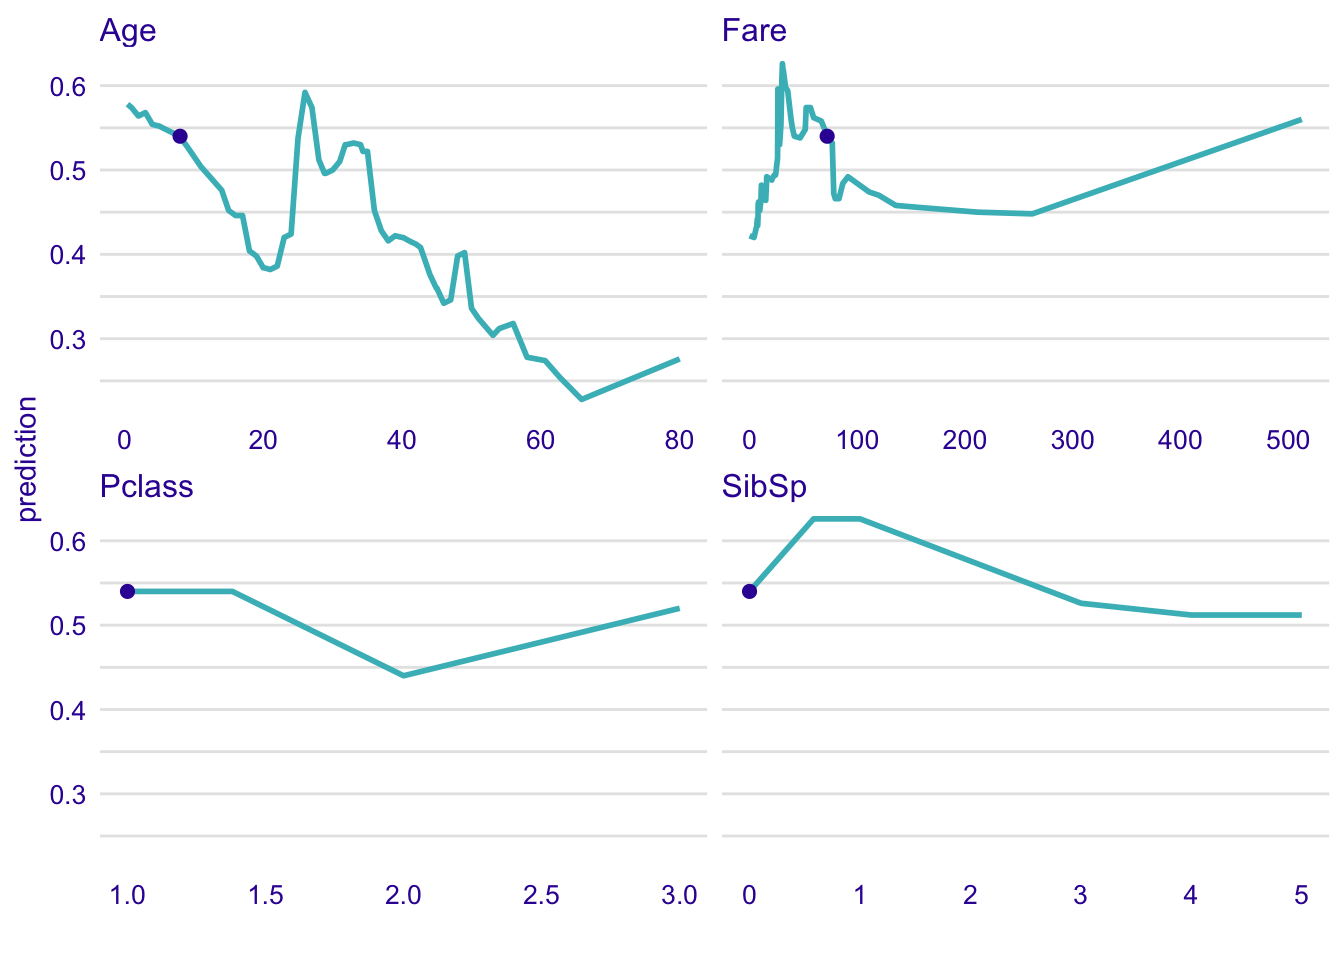
\includegraphics{PM_VEE_files/figure-latex/unnamed-chunk-22-1.pdf}

\hypertarget{ceterisParibusOscillations}{%
\section{Ceteris Paribus Oscillations - a tool for local variable
importance}\label{ceterisParibusOscillations}}

\hypertarget{introduction-2}{%
\subsection{Introduction}\label{introduction-2}}

Visual examination of Ceteris Paribus Profiles is insightful, but for a
model with a large number of explanatory variables we may end up with a
large number of plots which may be overwhelming. To prioritize between
profiles we need a measure that would summarize the impact of a selected
variable on model's predictions. We will propose now a solution closely
linked with CP profiles, but the issue is also discussed also in the
next chapter.

\hypertarget{intuition-1}{%
\subsection{Intuition}\label{intuition-1}}

To assign importance to CP profiles, we can use the concept of profile
oscillations. In particular, the larger influence of an explanatory
variable on prediction at a particular instance, the larger the
fluctuations along the corresponding CP profile. For a variable that
exercises little or no influence on model prediction, the profile will
be flat or will barely change. Figure \ref{fig:CPVIPprofiles}
illustrates the idea behind measuring oscillations. The larger the
highlighted area, the more important is the variable.

\textbackslash{}begin\{figure\}

\{\centering 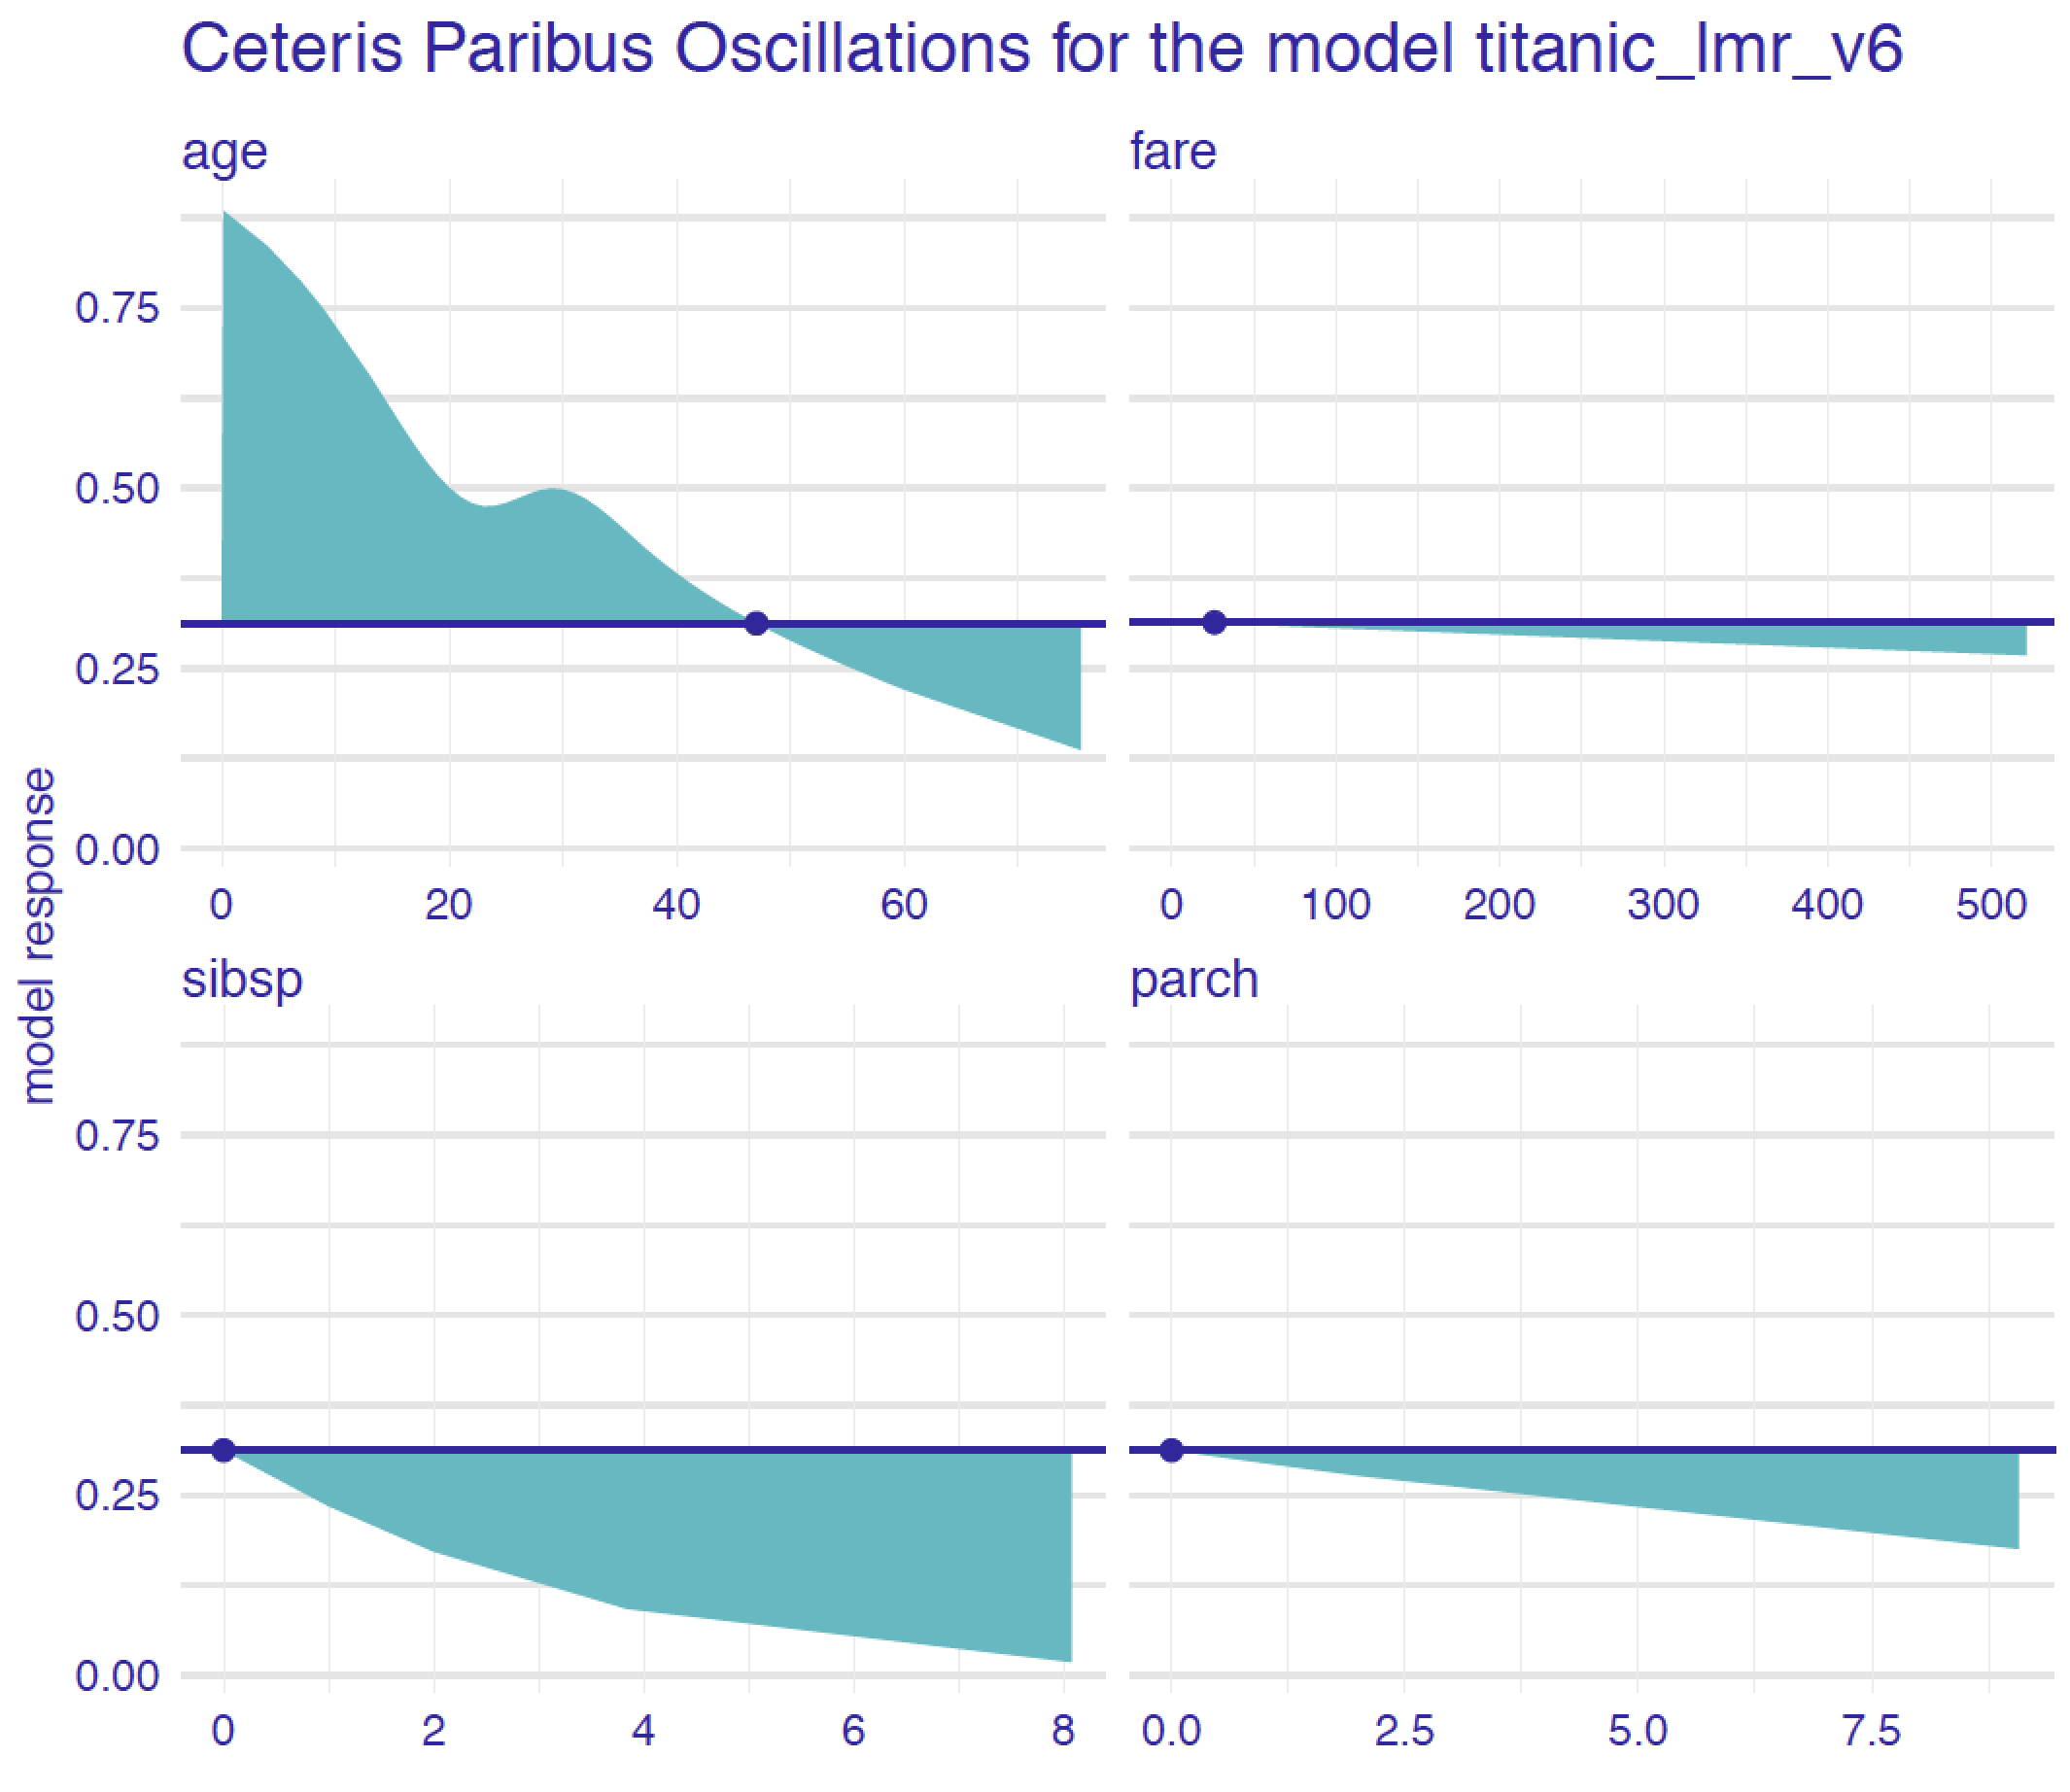
\includegraphics[width=0.7\linewidth]{figure/oscillations_all_lmr}

\}

\textbackslash{}caption\{(fig:CPVIPprofiles) The value of the red are
area summarizes CP oscillations and provides the average absolute
deviations between the CP profile and the instance prediction. This
example is for the \texttt{titanic\_lmer\_v6} model and the
\texttt{titanic} dataset\}\label{fig:CPVIPprofiles}
\textbackslash{}end\{figure\}

Figure \ref{fig:CPVIP1} provides a plot of variable importance measures
for different variables for the \texttt{titanic\_lmer\_v6} and the
\texttt{titanic} dataset. The wider the interval, the larger the
CP-profile oscillations for a particular explanatory variable. Thus,
Figure \ref{fig:CPVIP1} indicates that the most important variable for
prediction for a selected observation is \texttt{age}, followed by
\texttt{sibsp}.

\textbackslash{}begin\{figure\}

\{\centering 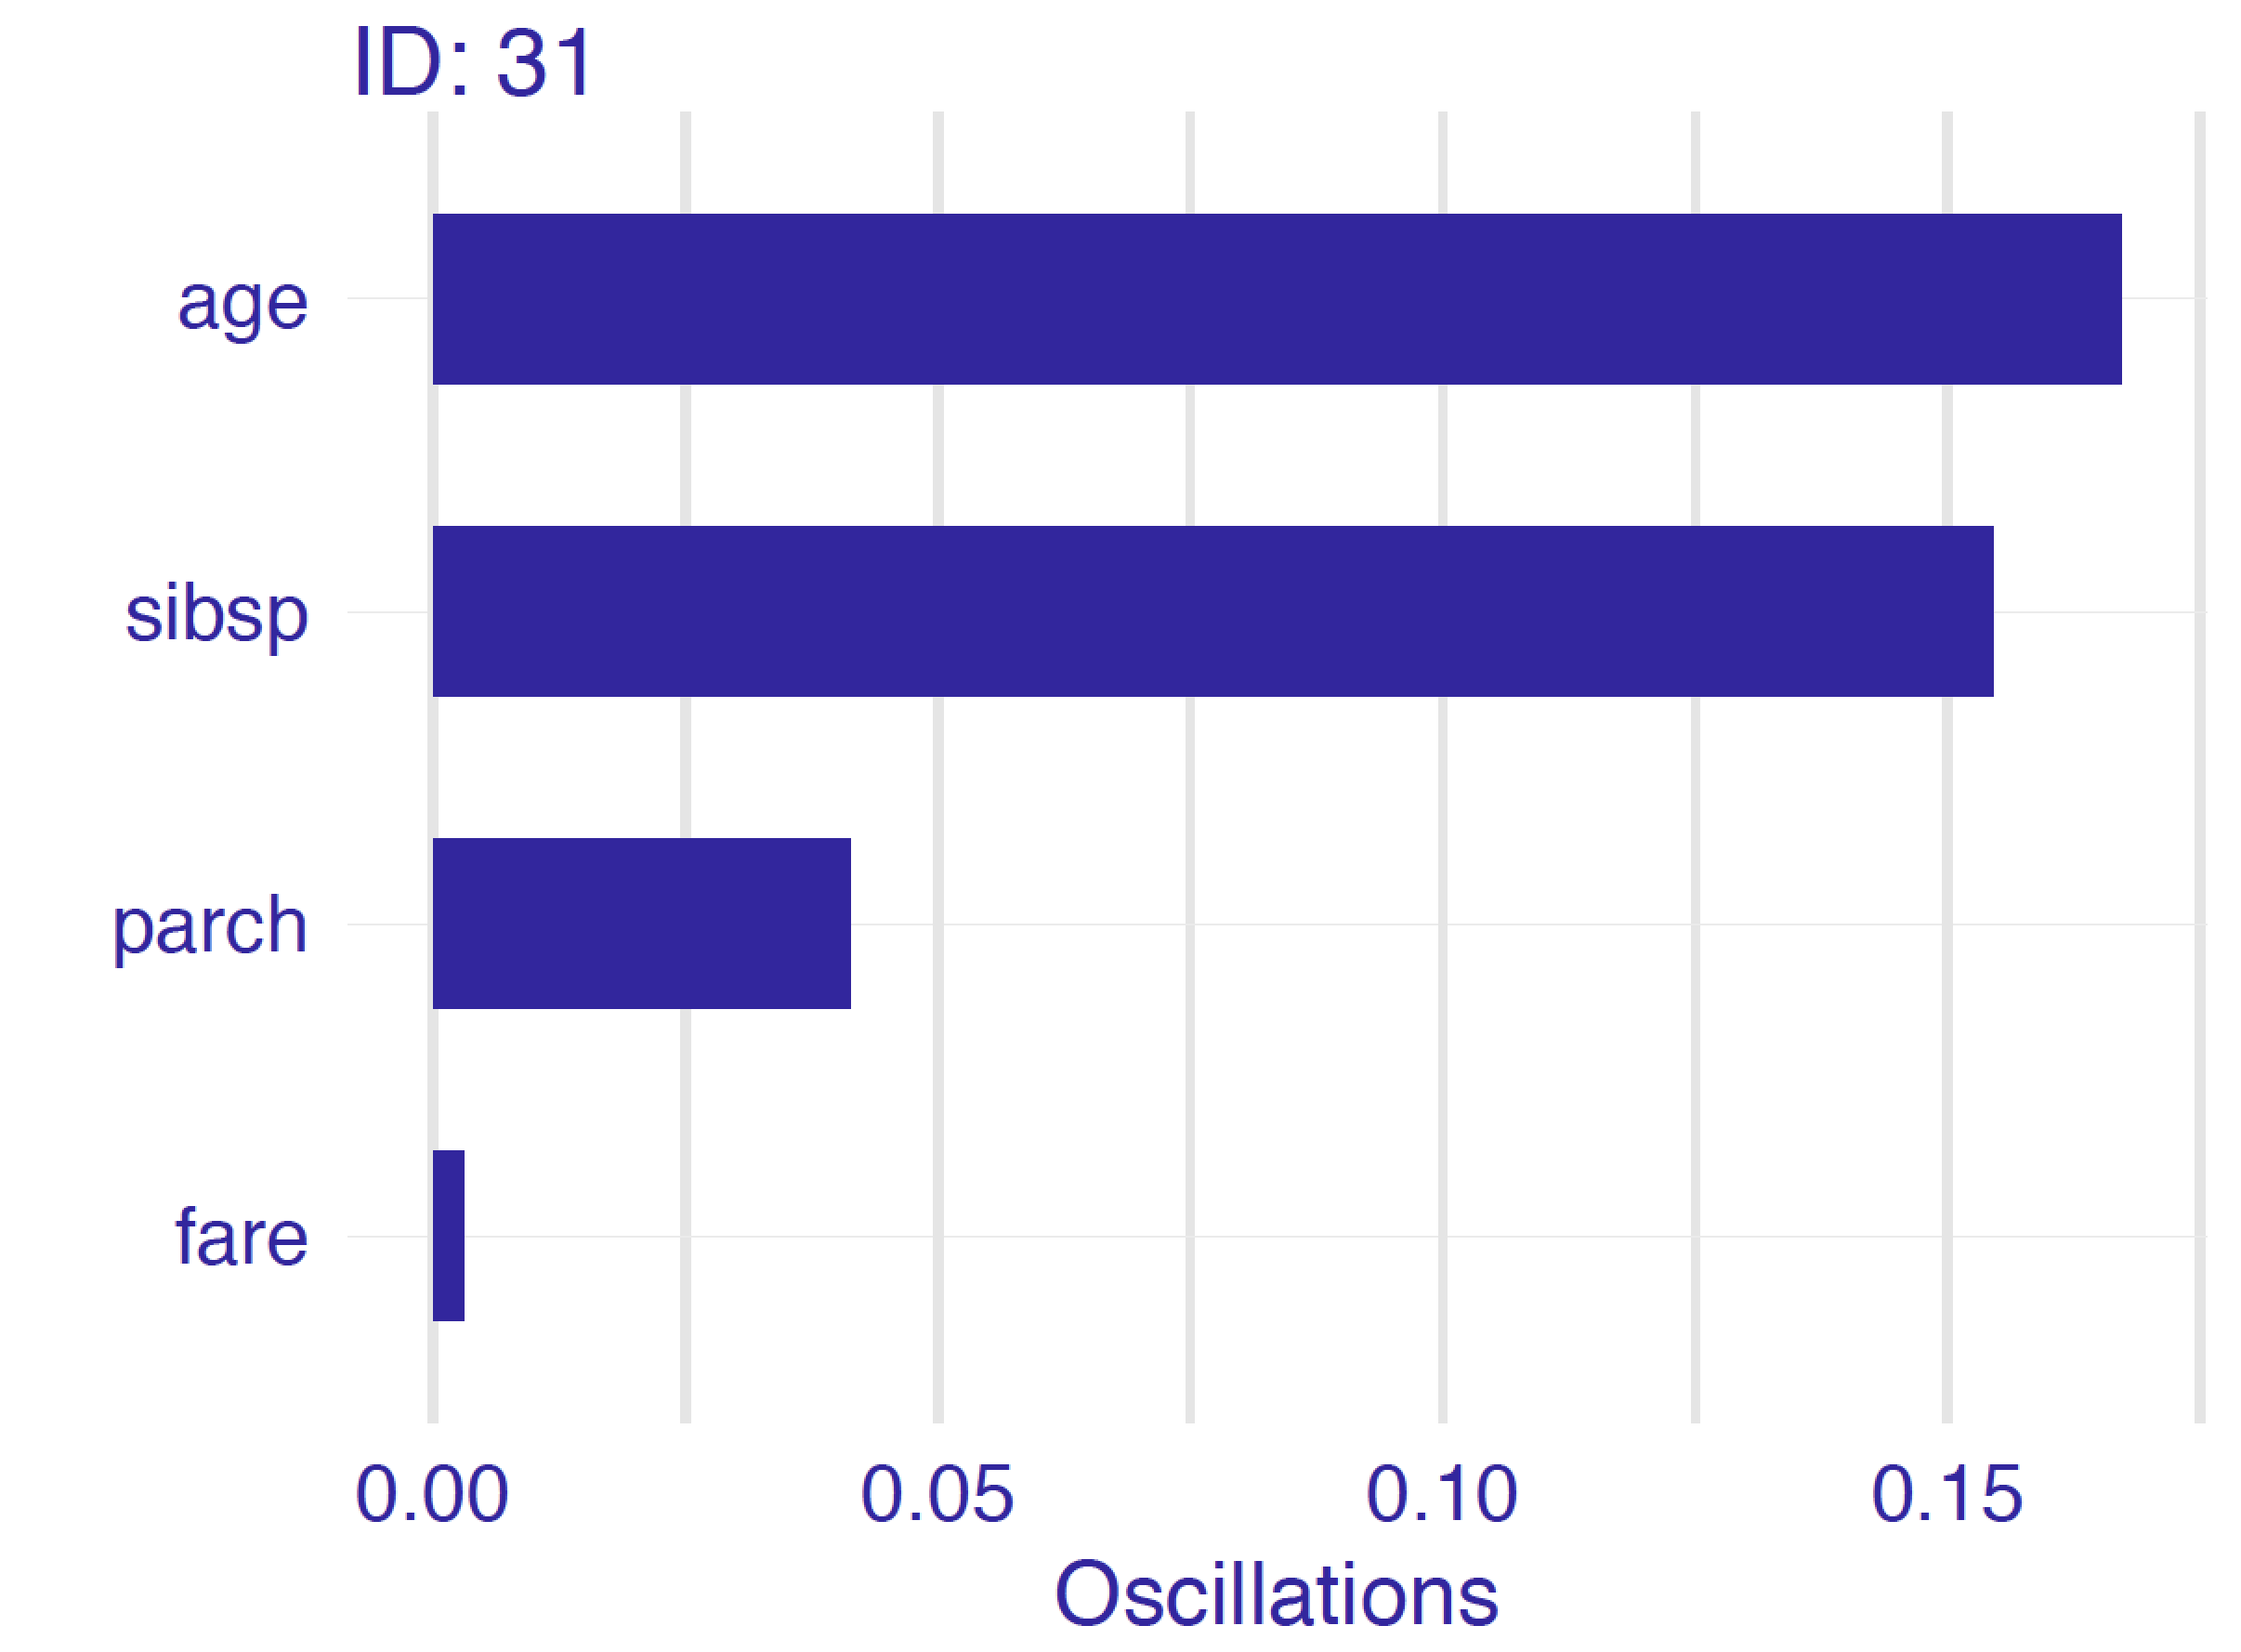
\includegraphics[width=0.5\linewidth]{figure/oscillations_all_lmr_plot}

\}

\textbackslash{}caption\{(fig:CPVIP1) Variable-importance measures
calculated for Ceteris-paribus oscillations for observation ID: 31. This
example is for the \texttt{titanic\_lmer\_v6} model and the
\texttt{titanic} dataset\}\label{fig:CPVIP1} \textbackslash{}end\{figure\}

\hypertarget{method-1}{%
\subsection{Method}\label{method-1}}

Let us formalize this concept now. Denote by \(g^j(z)\) the probability
density function of the distribution of the \(j\)-th explanatory
variable. The summary measure of the variable's importance for model
prediction at point \(x\), \(vip^{CP}_j(x)\), computed based on the
variable's CP profile, is defined as follows:

\[
vip^{CP}_j(x^*) = \int_{\mathcal R} |CP^{f,j,x^*}(z) - f(x^*)| g^j(z)dz=E_{X_j}[|CP^{f,j,x^*}(X_j) - f(x^*)|].
\] Thus, \(vip^{CP}_j(x^*)\) is the expected absolute deviation of the
CP profile from the model prediction for \(x^*\) over the distribution
of the \(j\)-th explanatory variable. A straightforward estimator of
\(vip^{CP}_j(x^*)\) is

\[
\widehat{ vip^{CP}_j(x^*)} = \frac 1n \sum_{i=1}^n |CP^{f,j,x^*}(x^{*j}_i) - f(x^*)|,
\] where index \(i\) goes through all observations in a dataset.

Note that the importance of an explanatory variable for instance
prediction may be very different for different points \(x^*\). For
example, consider model \[
f(x_1, x_2) = x_1 * x_2,
\] where \(x_1\) and \(x_2\) take values in \([0,1]\). Consider
prediction for an observation described by vector \(x^* = (0,1)\). In
that case, the importance of \(X_1\) is larger than \(X_2\). This is
because the CP profile for the first variable, given by the values of
function \(f(z,1)=z\), will have oscillations, while the profile for the
second variable will show no oscillation, because it is given by
function \(f(0,z)=0\). Obviously, the situation is reversed for
\(x^*=(1,0)\).

\hypertarget{pros-and-cons-1}{%
\subsection{Pros and cons}\label{pros-and-cons-1}}

By using oscillations of Ceteris Paribus profiles it is possible to
select the most important variables for a single instance. The
methodology is easy to extend to two or more variables. Oscillations are
easy to interpret.

There are several issues related to the use of the CP oscillations. Two
most serious are:

\begin{itemize}
\tightlist
\item
  if two variables are correlated, then Ceteris Paribus profiles may be
  misleading as they do not take correlations into account.
\item
  local feature importance do not sum up to model prediction. In next
  sections we will introduce variable attribution measures that
  eliminate this problem.
\end{itemize}

\hypertarget{code-snippets-for-r-1}{%
\subsection{Code snippets for R}\label{code-snippets-for-r-1}}

In this section we present key features of the R package
\texttt{ingredients} \citep{ingredientsRPackage} which is a part of
\texttt{DALEXverse} and covers all methods presented in this chapter.
More details and examples can be found at
\texttt{https://modeloriented.github.io/ingredients/}.

In this section we use a random forest \citep{R-randomForest} model
\texttt{titanic\_rf\_v6} developed for the Titanic dataset (see Section
\ref{TitanicDataset}). In particular, we deal with a binary
classification problem - we want to predict the probability of survival
for a selected passenger.

\begin{Shaded}
\begin{Highlighting}[]
\KeywordTok{library}\NormalTok{(}\StringTok{"DALEX"}\NormalTok{)}
\KeywordTok{library}\NormalTok{(}\StringTok{"randomForest"}\NormalTok{)}
\NormalTok{titanic <-}\StringTok{ }\KeywordTok{na.omit}\NormalTok{(titanic)}

\NormalTok{model_titanic_rf <-}\StringTok{ }\KeywordTok{randomForest}\NormalTok{(survived }\OperatorTok{==}\StringTok{ "yes"} \OperatorTok{~}\StringTok{ }\NormalTok{gender }\OperatorTok{+}\StringTok{ }\NormalTok{age }\OperatorTok{+}\StringTok{ }\NormalTok{class }\OperatorTok{+}\StringTok{ }\NormalTok{embarked }\OperatorTok{+}
\StringTok{                                   }\NormalTok{fare }\OperatorTok{+}\StringTok{ }\NormalTok{sibsp }\OperatorTok{+}\StringTok{ }\NormalTok{parch,  }\DataTypeTok{data =}\NormalTok{ titanic)}
\NormalTok{explain_titanic_rf <-}\StringTok{ }\KeywordTok{explain}\NormalTok{(}\DataTypeTok{model =}\NormalTok{ model_titanic_rf, }
                              \DataTypeTok{data =}\NormalTok{ titanic[,}\OperatorTok{-}\DecValTok{9}\NormalTok{],}
                              \DataTypeTok{y =}\NormalTok{ titanic}\OperatorTok{$}\NormalTok{survived }\OperatorTok{==}\StringTok{ "yes"}\NormalTok{, }
                              \DataTypeTok{label =} \StringTok{"Random Forest v7"}\NormalTok{)}
\end{Highlighting}
\end{Shaded}

In order to calculate oscillations we need to first calculate Ceteris
Paribus profiles for a selected observation.

Let us use the \texttt{johny\_d} instance again.

\begin{Shaded}
\begin{Highlighting}[]
\NormalTok{johny_d <-}\StringTok{ }\KeywordTok{data.frame}\NormalTok{(}
  \DataTypeTok{class =} \KeywordTok{factor}\NormalTok{(}\StringTok{"1st"}\NormalTok{, }\DataTypeTok{levels =} \KeywordTok{c}\NormalTok{(}\StringTok{"1st"}\NormalTok{, }\StringTok{"2nd"}\NormalTok{, }\StringTok{"3rd"}\NormalTok{, }\StringTok{"deck crew"}\NormalTok{, }\StringTok{"engineering crew"}\NormalTok{, }
                                  \StringTok{"restaurant staff"}\NormalTok{, }\StringTok{"victualling crew"}\NormalTok{)),}
  \DataTypeTok{gender =} \KeywordTok{factor}\NormalTok{(}\StringTok{"male"}\NormalTok{, }\DataTypeTok{levels =} \KeywordTok{c}\NormalTok{(}\StringTok{"female"}\NormalTok{, }\StringTok{"male"}\NormalTok{)),}
  \DataTypeTok{age =} \DecValTok{8}\NormalTok{,}
  \DataTypeTok{sibsp =} \DecValTok{0}\NormalTok{,}
  \DataTypeTok{parch =} \DecValTok{0}\NormalTok{,}
  \DataTypeTok{fare =} \DecValTok{72}\NormalTok{,}
  \DataTypeTok{embarked =} \KeywordTok{factor}\NormalTok{(}\StringTok{"Southampton"}\NormalTok{, }\DataTypeTok{levels =} \KeywordTok{c}\NormalTok{(}\StringTok{"Belfast"}\NormalTok{, }\StringTok{"Cherbourg"}\NormalTok{, }\StringTok{"Queenstown"}\NormalTok{, }\StringTok{"Southampton"}\NormalTok{))}
\NormalTok{)}
\end{Highlighting}
\end{Shaded}

Profiles are calculated with the \texttt{ceteris\_paribus()} function.

\begin{Shaded}
\begin{Highlighting}[]
\KeywordTok{library}\NormalTok{(}\StringTok{"ingredients"}\NormalTok{)}
\KeywordTok{library}\NormalTok{(}\StringTok{"ggplot2"}\NormalTok{)}

\NormalTok{cp_titanic_rf <-}\StringTok{ }\KeywordTok{ceteris_paribus}\NormalTok{(explain_titanic_rf, johny_d, }
                            \DataTypeTok{variables =} \KeywordTok{c}\NormalTok{(}\StringTok{"age"}\NormalTok{, }\StringTok{"fare"}\NormalTok{, }\StringTok{"sibsp"}\NormalTok{, }\StringTok{"parch"}\NormalTok{))}

\KeywordTok{plot}\NormalTok{(cp_titanic_rf) }\OperatorTok{+}
\StringTok{  }\KeywordTok{show_observations}\NormalTok{(cp_titanic_rf, }\DataTypeTok{variables =} \KeywordTok{c}\NormalTok{(}\StringTok{"age"}\NormalTok{, }\StringTok{"fare"}\NormalTok{, }\StringTok{"sibsp"}\NormalTok{, }\StringTok{"parch"}\NormalTok{)) }\OperatorTok{+}
\StringTok{  }\KeywordTok{ggtitle}\NormalTok{(}\StringTok{"Ceteris Paribus Profiles"}\NormalTok{, }\StringTok{"For the random forest model and titanic dataset"}\NormalTok{)}
\end{Highlighting}
\end{Shaded}

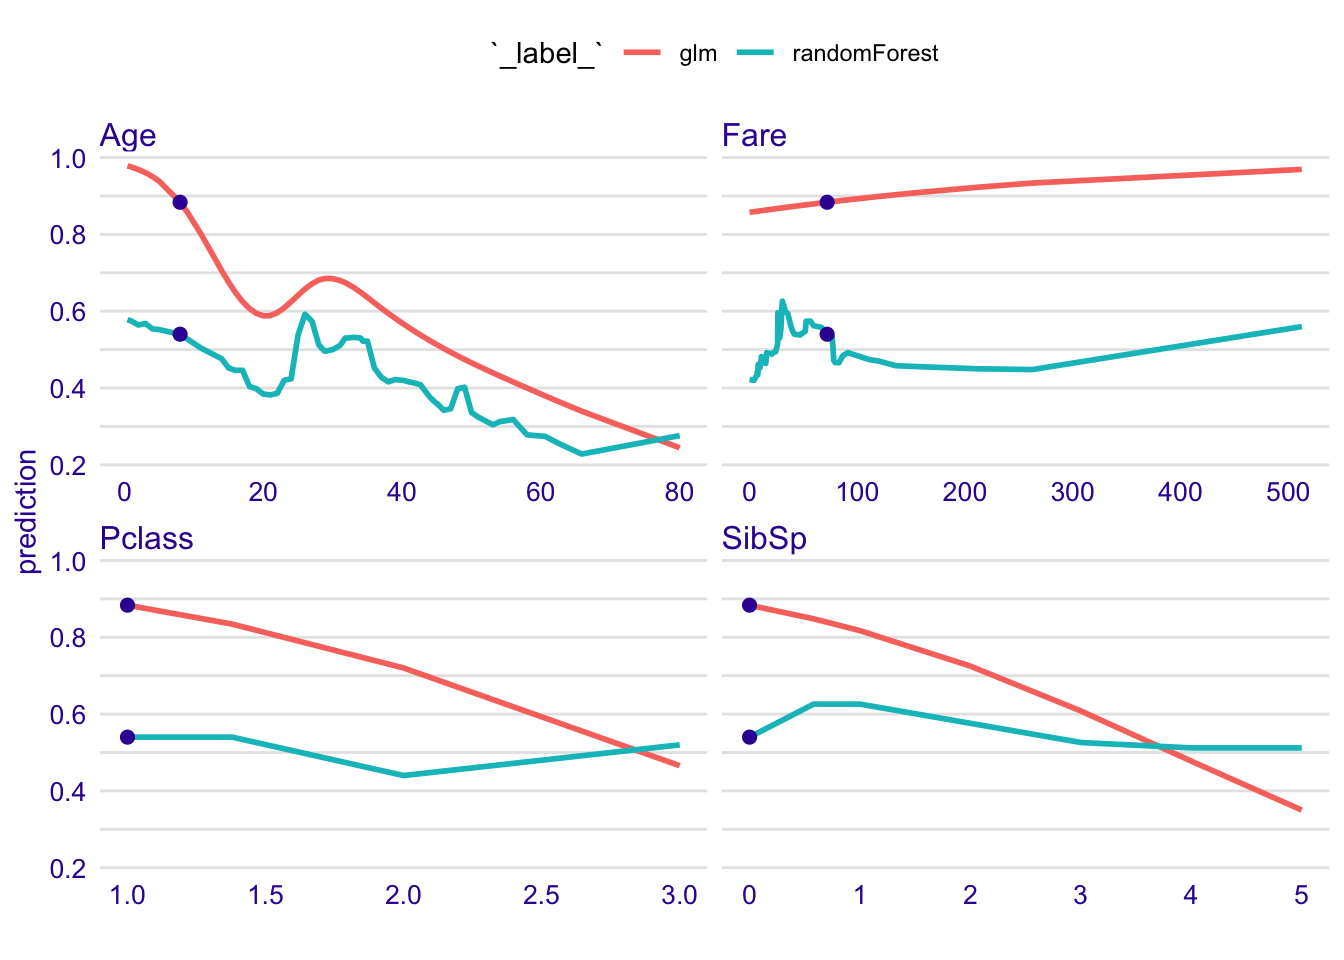
\includegraphics{PM_VEE_files/figure-latex/unnamed-chunk-25-1.pdf}

For selected profiles we can calculate oscillations with the
\texttt{calculate\_oscillations} function.

\begin{Shaded}
\begin{Highlighting}[]
\NormalTok{cpo_titanic_rf <-}\StringTok{ }\KeywordTok{calculate_oscillations}\NormalTok{(cp_titanic_rf)}
\NormalTok{cp_titanic_rf}\OperatorTok{$}\StringTok{`}\DataTypeTok{_ids_}\StringTok{`}\NormalTok{ =}\StringTok{ "Johny D"}
\NormalTok{cpo_titanic_rf}
\end{Highlighting}
\end{Shaded}

\begin{verbatim}
##   _vname_ _ids_ oscillations
## 1     age     1   0.21530192
## 4   parch     1   0.17182595
## 2    fare     1   0.07820906
## 3   sibsp     1   0.03507079
\end{verbatim}

The \texttt{calculate\_oscillations()} function returns an object of the
class \texttt{ceteris\_paribus\_oscillations}, which has a form of a
data frame but has also overloaded \texttt{plot()} function.

Use it to plot local variable importance for a selected observation

\begin{Shaded}
\begin{Highlighting}[]
\KeywordTok{plot}\NormalTok{(cpo_titanic_rf) }\OperatorTok{+}
\StringTok{  }\KeywordTok{ggtitle}\NormalTok{(}\StringTok{"Ceteris Paribus Oscillations"}\NormalTok{,}
          \StringTok{"For model_titanic_rf model"}\NormalTok{)}
\end{Highlighting}
\end{Shaded}

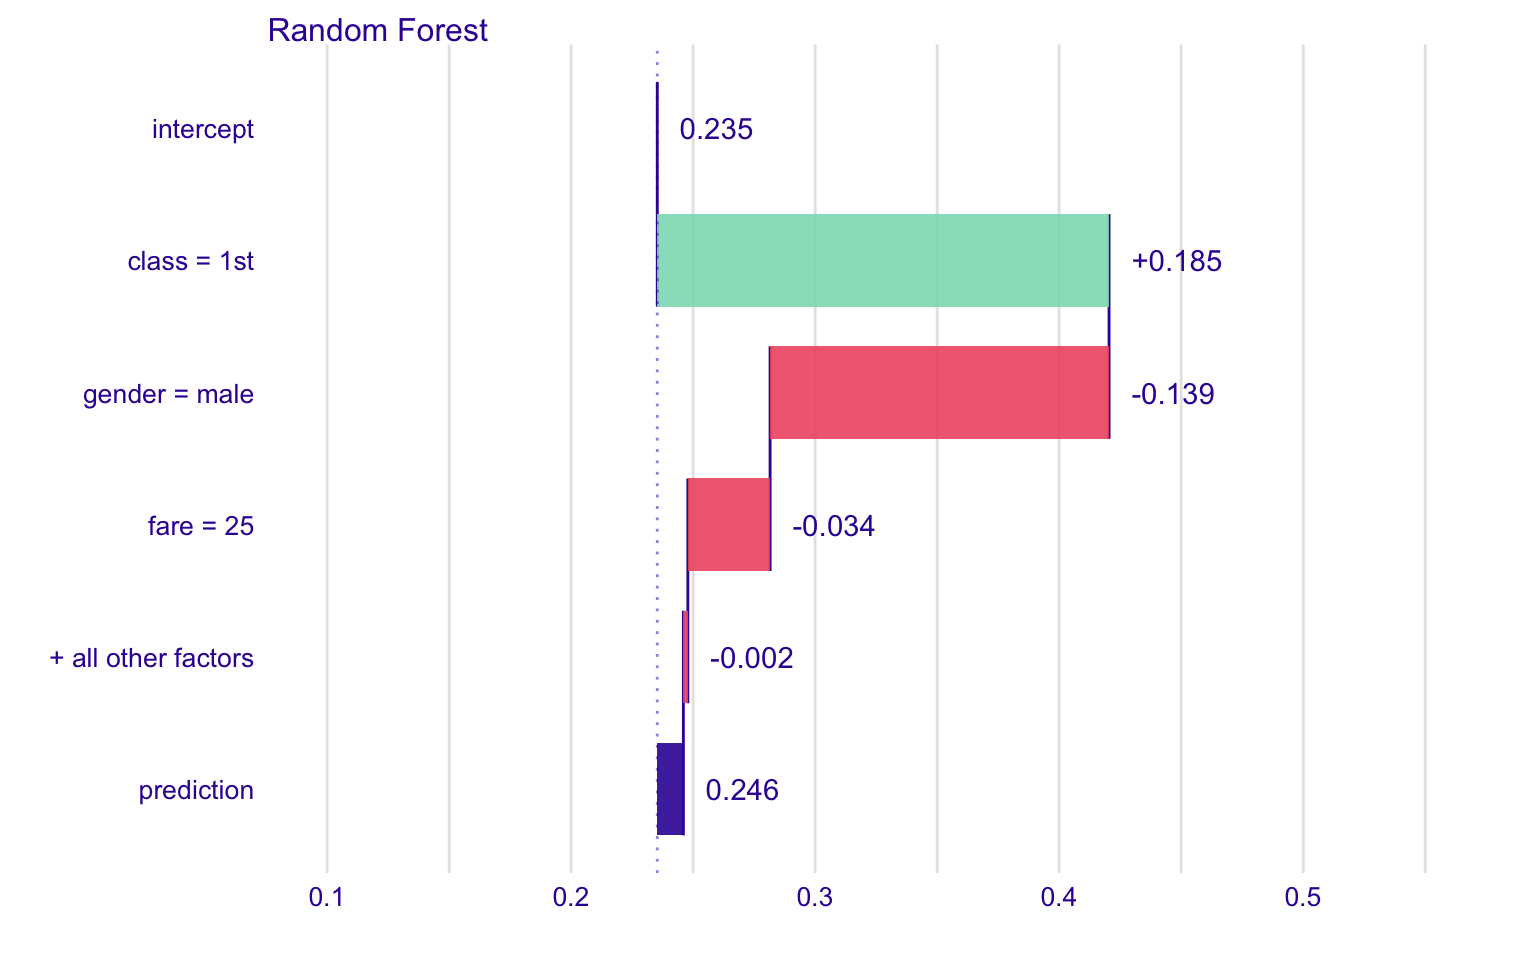
\includegraphics{PM_VEE_files/figure-latex/unnamed-chunk-27-1.pdf}

It looks like for Jony D. the two most important features are
\texttt{age} and \texttt{parch}. Higher \texttt{age} of this passenger
would significantly lower the chances of survival while higher
\texttt{parch} would increase these odds.

\hypertarget{ceterisParibus2d}{%
\section{Ceteris-Paribus 2D Profiles - a tool for pairwise
interactions}\label{ceterisParibus2d}}

\hypertarget{introduction-3}{%
\subsection{Introduction}\label{introduction-3}}

The definition of Ceteris Paribus profiles, given in Section
\ref{ceterisParibus}, may be easily extended to two or more explanatory
variables. Also, the definition of the variance importance measure
\(vip^{CP}_j(x^*)\) have a straightforward extension for a larger number
of variables.

Such extension is useful to identify or visualize of pairwise
interactions between variables.

\hypertarget{intuition-2}{%
\subsection{Intuition}\label{intuition-2}}

Figure \ref{fig:profile2d} presents a response surface for a
\texttt{titanic\_lmr\_v6} model for two explanatory variables,
\emph{age} and \emph{sibsp}, from the \emph{titanic} dataset (see
Section \ref{TitanicDataset}). We are interested in the change of the
model prediction induced by each of the variables.

\textbackslash{}begin\{figure\}

\{\centering 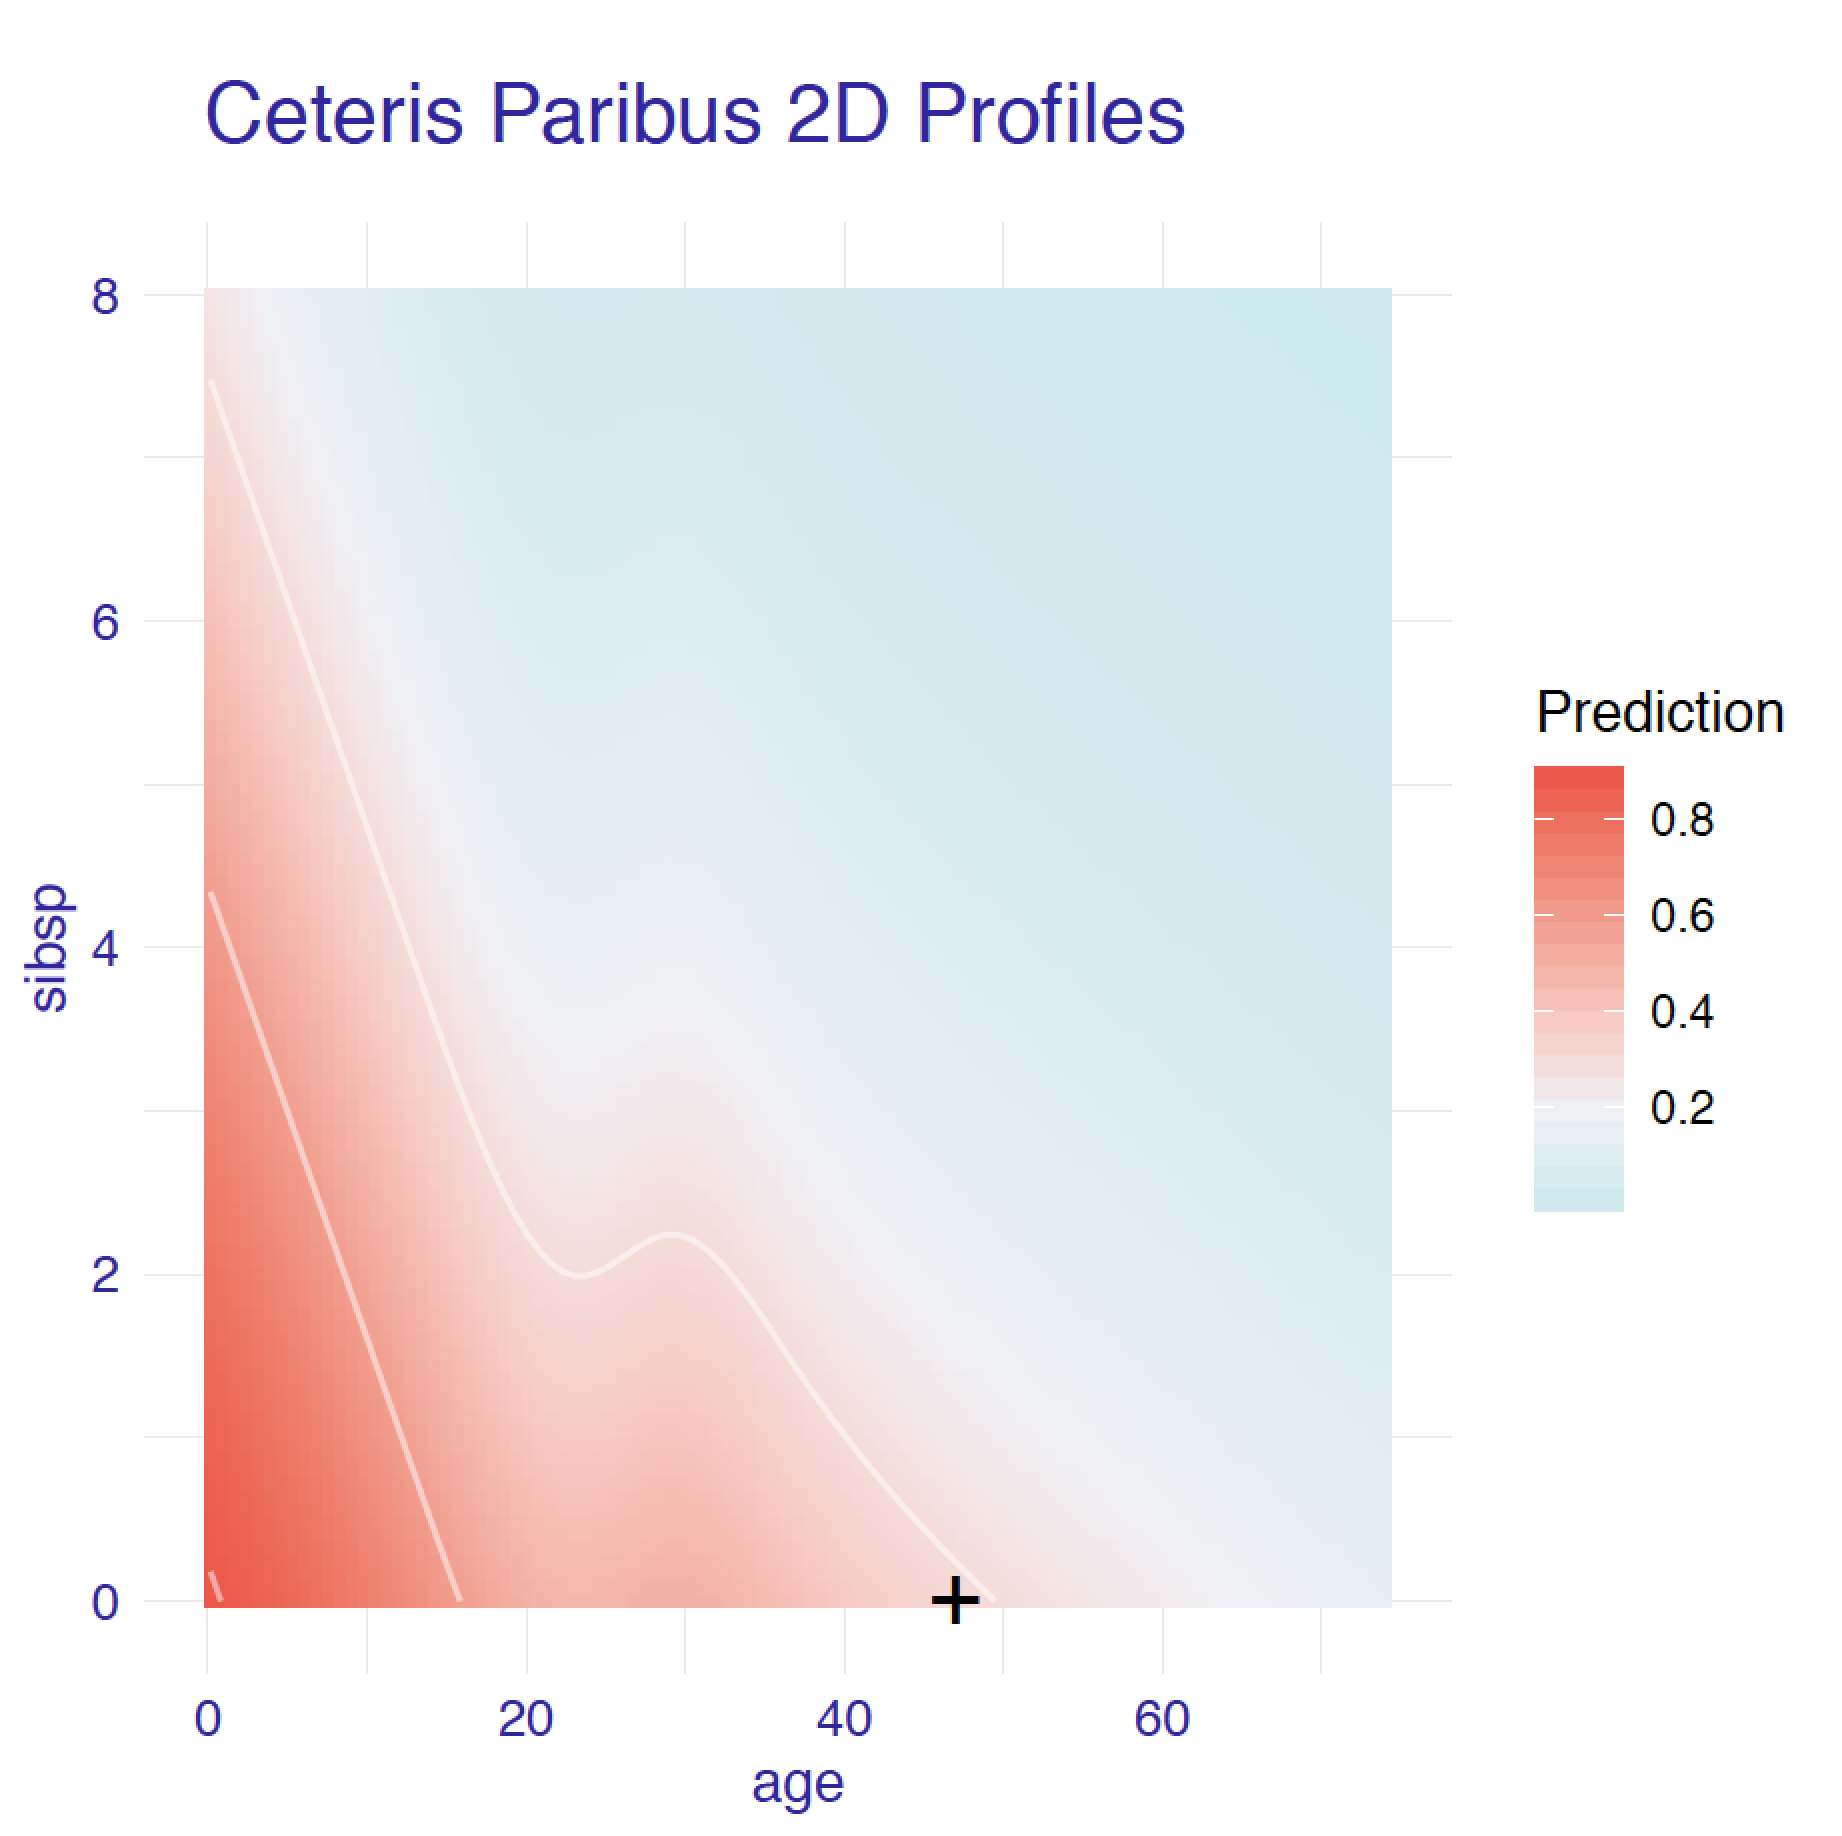
\includegraphics[width=0.7\linewidth]{figure/profile_2d}

\}

\textbackslash{}caption\{(fig:profile2d) Ceteris-paribus profile for a
pair of explanatory variables for a model \texttt{titanic\_lmer\_v6} for
\texttt{age} and \texttt{sibsp} variables.\}\label{fig:profile2d}
\textbackslash{}end\{figure\}

\hypertarget{method-2}{%
\subsection{Method}\label{method-2}}

The definition of Ceteris Paribus profiles may be easily extended to two
or more explanatory variables. A two-dimensional Ceteris Paribus profile
for model \(f\), explanatory variables \(j\) and \(k\), and point
\(x^*\) is defined as follows:

\[
CP^{f, (j,k), x^*}(z_1, z_2) \equiv f(x^*|^{(j,k)} = (z_1,z_2)).
\]

Ceteris Paribus 2D profile is a function that provides the dependence of
the prediction of the model on the values of \(j\)-th and \(k\)-th
explanatory variables \(z_1\) and \(z_2\), respectively, where \(z_1\)
and \(z_2\) are taken to go through the range of values typical for the
variables, and values of all other variables in \(x^*\) are kept fixed
at the values present in \(x^*\).

The corresponding variance importance measure would be defined as
follows: \[
vip^{CP}_{j,k}(x^*) = \int_{\mathcal R}\int_{\mathcal R} |CP^{f,(j,k),x^*}(z_1,z_2) - f(x^*)| g^{j,k}(z_1,z_2)dz_1dz_2=E_{X_j,X_k}[|CP^{f,j,x^*}(X_j,X_k) - f(x^*)|],
\] where the expected value is taken over the joint distribution of the
\(j\)-th and \(k\)-th explanatory variable.

Such multi-dimensional extensions are useful to check if, for instance,
the model involves interactions. In particular, presence of pairwise
interactions may be detected with two-dimensional (2D) CP profiles.

A natural way to visualize 2D CP profiles is to use a heat map for all
pairs of explanatory variables as in Figure \ref{fig:profile2dAll}.

\textbackslash{}begin\{figure\}

\{\centering 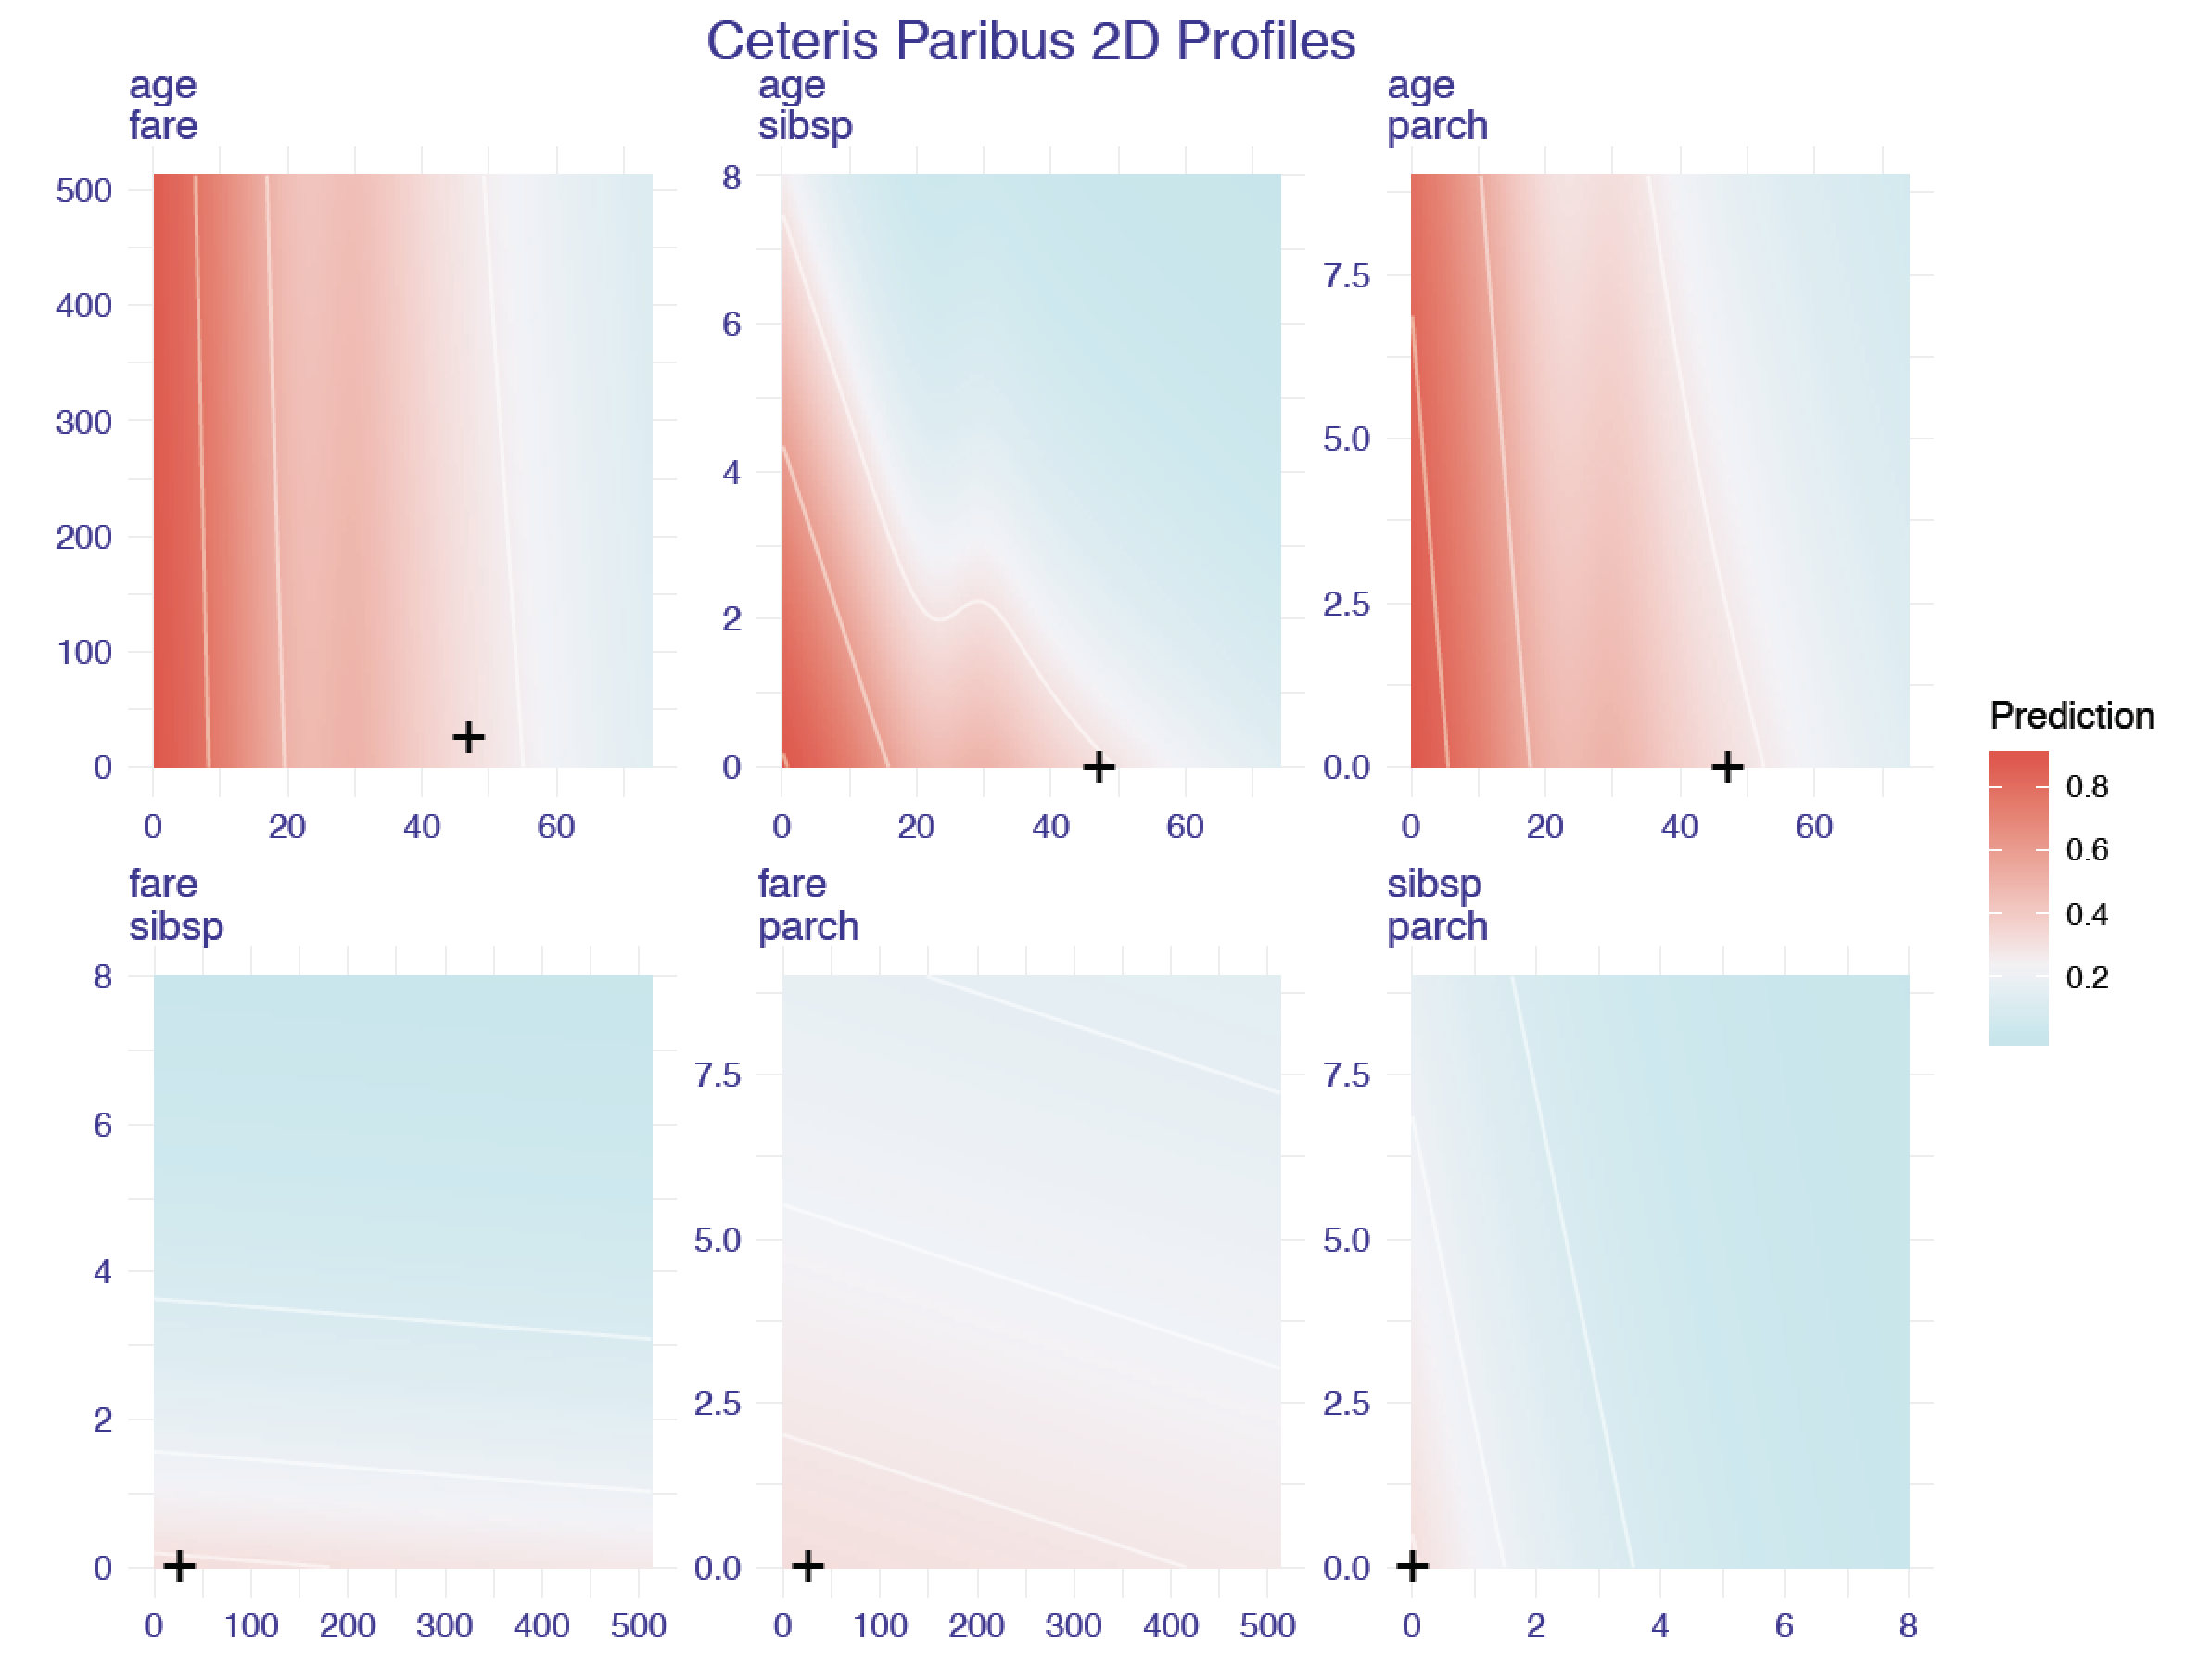
\includegraphics[width=0.9\linewidth]{figure/profile_2d_all}

\}

\textbackslash{}caption\{(fig:profile2dAll) Ceteris-paribus profile for
all pairs of explanatory variables for a \texttt{titanic\_lmer\_v6}
model. Black cross marks the coordinates of the point of
interest.\}\label{fig:profile2dAll} \textbackslash{}end\{figure\}

If the number of pairs of explanatory variables is small or moderate,
then it is possible to present 2D CP profiles for all pairs of
variables.

If the number of pairs is large, we can use the variable importance
measure to order the pairs based on their importance and select the most
important pairs for purposes of illustration.

\hypertarget{pros-and-cons-2}{%
\subsection{Pros and cons}\label{pros-and-cons-2}}

Two-dimensional CP profiles can be used to identify the presence of
pairwise interactions in a model.

But number of pairs may be large and 3d profiles are more difficult to
read than 1d profiles.

\hypertarget{code-snippets-for-r-2}{%
\subsection{Code snippets for R}\label{code-snippets-for-r-2}}

In this section we present key features of the R package
\texttt{ingredients} \citep{ingredientsRPackage} which is a part of
\texttt{DALEXverse} and covers all methods presented in this chapter.
More details and examples can be found at
\texttt{https://modeloriented.github.io/ingredients/}.

There are also other R packages that offer similar functionality, like
\texttt{condvis} \citep{JSSv081i05} or \texttt{ICEbox}
\citep{ICEboxRPackage}.

In this section we use a random forest \citep{R-randomForest} model
\texttt{titanic\_rf\_v6} developed for the Titanic dataset (see Section
\ref{TitanicDataset}). In particular, we deal with a binary
classification problem - we want to predict the probability of survival
for a selected passenger.

\begin{Shaded}
\begin{Highlighting}[]
\KeywordTok{library}\NormalTok{(}\StringTok{"DALEX"}\NormalTok{)}
\KeywordTok{library}\NormalTok{(}\StringTok{"randomForest"}\NormalTok{)}
\NormalTok{titanic <-}\StringTok{ }\KeywordTok{na.omit}\NormalTok{(titanic)}

\NormalTok{model_titanic_rf <-}\StringTok{ }\KeywordTok{randomForest}\NormalTok{(survived }\OperatorTok{==}\StringTok{ "yes"} \OperatorTok{~}\StringTok{ }\NormalTok{gender }\OperatorTok{+}\StringTok{ }\NormalTok{age }\OperatorTok{+}\StringTok{ }\NormalTok{class }\OperatorTok{+}\StringTok{ }\NormalTok{embarked }\OperatorTok{+}
\StringTok{                                   }\NormalTok{fare }\OperatorTok{+}\StringTok{ }\NormalTok{sibsp }\OperatorTok{+}\StringTok{ }\NormalTok{parch,  }\DataTypeTok{data =}\NormalTok{ titanic)}
\NormalTok{explain_titanic_rf <-}\StringTok{ }\KeywordTok{explain}\NormalTok{(}\DataTypeTok{model =}\NormalTok{ model_titanic_rf, }
                              \DataTypeTok{data =}\NormalTok{ titanic[,}\OperatorTok{-}\DecValTok{9}\NormalTok{],}
                              \DataTypeTok{y =}\NormalTok{ titanic}\OperatorTok{$}\NormalTok{survived }\OperatorTok{==}\StringTok{ "yes"}\NormalTok{, }
                              \DataTypeTok{label =} \StringTok{"Random Forest v7"}\NormalTok{)}
\end{Highlighting}
\end{Shaded}

In order to calculate oscillations we need to first calculate Ceteris
Paribus profiles for a selected observation.

Let us use the \texttt{johny\_d} instance again.

\begin{Shaded}
\begin{Highlighting}[]
\NormalTok{johny_d <-}\StringTok{ }\KeywordTok{data.frame}\NormalTok{(}
  \DataTypeTok{class =} \KeywordTok{factor}\NormalTok{(}\StringTok{"1st"}\NormalTok{, }\DataTypeTok{levels =} \KeywordTok{c}\NormalTok{(}\StringTok{"1st"}\NormalTok{, }\StringTok{"2nd"}\NormalTok{, }\StringTok{"3rd"}\NormalTok{, }\StringTok{"deck crew"}\NormalTok{, }\StringTok{"engineering crew"}\NormalTok{, }
                                  \StringTok{"restaurant staff"}\NormalTok{, }\StringTok{"victualling crew"}\NormalTok{)),}
  \DataTypeTok{gender =} \KeywordTok{factor}\NormalTok{(}\StringTok{"male"}\NormalTok{, }\DataTypeTok{levels =} \KeywordTok{c}\NormalTok{(}\StringTok{"female"}\NormalTok{, }\StringTok{"male"}\NormalTok{)),}
  \DataTypeTok{age =} \DecValTok{8}\NormalTok{,}
  \DataTypeTok{sibsp =} \DecValTok{0}\NormalTok{,}
  \DataTypeTok{parch =} \DecValTok{0}\NormalTok{,}
  \DataTypeTok{fare =} \DecValTok{72}\NormalTok{,}
  \DataTypeTok{embarked =} \KeywordTok{factor}\NormalTok{(}\StringTok{"Southampton"}\NormalTok{, }\DataTypeTok{levels =} \KeywordTok{c}\NormalTok{(}\StringTok{"Belfast"}\NormalTok{, }\StringTok{"Cherbourg"}\NormalTok{, }\StringTok{"Queenstown"}\NormalTok{, }\StringTok{"Southampton"}\NormalTok{))}
\NormalTok{)}
\end{Highlighting}
\end{Shaded}

2D profiles are calculated with the \texttt{ceteris\_paribus\_2d()}
function. By default all pairs between continuous variables are being
plotted, but one can limit number of variables for consideration through
the \texttt{variables} argument.

\begin{Shaded}
\begin{Highlighting}[]
\KeywordTok{library}\NormalTok{(}\StringTok{"ingredients"}\NormalTok{)}
\KeywordTok{library}\NormalTok{(}\StringTok{"ggplot2"}\NormalTok{)}

\NormalTok{wi_rf_2d <-}\StringTok{ }\KeywordTok{ceteris_paribus_2d}\NormalTok{(explain_titanic_rf, }\DataTypeTok{observation =}\NormalTok{ titanic[}\DecValTok{31}\NormalTok{,], }\DataTypeTok{variables =} \KeywordTok{c}\NormalTok{(}\StringTok{"age"}\NormalTok{, }\StringTok{"sibsp"}\NormalTok{, }\StringTok{"parch"}\NormalTok{))}
\KeywordTok{head}\NormalTok{(wi_rf_2d)}
\end{Highlighting}
\end{Shaded}

\begin{verbatim}
##        y_hat    new_x1 new_x2 vname1 vname2            label
## 31   0.61491 0.1666667   0.00    age  sibsp Random Forest v7
## 31.1 0.61491 0.1666667   0.08    age  sibsp Random Forest v7
## 31.2 0.61491 0.1666667   0.16    age  sibsp Random Forest v7
## 31.3 0.61491 0.1666667   0.24    age  sibsp Random Forest v7
## 31.4 0.61491 0.1666667   0.32    age  sibsp Random Forest v7
## 31.5 0.61491 0.1666667   0.40    age  sibsp Random Forest v7
\end{verbatim}

Result is an object of the class
\texttt{ceteris\_paribus\_2d\_explainer} with overloaded
\texttt{print()} and \texttt{plot()} function.

\begin{Shaded}
\begin{Highlighting}[]
\KeywordTok{plot}\NormalTok{(wi_rf_2d) }\OperatorTok{+}\StringTok{ }
\StringTok{  }\KeywordTok{theme}\NormalTok{(}\DataTypeTok{legend.position =} \StringTok{"right"}\NormalTok{, }\DataTypeTok{legend.direction =} \StringTok{"vertical"}\NormalTok{) }\OperatorTok{+}\StringTok{ }\KeywordTok{ggtitle}\NormalTok{(}\StringTok{"Ceteris Paribus 2D Profiles"}\NormalTok{)}
\end{Highlighting}
\end{Shaded}

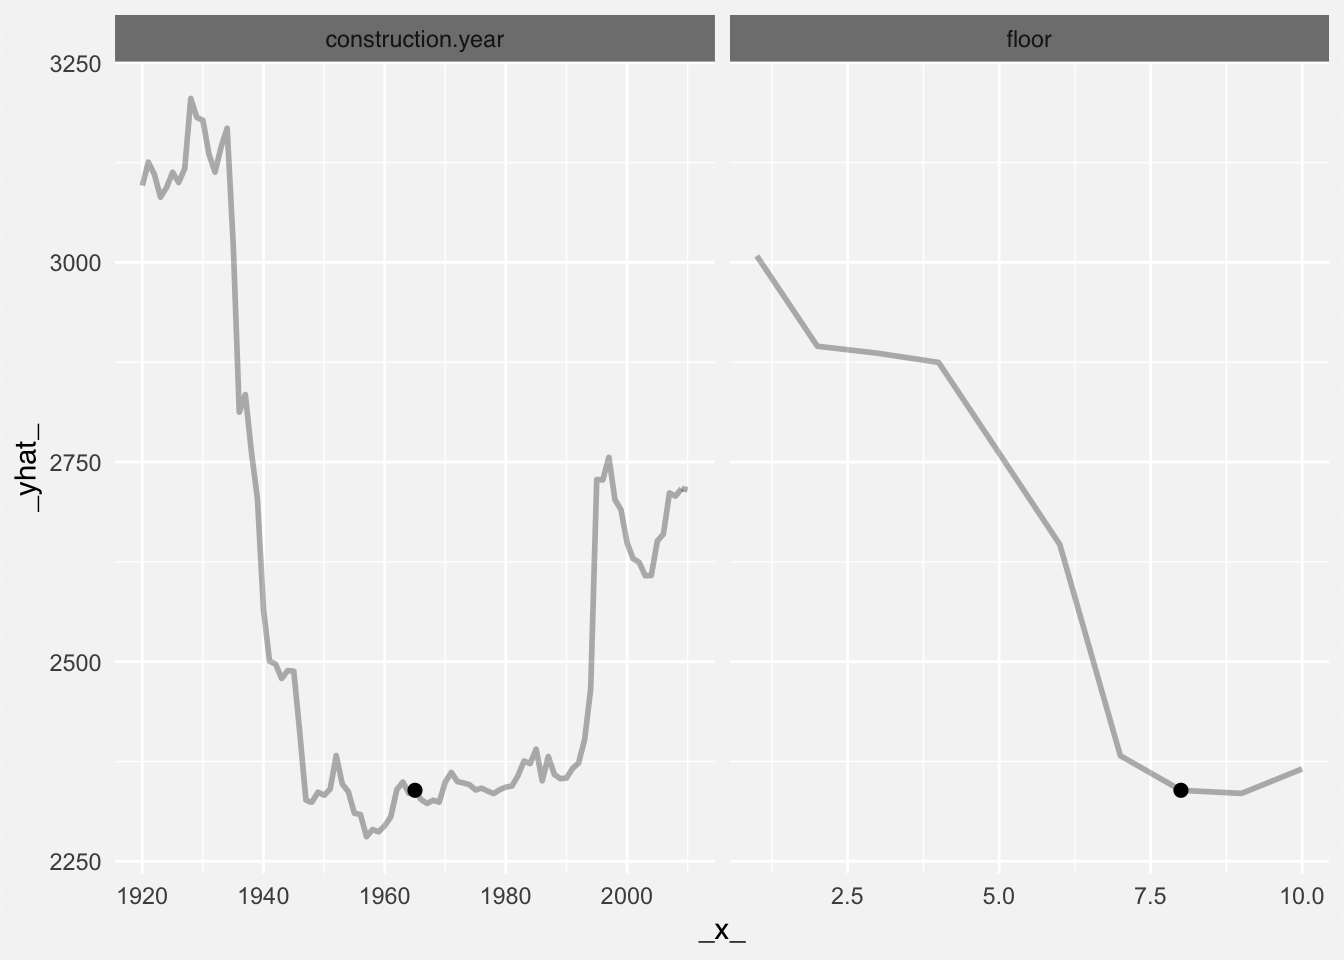
\includegraphics{PM_VEE_files/figure-latex/unnamed-chunk-31-1.pdf}

In the presented example both variables \texttt{age} and \texttt{sibsp}
are important and influence the model response.

\hypertarget{ceterisParibusWankardu}{%
\section{Local diagnostic with Ceteris-Paribus
profiles}\label{ceterisParibusWankardu}}

\hypertarget{introduction-4}{%
\subsection{Introduction}\label{introduction-4}}

What do you think, is it possible that model is good on average but
terrible for some observations?

I think that most of us would agree. But how we can check if a single
prediction is ,,unlucky''? In this chapter we present two techniques for
local model diagnostic that are based on Ceteris Paribus Profiles.

It may happen that global performance of the model is good, while for
some particular observations the fit is very bad. Local fidelity helps
to understand how good is the model fit at a particular observation. In
this section we show how to use Ceteris Paribus profiles to validate
local model fidelity.

The idea behind fidelity plots is to select a number of observatons
(``neighbors'') from the validation dataset that are closest to the
observation of interest. Then for the selected observations we plot CP
profiles and check how stable they are. Additionally, if we know true
values of the dependent variable for the selected neighbours, we may add
residuals to the plot to evaluate the local fit of the model.

\hypertarget{intuition-3}{%
\subsection{Intuition}\label{intuition-3}}

We want to diagnose model behavior around a single instance prediction.

One approach to local model validation is to examine how model behaves
for points from training data. See for example profiles presented in
Figure \ref{fig:profileWith10NN}. Ceteris Paribus Profiles are almost
parallel and close to each other what suggests that model is stable
around the point of interest.

It looks like small changes in the model input (represented by nearest
neighbors) do not influence model response in an unpredicted way.

\textbackslash{}begin\{figure\}

\{\centering 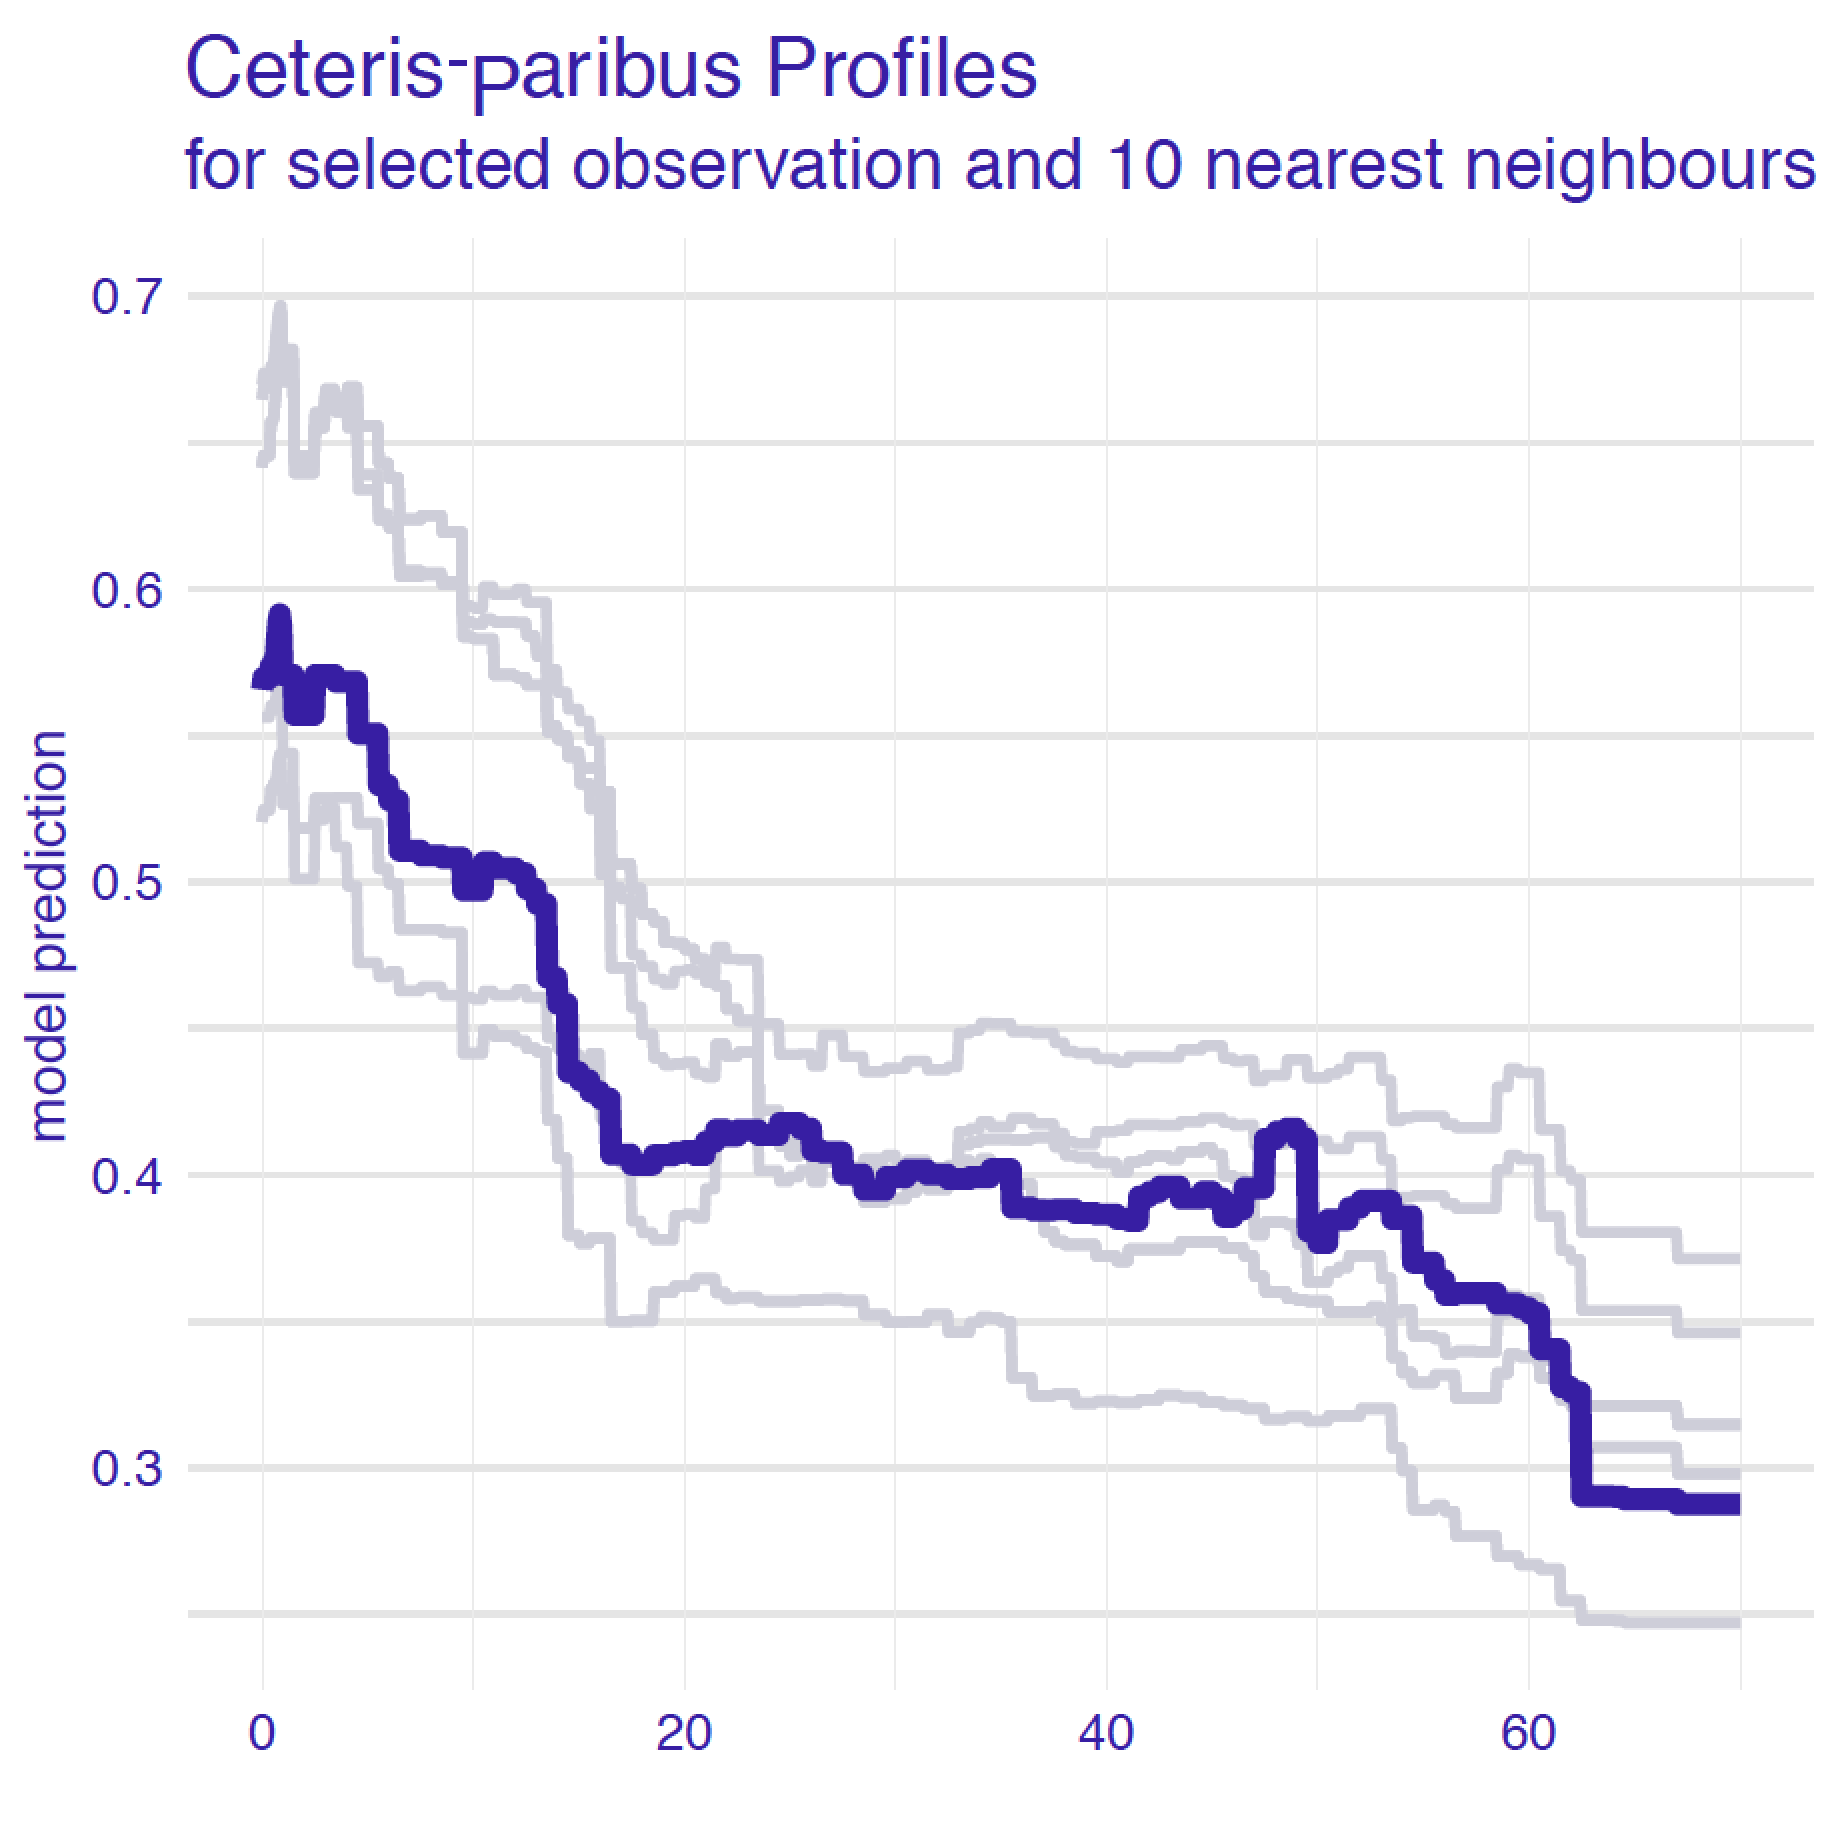
\includegraphics[width=0.5\linewidth]{figure/example_cp}

\}

\textbackslash{}caption\{(fig:profileWith10NN) Ceteris-paribus profiles
for a selected instance (dark violet line) and 10 nearest neighbors
(light grey lines). Note that these profiles are almost parallel and
close to each other what suggests the stability of the model. This
example is based on the \texttt{titanic\_rf\_b6} model and the
\texttt{titanic} dataset\}\label{fig:profileWith10NN}
\textbackslash{}end\{figure\}

Once we consider nearest neighbors we can also look closer on the model
fit around a specific point of interest. See for example the Figure
\ref{fig:profileBack2BackHist}. The back-to-back histogram shows
distribution of residuals for the whole validation data and selected
neighbors.

Distribution of residuals for the whole validation dataset is rather
symmetric and centered around 0. Residuals for neighbors are centered on
500, what means that the average model bias around the point of interest
is close to 500.

In the figure we showed an example in which residuals for nearest
neighbors are larger than average residuals. Thus the local model fit is
smaller than the global model fit.

\textbackslash{}begin\{figure\}

\{\centering 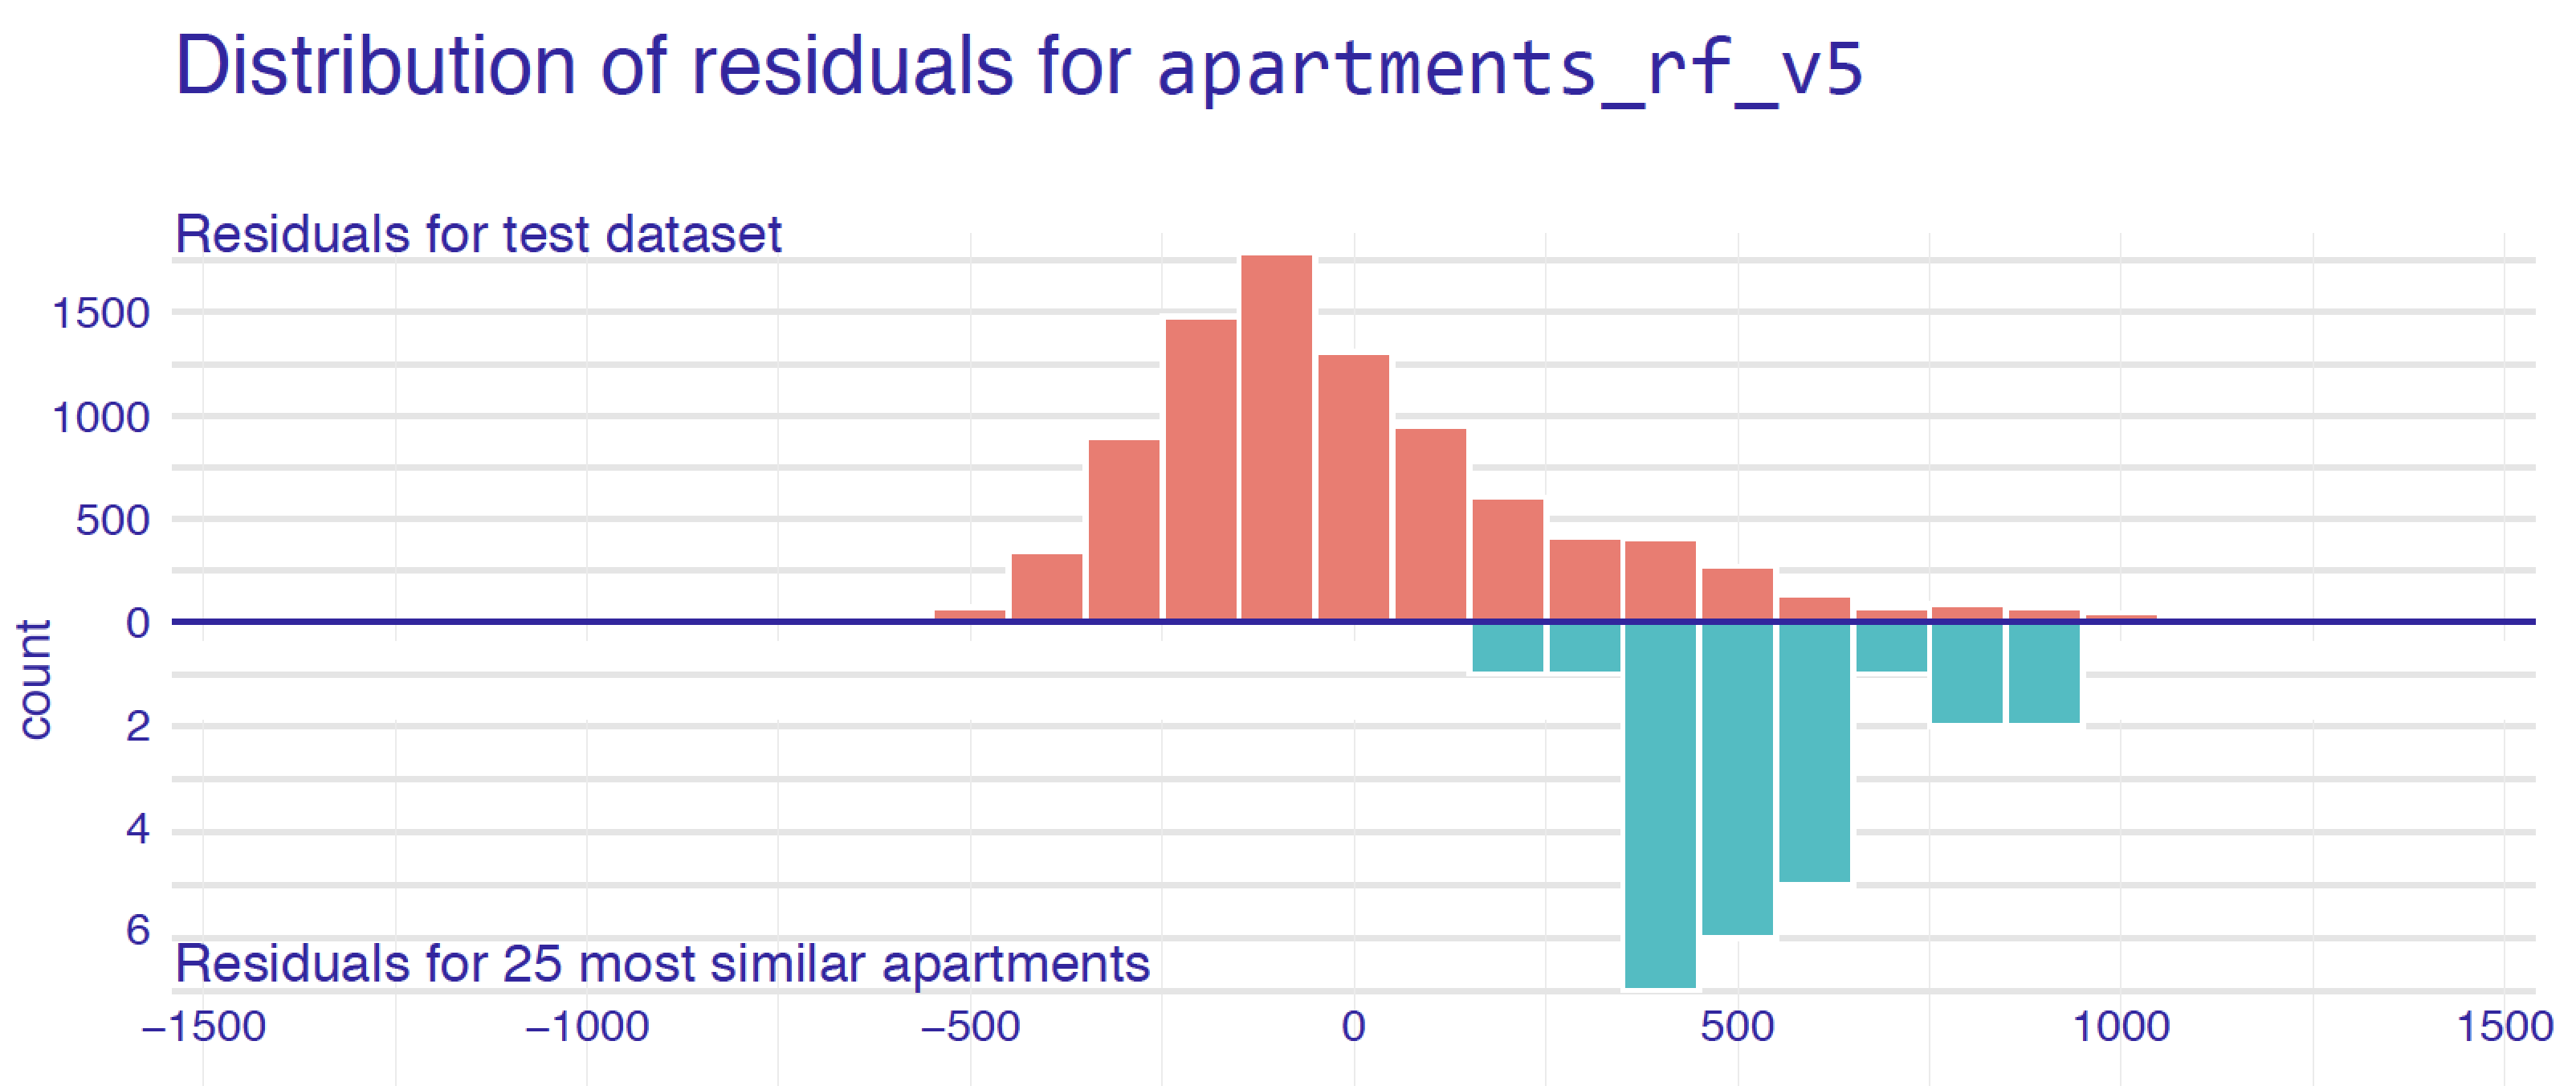
\includegraphics[width=0.7\linewidth]{figure/bb_hist}

\}

\textbackslash{}caption\{(fig:profileBack2BackHist) Back-to-back
histograms for residuals calculated with the \texttt{apartments\_rf\_v5}
model on \texttt{apartments} data. Upper panel correspond to residuals
calculated for all observations in the validation dataset while the
bottom panel correspond to residuals calculated for nearest neighbors.
Their residuals are higher than average model
residuals.\}\label{fig:profileBack2BackHist} \textbackslash{}end\{figure\}

\hypertarget{method-3}{%
\subsection{Method}\label{method-3}}

Local diagnostic is based on three elements.

\begin{itemize}
\tightlist
\item
  identification of nearest neighbors,
\item
  calculation and visualization of Ceteris Paribus profiles for selected
  neighbors,
\item
  analysis of residuals for nearest neighbors.
\end{itemize}

Let us discuss them point by point.

\hypertarget{nearest-neighbors}{%
\subsubsection{Nearest neighbors}\label{nearest-neighbors}}

How many nearest neighbors shall we choose and what metric can we use?

Answer for both questions is of course \emph{it depends}.

\begin{itemize}
\tightlist
\item
  The smaller the number of neighbors is the more local is the analysis.
  But very small numbers lead to larger variability of the diagnosis.
  The default value in the \texttt{select\_neighbours()} function is
  \texttt{n\ =\ 20}.
\item
  The distance measure if very important. The higher the dimension the
  more crucial is this choice. For tabular data we additionally need to
  face a problem of different distributions of different features. The
  default choice in the \texttt{select\_neighbours()} function is to use
  \texttt{distance\ =\ gower\_dist()} function from the \texttt{gower}
  package \citep{gowerRPackage}. The Gower distance is an average from
  normalized distances \(d_k()\) calculated for particular features.
\end{itemize}

\[
d_{gower}(x^i, x^j) = \frac 1p \sum_{k=1}^p d_k(x_k^i, x_k^j).
\] * Distance can be calculated based on selected variables. In the
\texttt{select\_neighbours()} function one can specify them in the
\texttt{variables} argument.

\hypertarget{profiles-for-neighbors}{%
\subsubsection{Profiles for neighbors}\label{profiles-for-neighbors}}

Once nearest neighbors are identified we can compare Ceteris Paribus
profiles for selected variables.

If the number of features is large, then we can easily end up with bunch
of very similar small plots with spaghetti profiles. Better strategy
would be to focus only on profiles for the k-most important features. In
this chapter we show profiles only for a single variable. This makes
examples easier to read without reducing the generality.

For better readability we show only profiles for continuous variables.

\hypertarget{residuals}{%
\subsubsection{Residuals}\label{residuals}}

Ceteris Paribus profiles that assess model stability. In addition we can
add examination of the local residuals that assess local model fit.

Residuals for observation \(x^i\) are here defined as the difference
between the observed \(y^i\) and predicted \(x^i\), that is

\[
r^i = y^i - f(x^i).
\]

\hypertarget{local-fidelity-plot}{%
\subsubsection{Local Fidelity Plot}\label{local-fidelity-plot}}

Both residuals and Ceteris Paribus Profiles for nearest neighbors can be
presented in a single plot, called Local Fidelity Plot. See an example
in the Figure \ref{fig:localFidelityPlots}.

Such plots are complex as they convey lots of information. Yet it is not
that hard to learn how to read this information.

The Figure \ref{fig:localFidelityPlots} shows meaning of every element
of the plot. For a single instance, here the passenger Johnny D, we can
read how large are residuals for its neighbor, whatever residuals are
biased or symmetric, if Ceteris Profiles are stable and parallel.

\begin{figure}

{\centering 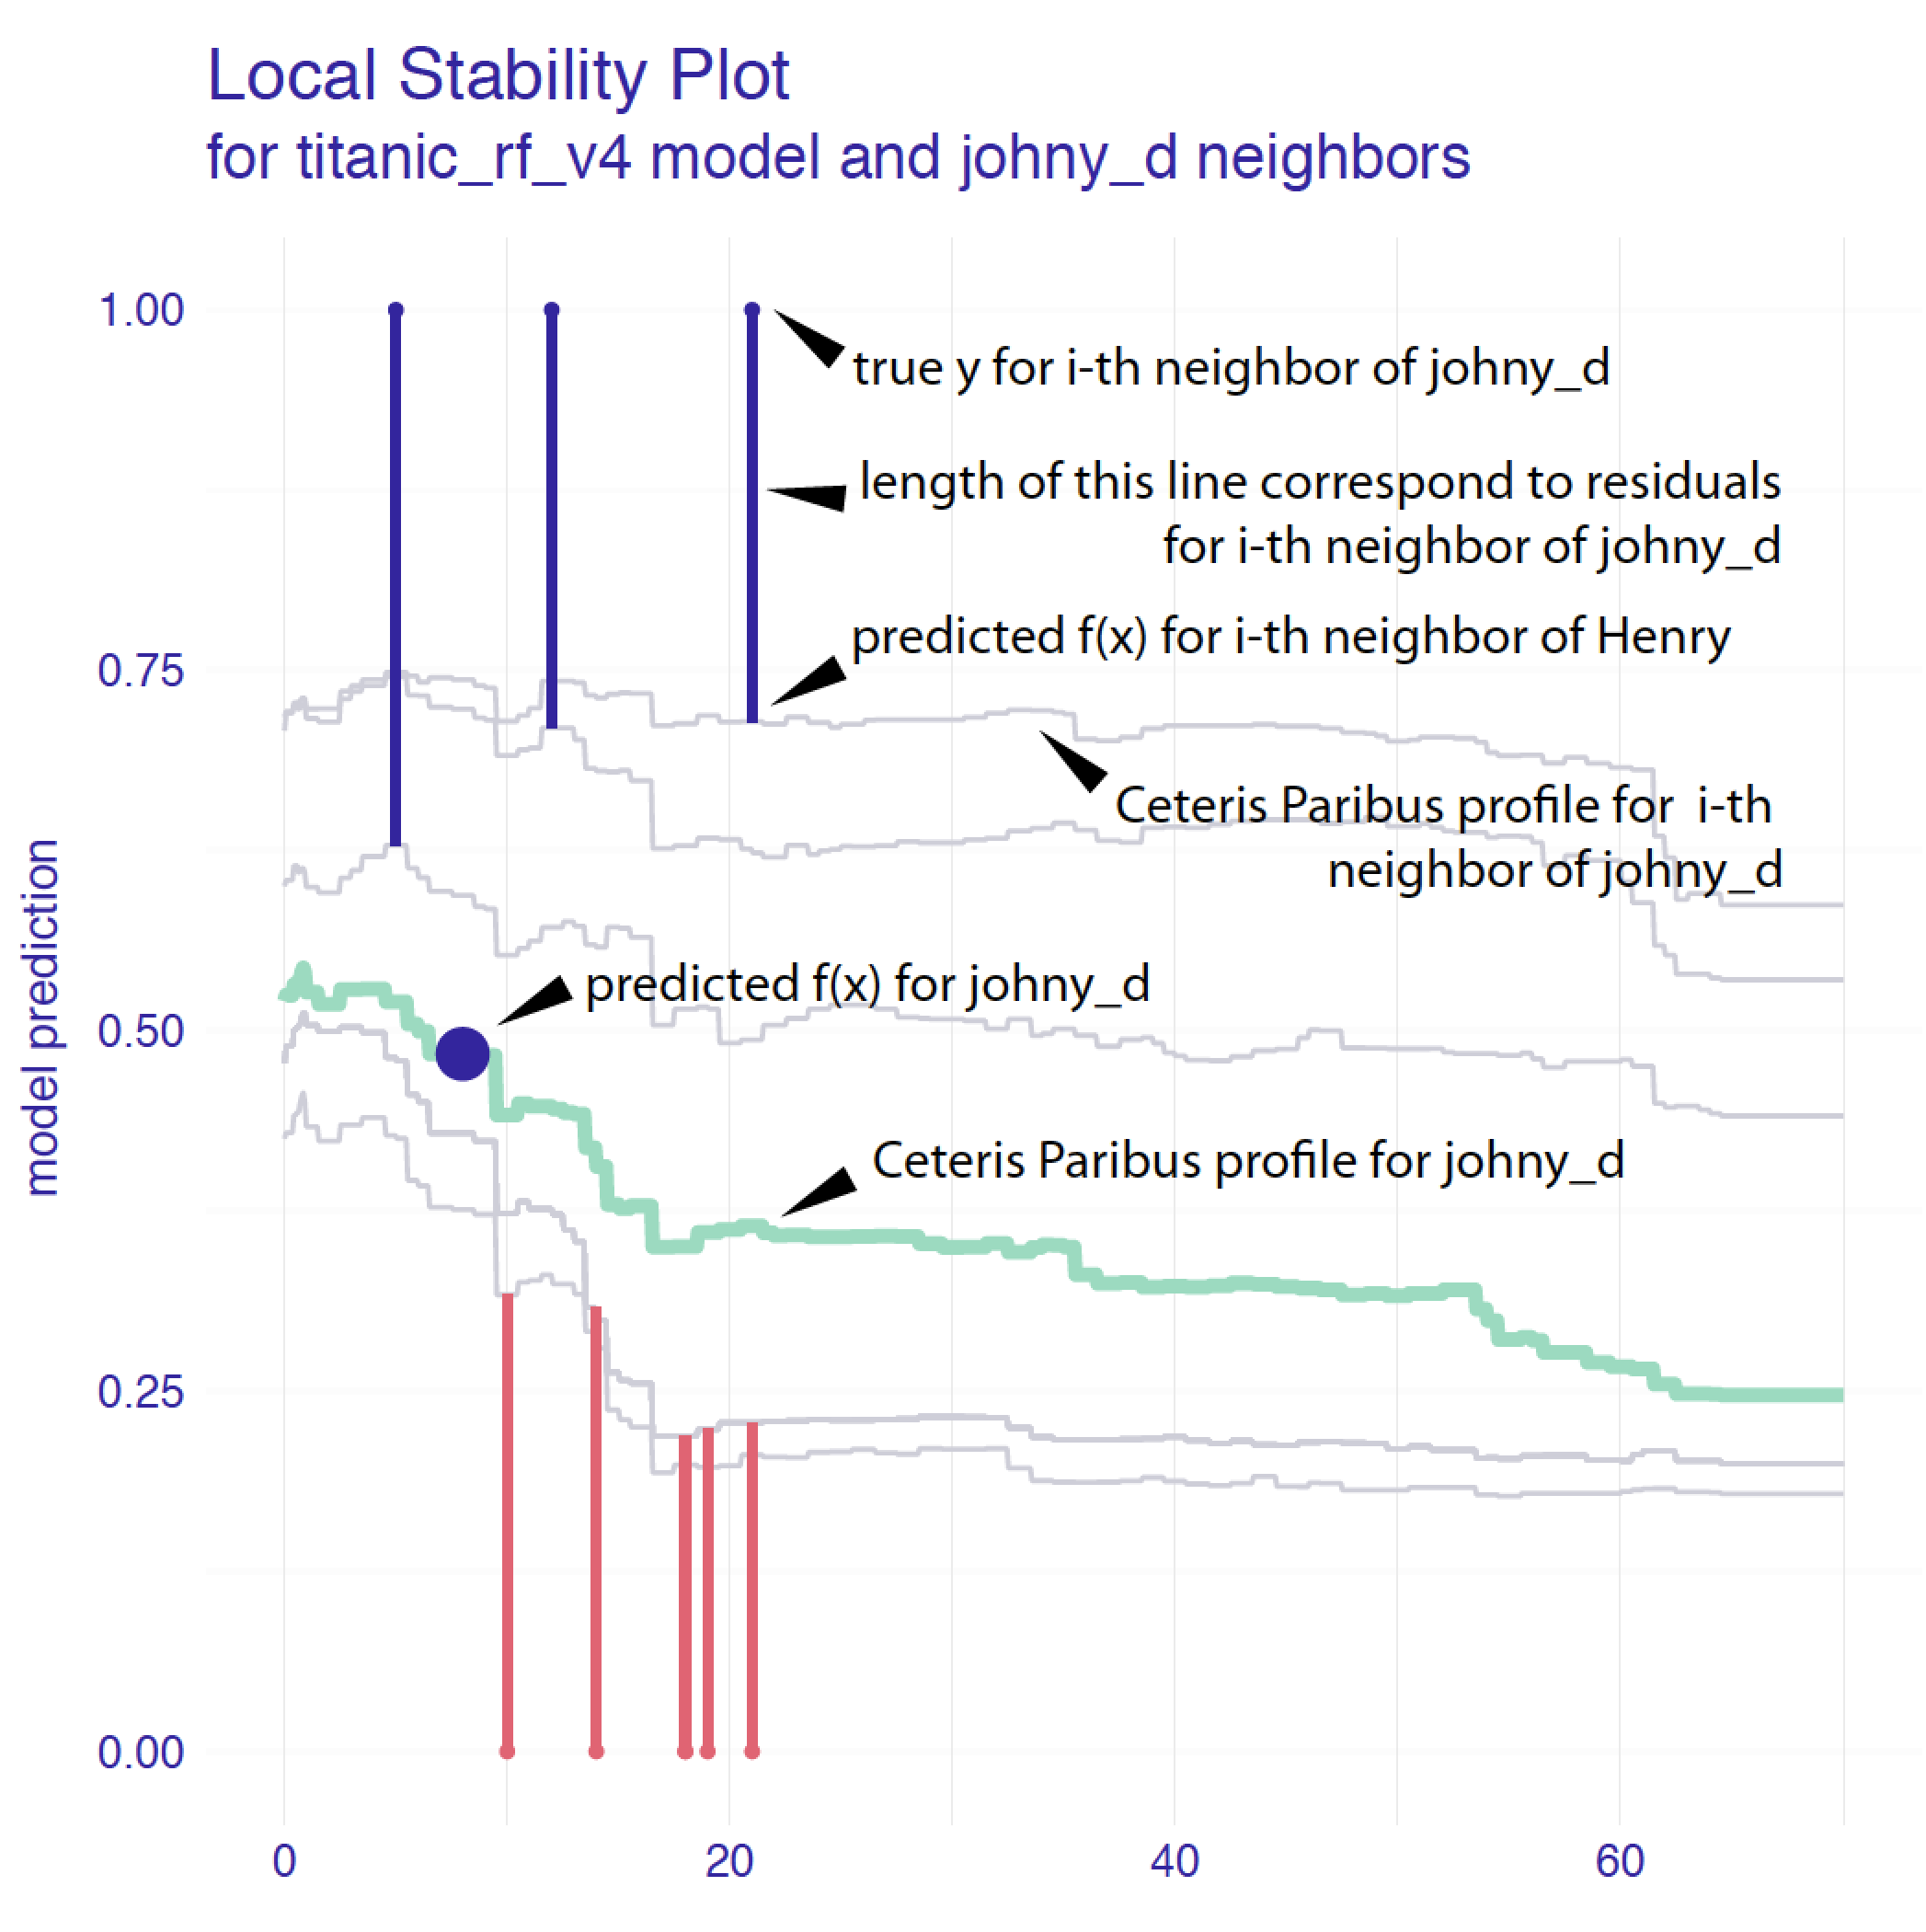
\includegraphics[width=0.7\linewidth]{figure/localFidelityPlots} 

}

\caption{(fig:localFidelityPlots) Elements of Local Fidelity Plots. Vertical intervals correspond to residuals, the smaller the more accurate is the model. Residuals are color coded, so we can easier recognized if they are biased or not, here there are balanced. Ceteris Paribus Profiles for neighbors are marked with grey lines. Stable model will have profiles close to each other; additive model will have parallel lines.}\label{fig:localFidelityPlots}
\end{figure}

\hypertarget{pros-and-cons-3}{%
\subsection{Pros and cons}\label{pros-and-cons-3}}

Local diagnostic plots may be very helpful to validate if

\begin{itemize}
\tightlist
\item
  model is additive locally (CP profiles are parallel),
\item
  model is stable locally (CP profiles are close to each other),
\item
  local fit is good (residuals are small and symmetric).
\end{itemize}

The drawback is that such plots are quite complex and lack objective
measures for quality of fit. As most diagnostic tools it's suited for
exploratory analysis.

\hypertarget{code-snippets-for-r-3}{%
\subsection{Code snippets for R}\label{code-snippets-for-r-3}}

In this section we show how to use an R package \texttt{ingredients}
\citep{R-ingredients} for the Local Fidelity Plots. More details and
examples can be found at
\texttt{https://modeloriented.github.io/ingredients/}.

In this section we use a random forest \citep{R-randomForest} model
\texttt{titanic\_rf\_v6} developed for the Titanic dataset (see Section
@ref\{model\_titanic\_rf\}). In particular, we deal with a binary
classification problem - we want to predict the probability of survival
for a selected passenger.

\begin{Shaded}
\begin{Highlighting}[]
\KeywordTok{library}\NormalTok{(}\StringTok{"DALEX"}\NormalTok{)}
\NormalTok{titanic <-}\StringTok{ }\KeywordTok{na.omit}\NormalTok{(titanic)}
\KeywordTok{library}\NormalTok{(}\StringTok{"randomForest"}\NormalTok{)}
\NormalTok{titanic_rf_v6 <-}\StringTok{ }\KeywordTok{randomForest}\NormalTok{(survived }\OperatorTok{==}\StringTok{ "yes"} \OperatorTok{~}\StringTok{ }\NormalTok{gender }\OperatorTok{+}\StringTok{ }\NormalTok{age }\OperatorTok{+}\StringTok{ }\NormalTok{class }\OperatorTok{+}\StringTok{ }\NormalTok{embarked }\OperatorTok{+}
\StringTok{                                   }\NormalTok{fare }\OperatorTok{+}\StringTok{ }\NormalTok{sibsp }\OperatorTok{+}\StringTok{ }\NormalTok{parch,  }\DataTypeTok{data =}\NormalTok{ titanic)}

\NormalTok{explain_titanic_rf <-}\StringTok{ }\KeywordTok{explain}\NormalTok{(}\DataTypeTok{model =}\NormalTok{ titanic_rf_v6, }
                              \DataTypeTok{data =}\NormalTok{ titanic[,}\OperatorTok{-}\DecValTok{9}\NormalTok{],}
                              \DataTypeTok{y =}\NormalTok{ titanic}\OperatorTok{$}\NormalTok{survived }\OperatorTok{==}\StringTok{ "yes"}\NormalTok{, }
                              \DataTypeTok{label =} \StringTok{"Random Forest v7"}\NormalTok{)}
\end{Highlighting}
\end{Shaded}

Local diagnostic is specified for an instance. Let us define a new
observation - 8 years old Johnny D, male passenger of the 1st class.

\begin{Shaded}
\begin{Highlighting}[]
\NormalTok{johny_d <-}\StringTok{ }\KeywordTok{data.frame}\NormalTok{(}
  \DataTypeTok{class =} \KeywordTok{factor}\NormalTok{(}\StringTok{"1st"}\NormalTok{, }\DataTypeTok{levels =} \KeywordTok{c}\NormalTok{(}\StringTok{"1st"}\NormalTok{, }\StringTok{"2nd"}\NormalTok{, }\StringTok{"3rd"}\NormalTok{, }\StringTok{"deck crew"}\NormalTok{, }\StringTok{"engineering crew"}\NormalTok{, }
                                  \StringTok{"restaurant staff"}\NormalTok{, }\StringTok{"victualling crew"}\NormalTok{)),}
  \DataTypeTok{gender =} \KeywordTok{factor}\NormalTok{(}\StringTok{"male"}\NormalTok{, }\DataTypeTok{levels =} \KeywordTok{c}\NormalTok{(}\StringTok{"female"}\NormalTok{, }\StringTok{"male"}\NormalTok{)),}
  \DataTypeTok{age =} \DecValTok{8}\NormalTok{,}
  \DataTypeTok{sibsp =} \DecValTok{0}\NormalTok{,}
  \DataTypeTok{parch =} \DecValTok{0}\NormalTok{,}
  \DataTypeTok{fare =} \DecValTok{72}\NormalTok{,}
  \DataTypeTok{embarked =} \KeywordTok{factor}\NormalTok{(}\StringTok{"Southampton"}\NormalTok{, }\DataTypeTok{levels =} \KeywordTok{c}\NormalTok{(}\StringTok{"Belfast"}\NormalTok{, }\StringTok{"Cherbourg"}\NormalTok{, }\StringTok{"Queenstown"}\NormalTok{, }\StringTok{"Southampton"}\NormalTok{))}
\NormalTok{)}
\end{Highlighting}
\end{Shaded}

\hypertarget{start-with-ceteris-paribus-profile}{%
\subsubsection{Start with Ceteris Paribus
Profile}\label{start-with-ceteris-paribus-profile}}

First we will plot a Ceteri Paribus Profiles for the observation of
interese.

\begin{Shaded}
\begin{Highlighting}[]
\KeywordTok{library}\NormalTok{(}\StringTok{"ingredients"}\NormalTok{)}
\KeywordTok{library}\NormalTok{(}\StringTok{"ggplot2"}\NormalTok{)}

\NormalTok{cp_johny <-}\StringTok{ }\KeywordTok{ceteris_paribus}\NormalTok{(explain_titanic_rf, johny_d, }\DataTypeTok{variable_splits =} \KeywordTok{list}\NormalTok{(}\DataTypeTok{age =} \DecValTok{0}\OperatorTok{:}\DecValTok{70}\NormalTok{))}
\KeywordTok{plot}\NormalTok{(cp_johny) }\OperatorTok{+}
\StringTok{  }\KeywordTok{show_observations}\NormalTok{(cp_johny, }\DataTypeTok{variables =} \StringTok{"age"}\NormalTok{) }\OperatorTok{+}
\StringTok{  }\KeywordTok{ggtitle}\NormalTok{(}\StringTok{"Ceteris Paribus Profile for Johnny D"}\NormalTok{,}\StringTok{"Calculated for titanic_rf_v6 model"}\NormalTok{)}
\end{Highlighting}
\end{Shaded}

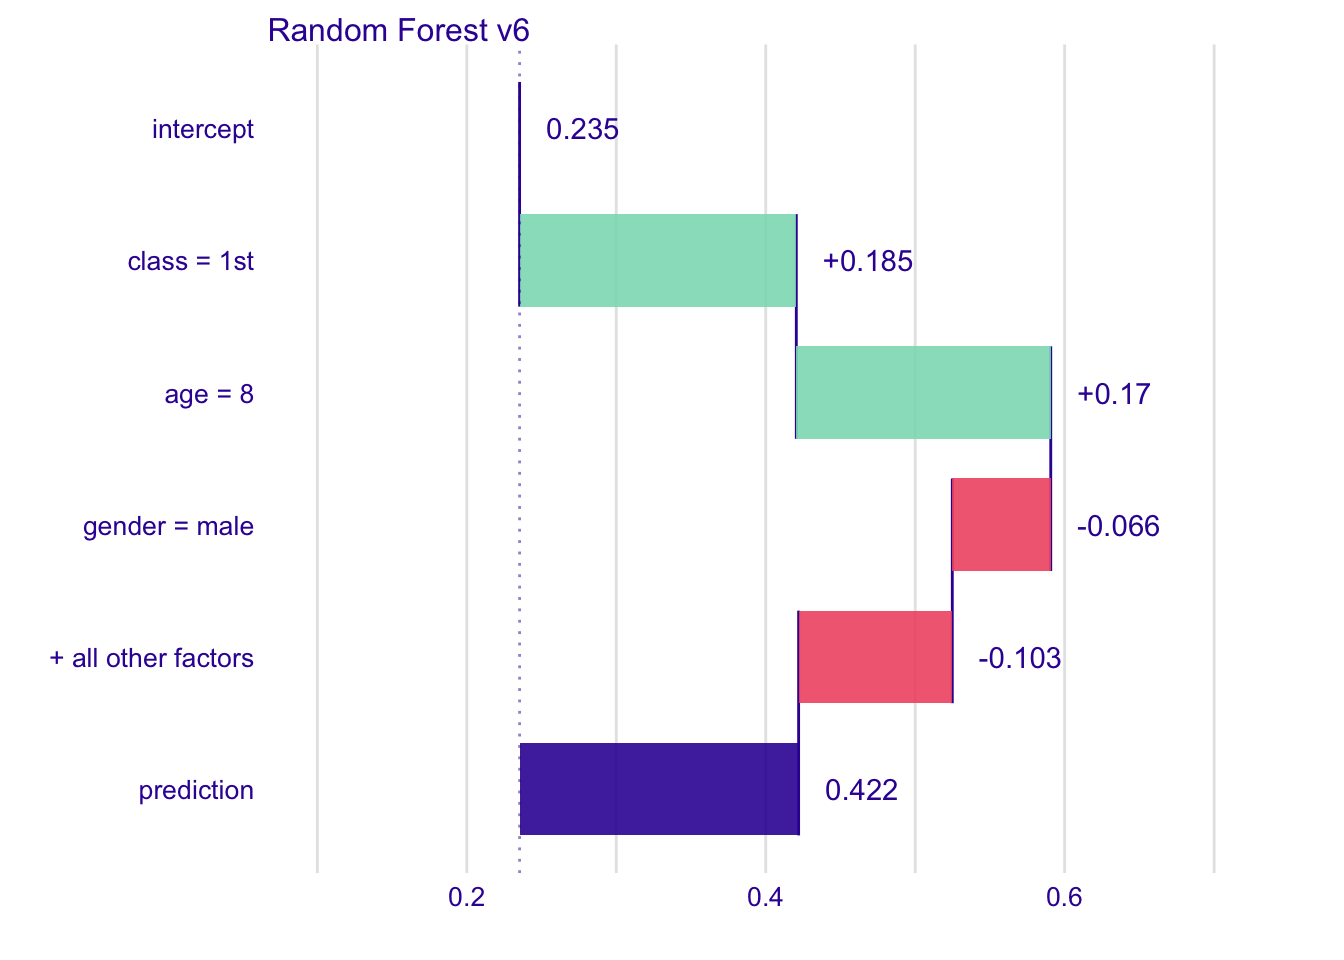
\includegraphics{PM_VEE_files/figure-latex/unnamed-chunk-34-1.pdf}

In the model chances of survival diminish with age. Johnny D is lucky to
have chances higher than 50\%.

\hypertarget{add-profiles-for-neighbors}{%
\subsubsection{Add profiles for
neighbors}\label{add-profiles-for-neighbors}}

Second we need to identify neighbors and plot their profiles.

\begin{Shaded}
\begin{Highlighting}[]
\NormalTok{johny_neighbors <-}\StringTok{ }\KeywordTok{select_neighbours}\NormalTok{(titanic, johny_d, }\DataTypeTok{n =} \DecValTok{10}\NormalTok{, }\DataTypeTok{variables =} \KeywordTok{c}\NormalTok{(}\StringTok{"age"}\NormalTok{, }\StringTok{"class"}\NormalTok{, }\StringTok{"gender"}\NormalTok{))}

\NormalTok{cp_johny_neighbors <-}\StringTok{ }\KeywordTok{ceteris_paribus}\NormalTok{(explain_titanic_rf, johny_neighbors, }
                                      \DataTypeTok{y =}\NormalTok{ johny_neighbors}\OperatorTok{$}\NormalTok{survived }\OperatorTok{==}\StringTok{ "yes"}\NormalTok{,}
                                      \DataTypeTok{variable_splits =} \KeywordTok{list}\NormalTok{(}\DataTypeTok{age =} \DecValTok{0}\OperatorTok{:}\DecValTok{70}\NormalTok{))}

\KeywordTok{plot}\NormalTok{(cp_johny) }\OperatorTok{+}
\StringTok{  }\KeywordTok{show_profiles}\NormalTok{(cp_johny_neighbors, }\DataTypeTok{color =} \StringTok{'#ceced9'}\NormalTok{) }\OperatorTok{+}\StringTok{ }
\StringTok{  }\KeywordTok{show_observations}\NormalTok{(cp_johny, }\DataTypeTok{variables =} \StringTok{"age"}\NormalTok{) }\OperatorTok{+}
\StringTok{  }\KeywordTok{ggtitle}\NormalTok{(}\StringTok{"Ceteris Paribus Profile for Johnny D and neighbors"}\NormalTok{,}\StringTok{"Calculated for titanic_rf_v6 model"}\NormalTok{)}
\end{Highlighting}
\end{Shaded}

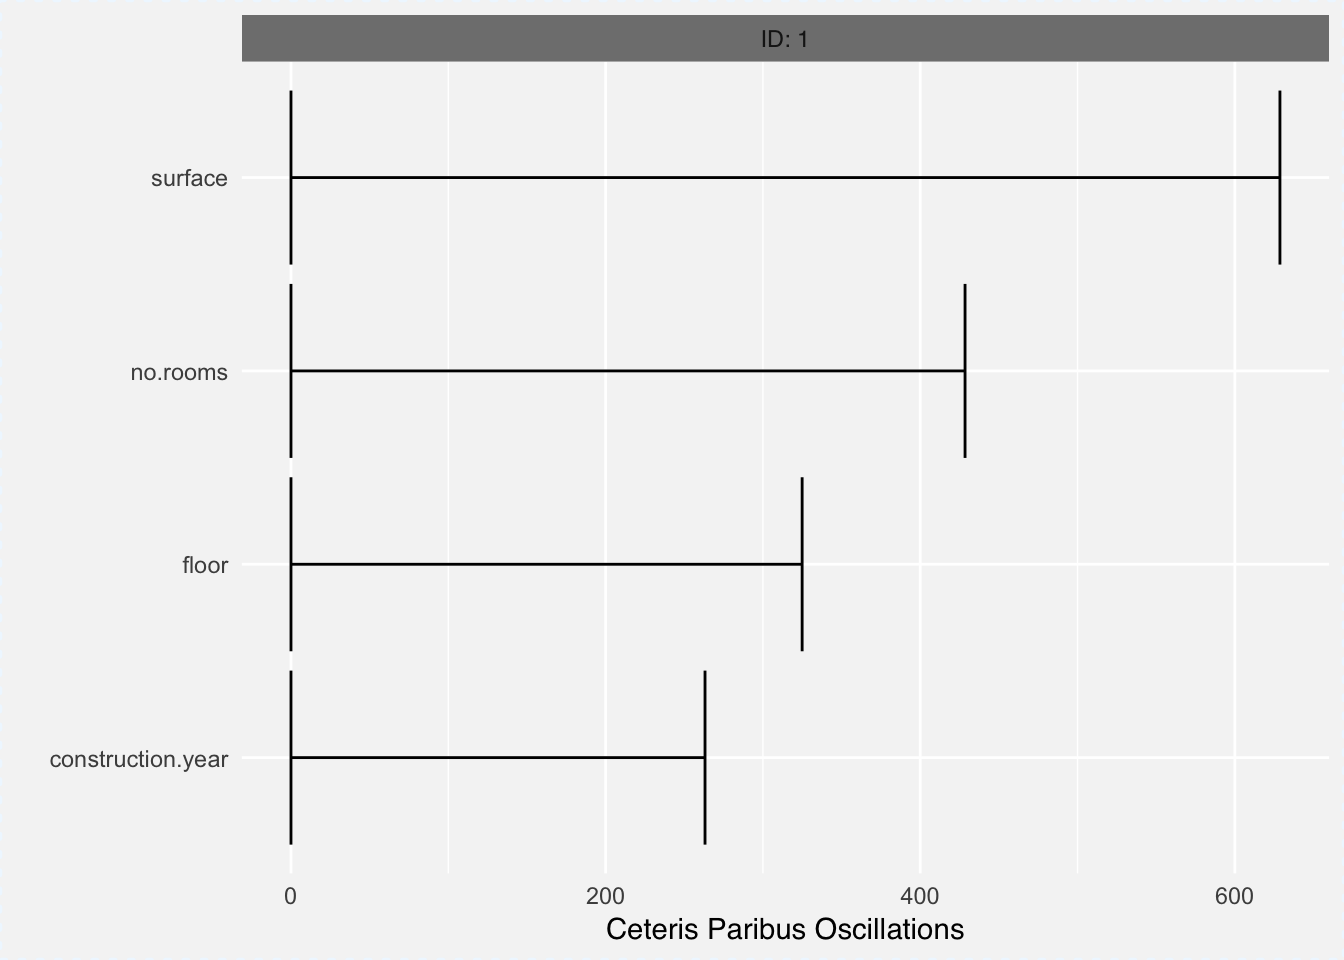
\includegraphics{PM_VEE_files/figure-latex/unnamed-chunk-35-1.pdf}

Almost all profiles behave in a similar way. The relation between age
and model response is on average decreasing for almost every neighbor.

\hypertarget{add-residuals-for-neighbors}{%
\subsubsection{Add residuals for
neighbors}\label{add-residuals-for-neighbors}}

And the last step is to add lines for residuals.

\begin{Shaded}
\begin{Highlighting}[]
\KeywordTok{plot}\NormalTok{(cp_johny) }\OperatorTok{+}
\StringTok{  }\KeywordTok{show_profiles}\NormalTok{(cp_johny_neighbors, }\DataTypeTok{color =} \StringTok{'#ceced9'}\NormalTok{) }\OperatorTok{+}\StringTok{ }
\StringTok{  }\KeywordTok{show_observations}\NormalTok{(cp_johny, }\DataTypeTok{variables =} \StringTok{"age"}\NormalTok{) }\OperatorTok{+}
\StringTok{  }\KeywordTok{show_residuals}\NormalTok{(cp_johny_neighbors, }\DataTypeTok{variables =} \StringTok{"age"}\NormalTok{) }\OperatorTok{+}
\StringTok{  }\KeywordTok{ggtitle}\NormalTok{(}\StringTok{"Local Fidelity Plot for Johnny D"}\NormalTok{,}\StringTok{"Calculated for titanic_rf_v6 model"}\NormalTok{)}
\end{Highlighting}
\end{Shaded}

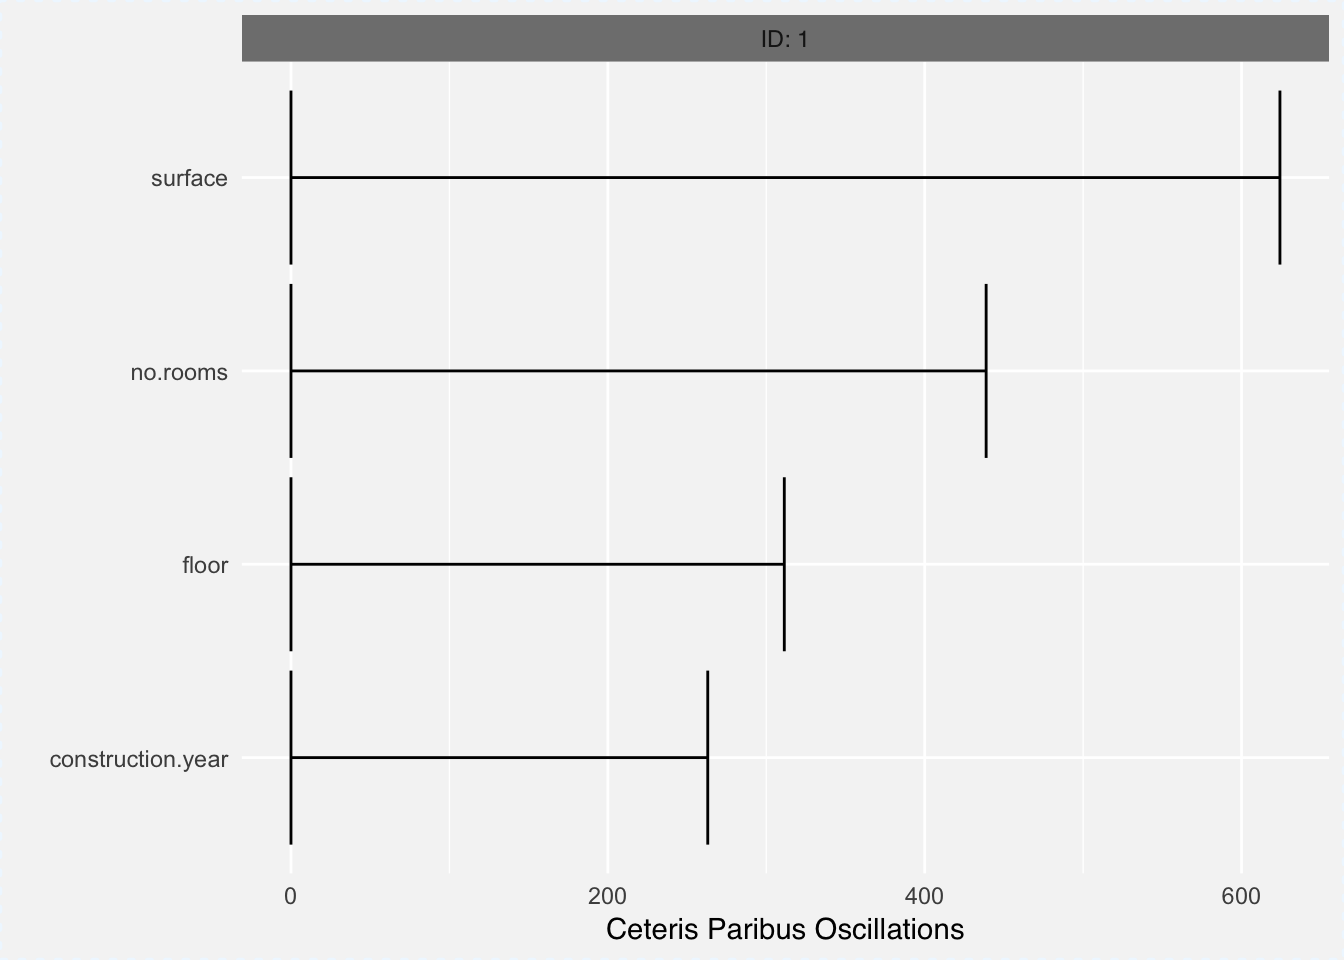
\includegraphics{PM_VEE_files/figure-latex/unnamed-chunk-36-1.pdf}

Added residuals works increase the trust in this model. Neighbors that
in fact died have lower profiles while neighbors that survived have
predictions higher than 50\%.

\hypertarget{variableAttributionMethods}{%
\section{Variable attribution for linear
models}\label{variableAttributionMethods}}

\hypertarget{introduction-5}{%
\subsection{Introduction}\label{introduction-5}}

In this chapter we introduce the concept and the intuitions underlying
`'variable attribution,'' i.e., the decomposition of the difference
between the single-instance and the average model predictions among the
different explanatory variables. We can think about the following
examples:

\begin{itemize}
\tightlist
\item
  Assume that we are interested in predicting the risk of heart attack
  based on person's age, sex, and smoking habits. A patient may want to
  know which factors have the highest impact on the his/her risk score.
\item
  Consider a model for prediction of apartment prices. An investor may
  want to know how much of the predicted price may be attributed to, for
  instance, the location of an apartment.
\item
  Consider a model for credit scoring. A customer may want to know if
  factors like gender, age, or number of children influence model
  predictions.
\end{itemize}

In each of those cases we want to attribute a part of the model
prediction to a single explanatory variable. This can be done directly
for linear models. Hence, in this chapter We focus on those models. The
method can be easily extended to generalized linear models.
Model-agnostic approaches will be presented in Chapters \ref{breakDown}
and \ref{shapley}.

\hypertarget{intuition-4}{%
\subsection{Intuition}\label{intuition-4}}

Assume a classical linear model for response \(Y\) with \(p\)
explanatory variables collected in the vector
\(X = (X_1, X_2, \ldots, X_p)\) and coefficients
\(\beta = (\beta_0, \beta_1, .., \beta_p)\), where \(\beta_0\) is the
intercept. The prediction for \(Y\) at point
\(X=x=(x_1, x_2, \ldots, x_p)\) is given by the expected value of \(Y\)
conditional on \(X=x\). For a linear model, the expected value is given
by the following linear combination:

\[
E_Y(Y | x) = f(x) = \beta_0 + x_1 \beta_1 + \ldots + x_p \beta_p.
\]\\
We are interested in the contribution of the \(i\)-th explanatory
variable to model prediction \(f(x^*)\) for a single observation
described by \(x^*\). In this case, the contribution is equal to
\(x^*_i\beta_i\), because the \(i\)-th variable occurs only in this
term. As it will become clear in the sequel, it is easier to interpret
the variable's contribution if \(x_i\) is is centered by subtracting a
constant \(\hat x_i\) (usually, the mean of \(x_i\)). This leads the
following, intuitive formula for the variable attribution: \[
v(f, x^*, i) = \beta_i (x_i^* - \hat x_i).
\]

\hypertarget{method-4}{%
\subsection{Method}\label{method-4}}

We want to calculate \(v(f, x^*, i)\), which is the contribution of the
\(i\)-th explanatory variable to the prediction of model \(f()\) at
point \(x^*\). Assume that \(E_Y(Y | x^*) \approx f(x^*)\), where
\(f(x^*)\) is the value of the model at \(x^*\). A possible approach to
define \(v(f, x^*, i)\) is to measure how much the expected model
response changes after conditioning on \(x_i^*\): \[
v(f, x^*, i) = E_Y(Y | x^*) - E_{X_i}\{E_Y[Y | (x_1^*,\ldots,x_{i-1}^*,X_i,x_{i+1}^*,x_p^*)]\}\approx f(x^*) - E_{X_i}[f(x_{-i}^*)],
\] where \(x_{-i}^*\) indicates that variable \(X_i\) in vector
\(x_{-i}^*\) is treated as random. For the classical linear model, if
the explanatory variables are independent, \(v(f, x^*, i)\) can be
expressed as follows: \[
v(f, x^*, i) = f(x^*) - E_{X_i}[f(x_{-i}^*)] = \beta_0 + x_1^* \beta_1 + \ldots + x_p^* \beta_p - E_{X_i}[\beta_0 + x_1^* \beta_1 + \ldots +\beta_i X_i \ldots + x_p^* \beta_p] = \beta_i[x^*_i - E_{X_i}(X_i)].
\] In practice, given a dataset, the expected value of \(X_i\) can be
estimated by the sample mean \(\bar x_i\). This leads to\\
\[
v(f, x^*, i) = \beta_i (x^*_i - \bar x_i).
\] Note that the linear-model-based prediction may be re-expressed in
the following way: \[
f(x^*) = [\beta_0 + \bar x_1 \beta_1 + ... + \bar x_p \beta_p] + [(x_1^* - \bar x_1) \beta_1 + ... + (x_p^* - \bar x_p) \beta_p] \equiv [average \ prediction] + \sum_{j=1}^p v(f, x^*, j).
\] Thus, the contributions of the explanatory variables are the
differences between the model prediction for \(x^*\) and the average
prediction.

** NOTE for careful readers **

Obviously, sample mean \(\bar x_i\) is an estimator of the expected
value \(E_{X_i}(X_i)\), calculated using a dataset. For the sake of
simplicity we do not emphasize these differences in the notation. Also,
we ignore the fact that, in practice, we never know the model
coefficients and we work with an estimated model.

Also, we assumed that the explanatory variables are independent, which
may not be the case. We will return to this problem in Section
{[}TOMASZ: INSERT REF{]}, when we will discuss interactions.

\hypertarget{example-wine-quality}{%
\subsection{Example: Wine quality}\label{example-wine-quality}}

Figure \ref{fig:attribution1a} shows the relation between alcohol and
wine quality, based on the wine dataset \citep{wine2009}. The linear
model is \[
quality(alcohol) = 2.5820 + 0.3135 * alcohol.
\] The weakest wine in the dataset has 8\% of alcohol, while the average
alcohol concentration is 10.51\%. Thus, the contribution of alcohol to
the model prediction for the weakest wine is
\(0.3135 \cdot (8-10.51) = -0.786885\). This means that low
concentration of alcohol for this wine (8\%) decreses the predicted
quality by \(-0.786885\).

Note, that it would be misleading to use
\(x_i^*\beta_i = 0.3135*8 = 2.508\) as the alcohol contribution to the
quality. The positive value of the product would not correrspond to the
intuition that, in the presence of a positive relation, a smaller
alcohol concentration should imply a lower quality of the wine.

\begin{figure}

{\centering 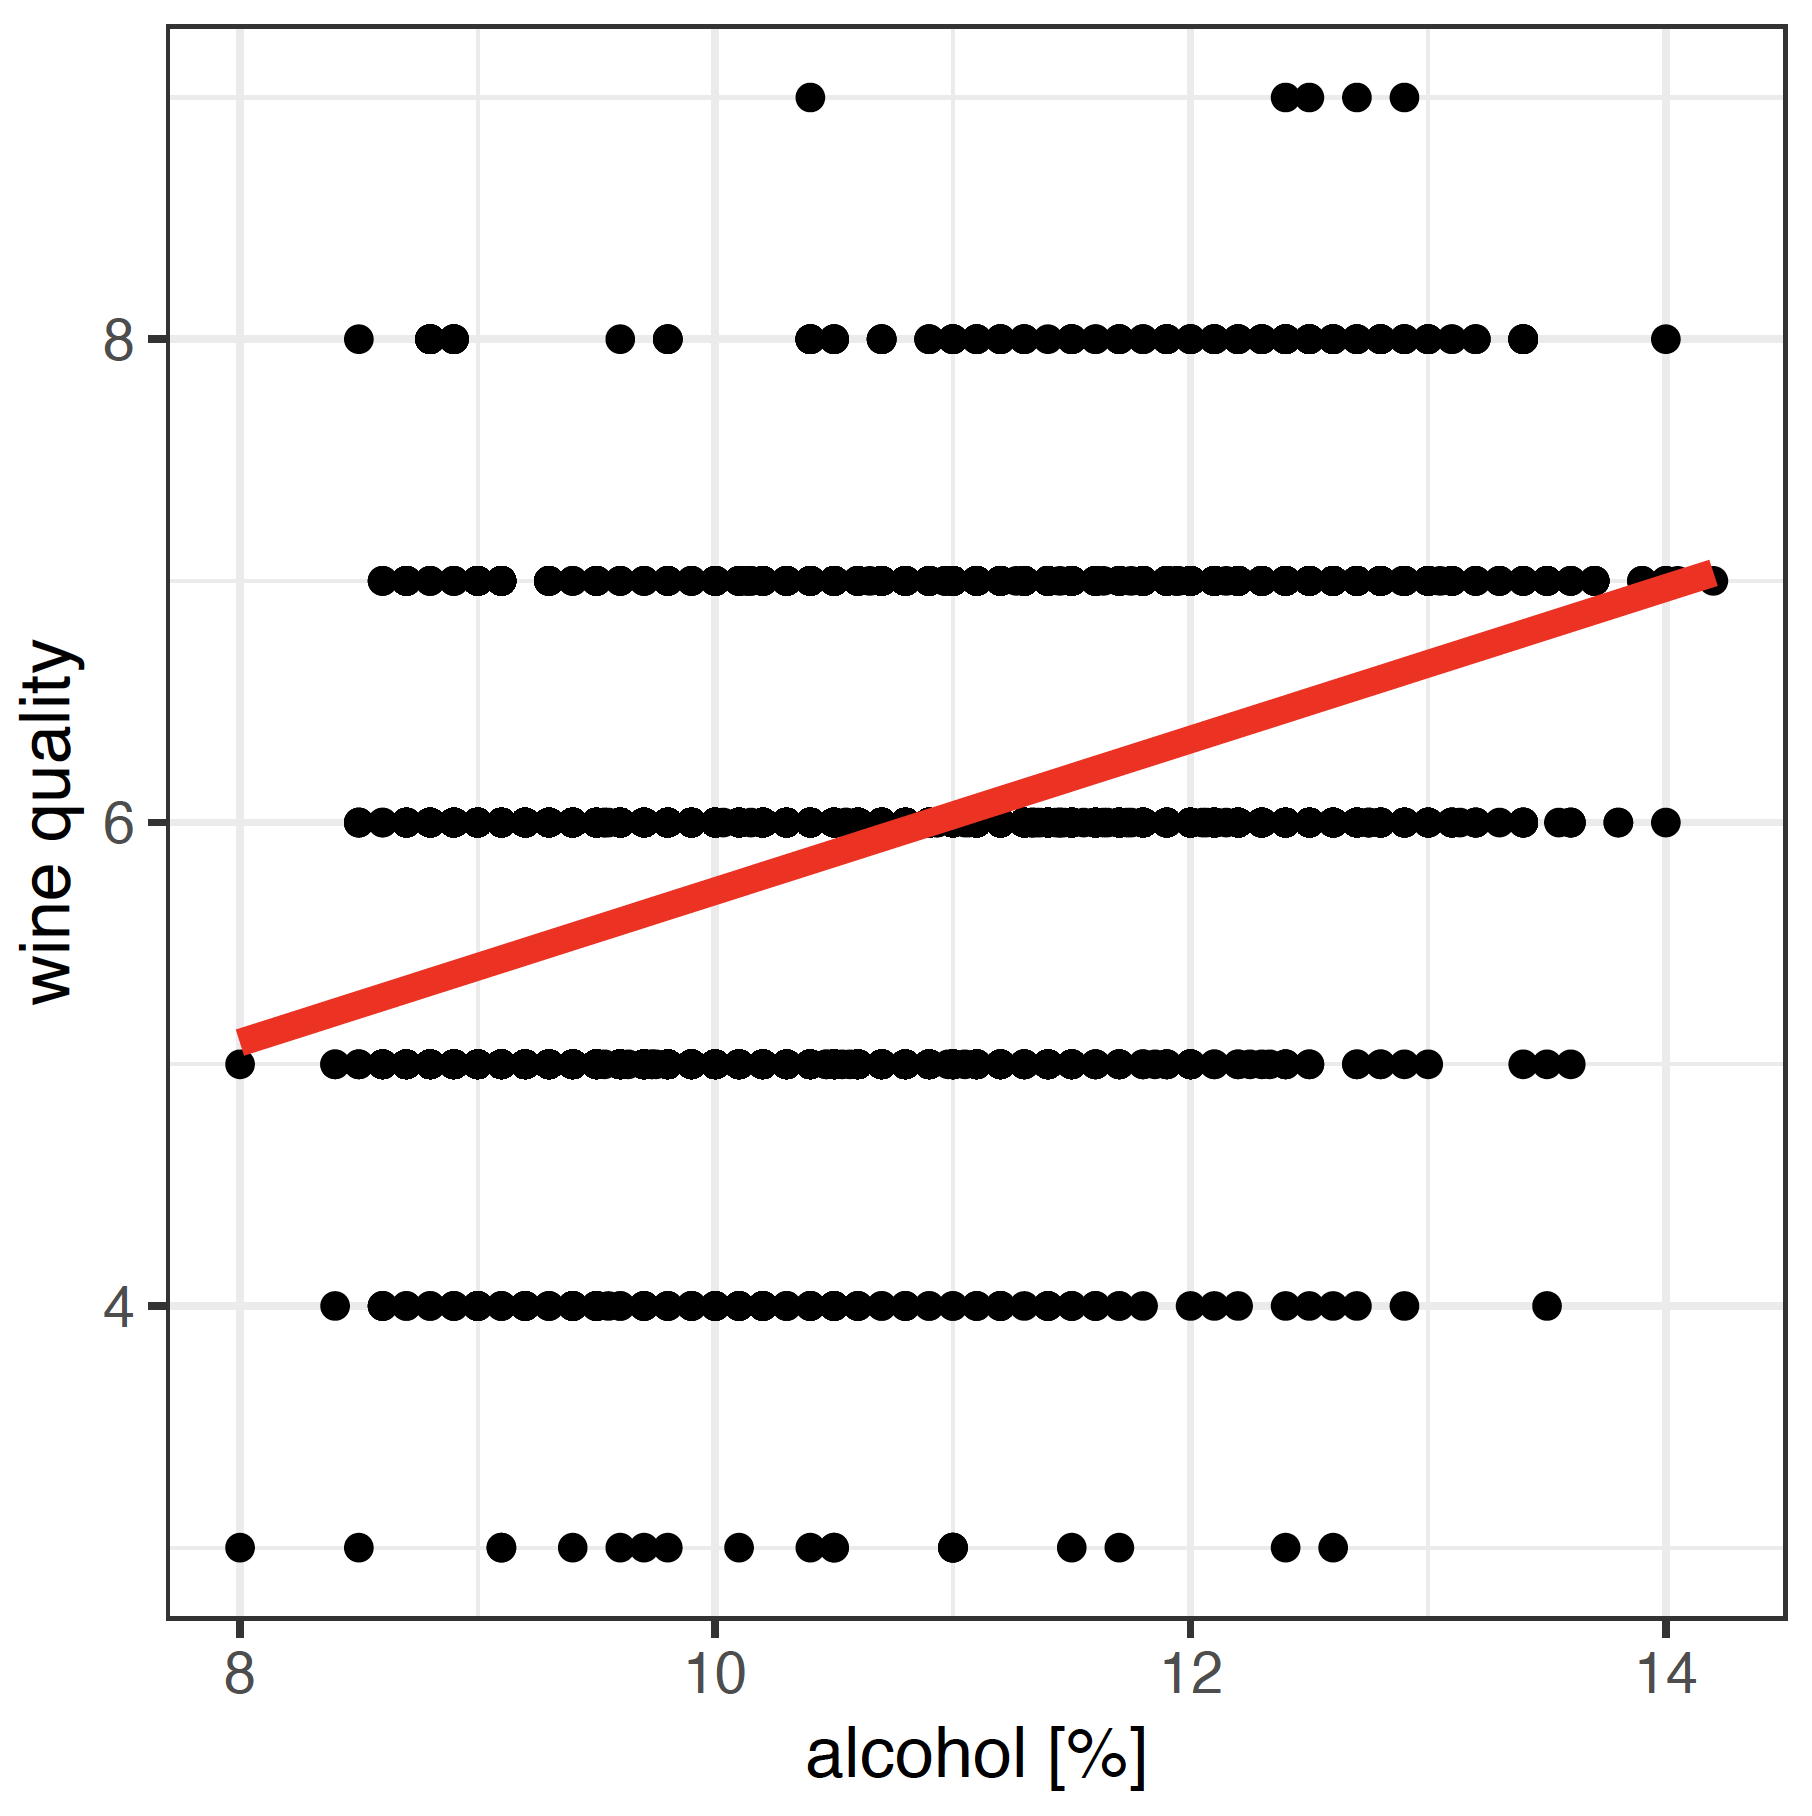
\includegraphics[width=0.5\linewidth]{figure/attribution_1} 

}

\caption{(fig:attribution1a)Relation between wine quality and concentration of alcohol assessed with linear model}\label{fig:attribution1a}
\end{figure}

\hypertarget{pros-and-cons-4}{%
\subsection{Pros and Cons}\label{pros-and-cons-4}}

The proposed definition of \(v(f, x^*, i)\) is linked neither with scale
nor location of \(X_i\); hence, it is easier to understand than, for
instance, the standardized value of \(\beta_i\). {[}TOMASZ: I AM NOT
SURE ABOUT THIS ARGUMENT. THE DEFINITION OF v() INVOLVES CENTERING.{]}
For the classical linear model, \(v(f, x^*, i)\) is not an approximation
and it is directly linked with the structure of a model. An obvious
diasadvantage is that the definition of \(v(f, x^*, i)\) is very much
linear-model based. Also, it does not, in any way, reduce the model
complexity; it only presents model coefficients in a different way.
{[}TOMASZ: I AM NOT SURE ABOUT THIS ARGUMENT. MODEL COMPLEXITY IS WHAT
IT IS. HOW CAN WE REDUCE IT?{]}

\hypertarget{code-snippets-1}{%
\subsection{Code snippets}\label{code-snippets-1}}

In this section, we present an example of computing variable
attributions using the \texttt{HR} dataset (see Section \ref{HRdataset}
for more details).

To calculate variable attributions for a particular point, first we have
got to define this point:

\begin{Shaded}
\begin{Highlighting}[]
\NormalTok{new_observation <-}\StringTok{ }\KeywordTok{data.frame}\NormalTok{(}\DataTypeTok{gender =} \KeywordTok{factor}\NormalTok{(}\StringTok{"male"}\NormalTok{, }\DataTypeTok{levels =} \KeywordTok{c}\NormalTok{(}\StringTok{"male"}\NormalTok{, }\StringTok{"female"}\NormalTok{)),}
                      \DataTypeTok{age =} \FloatTok{57.7}\NormalTok{,}
                      \DataTypeTok{hours =} \FloatTok{42.3}\NormalTok{,}
                      \DataTypeTok{evaluation =} \DecValTok{2}\NormalTok{,}
                      \DataTypeTok{salary =} \DecValTok{2}\NormalTok{)}
\end{Highlighting}
\end{Shaded}

Variable attributions for linear and generalized linear models may be
directly extracted by applying the \texttt{predict()} function, with the
argument \texttt{type\ =\ "terms"}, to an object containing results of
fitting of a model. To illustrate the approach for logistic regression,
we build a logistic regression model for the binary variable
\texttt{status\ ==\ "fired"} and extract the estimated model
coefficients:

\begin{Shaded}
\begin{Highlighting}[]
\KeywordTok{library}\NormalTok{(}\StringTok{"DALEX"}\NormalTok{)}
\NormalTok{model_fired <-}\StringTok{ }\KeywordTok{glm}\NormalTok{(status }\OperatorTok{==}\StringTok{ "fired"} \OperatorTok{~}\StringTok{ }\NormalTok{., }\DataTypeTok{data =}\NormalTok{ HR, }\DataTypeTok{family =} \StringTok{"binomial"}\NormalTok{)}
\KeywordTok{coef}\NormalTok{(model_fired)}
\end{Highlighting}
\end{Shaded}

\begin{verbatim}
##  (Intercept)   gendermale          age        hours   evaluation 
##  5.737945729 -0.066803609 -0.001503314 -0.102021120 -0.425793369 
##       salary 
## -0.015740080
\end{verbatim}

For the new observation, the predicted value of the logit of the
probability of being fired is obtained by applying the
\texttt{predict()} function:

\begin{Shaded}
\begin{Highlighting}[]
\KeywordTok{as.vector}\NormalTok{(pred.inst <-}\StringTok{ }\KeywordTok{predict}\NormalTok{(model_fired, new_observation)) }\CommentTok{# new pediction}
\end{Highlighting}
\end{Shaded}

\begin{verbatim}
## [1] 0.3858406
\end{verbatim}

On the other hand, variable attributions can be obtained by applying the
\texttt{predict()} function with the \texttt{type="terms"} argument:

\begin{Shaded}
\begin{Highlighting}[]
\NormalTok{(var.attr <-}\StringTok{ }\KeywordTok{predict}\NormalTok{(model_fired, new_observation, }\DataTypeTok{type =} \StringTok{"terms"}\NormalTok{)) }\CommentTok{# attributions}
\end{Highlighting}
\end{Shaded}

\begin{verbatim}
##        gender         age     hours evaluation      salary
## 1 -0.03361889 -0.02660691 0.7555555  0.5547197 0.007287334
## attr(,"constant")
## [1] -0.8714962
\end{verbatim}

The largest contributions to the prediction come from variables
`'hours'' and `'evaluation.'' Variables `'gender'' and `'age'' slightly
decrease the predicted value. The sum of the attributions is equal to

\begin{Shaded}
\begin{Highlighting}[]
\KeywordTok{sum}\NormalTok{(var.attr)}
\end{Highlighting}
\end{Shaded}

\begin{verbatim}
## [1] 1.257337
\end{verbatim}

The attribute \texttt{constant} of object \texttt{var.attr} provides the
`'average'' prediction, i.e., the predicted logit for an obsrvation
defined by the means of the explanatory variables, as can be seen from
the calculation below:

\begin{Shaded}
\begin{Highlighting}[]
\KeywordTok{coef}\NormalTok{(model_fired)}\OperatorTok\KeywordTok{c}\NormalTok{(}\DecValTok{1}\NormalTok{, }\KeywordTok{mean}\NormalTok{((HR}\OperatorTok{$}\NormalTok{gender}\OperatorTok{==}\StringTok{"male"}\NormalTok{)), }\KeywordTok{mean}\NormalTok{(HR}\OperatorTok{$}\NormalTok{age), }\KeywordTok{mean}\NormalTok{(HR}\OperatorTok{$}\NormalTok{hours), }
                      \KeywordTok{mean}\NormalTok{(HR}\OperatorTok{$}\NormalTok{evaluation), }\KeywordTok{mean}\NormalTok{(HR}\OperatorTok{$}\NormalTok{salary))}
\end{Highlighting}
\end{Shaded}

\begin{verbatim}
##            [,1]
## [1,] -0.8714962
\end{verbatim}

Adding the `'average'' prediction to the sum of the variable
attributions results in the new-observation prediction:

\begin{Shaded}
\begin{Highlighting}[]
\KeywordTok{attributes}\NormalTok{(var.attr)}\OperatorTok{$}\NormalTok{constant }\OperatorTok{+}\StringTok{ }\KeywordTok{sum}\NormalTok{(var.attr)}
\end{Highlighting}
\end{Shaded}

\begin{verbatim}
## [1] 0.3858406
\end{verbatim}

Below we illustrate how to implement this approach with the
\texttt{DALEX} package. Toward this end, functions \texttt{explain()}
and \texttt{single\_prediction()} can be used. Object
\texttt{model\_fired} stores the definition of the logistic-regression
model used earlier in this section. The contents of object
\texttt{attribution} correspond to the results obtained by using
function \texttt{predict()}.

\begin{Shaded}
\begin{Highlighting}[]
\KeywordTok{library}\NormalTok{(}\StringTok{"DALEX"}\NormalTok{)}

\NormalTok{explainer_fired <-}\StringTok{ }\KeywordTok{explain}\NormalTok{(model_fired,}
                 \DataTypeTok{data =}\NormalTok{ HR,}
                 \DataTypeTok{y =}\NormalTok{ HR}\OperatorTok{$}\NormalTok{status }\OperatorTok{==}\StringTok{ "fired"}\NormalTok{,}
                 \DataTypeTok{label =} \StringTok{"fired"}\NormalTok{)}

\NormalTok{(attribution <-}\StringTok{ }\KeywordTok{single_prediction}\NormalTok{(explainer_fired, new_observation))}
\end{Highlighting}
\end{Shaded}

\begin{verbatim}
##                    variable contribution variable_name variable_value
## 1               (Intercept) -0.871496150     Intercept              1
## hours        + hours = 42.3  0.755555494         hours           42.3
## evaluation + evaluation = 2  0.554719716    evaluation              2
## salary         + salary = 2  0.007287334        salary              2
## age            + age = 57.7 -0.026606908           age           57.7
## gender      + gender = male -0.033618893        gender           male
## 11          final_prognosis  0.385840593                             
##            cummulative sign position label
## 1           -0.8714962   -1        1 fired
## hours       -0.1159407    1        2 fired
## evaluation   0.4387791    1        3 fired
## salary       0.4460664    1        4 fired
## age          0.4194595   -1        5 fired
## gender       0.3858406   -1        6 fired
## 11           0.3858406    X        7 fired
\end{verbatim}

After object \texttt{attribution} has been created, a plot presenting
the variable attributions can be easily constructed:

\begin{Shaded}
\begin{Highlighting}[]
\KeywordTok{plot}\NormalTok{(attribution)}
\end{Highlighting}
\end{Shaded}

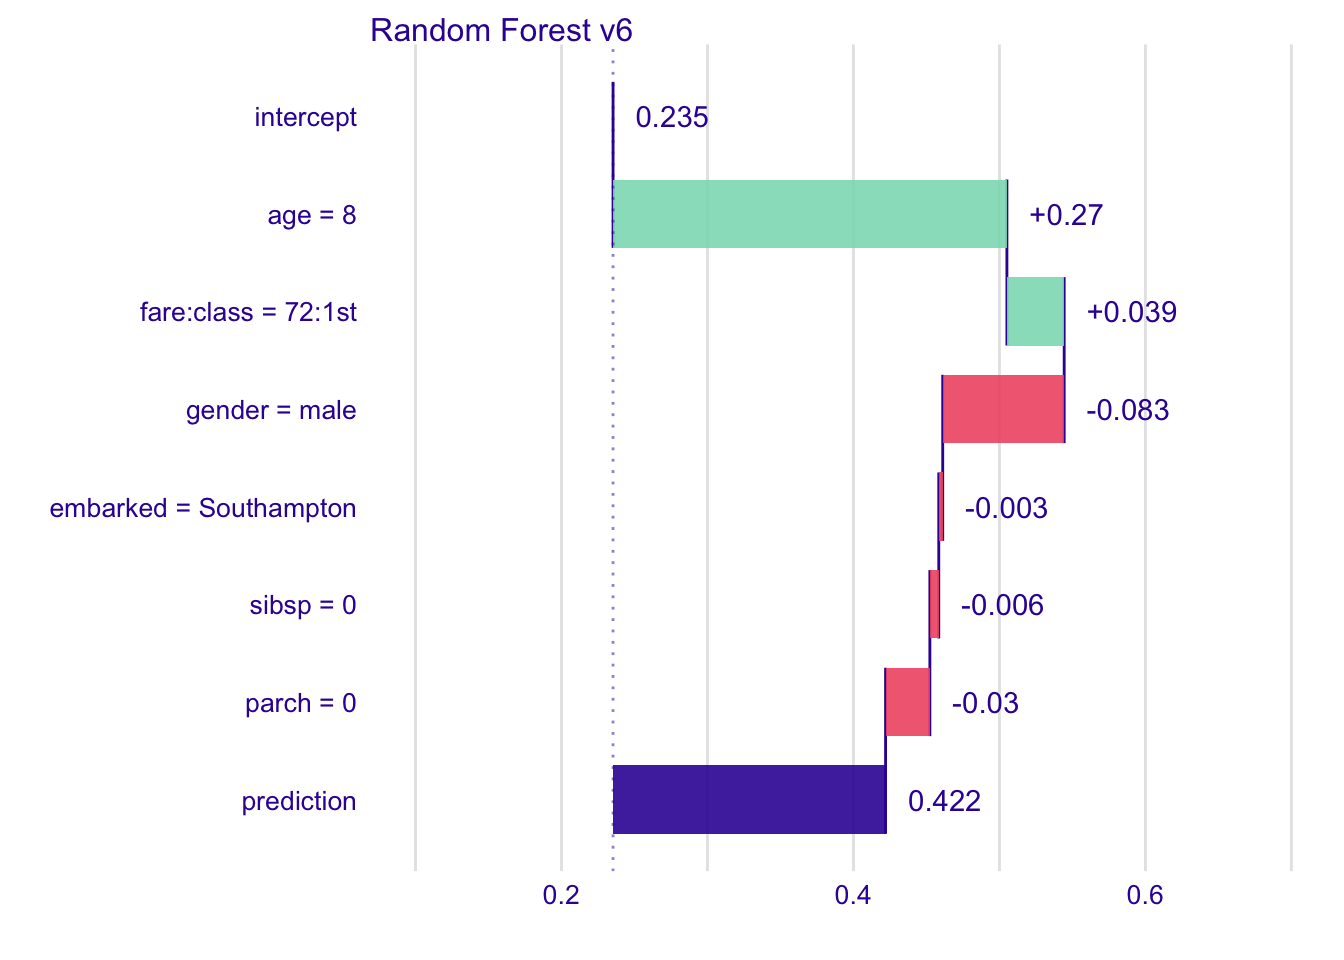
\includegraphics{PM_VEE_files/figure-latex/unnamed-chunk-45-1.pdf}

\hypertarget{breakDown}{%
\section{Variable attributions}\label{breakDown}}

In the Section \ref{variableAttributionMethods} we introduced a method
for calculation of variable attributions for linear models. This method
is accurate, based directly on the structure of the model. But for most
popular machine learning models we cannot assume that they are linear
nor even additive.

\hypertarget{intuition-5}{%
\subsection{Intuition}\label{intuition-5}}

For any model we may repeat the intuition presented in Section
\ref{variableAttributionMethods} to calculate variable contribution as
shifts in expected model response after conditioning over consecutive
variables. This intuition is presented in Figure \ref{BDPrice4}.

Panel A shows distribution of model responses. The row
\texttt{all\ data} shows the model response of the original dataset. The
red dot stands for average is is an estimate of expencted model response
\(E [f(x)]\).

Since we want to calculate effects of particular values of selected
variables we then condition over these variables in a sequential manner.
The next row in panel A corresponds to average model prediction for
observations with variable \texttt{surface} fixed to value \texttt{35}.
The next for corresponds to average model prediction with variables
\texttt{surface} set to \texttt{35} and \texttt{floor} set to
\texttt{1}, and so on. The top row corresponds to model response for
\(x^*\).

Black lines in the panel A show how prediction for a single point
changes after coordinate \(i\) is repaced by the \(x^*_i\). But finaly
we are not interestes in particular changes, not even in distributions
but only in averages - expected model responses.

The most minimal form that shows important information is presented in
the panel C. Positive values are presented with green bars while
negative differences are marked with yellow bar. They sum up to final
model prediction, which is denoted by a grey bar in this example.

\begin{figure}

{\centering 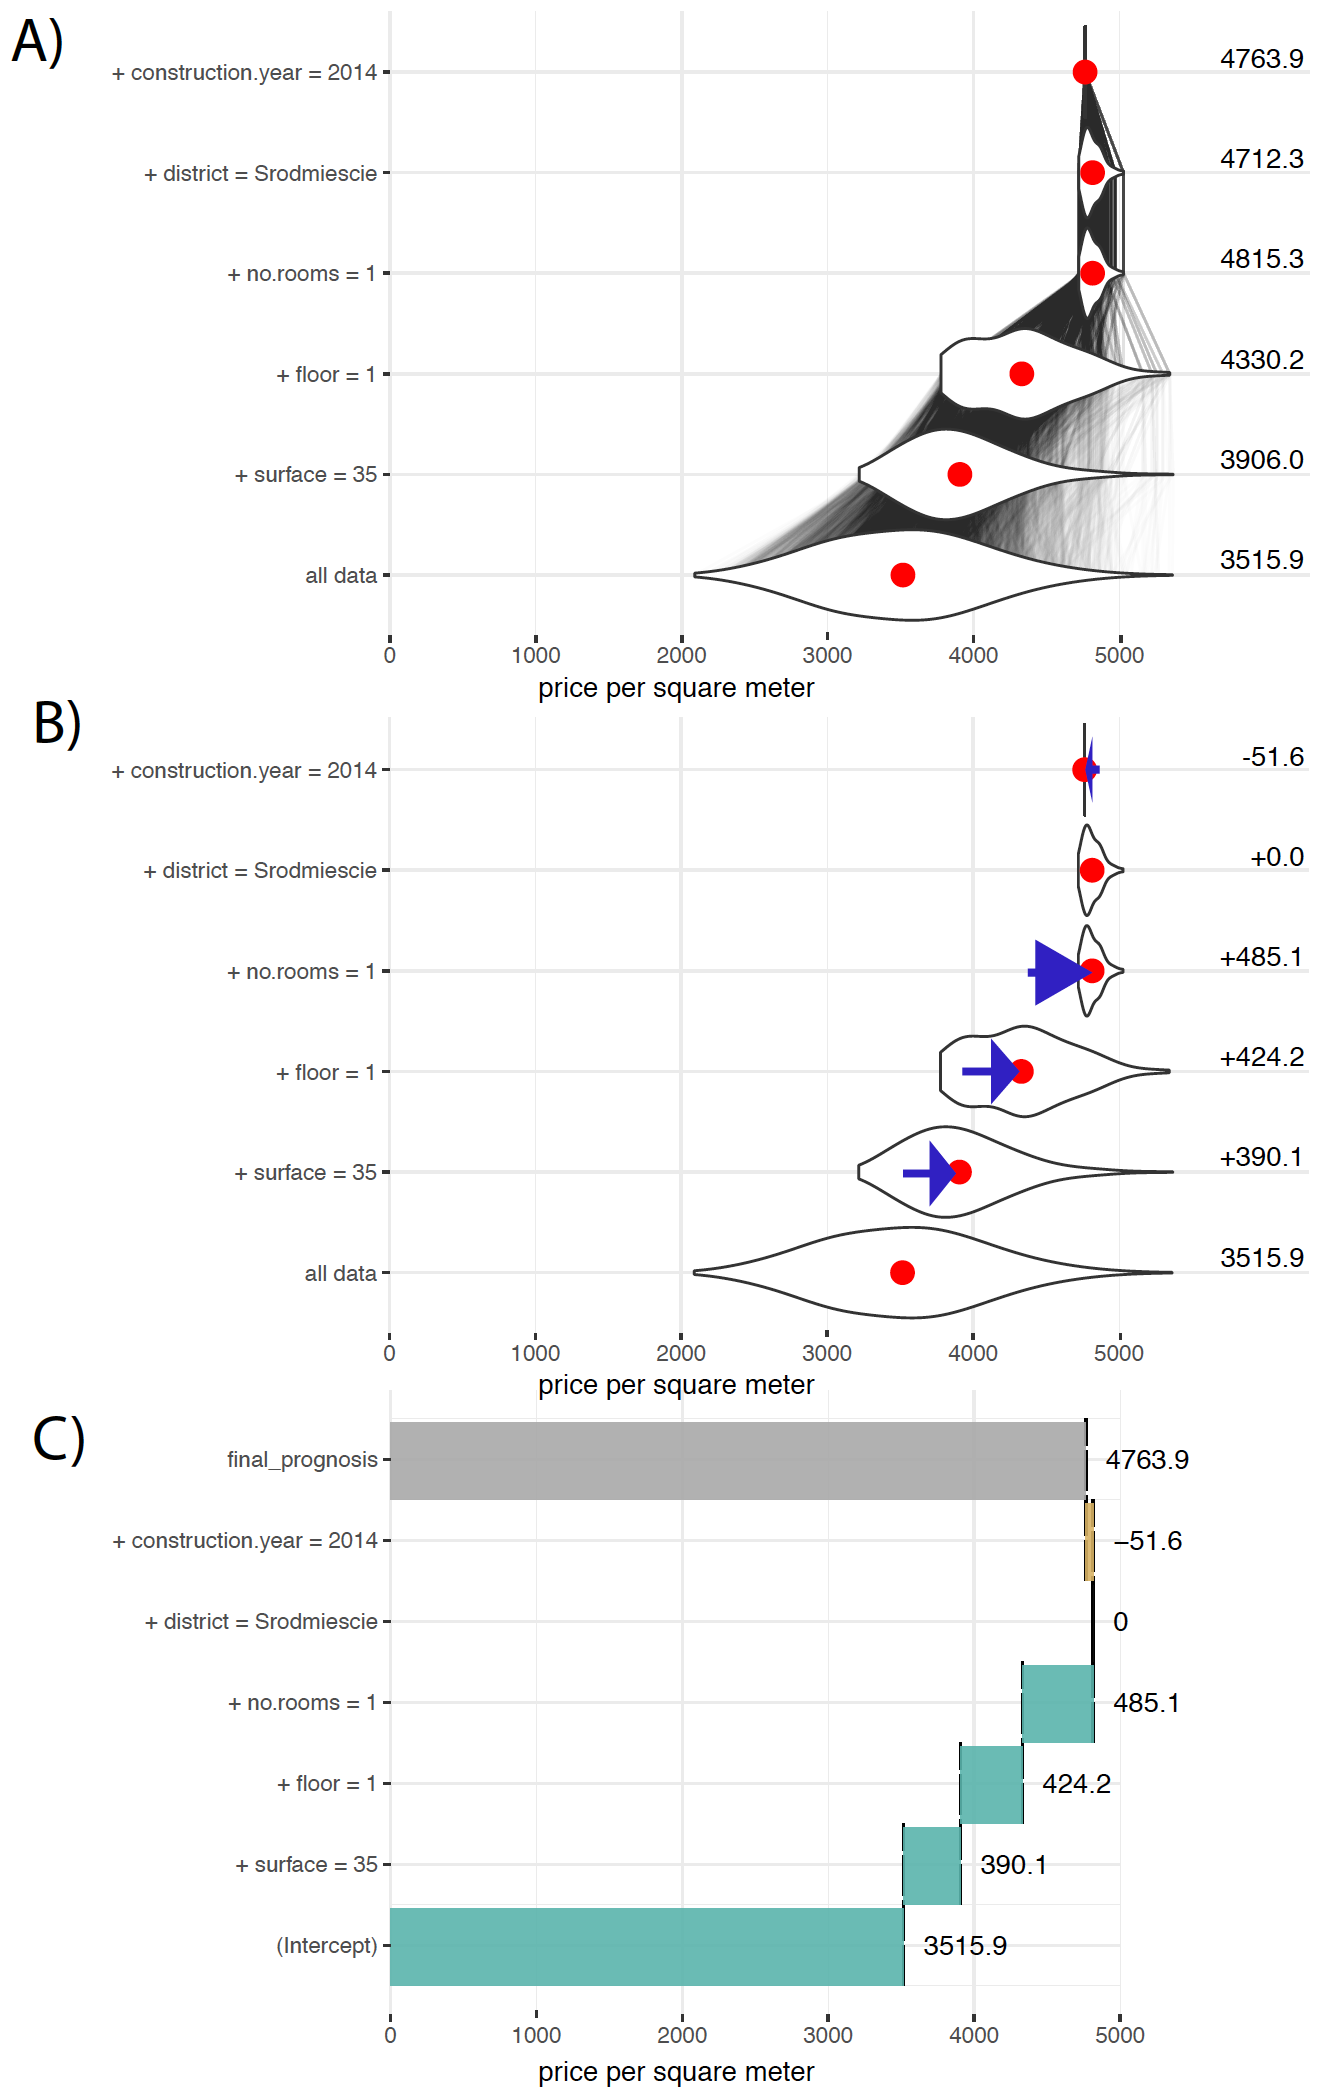
\includegraphics[width=0.7\linewidth]{figure/bd_price_4} 

}

\caption{(fig:BDPrice4) Break Down Plots show how variables move the model prediction from population average to the model prognosis for a single observation. A) The last row shows distribution of model predictions. Next rows show conditional distributions, every row a new variable is added to conditioning. The first row shows model prediction for a single point. Red dots stand for averages. B) Blue arrows shows how the average conditional response change, these values are variables contributions. C) Only variable contributions are presented. }\label{fig:BDPrice4}
\end{figure}

\hypertarget{method-5}{%
\subsection{Method}\label{method-5}}

Again, let \(v(f, x^*, i)\) stands for the contribution of variable
\(x_i\) on prediction of model \(f()\) in point \(x^*\).

We expect that such contribution will sum up to the model prediction in
a given point (property called \emph{local accuracy}), so \[
f(x^*) = baseline + \sum_{i=1}^p v(f, x^*, i)
\] where \(baseline\) stands for average model response.

Note that the equation above may be rewritten as

\[
E [f(X)|X_1 = x_1^*, \ldots, X+p = x_p^*] = E[f(X)] + \sum_{i=1}^p v(f, x^*, i)
\] what leads to quite natural proposition for \(v(f, x^*_i, i)\), such
as

\[
v(f, x^*_i, i) = E [f(X) | X_1 = x_1^*, \ldots, X_i = x_i^*] - E [f(X) | X_1 = x_1^*, \ldots, X_{i-1} = x_{i-1}^*] 
\] In other words the contribution of variable \(i\) is the difference
between expected model response conditioned on first \(i\) variables
minus the model response conditioned on first \(i-1\) variables.

Such proposition fulfills the \emph{local accuracy} condition, but
unfortunatelly variable contributions depends on the ordering of
variables.

\begin{figure}

{\centering 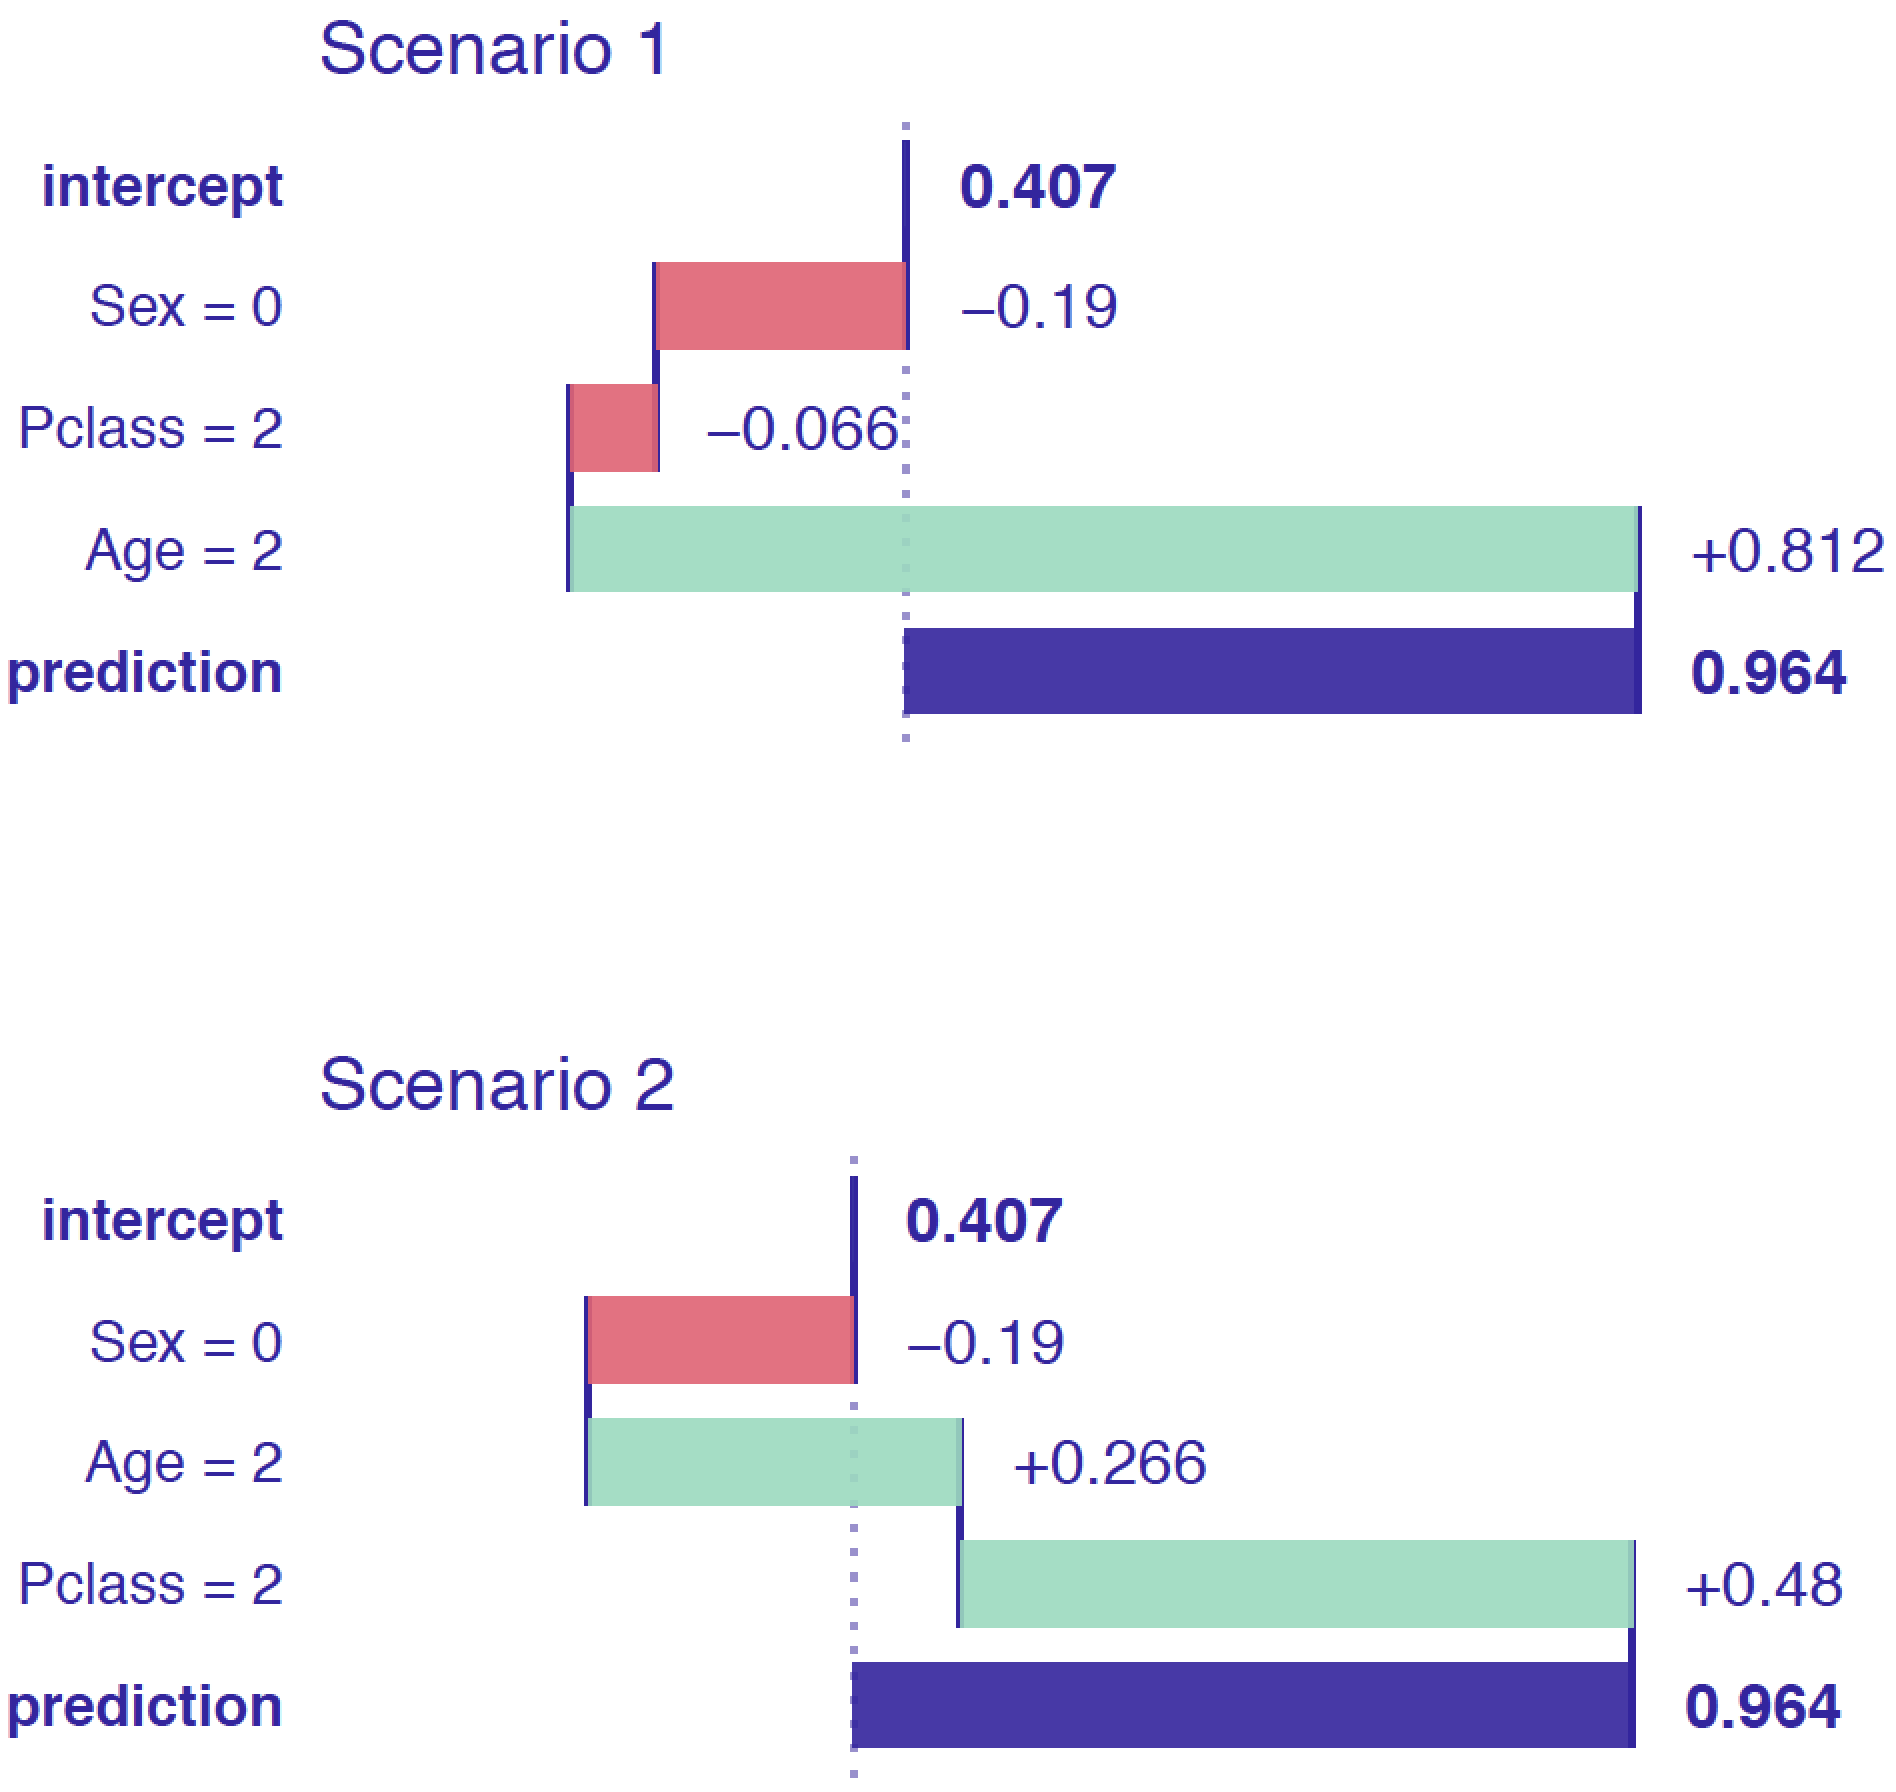
\includegraphics[width=1\linewidth]{figure/ordering} 

}

\caption{(fig:ordering) Two different paths between average model prediction and the model prediction for a selected observation. Black dots stand for conditional average, red arrows stands for changes between conditional averages.}\label{fig:ordering}
\end{figure}

See for example Figure \ref{fig:ordering}. In the first ordering the
contribution of variable \texttt{age} is calculated as 0.01, while in
the second the contribution is calculated as 0.13. Such differences are
related to the lack of additivness of the model \(f()\). Propositions
presented in next two sections present different solutions for this
problem.

The approach for variable attribution presented in the Section
\ref{modelAgnosticAttribution} has the property of \emph{local
accuracy}, but variable contributions depends on the variable ordering.

The easiest way to solve this problem is to use two-step procedure. In
the first step variables are ordered and in the second step the
consecutive conditioning is applied to ordered variables.

First step of this algorithm is to determine the order of variables for
conditioning. It seems to be reasonable to include first variables that
are likely to be most important, leaving the noise variables at the end.
This leads to order based on following scores

\[
score(f, x^*, i) = \left| E [f(X)] - E [f(X)|X_i = x^*_i] \right|
\] Note, that the absolute value is needed as variable contributions can
be both positive and negative.

Once the ordering is determined in the second step variable
contributions are calculated as

\[
v(f, x^*_i, i) = E [f(X) | X_{I \cup \{i\}} = x_{I \cup \{i\}}^*] - E [f(X) | X_{I} = x_{I}^*] 
\] where \(I\) is the set of variables that have scores smaller than
score for variable \(i\).

\[
I = \{j: score(f, x^*, j) < score(f, x^*, i)\}
\]

The time complexity of the first step id \(O(p)\) where \(p\) is the
number of variables and the time complexity of the second step is also
\(O(p)\).

\hypertarget{example-hire-or-fire}{%
\subsection{Example: Hire or Fire?}\label{example-hire-or-fire}}

Let us consider a random forest model created for HR data. The average
model response is \(\bar f(x) = 0.385586\). For a selected observation
\(x^*\) the table below presents scores for particular variables.

\begin{longtable}[]{@{}lrr@{}}
\toprule
& Ei f(X) & scorei\tabularnewline
\midrule
\endhead
hours & 0.616200 & 0.230614\tabularnewline
salary & 0.225528 & 0.160058\tabularnewline
evaluation & 0.430994 & 0.045408\tabularnewline
age & 0.364258 & 0.021328\tabularnewline
gender & 0.391060 & 0.005474\tabularnewline
\bottomrule
\end{longtable}

Once we determine the order we can calculate sequential contributions

\begin{longtable}[]{@{}lrr@{}}
\toprule
variable & cumulative & contribution\tabularnewline
\midrule
\endhead
(Intercept) & 0.385586 & 0.385586\tabularnewline
* hours = 42 & 0.616200 & 0.230614\tabularnewline
* salary = 2 & 0.400206 & -0.215994\tabularnewline
* evaluation = 2 & 0.405776 & 0.005570\tabularnewline
* age = 58 & 0.497314 & 0.091538\tabularnewline
* gender = male & 0.778000 & 0.280686\tabularnewline
final\_prognosis & 0.778000 & 0.778000\tabularnewline
\bottomrule
\end{longtable}

\hypertarget{pros-and-cons-5}{%
\subsection{Pros and cons}\label{pros-and-cons-5}}

Break Down approach is model agnostic, can be applied to any predictive
model that returns a single number. It leads to additive variable
attribution. Below we summarize key strengths and weaknesses of this
approach.

\textbf{Pros}

\begin{itemize}
\tightlist
\item
  Break Down Plots are easy to understand and decipher.
\item
  Break Down Plots are compact; many variables may be presented in a
  small space.
\item
  Break Down Plots are model agnostic yet they reduce to intuitive
  interpretation for linear Gaussian and generalized models.
\item
  Complexity of Break Down Algorithm is linear in respect to the number
  of variables.
\end{itemize}

\textbf{Cons}

\begin{itemize}
\tightlist
\item
  If the model is non-additive then showing only additive contributions
  may be misleading.
\item
  Selection of the ordering based on scores is subjective. Different
  orderings may lead to different contributions.
\item
  For large number of variables the Break Down Plot may be messy with
  many variables having small contributions.
\end{itemize}

\hypertarget{code-snippets-for-r-4}{%
\subsection{Code snippets for R}\label{code-snippets-for-r-4}}

In this section we present key features of the \texttt{breakDown2}
package for R \citep{R-breakDown}. This package covers all features
presented in this chapter. It is available on CRAN and GitHub. Find more
examples at the website of this package
\texttt{https://pbiecek.github.io/breakDown2/}.

\textbf{Model preparation}

In this section we will present an example based on the \texttt{HR}
dataset and Random Forest model \citep{R-randomForest}. See the Section
\ref{HRdataset} for more details.

\begin{Shaded}
\begin{Highlighting}[]
\KeywordTok{library}\NormalTok{(}\StringTok{"DALEX2"}\NormalTok{)}
\KeywordTok{library}\NormalTok{(}\StringTok{"randomForest"}\NormalTok{)}
\NormalTok{model <-}\StringTok{ }\KeywordTok{randomForest}\NormalTok{(status }\OperatorTok{~}\StringTok{ }\NormalTok{gender }\OperatorTok{+}\StringTok{ }\NormalTok{age }\OperatorTok{+}\StringTok{ }\NormalTok{hours }\OperatorTok{+}\StringTok{ }\NormalTok{evaluation }\OperatorTok{+}\StringTok{ }\NormalTok{salary, }\DataTypeTok{data =}\NormalTok{ HR)}
\NormalTok{model}
\end{Highlighting}
\end{Shaded}

\begin{verbatim}
## 
## Call:
##  randomForest(formula = status ~ gender + age + hours + evaluation +      salary, data = HR) 
##                Type of random forest: classification
##                      Number of trees: 500
## No. of variables tried at each split: 2
## 
##         OOB estimate of  error rate: 27.41%
## Confusion matrix:
##          fired   ok promoted class.error
## fired     2276  385      194   0.2028021
## ok         540 1250      431   0.4371905
## promoted   208  393     2170   0.2168892
\end{verbatim}

Model exploration with the \texttt{breakDown2} package is performed in
three steps.

\textbf{1. Create an explainer - wrapper around model and validation
data.}

Since all other functions work in a model agnostic fashion, first we
need to define a wrapper around the model. Here we are using the
\texttt{explain()} function from \texttt{DALEX2} package
\citep{R-DALEX}.

\begin{Shaded}
\begin{Highlighting}[]
\NormalTok{explainer_rf <-}\StringTok{ }\KeywordTok{explain}\NormalTok{(model,}
                 \DataTypeTok{data =}\NormalTok{ HR,}
                 \DataTypeTok{y =}\NormalTok{ HR}\OperatorTok{$}\NormalTok{status)}
\end{Highlighting}
\end{Shaded}

\textbf{2. Select an observation of interest.}

Break Down Plots decompose model prediction around a single observation.
Let's construct a data frame with corresponding values.

\begin{Shaded}
\begin{Highlighting}[]
\NormalTok{new_observation <-}\StringTok{ }\KeywordTok{data.frame}\NormalTok{(}\DataTypeTok{gender =} \KeywordTok{factor}\NormalTok{(}\StringTok{"male"}\NormalTok{, }\DataTypeTok{levels =} \KeywordTok{c}\NormalTok{(}\StringTok{"male"}\NormalTok{, }\StringTok{"female"}\NormalTok{)),}
                      \DataTypeTok{age =} \FloatTok{57.7}\NormalTok{,}
                      \DataTypeTok{hours =} \FloatTok{42.3}\NormalTok{,}
                      \DataTypeTok{evaluation =} \DecValTok{2}\NormalTok{,}
                      \DataTypeTok{salary =} \DecValTok{2}\NormalTok{)}

\KeywordTok{predict}\NormalTok{(model, new_observation, }\DataTypeTok{type =} \StringTok{"prob"}\NormalTok{)}
\end{Highlighting}
\end{Shaded}

\begin{verbatim}
##   fired    ok promoted
## 1 0.778 0.222        0
## attr(,"class")
## [1] "matrix" "votes"
\end{verbatim}

\textbf{3. Calculate Break Down decomposition}

The \texttt{local\_attributions()} function calculates Break Down
contributions for a selected model around a selected observation.

The result from \texttt{local\_attributions()} function is a data frame
with variable attributions.

\begin{Shaded}
\begin{Highlighting}[]
\KeywordTok{library}\NormalTok{(}\StringTok{"iBreakDown"}\NormalTok{)}
\NormalTok{bd_rf <-}\StringTok{ }\KeywordTok{local_attributions}\NormalTok{(explainer_rf,}
\NormalTok{                 new_observation,}
                 \DataTypeTok{keep_distributions =} \OtherTok{TRUE}\NormalTok{)}

\NormalTok{bd_rf}
\end{Highlighting}
\end{Shaded}

\begin{verbatim}
##                                       contribution
## randomForest.fired: intercept                0.376
## randomForest.fired: hours = 42               0.240
## randomForest.fired: evaluation = 2           0.062
## randomForest.fired: salary = 2              -0.251
## randomForest.fired: age = 58                 0.077
## randomForest.fired: gender = male            0.274
## randomForest.fired: prediction               0.778
## randomForest.ok: intercept                   0.276
## randomForest.ok: hours = 42                 -0.046
## randomForest.ok: evaluation = 2              0.086
## randomForest.ok: salary = 2                  0.248
## randomForest.ok: age = 58                   -0.069
## randomForest.ok: gender = male              -0.274
## randomForest.ok: prediction                  0.222
## randomForest.promoted: intercept             0.348
## randomForest.promoted: hours = 42           -0.194
## randomForest.promoted: evaluation = 2       -0.148
## randomForest.promoted: salary = 2            0.002
## randomForest.promoted: age = 58             -0.009
## randomForest.promoted: gender = male         0.000
## randomForest.promoted: prediction            0.000
\end{verbatim}

The generic \texttt{plot()} function creates a Break Down plots.

\begin{Shaded}
\begin{Highlighting}[]
\KeywordTok{plot}\NormalTok{(bd_rf) }
\end{Highlighting}
\end{Shaded}

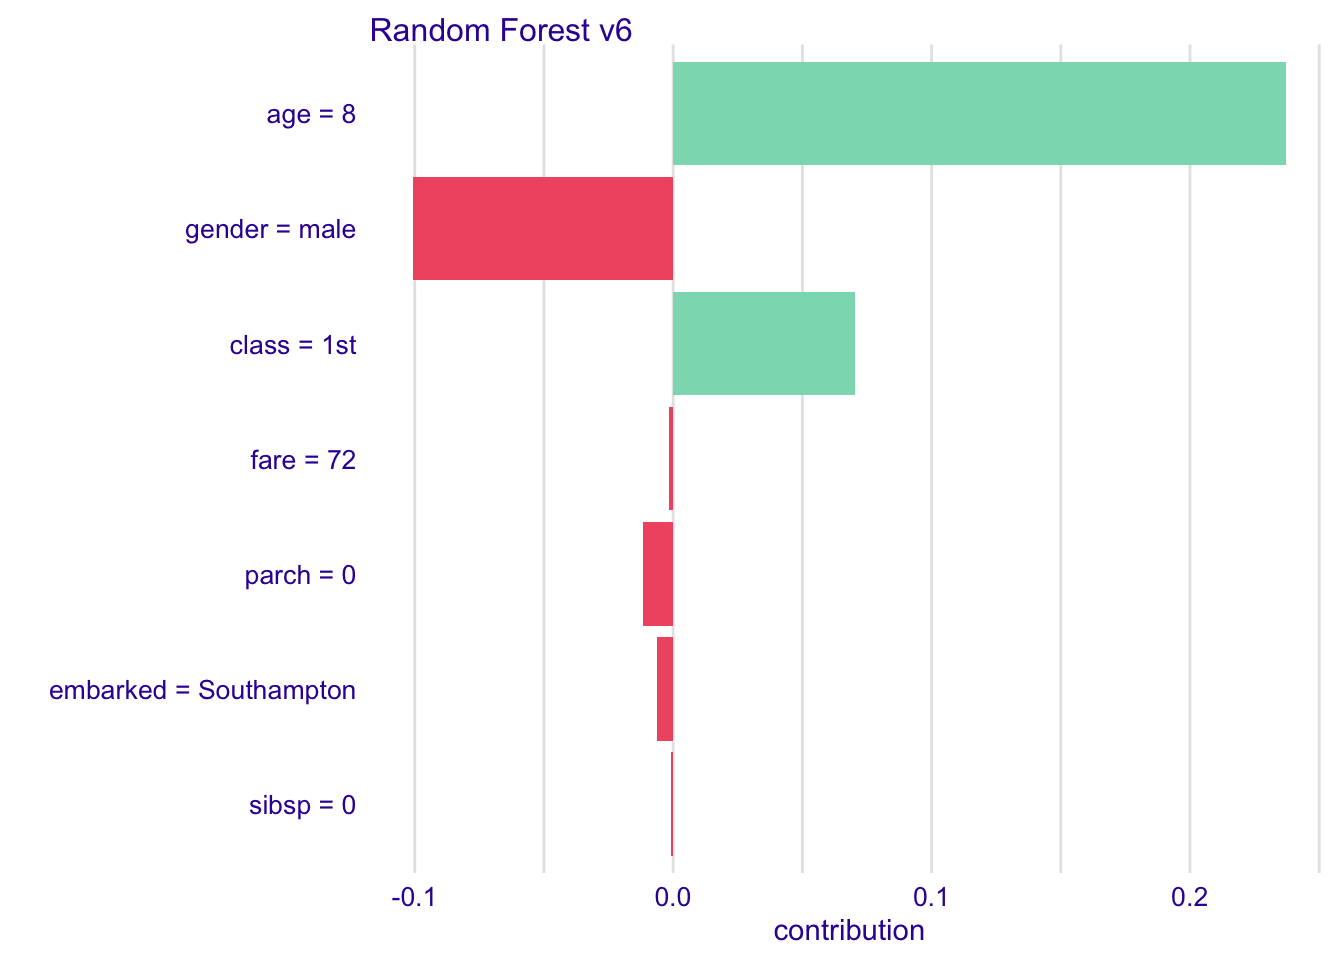
\includegraphics{PM_VEE_files/figure-latex/unnamed-chunk-50-1.pdf}

Add the \texttt{plot\_distributions\ =\ TRUE} argument to enrich model
response with additional information.

\begin{Shaded}
\begin{Highlighting}[]
\KeywordTok{plot}\NormalTok{(bd_rf, }\DataTypeTok{plot_distributions =} \OtherTok{TRUE}\NormalTok{) }
\end{Highlighting}
\end{Shaded}

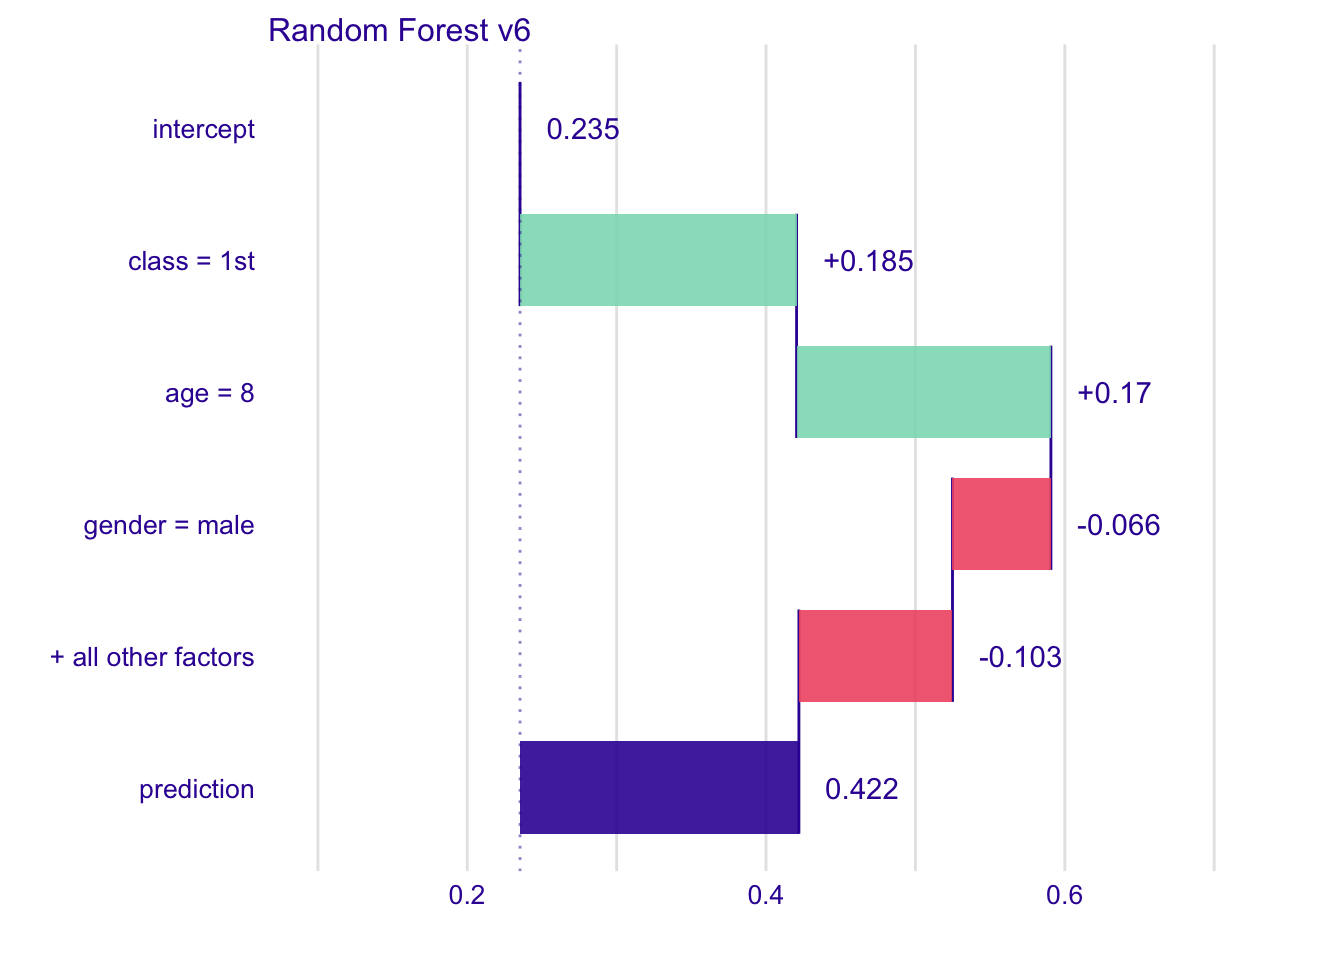
\includegraphics{PM_VEE_files/figure-latex/unnamed-chunk-51-1.pdf}

\hypertarget{variable-attribution-with-interactions}{%
\section{Variable attribution with
interactions}\label{variable-attribution-with-interactions}}

In the Section \ref{breakDown} we presented model agnostic approach for
additive decomposition of a model prediction for a single observation.

For non-additive models the variables contributions depend on values of
other variables.

In this section we present an algorithm that identifies interactions
between pairs of variables and include such interactions in variable
decomposition plots. Here we present an algorithm for pairs of
variables, but it can be easily generalized to larger number of
variables.

\hypertarget{intuition-6}{%
\subsection{Intuition}\label{intuition-6}}

The key idea here is to identify interactions between variables. This
can be done in two steps.

\begin{enumerate}
\def\labelenumi{\arabic{enumi}.}
\tightlist
\item
  First we determine variable contributions for each variable
  independently.
\item
  Second, we calculate effect for pair of variables. If this effect is
  different than the sum of consecutive variables then it may be an
  interaction.
\end{enumerate}

TODO: easy example for interaction

\hypertarget{method-6}{%
\subsection{Method}\label{method-6}}

This algorithm is also composed out of two steps. In the first step
variables and pairs of variables are ordered in terms of their
importance, while in the second step the consecutive conditioning is
applied to ordered variables.

To determine an importance of variables and pairs of variables following
scores are being calculated.

For a single variable

\[
score_1(f, x^*, i) = \left| E [f(X)|X_i = x^*_i]  - E [f(X)]\right|
\] For pairs of variables

\[
score_2(f, x^*, (i,j)) = \left| E [f(X)|X_i = x^*_i, X_j = x^*_j] - E [f(X)|X_i = x^*_i] - E [f(X)| X_j = x^*_j]+ E [f(X)] \right|
\] Note that this is equivalent to

\[
score_2(f, x^*, (i,j)) = \left| E [f(X)|X_i = x^*_i, X_j = x^*_j] - score_1 (f, x^*, i) - score_1 (f, x^*, j) + baseline \right|
\] In other words the \(score_1(f, x^*, i)\) measures how much the
average model response changes if variable \(x_i\) is set to \(x_i^*\),
which is some index of local variable importance. On the other hand the
\(score_2(f, x^*, (i,j))\) measures how much the change is different
than additive composition of changes for \(x_i\) and \(x_j\), which is
some index of local interaction importance.

Note, that for additive models \(score_2(f, x^*, (i,j))\) shall be close
to zero. So the larger is this value the larger deviation from
additivness.

The second step of the algorithm is the sequential conditioning. In this
version in every new step we condition on a single variable of pair of
variables in an order determined by \(score_1\) and \(score_2\).

The complexity of the first step id \(O(p^2)\) where \(p\) stands for
the number of variables. The complexity of the second step is \(O(p)\).

\hypertarget{example-hire-or-fire-1}{%
\subsection{Example: Hire or Fire?}\label{example-hire-or-fire-1}}

Again, let us consider a HR dataset. The table below shows \(score_1\)
and \(score_2\) calculated for consecutive variables.

\begin{longtable}[]{@{}lrrr@{}}
\toprule
& Ei f(X) & score1 & score2\tabularnewline
\midrule
\endhead
hours & 0.616200 & 0.230614 &\tabularnewline
salary & 0.225528 & -0.160058 &\tabularnewline
age:gender & 0.516392 & & 0.146660\tabularnewline
salary:age & 0.266226 & & 0.062026\tabularnewline
salary:hours & 0.400206 & & -0.055936\tabularnewline
evaluation & 0.430994 & 0.045408 &\tabularnewline
hours:age & 0.635662 & & 0.040790\tabularnewline
salary:evaluation & 0.238126 & & -0.032810\tabularnewline
age & 0.364258 & -0.021328 &\tabularnewline
evaluation:hours & 0.677798 & & 0.016190\tabularnewline
salary:gender & 0.223292 & & -0.007710\tabularnewline
evaluation:age & 0.415688 & & 0.006022\tabularnewline
gender & 0.391060 & 0.005474 &\tabularnewline
hours:gender & 0.626478 & & 0.004804\tabularnewline
evaluation:gender & 0.433814 & & -0.002654\tabularnewline
\bottomrule
\end{longtable}

Once we determined the order, we can calculate sequential conditionings.
In the first step we condition over variable \texttt{hours}, then over
\texttt{salary}. The third position is occupied by interaction between
\texttt{age:gender} thus we add both variables to the conditioning

\begin{longtable}[]{@{}lrr@{}}
\toprule
variable & cumulative & contribution\tabularnewline
\midrule
\endhead
(Intercept) & 0.385586 & 0.385586\tabularnewline
* hours = 42 & 0.616200 & 0.230614\tabularnewline
* salary = 2 & 0.400206 & -0.215994\tabularnewline
* age:gender = 58:male & 0.796856 & 0.396650\tabularnewline
* evaluation = 2 & 0.778000 & -0.018856\tabularnewline
final\_prognosis & 0.778000 & 0.778000\tabularnewline
\bottomrule
\end{longtable}

\hypertarget{break-down-plots}{%
\subsection{Break Down Plots}\label{break-down-plots}}

Break Down Plots for interactions are similar in structure as plots for
single variables. The only difference is that in some rows pair of
variable is listed in a single row. See an example in Figure
\ref{BDPrice4}.

\begin{figure}

{\centering 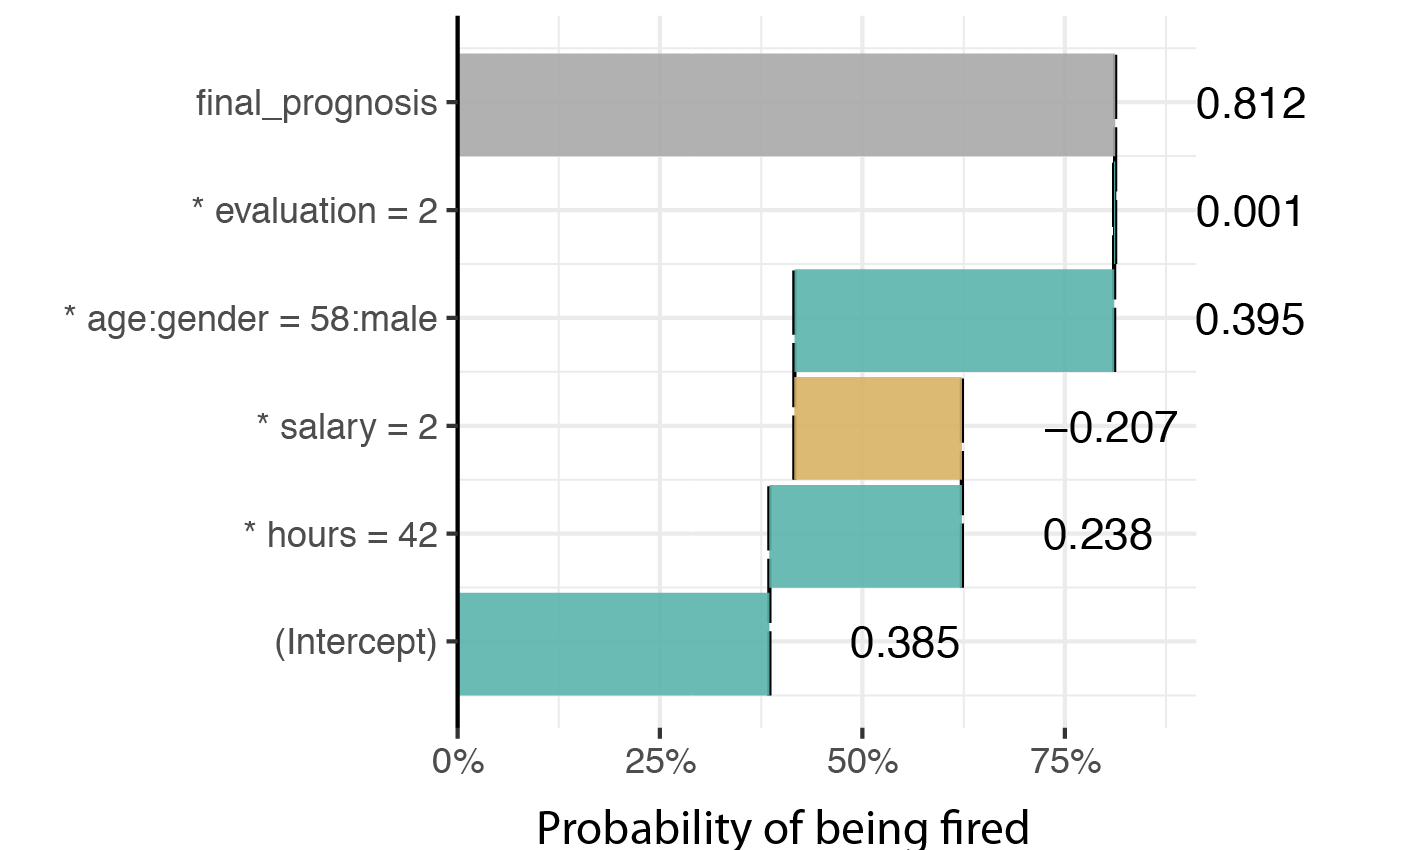
\includegraphics[width=0.7\linewidth]{figure/bd_inter_1} 

}

\caption{(fig:bdInter1) Break Down Plot for variable attrbution with interactions }\label{fig:bdInter1}
\end{figure}

\hypertarget{pros-and-cons-6}{%
\subsection{Pros and cons}\label{pros-and-cons-6}}

Break Down for interactions shares many features of Break Down for
single variables. Below we summarize unique strengths and weaknesses of
this approach.

\textbf{Pros}

\begin{itemize}
\tightlist
\item
  If interactions are present in the model, then additive contributions
  may be misleading. In such case the identification of interactions
  leads to better explanations.
\item
  Complexity of Break Down Algorithm is quadratic, what is not that bad
  if number of features is small or moderate.
\end{itemize}

\textbf{Cons}

\begin{itemize}
\tightlist
\item
  For large number of variables, the consideration of all interactions
  is both time consuming and sensitive to noise as the number of
  \(score_2\) scores grow faster than number of \(score_1\).
\end{itemize}

\hypertarget{code-snippets-for-r-5}{%
\subsection{Code snippets for R}\label{code-snippets-for-r-5}}

The algorithm for Break Down for Interactions is also implemented in the
\texttt{local\_interactions} function from \texttt{breakDown2} package.

\textbf{Model preparation}

First a model needs to be trained.

\begin{Shaded}
\begin{Highlighting}[]
\KeywordTok{library}\NormalTok{(}\StringTok{"DALEX2"}\NormalTok{)}
\KeywordTok{library}\NormalTok{(}\StringTok{"randomForest"}\NormalTok{)}
\NormalTok{model <-}\StringTok{ }\KeywordTok{randomForest}\NormalTok{(status }\OperatorTok{~}\StringTok{ }\NormalTok{gender }\OperatorTok{+}\StringTok{ }\NormalTok{age }\OperatorTok{+}\StringTok{ }\NormalTok{hours }\OperatorTok{+}\StringTok{ }\NormalTok{evaluation }\OperatorTok{+}\StringTok{ }\NormalTok{salary, }\DataTypeTok{data =}\NormalTok{ HR)}
\NormalTok{model}
\end{Highlighting}
\end{Shaded}

\begin{verbatim}
## 
## Call:
##  randomForest(formula = status ~ gender + age + hours + evaluation +      salary, data = HR) 
##                Type of random forest: classification
##                      Number of trees: 500
## No. of variables tried at each split: 2
## 
##         OOB estimate of  error rate: 27.37%
## Confusion matrix:
##          fired   ok promoted class.error
## fired     2259  388      208   0.2087566
## ok         523 1254      444   0.4353895
## promoted   199  386     2186   0.2111151
\end{verbatim}

Model exploration with the \texttt{breakDown2} package is performed in
three steps.

\textbf{1. Create an explainer - wrapper around model and validation
data.}

Since all other functions work in a model agnostic fashion, first we
need to define a wrapper around the model. Here we are using the
\texttt{explain()} function from \texttt{DALEX} package.

\begin{Shaded}
\begin{Highlighting}[]
\NormalTok{explainer_rf <-}\StringTok{ }\KeywordTok{explain}\NormalTok{(model,}
                 \DataTypeTok{data =}\NormalTok{ HR,}
                 \DataTypeTok{y =}\NormalTok{ HR}\OperatorTok{$}\NormalTok{status)}
\end{Highlighting}
\end{Shaded}

\textbf{2. Select an observation of interest.}

Break Down Plots decompose model prediction around a single observation.
Let's construct a data frame with corresponding values.

\begin{Shaded}
\begin{Highlighting}[]
\NormalTok{new_observation <-}\StringTok{ }\KeywordTok{data.frame}\NormalTok{(}\DataTypeTok{gender =} \KeywordTok{factor}\NormalTok{(}\StringTok{"male"}\NormalTok{, }\DataTypeTok{levels =} \KeywordTok{c}\NormalTok{(}\StringTok{"male"}\NormalTok{, }\StringTok{"female"}\NormalTok{)),}
                      \DataTypeTok{age =} \FloatTok{57.7}\NormalTok{,}
                      \DataTypeTok{hours =} \FloatTok{42.3}\NormalTok{,}
                      \DataTypeTok{evaluation =} \DecValTok{2}\NormalTok{,}
                      \DataTypeTok{salary =} \DecValTok{2}\NormalTok{)}

\KeywordTok{predict}\NormalTok{(model, new_observation, }\DataTypeTok{type =} \StringTok{"prob"}\NormalTok{)}
\end{Highlighting}
\end{Shaded}

\begin{verbatim}
##   fired    ok promoted
## 1 0.786 0.214        0
## attr(,"class")
## [1] "matrix" "votes"
\end{verbatim}

\textbf{3. Calculate Break Down decomposition}

The \texttt{local\_interactions()} function calculates Break Down
contributions for a selected model around a selected observation.

The result from \texttt{local\_interactions()} function is a data frame
with variable attributions.

\begin{Shaded}
\begin{Highlighting}[]
\KeywordTok{library}\NormalTok{(}\StringTok{"iBreakDown"}\NormalTok{)}
\NormalTok{bd_rf <-}\StringTok{ }\KeywordTok{local_interactions}\NormalTok{(explainer_rf,}
\NormalTok{                 new_observation)}

\NormalTok{bd_rf}
\end{Highlighting}
\end{Shaded}

\begin{verbatim}
##                                          contribution
## randomForest.fired: intercept                   0.820
## randomForest.fired: salary = 2                 -0.298
## randomForest.fired: age = 58                    0.366
## randomForest.fired: evaluation = 2             -0.038
## randomForest.fired: hours = 42                 -0.064
## randomForest.fired: gender = male               0.000
## randomForest.fired: prediction                  0.786
## randomForest.ok: intercept                      0.996
## randomForest.ok: salary = 2                    -0.686
## randomForest.ok: hours:age = 42:58             -0.074
## randomForest.ok: gender = male                  0.550
## randomForest.ok: evaluation = 2                 0.000
## randomForest.ok: prediction                     0.214
## randomForest.promoted: intercept                0.988
## randomForest.promoted: salary = 2              -0.570
## randomForest.promoted: evaluation = 2          -0.296
## randomForest.promoted: hours:age = 42:58        0.664
## randomForest.promoted: gender = male            0.000
## randomForest.promoted: prediction               0.000
\end{verbatim}

The generic \texttt{plot()} function creates a Break Down plots.

\begin{Shaded}
\begin{Highlighting}[]
\KeywordTok{plot}\NormalTok{(bd_rf) }
\end{Highlighting}
\end{Shaded}

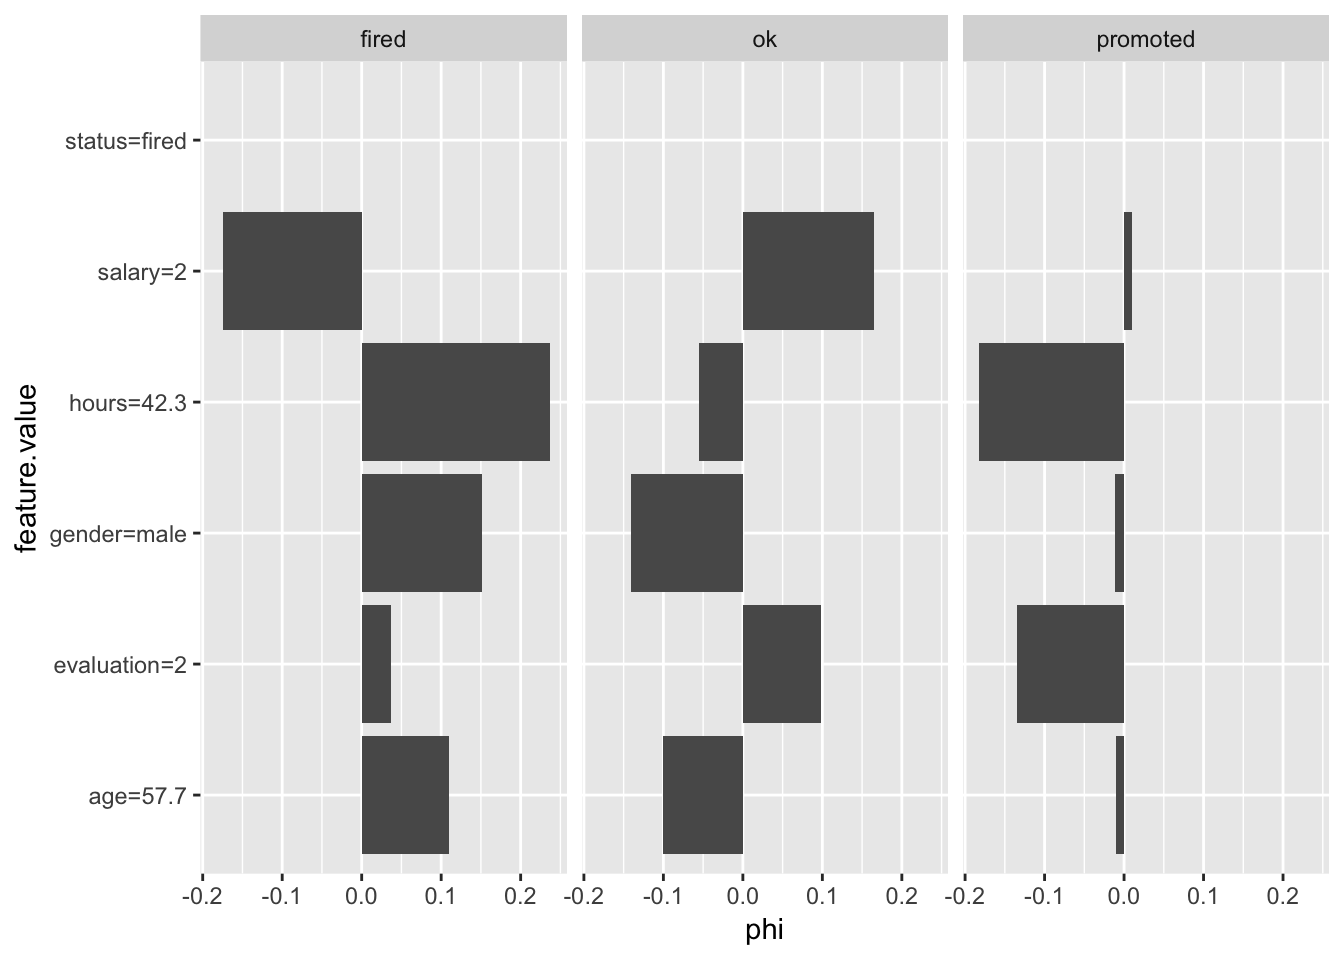
\includegraphics{PM_VEE_files/figure-latex/unnamed-chunk-56-1.pdf}

\hypertarget{shapley}{%
\section{Average variable attributions}\label{shapley}}

In the Section \ref{modelAgnosticAttribution} we show the problem
related to the ordering of variables. In the Section \ref{breakDown} we
show an approach in which the ordering was determined based on single
step assessment of variable importance.

In this section we introduce other, very popular approach for additive
variable attribution. The problem of contributions that depends on the
variable ordering is solved by averaging over all possible orderings.

This method is motivated with results in cooperative game theory and was
first introduced in \citep{Strumbelj2014}. Wide adoption of this method
comes with a NIPS 2017 paper \citep{SHAP} and python library SHAP
\texttt{https://github.com/slundberg/shap}. Authors of the SHAP method
introduced also efficient algorithm for tree-based models, see
\citep{TreeSHAP}.

\hypertarget{intuition-7}{%
\subsection{Intuition}\label{intuition-7}}

Since in sequential attribution effect depends on the ordering. Here the
idea is to average across all possible orderings.

TODO: a nice example

\hypertarget{method-7}{%
\subsection{Method}\label{method-7}}

The name \emph{Shapley Values} comes from the solution in cooperative
game theory attributed to Lloyd Shapley. The original problem was to
assess how important is each player to the overall cooperation, and what
payoff can he or she reasonably expect from the coalition?
\citep{shapleybook1952}

In the context of model interpretability the payoff is the average model
response while the players are the variables in the conditioning. Then
Formula for variable contributions is following.

\[
v(f, x^*, i) = \frac 1{|P|}\sum_{S \subseteq P\setminus \{i\}}  {{|P|-1}\choose{|S|}}^{-1} \left(E [f(X) | X_{S \cup \{i\}} = x^*_{S \cup \{i\}}] - E [f(X) | X_{S} = x^*_{S}]\right)
\] where \(P = \{1, \ldots, p\}\) is the set of all variables. The
intuition beyond this contribution is following. We consider all
possible orderings of variables (yes, there is \(2^p\) of them) and
calculate the contribution of variable \(i\) as an average from
contributions calculated in particular orderings.

The part
\(E[f(X) | X_{S \cup \{i\}} = x^*_{S \cup \{i\}}] - E [f(X) | X_{S} = x^*_{S}]\)
is the contribution of variable \(i\) which is introduces after
variables from \(S\).

Time complexity of this method is \(O(2^p)\) where \(p\) stands for the
number of variables. Such complexity makes this method impractical for
most cases. Fortunately it is enough to assess this value.
\citep{Strumbelj2014} proposed to use sampling. \citep{TreeSHAP}
proposed fast implementations for tree based ensembles.

\textbf{Properties}

Shaply values have (as a single unique solution) following properties

\begin{itemize}
\tightlist
\item
  Local accuracy. Sum of attributions is equal to the model response. \[
  f(x^*) = \sum_{i}   v(f, x^*, i) 
  \]
\item
  Missingness, if simplified (add to notation) input is 0, then it's
  impact is also 0 \[
  x_i^* = 0 implies   v(f, x^*, i) = 0
  \]
\item
  Consistency, if a new model \(g\) is larger for model \(f\) then it's
  attributions are larger than attributions for \(f\).
\end{itemize}

\hypertarget{example-hire-or-fire-2}{%
\subsection{Example: Hire or Fire?}\label{example-hire-or-fire-2}}

\hypertarget{pros-and-cons-7}{%
\subsection{Pros and cons}\label{pros-and-cons-7}}

Shapley Values give a uniform approach to decompose model prediction
into parts that can be attributed additively to variables. Below we
summarize key strengths and weaknesses of this approach.

\textbf{Pros}

\begin{itemize}
\tightlist
\item
  There is a nice theory based on cooperative games.
\item
  \citep{SHAP} shows that this method unifies different approaches to
  additive features attribution, like DeepLIFT, Layer-Wise Relevance
  Propagation, LIME.
\item
  There is efficient implementation available for Python.
\item
  \citep{SHAP} shows more desired properties of this method, like
  symmetry or additivity.
\end{itemize}

\textbf{Cons}

\begin{itemize}
\tightlist
\item
  The exact calculation of Shapley values is time consuming.
\item
  If the model is not additive, then the Shaply scores may be
  misleading. And there is no way to determine if model is far from
  additiveness.
\end{itemize}

Note that fully additive model solutions presented in sections
\ref{modelAgnosticAttribution}, \ref{breakDown} and \ref{shapley} lead
to same variable contributions.

\hypertarget{code-snippets-for-r-6}{%
\subsection{Code snippets for R}\label{code-snippets-for-r-6}}

In this section we will present an example based on the \texttt{HR}
dataset and Random Forest model \citep{R-randomForest}. See the Section
\ref{HRdataset} for more details.

\begin{Shaded}
\begin{Highlighting}[]
\KeywordTok{library}\NormalTok{(}\StringTok{"DALEX"}\NormalTok{)}
\KeywordTok{library}\NormalTok{(}\StringTok{"randomForest"}\NormalTok{)}
\KeywordTok{set.seed}\NormalTok{(}\DecValTok{123}\NormalTok{)}
\NormalTok{model_rf <-}\StringTok{ }\KeywordTok{randomForest}\NormalTok{(status }\OperatorTok{~}\StringTok{ }\NormalTok{gender }\OperatorTok{+}\StringTok{ }\NormalTok{age }\OperatorTok{+}\StringTok{ }\NormalTok{hours }\OperatorTok{+}\StringTok{ }\NormalTok{evaluation }\OperatorTok{+}\StringTok{ }\NormalTok{salary, }\DataTypeTok{data =}\NormalTok{ HR)}
\end{Highlighting}
\end{Shaded}

First, we use a \texttt{shapper} package - a wrapper over SHAP python
package.

\begin{Shaded}
\begin{Highlighting}[]
\KeywordTok{library}\NormalTok{(}\StringTok{"shapper"}\NormalTok{)}
\NormalTok{Y_train <-}\StringTok{ }\NormalTok{HR}\OperatorTok{$}\NormalTok{status}
\NormalTok{x_train <-}\StringTok{ }\NormalTok{HR[ , }\DecValTok{-6}\NormalTok{]}
\NormalTok{x_train}\OperatorTok{$}\NormalTok{gender <-}\StringTok{ }\KeywordTok{as.numeric}\NormalTok{(x_train}\OperatorTok{$}\NormalTok{gender)}
\NormalTok{model_rfs <-}\StringTok{ }\KeywordTok{randomForest}\NormalTok{(}\DataTypeTok{x =}\NormalTok{ x_train, }\DataTypeTok{y =}\NormalTok{ Y_train)}

\NormalTok{p_fun <-}\StringTok{ }\ControlFlowTok{function}\NormalTok{(x, data)\{}
  \KeywordTok{predict}\NormalTok{(x, }\DataTypeTok{newdata =}\NormalTok{ data, }\DataTypeTok{type =} \StringTok{"prob"}\NormalTok{)}
\NormalTok{\}}

\NormalTok{new_observation <-}\StringTok{ }\KeywordTok{data.frame}\NormalTok{(}\DataTypeTok{gender =} \DecValTok{1}\NormalTok{,}
                      \DataTypeTok{age =} \FloatTok{57.7}\NormalTok{,}
                      \DataTypeTok{hours =} \FloatTok{42.3}\NormalTok{,}
                      \DataTypeTok{evaluation =} \DecValTok{2}\NormalTok{,}
                      \DataTypeTok{salary =} \DecValTok{2}\NormalTok{)}

\NormalTok{x <-}\StringTok{ }\KeywordTok{individual_variable_effect}\NormalTok{(}\DataTypeTok{x =}\NormalTok{ model_rfs, }\DataTypeTok{data =}\NormalTok{ x_train, }\DataTypeTok{predict_function =}\NormalTok{ p_fun,}
                               \DataTypeTok{new_observation =}\NormalTok{ new_observation)}

\CommentTok{#plot(x)}
\KeywordTok{library}\NormalTok{(}\StringTok{"ggplot2"}\NormalTok{)}

\NormalTok{x}\OperatorTok{$}\StringTok{`}\DataTypeTok{_vname_}\StringTok{`}\NormalTok{ <-}\StringTok{ }\KeywordTok{reorder}\NormalTok{(x}\OperatorTok{$}\StringTok{`}\DataTypeTok{_vname_}\StringTok{`}\NormalTok{, x}\OperatorTok{$}\StringTok{`}\DataTypeTok{_attribution_}\StringTok{`}\NormalTok{, }\ControlFlowTok{function}\NormalTok{(z) }\OperatorTok{-}\KeywordTok{sum}\NormalTok{(}\KeywordTok{abs}\NormalTok{(z)))}
\KeywordTok{levels}\NormalTok{(x}\OperatorTok{$}\StringTok{`}\DataTypeTok{_vname_}\StringTok{`}\NormalTok{) <-}\StringTok{ }\KeywordTok{paste}\NormalTok{(}\KeywordTok{sapply}\NormalTok{(}\DecValTok{1}\OperatorTok{:}\DecValTok{6}\NormalTok{, substr, }\DataTypeTok{x=}\StringTok{"        "}\NormalTok{, }\DataTypeTok{start=}\DecValTok{1}\NormalTok{), }\KeywordTok{levels}\NormalTok{(x}\OperatorTok{$}\StringTok{`}\DataTypeTok{_vname_}\StringTok{`}\NormalTok{))}

\KeywordTok{ggplot}\NormalTok{(x, }\KeywordTok{aes}\NormalTok{(}\DataTypeTok{x=}\StringTok{`}\DataTypeTok{_vname_}\StringTok{`}\NormalTok{, }\DataTypeTok{xend=}\StringTok{`}\DataTypeTok{_vname_}\StringTok{`}\NormalTok{, }
              \DataTypeTok{yend =} \StringTok{`}\DataTypeTok{_yhat_mean_}\StringTok{`}\NormalTok{, }\DataTypeTok{y =} \StringTok{`}\DataTypeTok{_yhat_mean_}\StringTok{`} \OperatorTok{+}\StringTok{ `}\DataTypeTok{_attribution_}\StringTok{`}\NormalTok{, }
              \DataTypeTok{color=}\StringTok{`}\DataTypeTok{_sign_}\StringTok{`}\NormalTok{)) }\OperatorTok{+}
\StringTok{  }\KeywordTok{geom_segment}\NormalTok{(}\DataTypeTok{arrow =} \KeywordTok{arrow}\NormalTok{(}\DataTypeTok{length=}\KeywordTok{unit}\NormalTok{(}\FloatTok{0.30}\NormalTok{,}\StringTok{"cm"}\NormalTok{), }\DataTypeTok{ends=}\StringTok{"first"}\NormalTok{, }\DataTypeTok{type =} \StringTok{"closed"}\NormalTok{)) }\OperatorTok{+}\StringTok{ }
\StringTok{  }\KeywordTok{geom_text}\NormalTok{(}\KeywordTok{aes}\NormalTok{(}\DataTypeTok{label =} \KeywordTok{round}\NormalTok{(}\StringTok{`}\DataTypeTok{_attribution_}\StringTok{`}\NormalTok{, }\DecValTok{2}\NormalTok{)), }\DataTypeTok{nudge_x =} \FloatTok{0.45}\NormalTok{) }\OperatorTok{+}
\StringTok{  }\KeywordTok{geom_segment}\NormalTok{(}\KeywordTok{aes}\NormalTok{(}\DataTypeTok{x =} \StringTok{"_predicted_"}\NormalTok{,}\DataTypeTok{xend =} \StringTok{"_predicted_"}\NormalTok{,}
                   \DataTypeTok{y =} \StringTok{`}\DataTypeTok{_yhat_}\StringTok{`}\NormalTok{, }\DataTypeTok{yend =} \StringTok{`}\DataTypeTok{_yhat_mean_}\StringTok{`}\NormalTok{), }\DataTypeTok{size =} \DecValTok{2}\NormalTok{, }\DataTypeTok{color=}\StringTok{"black"}\NormalTok{,}
               \DataTypeTok{arrow =} \KeywordTok{arrow}\NormalTok{(}\DataTypeTok{length=}\KeywordTok{unit}\NormalTok{(}\FloatTok{0.30}\NormalTok{,}\StringTok{"cm"}\NormalTok{), }\DataTypeTok{ends=}\StringTok{"first"}\NormalTok{, }\DataTypeTok{type =} \StringTok{"closed"}\NormalTok{)) }\OperatorTok{+}\StringTok{ }
\StringTok{  }\KeywordTok{geom_text}\NormalTok{(}\KeywordTok{aes}\NormalTok{(}\DataTypeTok{x =} \StringTok{"_predicted_"}\NormalTok{, }
                \DataTypeTok{y =} \StringTok{`}\DataTypeTok{_yhat_}\StringTok{`}\NormalTok{, }\DataTypeTok{label =} \KeywordTok{round}\NormalTok{(}\StringTok{`}\DataTypeTok{_yhat_}\StringTok{`}\NormalTok{, }\DecValTok{2}\NormalTok{)), }\DataTypeTok{nudge_x =} \FloatTok{0.45}\NormalTok{, }\DataTypeTok{color=}\StringTok{"black"}\NormalTok{) }\OperatorTok{+}
\StringTok{  }\KeywordTok{geom_hline}\NormalTok{(}\KeywordTok{aes}\NormalTok{(}\DataTypeTok{yintercept =} \StringTok{`}\DataTypeTok{_yhat_mean_}\StringTok{`}\NormalTok{)) }\OperatorTok{+}\StringTok{ }
\StringTok{  }\KeywordTok{facet_grid}\NormalTok{(}\StringTok{`}\DataTypeTok{_label_}\StringTok{`}\OperatorTok{~}\StringTok{`}\DataTypeTok{_ylevel_}\StringTok{`}\NormalTok{) }\OperatorTok{+}
\StringTok{  }\KeywordTok{scale_color_manual}\NormalTok{(}\DataTypeTok{values =}  \KeywordTok{c}\NormalTok{(}\StringTok{`}\DataTypeTok{-}\StringTok{`}\NormalTok{ =}\StringTok{ "#d8b365"}\NormalTok{, }\StringTok{`}\DataTypeTok{0}\StringTok{`}\NormalTok{ =}\StringTok{ "#f5f5f5"}\NormalTok{, }\StringTok{`}\DataTypeTok{+}\StringTok{`}\NormalTok{ =}\StringTok{ "#5ab4ac"}\NormalTok{, }
                                \DataTypeTok{X =} \StringTok{"darkgrey"}\NormalTok{)) }\OperatorTok{+}
\StringTok{  }\KeywordTok{coord_flip}\NormalTok{() }\OperatorTok{+}\StringTok{ }\KeywordTok{theme_minimal}\NormalTok{() }\OperatorTok{+}\StringTok{ }\KeywordTok{theme}\NormalTok{(}\DataTypeTok{legend.position=}\StringTok{"none"}\NormalTok{) }\OperatorTok{+}\StringTok{ }\KeywordTok{xlab}\NormalTok{(}\StringTok{""}\NormalTok{) }\OperatorTok{+}\StringTok{ }\KeywordTok{ylab}\NormalTok{(}\StringTok{""}\NormalTok{)}
\end{Highlighting}
\end{Shaded}

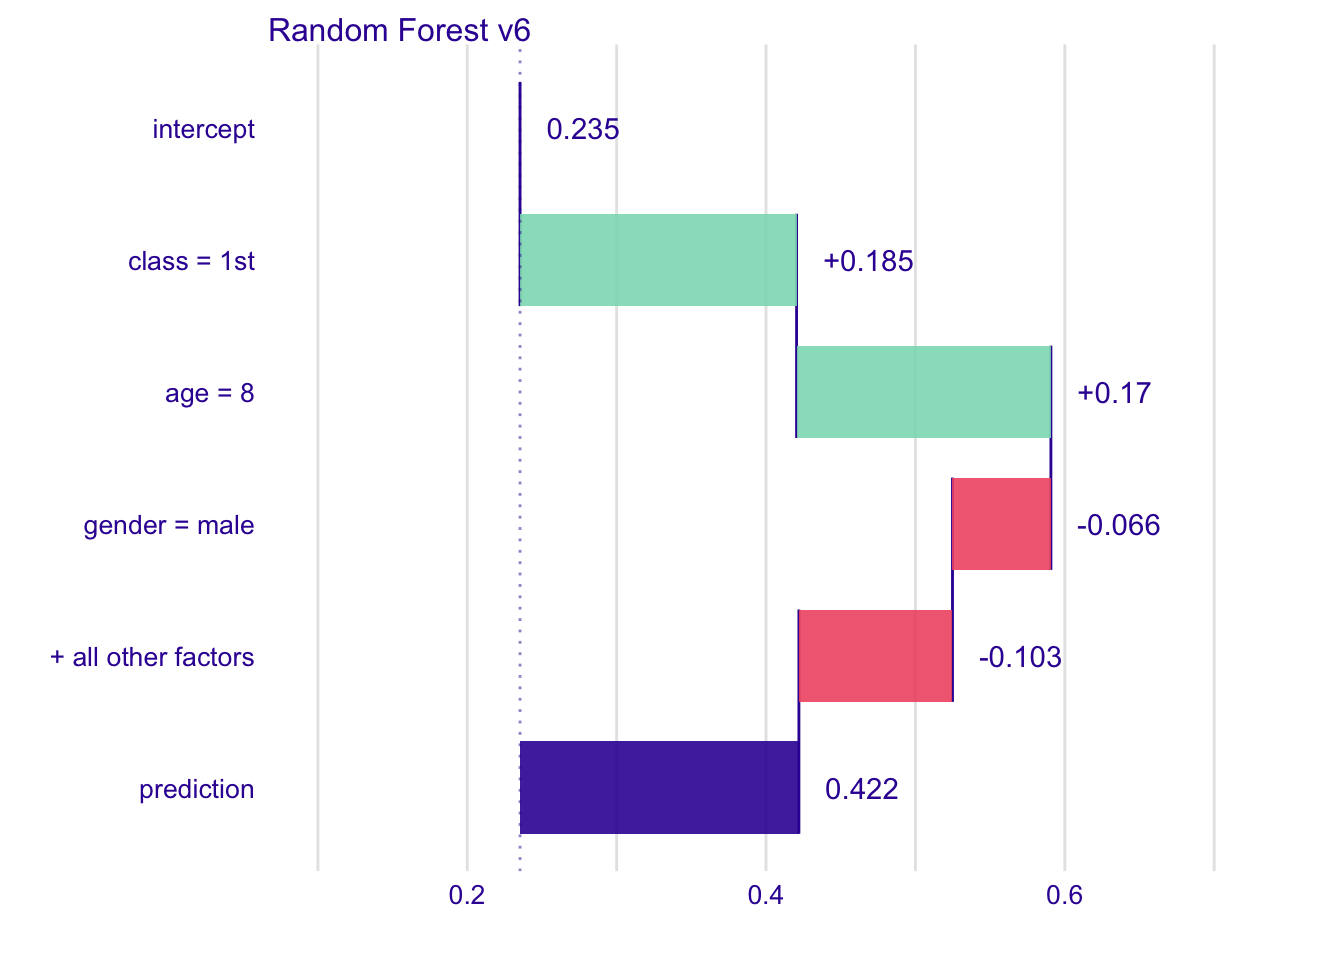
\includegraphics{PM_VEE_files/figure-latex/unnamed-chunk-58-1.pdf}

Here we use the \texttt{iml} package, see more examples in
\citep{imlPackage}.

\begin{Shaded}
\begin{Highlighting}[]
\KeywordTok{library}\NormalTok{(}\StringTok{"iml"}\NormalTok{)}
\NormalTok{explainer_rf =}\StringTok{ }\NormalTok{Predictor}\OperatorTok{$}\KeywordTok{new}\NormalTok{(model_rf, }\DataTypeTok{data =}\NormalTok{ HR, }\DataTypeTok{type=}\StringTok{"prob"}\NormalTok{)}
\end{Highlighting}
\end{Shaded}

Explanations for a new observation.

\begin{Shaded}
\begin{Highlighting}[]
\NormalTok{new_observation <-}\StringTok{ }\KeywordTok{data.frame}\NormalTok{(}\DataTypeTok{gender =} \KeywordTok{factor}\NormalTok{(}\StringTok{"male"}\NormalTok{, }\DataTypeTok{levels =} \KeywordTok{c}\NormalTok{(}\StringTok{"male"}\NormalTok{, }\StringTok{"female"}\NormalTok{)),}
                      \DataTypeTok{age =} \FloatTok{57.7}\NormalTok{,}
                      \DataTypeTok{hours =} \FloatTok{42.3}\NormalTok{,}
                      \DataTypeTok{evaluation =} \DecValTok{2}\NormalTok{,}
                      \DataTypeTok{salary =} \DecValTok{2}\NormalTok{,}
                      \DataTypeTok{status =} \KeywordTok{factor}\NormalTok{(}\StringTok{"fired"}\NormalTok{))}

\NormalTok{shapley =}\StringTok{ }\NormalTok{Shapley}\OperatorTok{$}\KeywordTok{new}\NormalTok{(explainer_rf, }\DataTypeTok{x.interest =}\NormalTok{ new_observation)}
\NormalTok{shapley}
\end{Highlighting}
\end{Shaded}

And the plot with Shapley attributions.

\begin{Shaded}
\begin{Highlighting}[]
\KeywordTok{plot}\NormalTok{(shapley)}
\end{Highlighting}
\end{Shaded}

See more examples for \texttt{iml} package in the \citep{molnar} book.

\hypertarget{LIME}{%
\section{Local approximations with white-box model}\label{LIME}}

A different approach to explanations of a single observations is through
surrogate models. Models that easy to understand and are similar to
black box model around the point of interest.

Variable attribution methods, that were presented in the Section
\ref{breakDown} are not interested in the local curvature of the model.
They rather compare model prediction against average model prediction
and they use probability structure of the dataset.

The complementary approach would be to directly explore information
about model curvature around point of interest. In the section
\ref{ceterisParibus} we introduced Ceteris Paribus tool for such what-if
analysis. But the limitation of ceteris Paribus pltos is that they
explore changes along single dimension or pairs of dimensions.

In this section we describe an another approach based on local
approximations with white-box models. This approach will also
investigate local curvature of the model but indirectly, through
surrogate white-box models.

The most known method from this class if LIME (Local Interpretable
Model-Agnostic Explanations), introduced in the paper \emph{Why Should I
Trust You?: Explaining the Predictions of Any Classifier} \citep{lime}.
This methods and it's clones are now implemented in various R and python
packages, see for example \citep{R-lime}, \citep{R-live} or
\citep{R-iml}.

\hypertarget{intuition-8}{%
\subsection{Intuition}\label{intuition-8}}

\hypertarget{method-8}{%
\subsection{Method}\label{method-8}}

The LIME method, and its clones, has following properties:

\begin{itemize}
\tightlist
\item
  \emph{model-agnostic}, they do not imply any assumptions on model
  structure,
\item
  \emph{interpretable representation}, model input is transformed into a
  feature space that is easier to understand. One of applications comes
  from image data, single pixels are not easy to interpret, thus the
  LIME method decompose image into a series of super pixels, that are
  easier to interpret to humans,
\item
  \emph{local fidelity} means that the explanations shall be locally
  well fitted to the black-box model.
\end{itemize}

Therefore the objective is to find a local model \(M^L\) that
approximates the black box model \(f\) in the point \(x^*\). As a
solution the penalized loss function is used. The white-box model that
is used for explanations satisfies following condition.

\[
M^*(x^*) = \arg \min_{g \in G} L(f, g, \Pi_{x^*}) + \Omega (g) 
\] where \(G\) is a family of white box models (e.g.~linear models),
\(\Pi_{x^*}\) is neighbourhood of \(x^*\) and \(\Omega\) stands for
model complexity.

\begin{figure}

{\centering 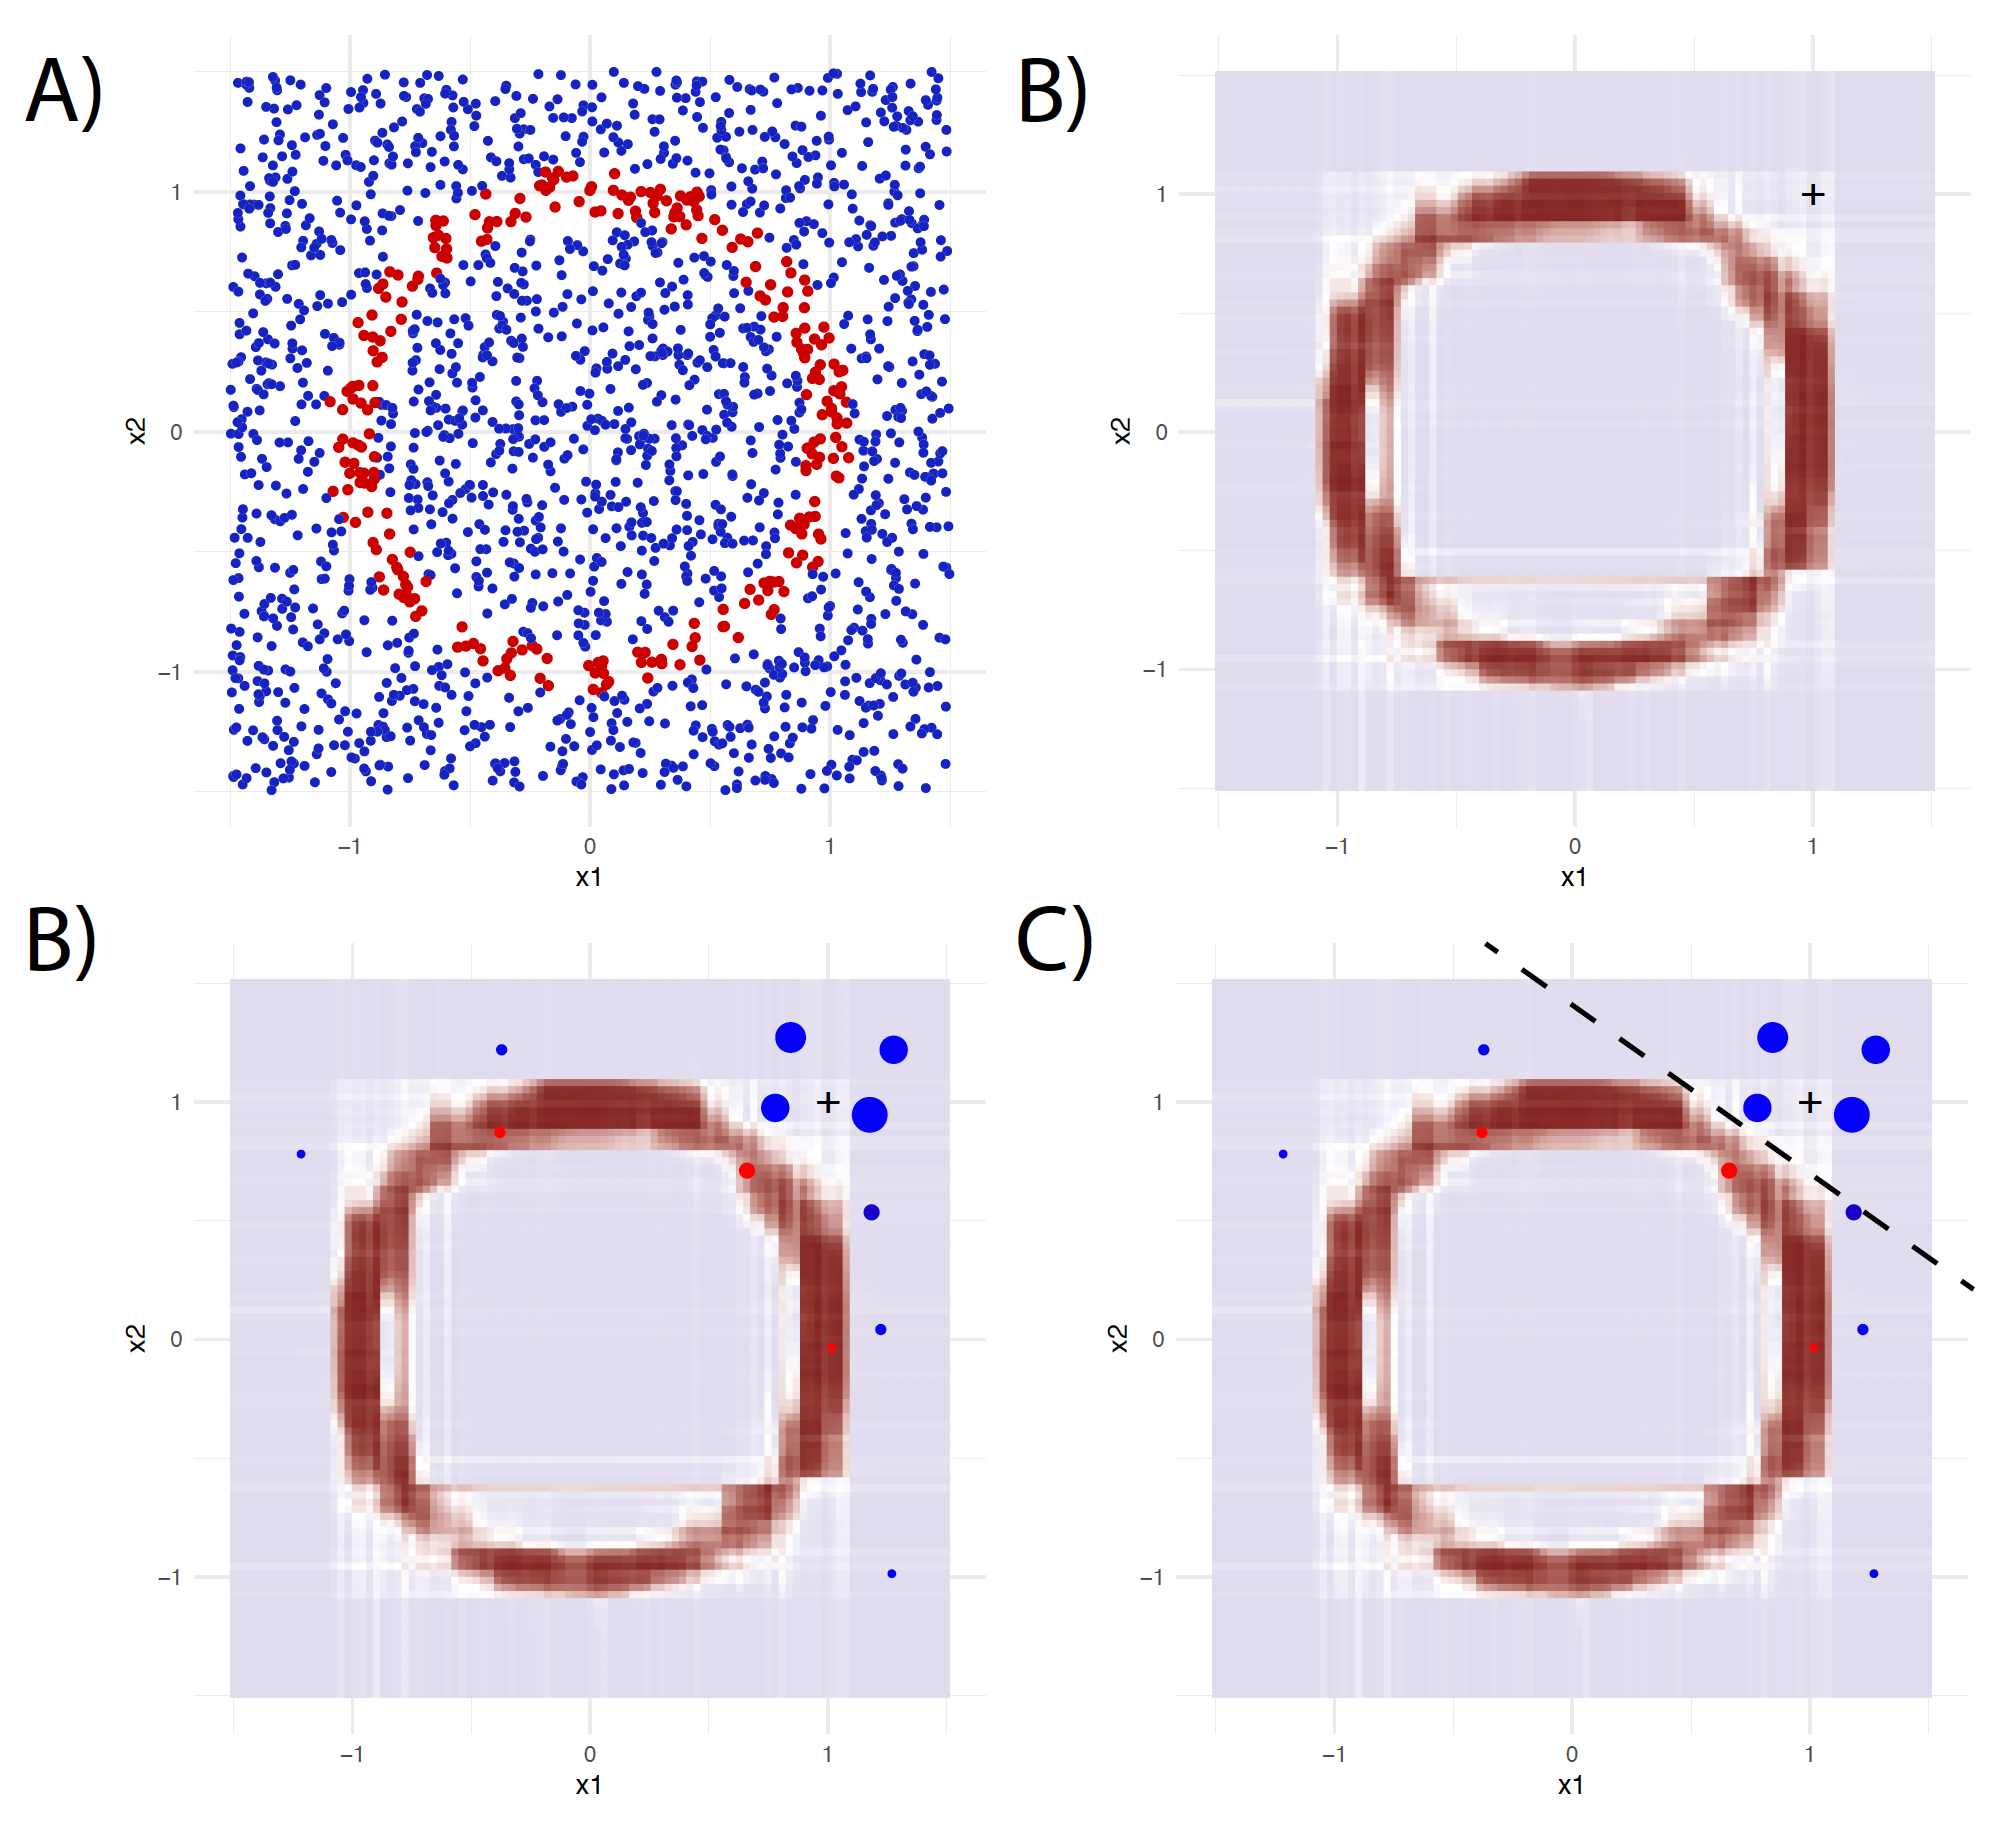
\includegraphics[width=0.7\linewidth]{figure/circle_4panels} 

}

\caption{(fig:LIME1) A schematic idea behind local model approximations. Panel A shows training data, colors correspond to classess. Panel B showhs results fom the Random Forest model, whis is where the algorithm starts. Panel C shows new data sampled around the point of interest. Their color correspond to model response. Panel D shows fitted linear model that approximated the random forest model around point of interest}\label{fig:LIME1}
\end{figure}

The algorithm is composed from three steps:

\begin{itemize}
\tightlist
\item
  Identification of interpretable data representations,
\item
  Local sampling around the point of interest,
\item
  Fitting a white box model in this neighbouhood
\end{itemize}

\textbf{Identification of interpretable data representations}

For image data, single pixel is not an interpretable feature. In this
step the input space of the model is transformed to input space that is
easier to understand for human. The image may be decomposed into parts
and represented as presence/absence of some part of an image.

\textbf{Local sampling around the point of interest}

Once the interpretable data representation is identified, then the
neighbourhood around point of interest needs to be explored.

\textbf{Fitting a white box model in this neighbouhood}

Any model that is easy to interpret may be fitted to this data, like
decision tree or rule based system. However in practice the most common
family of models are linear models.

\hypertarget{example-hire-or-fire-3}{%
\subsection{Example: Hire or Fire?}\label{example-hire-or-fire-3}}

\hypertarget{pros-and-cons-8}{%
\subsection{Pros and cons}\label{pros-and-cons-8}}

Local approximations are model agnostic, can be applied to any
predictive model. Below we summarize key strengths and weaknesses of
this approach.

\textbf{Pros}

\begin{itemize}
\tightlist
\item
  This method is highly adopted in text analysis and image analysis, in
  part thanks to the interpretable data representations.
\item
  The intuition behind the model is straightforward
\item
  Model explanations are sparse, thus only small number of features is
  used
\end{itemize}

\textbf{Cons}

\begin{itemize}
\tightlist
\item
  For continuous variables and tabular data it is not that easy to find
  interpretable representations
\item
  The black-box model approximated the data and the white box model
  approximates the black box model. We do not have control over the
  quality of local fit of the white box model, thus the surrogate model
  may be misleading.
\item
  Due to the \emph{curse of dimensionality}, for high dimensional space
  points are sparse.
\end{itemize}

\hypertarget{code-snippets-for-r-7}{%
\subsection{Code snippets for R}\label{code-snippets-for-r-7}}

In this section we present example application of \texttt{lime}
\citep{R-lime} and \texttt{live} \citep{R-live} packages. Note that this
method is also implemented in \texttt{iml} \citep{R-iml} and other
packages. These pacakages differ in some details and also results in
different explanations.

\textbf{Model preparation}

In this section we will present examples based on the \texttt{HR}
dataset. See the Section \ref{HRdataset} for more details.

\begin{Shaded}
\begin{Highlighting}[]
\KeywordTok{library}\NormalTok{(}\StringTok{"DALEX"}\NormalTok{)}
\KeywordTok{head}\NormalTok{(HR)}
\end{Highlighting}
\end{Shaded}

\begin{verbatim}
##   gender      age    hours evaluation salary   status
## 1   male 32.58267 41.88626          3      1    fired
## 2 female 41.21104 36.34339          2      5    fired
## 3   male 37.70516 36.81718          3      0    fired
## 4 female 30.06051 38.96032          3      2    fired
## 5   male 21.10283 62.15464          5      3 promoted
## 6   male 40.11812 69.53973          2      0    fired
\end{verbatim}

The problem here is to predict average price for square meter for an
apartment. Let's build a random forest model with \texttt{randomForest}
package \citep{R-randomForest}.

\begin{Shaded}
\begin{Highlighting}[]
\KeywordTok{library}\NormalTok{(}\StringTok{"randomForest"}\NormalTok{)}
\NormalTok{rf_model <-}\StringTok{ }\KeywordTok{randomForest}\NormalTok{(status }\OperatorTok{~}\StringTok{ }\NormalTok{gender }\OperatorTok{+}\StringTok{ }\NormalTok{age }\OperatorTok{+}\StringTok{ }\NormalTok{hours }\OperatorTok{+}\StringTok{ }\NormalTok{evaluation }\OperatorTok{+}\StringTok{ }\NormalTok{salary, }\DataTypeTok{data =}\NormalTok{ HR)}
\NormalTok{rf_model}
\end{Highlighting}
\end{Shaded}

\begin{verbatim}
## 
## Call:
##  randomForest(formula = status ~ gender + age + hours + evaluation +      salary, data = HR) 
##                Type of random forest: classification
##                      Number of trees: 500
## No. of variables tried at each split: 2
## 
##         OOB estimate of  error rate: 27.49%
## Confusion matrix:
##          fired   ok promoted class.error
## fired     2270  384      201   0.2049037
## ok         528 1244      449   0.4398919
## promoted   206  389     2176   0.2147239
\end{verbatim}

\begin{Shaded}
\begin{Highlighting}[]
\NormalTok{new_observation <-}\StringTok{ }\KeywordTok{data.frame}\NormalTok{(}\DataTypeTok{gender =} \KeywordTok{factor}\NormalTok{(}\StringTok{"male"}\NormalTok{, }\DataTypeTok{levels =} \KeywordTok{c}\NormalTok{(}\StringTok{"male"}\NormalTok{, }\StringTok{"female"}\NormalTok{)),}
                      \DataTypeTok{age =} \FloatTok{57.7}\NormalTok{,}
                      \DataTypeTok{hours =} \FloatTok{42.3}\NormalTok{,}
                      \DataTypeTok{evaluation =} \DecValTok{2}\NormalTok{,}
                      \DataTypeTok{salary =} \DecValTok{2}\NormalTok{)}

\KeywordTok{predict}\NormalTok{(rf_model, new_observation, }\DataTypeTok{type =} \StringTok{"prob"}\NormalTok{)}
\end{Highlighting}
\end{Shaded}

\begin{verbatim}
##   fired    ok promoted
## 1 0.784 0.214    0.002
## attr(,"class")
## [1] "matrix" "votes"
\end{verbatim}

\hypertarget{the-lime-pacakge}{%
\subsubsection{\texorpdfstring{\textbf{The lime
pacakge}}{The lime pacakge}}\label{the-lime-pacakge}}

\begin{Shaded}
\begin{Highlighting}[]
\KeywordTok{library}\NormalTok{(}\StringTok{"lime"}\NormalTok{)}
\NormalTok{model_type.randomForest <-}\StringTok{ }\ControlFlowTok{function}\NormalTok{(x, ...) }\StringTok{"classification"}
\NormalTok{lime_rf <-}\StringTok{ }\KeywordTok{lime}\NormalTok{(HR[,}\DecValTok{1}\OperatorTok{:}\DecValTok{5}\NormalTok{], rf_model)}
\NormalTok{explanations <-}\StringTok{ }\NormalTok{lime}\OperatorTok{::}\KeywordTok{explain}\NormalTok{(new_observation[,}\DecValTok{1}\OperatorTok{:}\DecValTok{5}\NormalTok{], lime_rf, }\DataTypeTok{n_labels =} \DecValTok{3}\NormalTok{, }\DataTypeTok{n_features =} \DecValTok{3}\NormalTok{)}
\NormalTok{explanations}
\end{Highlighting}
\end{Shaded}

\begin{verbatim}
##       model_type case    label label_prob  model_r2 model_intercept
## 1 classification    1    fired      0.784 0.1229568       0.2549494
## 2 classification    1    fired      0.784 0.1229568       0.2549494
## 3 classification    1    fired      0.784 0.1229568       0.2549494
## 4 classification    1       ok      0.214 0.1301129       0.1884677
## 5 classification    1       ok      0.214 0.1301129       0.1884677
## 6 classification    1       ok      0.214 0.1301129       0.1884677
## 7 classification    1 promoted      0.002 0.2803287       0.5167543
## 8 classification    1 promoted      0.002 0.2803287       0.5167543
## 9 classification    1 promoted      0.002 0.2803287       0.5167543
##   model_prediction    feature feature_value feature_weight
## 1       0.64320321     gender           2.0    0.018638406
## 2       0.64320321      hours          42.3    0.256064763
## 3       0.64320321 evaluation           2.0    0.113550640
## 4       0.45858087        age          57.7   -0.013851520
## 5       0.45858087 evaluation           2.0    0.205469213
## 6       0.45858087     salary           2.0    0.078495471
## 7       0.00344001        age          57.7   -0.006718524
## 8       0.00344001 evaluation           2.0   -0.317770612
## 9       0.00344001      hours          42.3   -0.188825120
##           feature_desc                      data          prediction
## 1        gender = male 2.0, 57.7, 42.3, 2.0, 2.0 0.784, 0.214, 0.002
## 2 37.6 < hours <= 46.3 2.0, 57.7, 42.3, 2.0, 2.0 0.784, 0.214, 0.002
## 3      evaluation <= 3 2.0, 57.7, 42.3, 2.0, 2.0 0.784, 0.214, 0.002
## 4           50.0 < age 2.0, 57.7, 42.3, 2.0, 2.0 0.784, 0.214, 0.002
## 5      evaluation <= 3 2.0, 57.7, 42.3, 2.0, 2.0 0.784, 0.214, 0.002
## 6      1 < salary <= 2 2.0, 57.7, 42.3, 2.0, 2.0 0.784, 0.214, 0.002
## 7           50.0 < age 2.0, 57.7, 42.3, 2.0, 2.0 0.784, 0.214, 0.002
## 8      evaluation <= 3 2.0, 57.7, 42.3, 2.0, 2.0 0.784, 0.214, 0.002
## 9 37.6 < hours <= 46.3 2.0, 57.7, 42.3, 2.0, 2.0 0.784, 0.214, 0.002
\end{verbatim}

\begin{Shaded}
\begin{Highlighting}[]
\KeywordTok{plot_features}\NormalTok{(explanations)}
\end{Highlighting}
\end{Shaded}

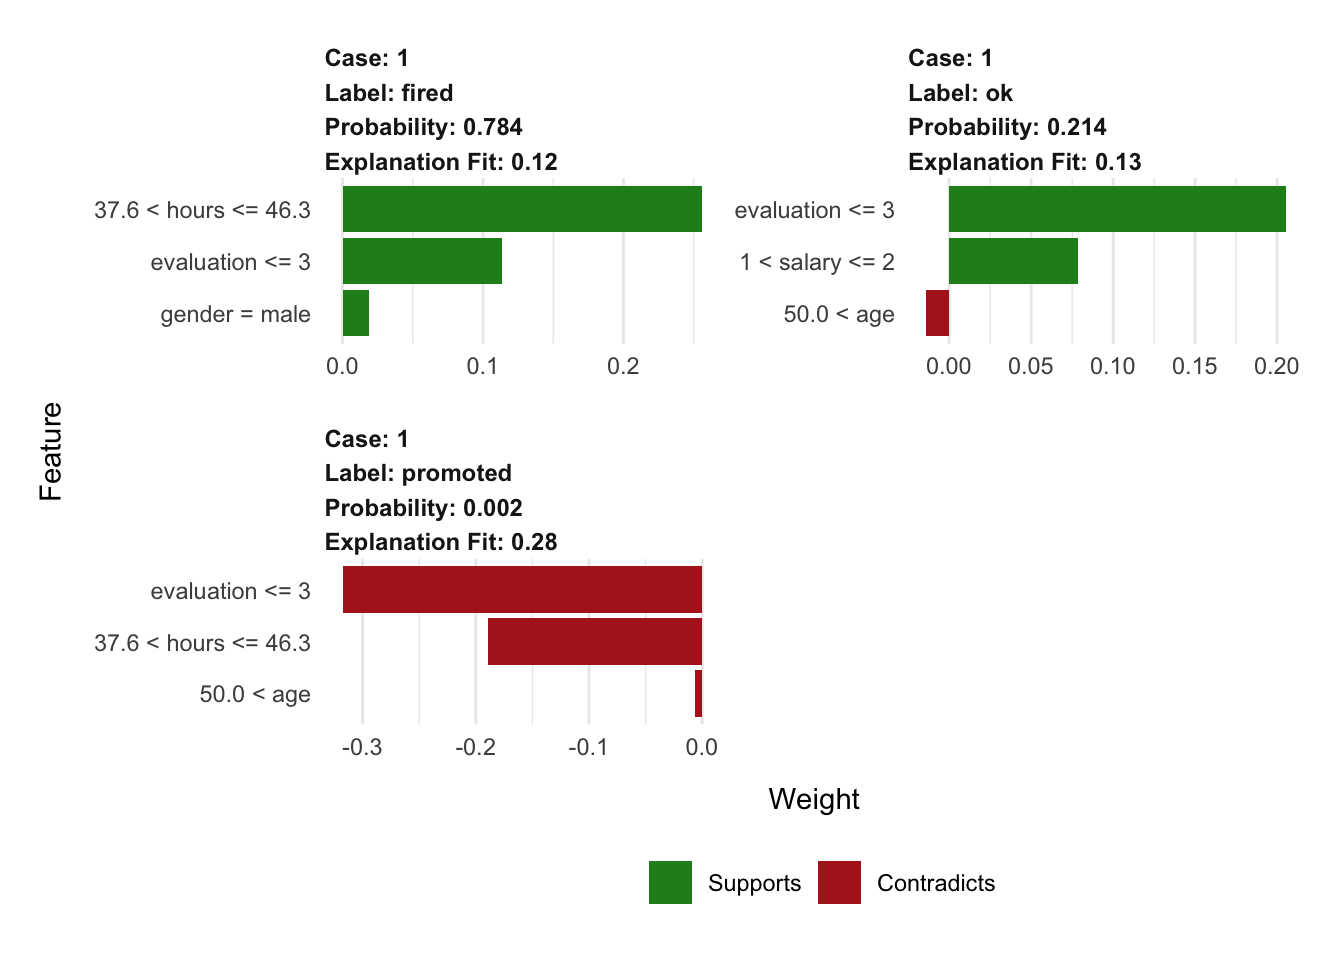
\includegraphics{PM_VEE_files/figure-latex/unnamed-chunk-66-1.pdf}

\hypertarget{the-live-package}{%
\subsubsection{\texorpdfstring{\textbf{The live
package}}{The live package}}\label{the-live-package}}

\begin{Shaded}
\begin{Highlighting}[]
\KeywordTok{library}\NormalTok{(}\StringTok{"live"}\NormalTok{)}

\NormalTok{new_observation}\OperatorTok{$}\NormalTok{status <-}\StringTok{ "fired"}
\NormalTok{explainer_rf_fired <-}\StringTok{ }\KeywordTok{explain}\NormalTok{(rf_model,}
                 \DataTypeTok{data =}\NormalTok{ HR,}
                 \DataTypeTok{y =}\NormalTok{ HR}\OperatorTok{$}\NormalTok{status }\OperatorTok{==}\StringTok{ "fired"}\NormalTok{,}
                 \DataTypeTok{predict_function =} \ControlFlowTok{function}\NormalTok{(m,x) }\KeywordTok{predict}\NormalTok{(m,x, }\DataTypeTok{type =} \StringTok{"prob"}\NormalTok{)[,}\DecValTok{1}\NormalTok{],}
                 \DataTypeTok{label =} \StringTok{"fired"}\NormalTok{)}

\NormalTok{local_model <-}\StringTok{ }\KeywordTok{local_approximation}\NormalTok{(explainer_rf_fired, new_observation, }
                    \DataTypeTok{target_variable_name =} \StringTok{"status"}\NormalTok{, }\DataTypeTok{n_new_obs =} \DecValTok{500}\NormalTok{)}

\NormalTok{local_model}
\end{Highlighting}
\end{Shaded}

\begin{verbatim}
## Dataset: 
##  Observations:  500 
##  Variables:  6 
##  Response variable:  status 
## Explanation model: 
##  Name:  regr.lm 
##  Variable selection wasn't performed 
##  Weights present in the explanation model 
##  R-squared: 0.7596
\end{verbatim}

\begin{Shaded}
\begin{Highlighting}[]
\KeywordTok{plot}\NormalTok{(local_model)}
\end{Highlighting}
\end{Shaded}

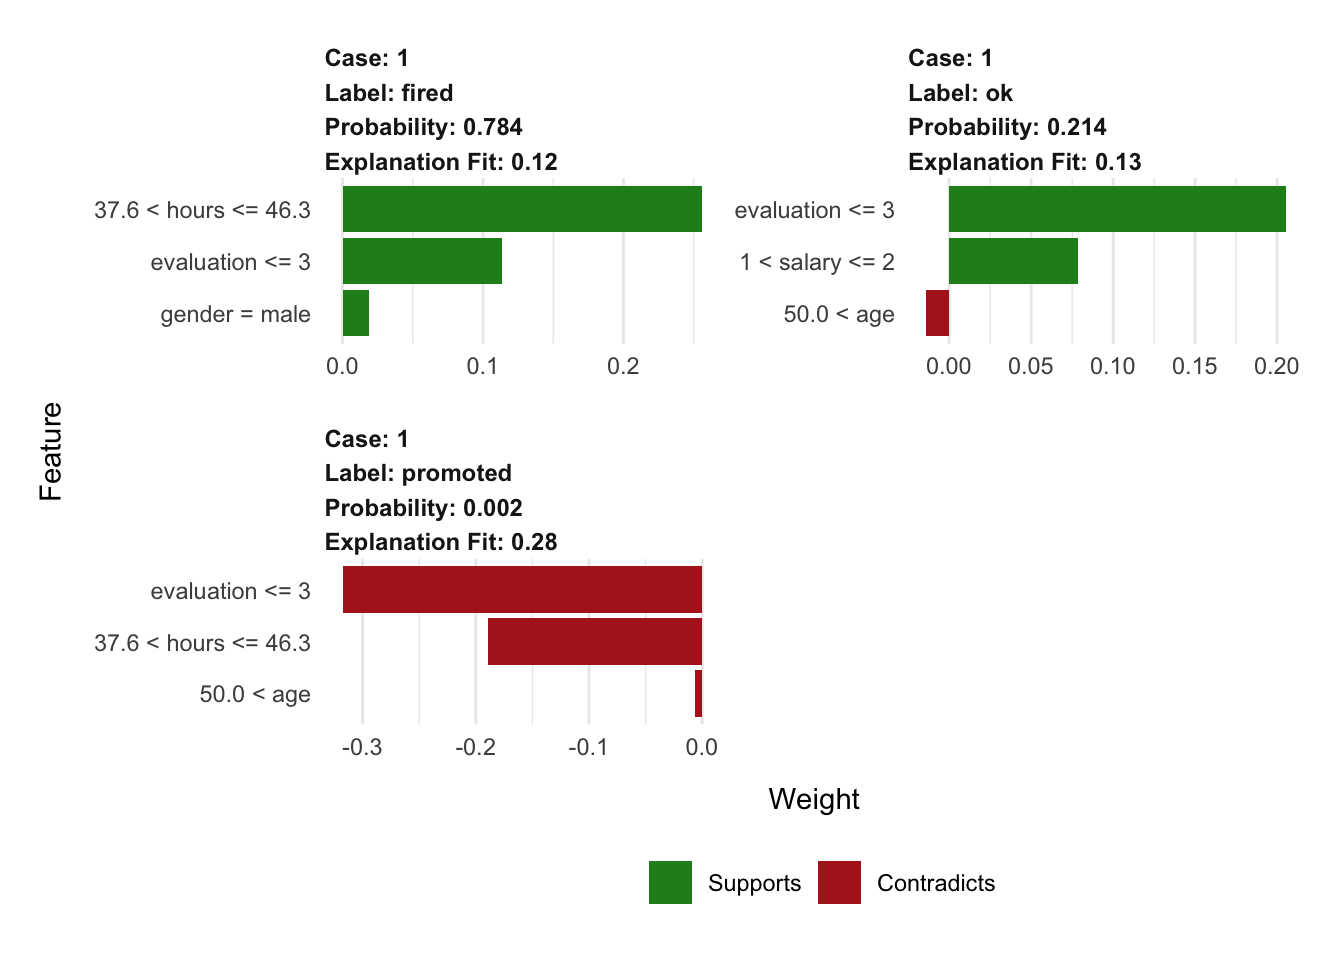
\includegraphics{PM_VEE_files/figure-latex/unnamed-chunk-67-1.pdf}

\begin{Shaded}
\begin{Highlighting}[]
\KeywordTok{plot}\NormalTok{(local_model, }\DataTypeTok{type =} \StringTok{"forest"}\NormalTok{)}
\end{Highlighting}
\end{Shaded}

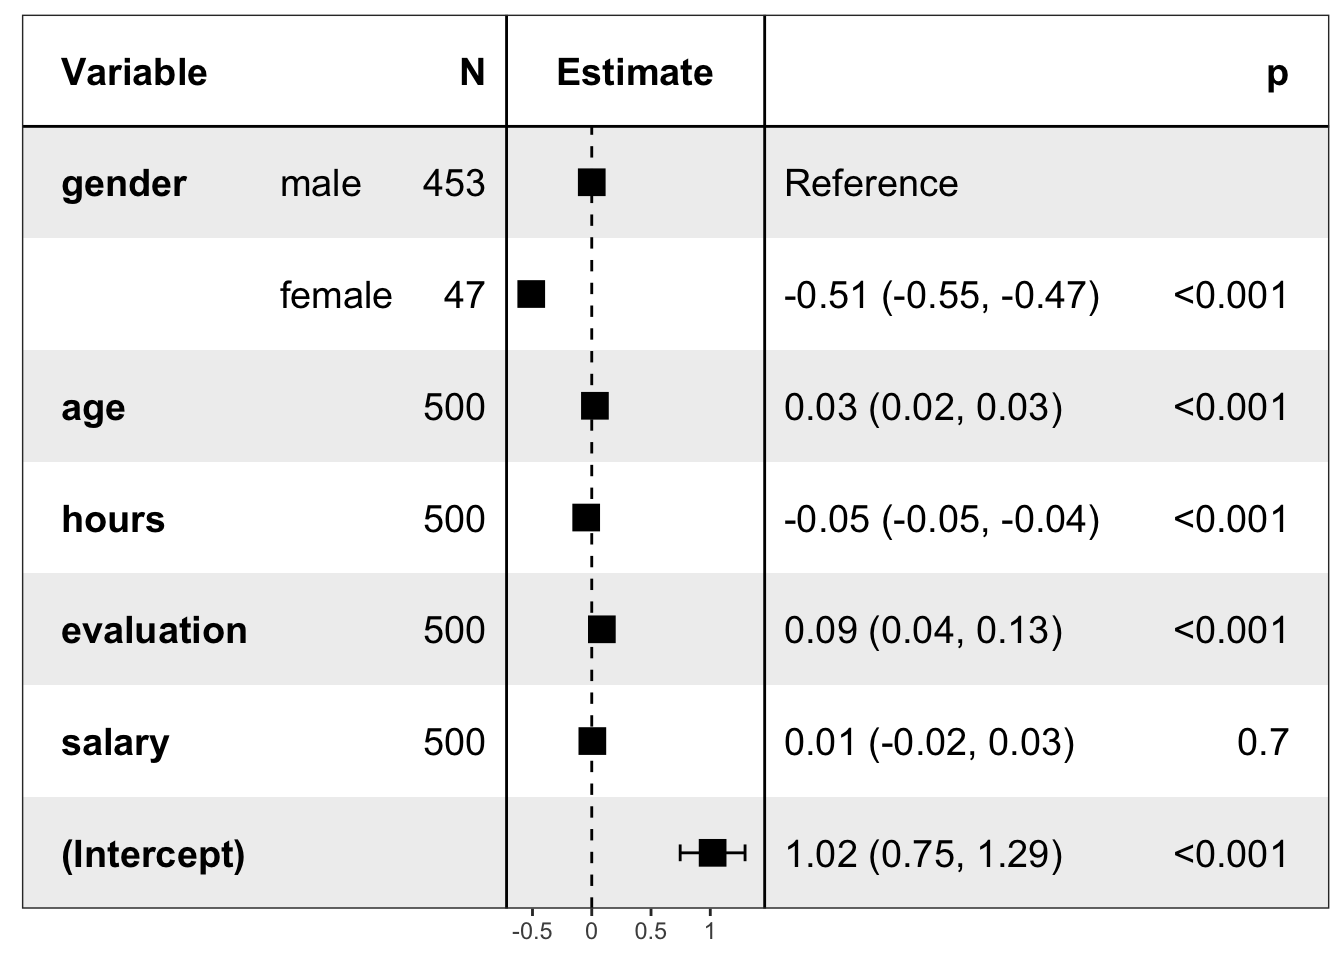
\includegraphics{PM_VEE_files/figure-latex/unnamed-chunk-67-2.pdf}

\hypertarget{the-iml-package}{%
\subsubsection{\texorpdfstring{\textbf{The iml
package}}{The iml package}}\label{the-iml-package}}

\begin{Shaded}
\begin{Highlighting}[]
\KeywordTok{library}\NormalTok{(}\StringTok{"iml"}\NormalTok{)}

\NormalTok{explainer_rf =}\StringTok{ }\NormalTok{Predictor}\OperatorTok{$}\KeywordTok{new}\NormalTok{(rf_model, }\DataTypeTok{data =}\NormalTok{ HR[,}\DecValTok{1}\OperatorTok{:}\DecValTok{5}\NormalTok{])}
\NormalTok{white_box =}\StringTok{ }\NormalTok{LocalModel}\OperatorTok{$}\KeywordTok{new}\NormalTok{(explainer_rf, }\DataTypeTok{x.interest =}\NormalTok{ new_observation[,}\DecValTok{1}\OperatorTok{:}\DecValTok{5}\NormalTok{], }\DataTypeTok{k =} \DecValTok{5}\NormalTok{)}
\NormalTok{white_box}
\end{Highlighting}
\end{Shaded}

\begin{verbatim}
## Interpretation method:  LocalModel 
## 
## 
## Analysed predictor: 
## Prediction task: unknown 
## 
## 
## Analysed data:
## Sampling from data.frame with 7847 rows and 5 columns.
## 
## Head of results:
##           beta x.recoded      effect x.original     feature feature.value
## 1  0.062176640       1.0  0.06217664       male gender=male   gender=male
## 2  0.005789257      57.7  0.33404015       57.7         age      age=57.7
## 3 -0.090772953      42.3 -3.83969593       42.3       hours    hours=42.3
## 4 -0.506977522       2.0 -1.01395504          2  evaluation  evaluation=2
## 5 -0.031598533       2.0 -0.06319707          2      salary      salary=2
## 6 -0.015944921       1.0 -0.01594492       male gender=male   gender=male
##   .class
## 1  fired
## 2  fired
## 3  fired
## 4  fired
## 5  fired
## 6     ok
\end{verbatim}

\begin{Shaded}
\begin{Highlighting}[]
\KeywordTok{plot}\NormalTok{(white_box)}
\end{Highlighting}
\end{Shaded}

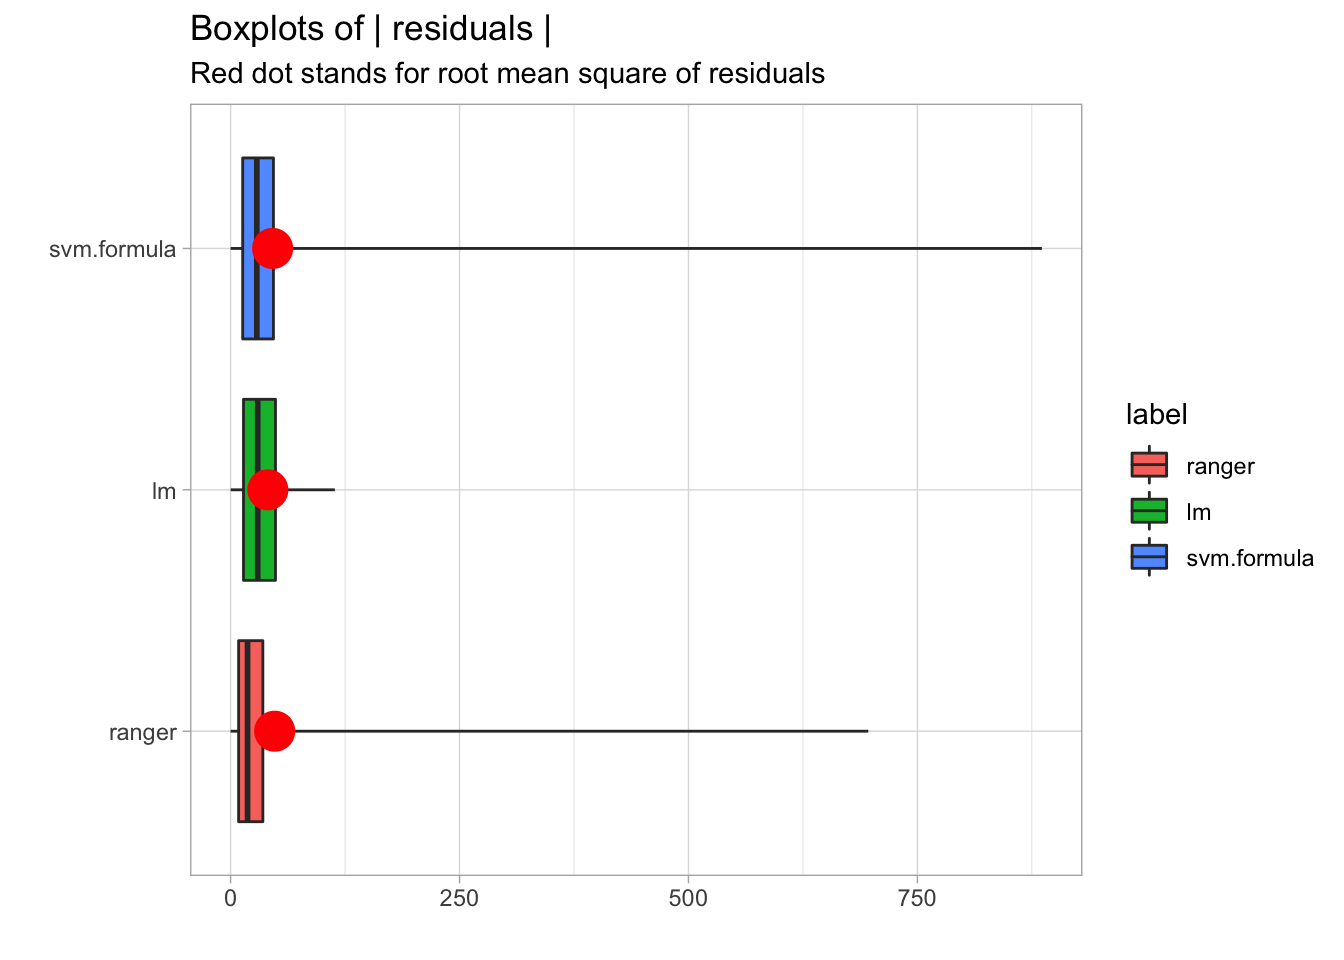
\includegraphics{PM_VEE_files/figure-latex/unnamed-chunk-68-1.pdf}

\hypertarget{comparision-of-prediction-level-explainers}{%
\section{Comparision of prediction level
explainers}\label{comparision-of-prediction-level-explainers}}

TODO

compare pros and cons of different techniques

\hypertarget{when-to-use}{%
\subsection{When to use?}\label{when-to-use}}

There are several use-cases for such explainers. Think about following.

\begin{itemize}
\tightlist
\item
  Model improvement. If model works particular bad for a selected
  observation (the residual is very high) then investigation of model
  responses for miss fitted points may give some hints how to improve
  the model. For individual predictions it is easier to notice that
  selected variable should have different a effect.
\item
  Additional domain specific validation. Understanding which factors are
  important for model predictions helps to be critical about model
  response. If model contributions are against domain knowledge then we
  may be more skeptical and willing to try another model. On the other
  hand, if the model response is aligned with domain knowledge we may
  trust more in these responses. Such trust is important in decisions
  that may lead to serious consequences like predictive models in
  medicine.
\item
  Model selection. Having multiple candidate models one may select the
  final response based on model explanations. Even if one model is
  better in terms of global model performance it may happen that locally
  other model is better fitted. This moves us towards model
  consultations that identify different options and allow human to
  select one of them.
\end{itemize}

Enslaving the Algorithm: From a `Right to an Explanation' to a `Right to
Better Decisions'? \citep{Edwards_Veale_2018}

TODO: Sparse model approximation / variable selection / feature ranking

\hypertarget{model-level-explanations}{%
\section*{Model level explanations}\label{model-level-explanations}}
\addcontentsline{toc}{section}{Model level explanations}

\hypertarget{introduction-6}{%
\section{Introduction}\label{introduction-6}}

Model level explainers help to understand how the model works in
general, for some population of interest. This is the main difference
from the instance level explainers that were focused on a model
behaviour around a single observation. Model level explainers work in
the context of a population or subpopulation.

Think about following use-cases

\begin{itemize}
\tightlist
\item
  One wants to know which variables are important in the model. Think
  about model for heart accident in which features come from additional
  medical examinations. Knowing which examinations are not important one
  can reduce a model by removing unnecessary variables.
\item
  One wants to understand how a selected variable affects the model
  response. Think about a model for prediction of apartment prices. You
  know that apartment location is an important factor, but which
  locations are better and how much a given location is worth? Model
  explainers help to understand how values of a selected variable affect
  the model response.
\item
  One wants to know if there are any unusual observations that do not
  fit to the model. Observations with unusually large residuals. Think
  about a model for survival after some very risky treatment. You would
  like to know if for some patients the model predictions are extremely
  incorrect.
\end{itemize}

All cases mentioned above are linked with either model diagnostic
(checking if model behaves alog our expectations) or knowledge
extraction (model was trained to extract some knowledge about the
discipline).

\hypertarget{approaches-to-model-explanations}{%
\subsection{Approaches to model
explanations}\label{approaches-to-model-explanations}}

Model level explanations are focused on four main aspects of a model.

\begin{itemize}
\tightlist
\item
  Model performance. Here the question is how good is the model, is it
  good enough (better than some predefined threshold), is a model A
  better than model B?
\item
  Variable importance. How important are variables, which are the most
  important and which are not important at all?
\item
  Variable effects. What is the relation between a variable and model
  response, can the variable be transformed to create a better model?
\item
  Model residuals. Is there any unusual pattern related to residuals,
  are they biased, are they correlated with some additional variable?
\end{itemize}

\hypertarget{a-bit-of-philosophy-three-laws-for-model-level-explanations}{%
\subsection{A bit of philosophy: Three Laws for Model Level
Explanations}\label{a-bit-of-philosophy-three-laws-for-model-level-explanations}}

In the spirit of three laws introduces in the chapter
\ref{three-single-laws} here we propose three laws for model level
explanations.

\begin{itemize}
\tightlist
\item
  \textbf{Variable importance.} For every model we shall be able to
  understand which variables are important and which are not.
\item
  \textbf{Model audit.} For every model we shall be able to verify basic
  check like if residuals are correlated with variables and if there are
  unusual observations.
\item
  \textbf{Second opinion.} For every model we shall be able to compare
  it against other models to verify if they capture different stories
  about the data.
\end{itemize}

\hypertarget{variableImportance}{%
\section{Feature Importance}\label{variableImportance}}

Methods presented in this chapter are useful for assessment of feature
importance. There are many possible applications of such methods, for
example:

\begin{itemize}
\tightlist
\item
  Feature importance scores may be used for feature filtering. Features
  that are not important may be removed from the model training
  procedure. Removal of the noise shall lead to better models.
\item
  Identification of the most important features may be used as a
  validation of a model against domain knowledge. Just to make sure that
  it's not like a single random feature dominates model predictions.
\item
  Identification of the most important features may leads to new domain
  knowledge. Well, we have identified important features.
\item
  Comparison of feature importance between different models helps to
  understand how different models handle particular features.
\item
  Ranking of feature importance helps to decide in what order we shall
  perform further model exploration, in what order we shall examine
  particular feature effects.
\end{itemize}

There are many methods for assessment of feature importance. In general
we may divide them into two groups, methods that are model specific and
methods that are model agnostic.

Some models like random forest, gradient boosting, linear models and
many others have their own ways to assess feature importance. Such
method are linked with the particular structure of the model. In terms
of linear models such specific measures are linked with normalized
regression coefficients of p-values. For tree based ensembles such
measures may be based on utilization of particular features in
particular trees, see \citep{xgboostExplainer} for gradient boosting or
\citep{randomForestExplainer} for random forest.

But in this book we are focused on methods that are model agnostic. The
may reason for that is

\begin{itemize}
\tightlist
\item
  First, be able to apply this method to any predictive model or
  ensemble of models.
\item
  Second, (which is maybe even more important) to be able to compare
  feature importance between models despite differences in their
  structure.
\end{itemize}

Model agnostic methods cannot assume anything about the model structure
and we do not want to refit a model. The method that is presented below
is described in details in the \citep{variableImportancePermutations}.
The main idea is to measure how much the model fit will decrease if a
selected feature or group of features will be cancelled out. Here
cancellation means perturbations like resampling from empirical
distribution of just permutation.

The method can be used to measure importance of single features, pairs
of features or larger tuples For the simplicity below we describe
algorithm for single features, but it is straight forward to use it for
larger subsets of features.

\hypertarget{permutation-based-feature-importance}{%
\subsection{Permutation Based Feature
Importance}\label{permutation-based-feature-importance}}

The idea behind is easy and in some sense borrowed from Random Forest
\citep{R-randomForest}. If a feature is important then after permutation
model performance shall drop. The larger drop the more important is the
feature.

Let's describe this idea in a bit more formal way. Let
\(\mathcal L(f(x), y)\) be a loss function that assess goodness of fit
for a model \(f(x)\) while let \(\mathcal X\) be a set of features.

\begin{enumerate}
\def\labelenumi{\arabic{enumi}.}
\tightlist
\item
  For each feature \(x_i \in \mathcal X\) do steps 2-5
\item
  Create a new data \(x^{*,-i}\) with feature \(x_i\) resampled (or
  permutated).
\item
  Calculate model predictions for the new data \(x^{*,-i}\), they will
  be denoted as \(f(x^{*,-i})\).
\item
  Calculate loss function for models predictions on perturbed data \[
  L^{*,-i} = \mathcal L(f(x^{*,-i}), y)
  \]
\item
  Feature importance may be calculated as difference or ratio of the
  original loss and loss on perturbed data, i.e.
  \(vip(x_i) = L^{*,-i} - L\) or \(vip(x_i) = L^{*,-i} / L\).
\end{enumerate}

Note that ranking of feature importance will be the same for the
difference and the ratio since the loss \(L\) is the same.

Note also, that the main advantage of the step 5 is that feature
importance is kind of normalized. But in many cases such normalization
is not needed and in fact it makes more sense to present raw
\(L^{*,-i}\) values.

\hypertarget{example-titanic}{%
\subsection{Example: Titanic}\label{example-titanic}}

Let's use this approach to a random forest model created for the Titanic
dataset. The goal is to predict passenger survival probability based on
their sex, age, class, fare and some other features available in the
\texttt{titanic} dataset.

\begin{Shaded}
\begin{Highlighting}[]
\KeywordTok{head}\NormalTok{(titanic)}
\end{Highlighting}
\end{Shaded}

\begin{verbatim}
##   gender age class    embarked       country  fare sibsp parch survived
## 1   male  42   3rd Southampton United States  7.11     0     0       no
## 2   male  13   3rd Southampton United States 20.05     0     2       no
## 3   male  16   3rd Southampton United States 20.05     1     1       no
## 4 female  39   3rd Southampton       England 20.05     1     1      yes
## 5 female  16   3rd Southampton        Norway  7.13     0     0      yes
## 6   male  25   3rd Southampton United States  7.13     0     0      yes
##   age_cat fare_cat
## 1 (30,50]   (0,10]
## 2 (10,18]  (10,25]
## 3 (10,18]  (10,25]
## 4 (30,50]  (10,25]
## 5 (10,18]   (0,10]
## 6 (18,30]   (0,10]
\end{verbatim}

Permutation based feature importance can be calculated with the
\texttt{feature\_importance\{ingredients\}}. By default it permutes
values feature by feature.

Instead of showing normalized feature importance we plot both original
\(L\) and loss after permutation \(L^{*,-i}\). This way we can read also
how good was the model, and as we will see in next subsection it will be
useful for model comparison.

\begin{Shaded}
\begin{Highlighting}[]
\KeywordTok{library}\NormalTok{(}\StringTok{"ingredients"}\NormalTok{)}
\NormalTok{fi_rf <-}\StringTok{ }\KeywordTok{feature_importance}\NormalTok{(explain_titanic_rf) }
\KeywordTok{plot}\NormalTok{(fi_rf) }\OperatorTok{+}\StringTok{ }\KeywordTok{ggtitle}\NormalTok{(}\StringTok{"Permutation based feature importance"}\NormalTok{, }\StringTok{"For Random Forest model and Titanic data"}\NormalTok{)}
\end{Highlighting}
\end{Shaded}

\begin{figure}
\centering
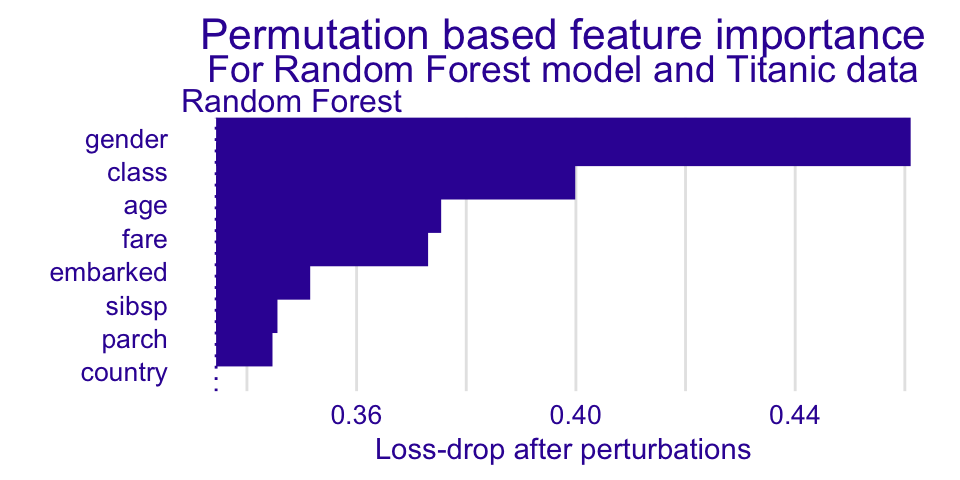
\includegraphics{PM_VEE_files/figure-latex/titanic3-1.pdf}
\caption{\label{fig:titanic3}Feature importance. Each interval presents the
difference between original model performance (left end) and the
performance on a dataset with a single feature perturbed}
\end{figure}

It's interesting that the most important variable for Titanic data is
the Sex. So it have been ,,women first'' after all. Then the three
features of similar importance are passenger class (first class has
higher survival), age (kids have higher survival) and fare (owners of
more pricy tickets have higher survival).

Note that drawing permutations evolves some randomness. Thus to have
higher repeatability of results you may either set a seed for random
number generator or replicate the procedure few times. The second
approach has additional advantage, that you will learn the uncertainty
behind feature importance assessment.

Here we present scores for 10 repetition of the process.

\begin{Shaded}
\begin{Highlighting}[]
\NormalTok{fi_rf10 <-}\StringTok{ }\KeywordTok{replicate}\NormalTok{(}\DecValTok{10}\NormalTok{, }\KeywordTok{feature_importance}\NormalTok{(explain_titanic_rf), }\DataTypeTok{simplify =} \OtherTok{FALSE}\NormalTok{)}
\KeywordTok{do.call}\NormalTok{(plot, fi_rf10) }\OperatorTok{+}\StringTok{ }\KeywordTok{ggtitle}\NormalTok{(}\StringTok{"Permutation based feature importance"}\NormalTok{, }\StringTok{"For Random Forest model and Titanic data"}\NormalTok{)}
\end{Highlighting}
\end{Shaded}

\begin{figure}
\centering
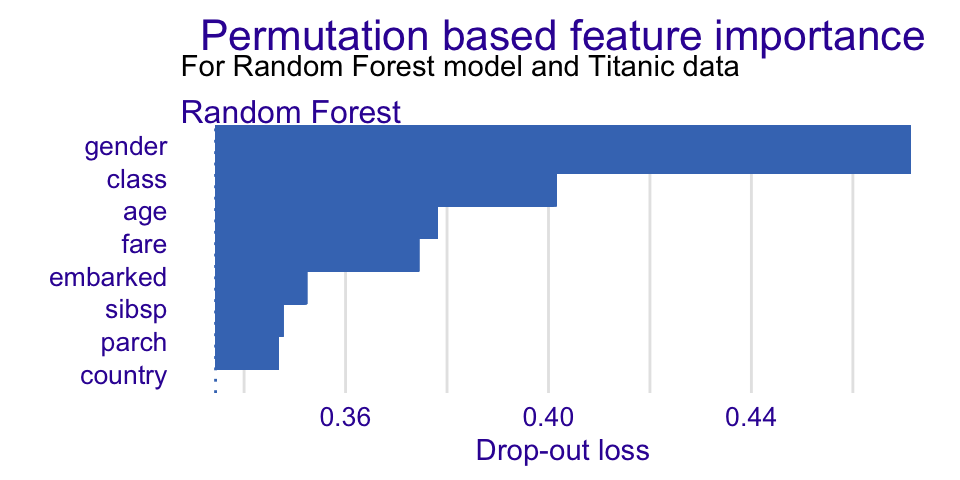
\includegraphics{PM_VEE_files/figure-latex/titanic4-1.pdf}
\caption{\label{fig:titanic4}Feature importance for 10 replication of
feature importance assessment}
\end{figure}

It is much easier to assess feature importance if they come with some
assessment of the uncertainty. We can read from the plot that Age and
passenger class are close to each other.

Note that intervals are useful for model comparisons. In the Figure
@ref\{titanic5\} we can read feature importance for random forest,
gradient boosting and logistic regression models. Best results are
achieved by the random forest model and also this method consume more
features than others. A good example is the \emph{Fare} variable, not
used in gradient boosting not logistic regression (as a feature highly
correlated with passenger class) but consumed in the random forest
model.

\begin{Shaded}
\begin{Highlighting}[]
\NormalTok{fi_rf <-}\StringTok{ }\KeywordTok{feature_importance}\NormalTok{(explain_titanic_rf)}
\NormalTok{fi_gbm <-}\StringTok{ }\KeywordTok{feature_importance}\NormalTok{(explain_titanic_gbm)}
\NormalTok{fi_glm <-}\StringTok{ }\KeywordTok{feature_importance}\NormalTok{(explain_titanic_lmr)}

\KeywordTok{plot}\NormalTok{(fi_rf, fi_gbm, fi_glm)}
\end{Highlighting}
\end{Shaded}

\begin{figure}
\centering
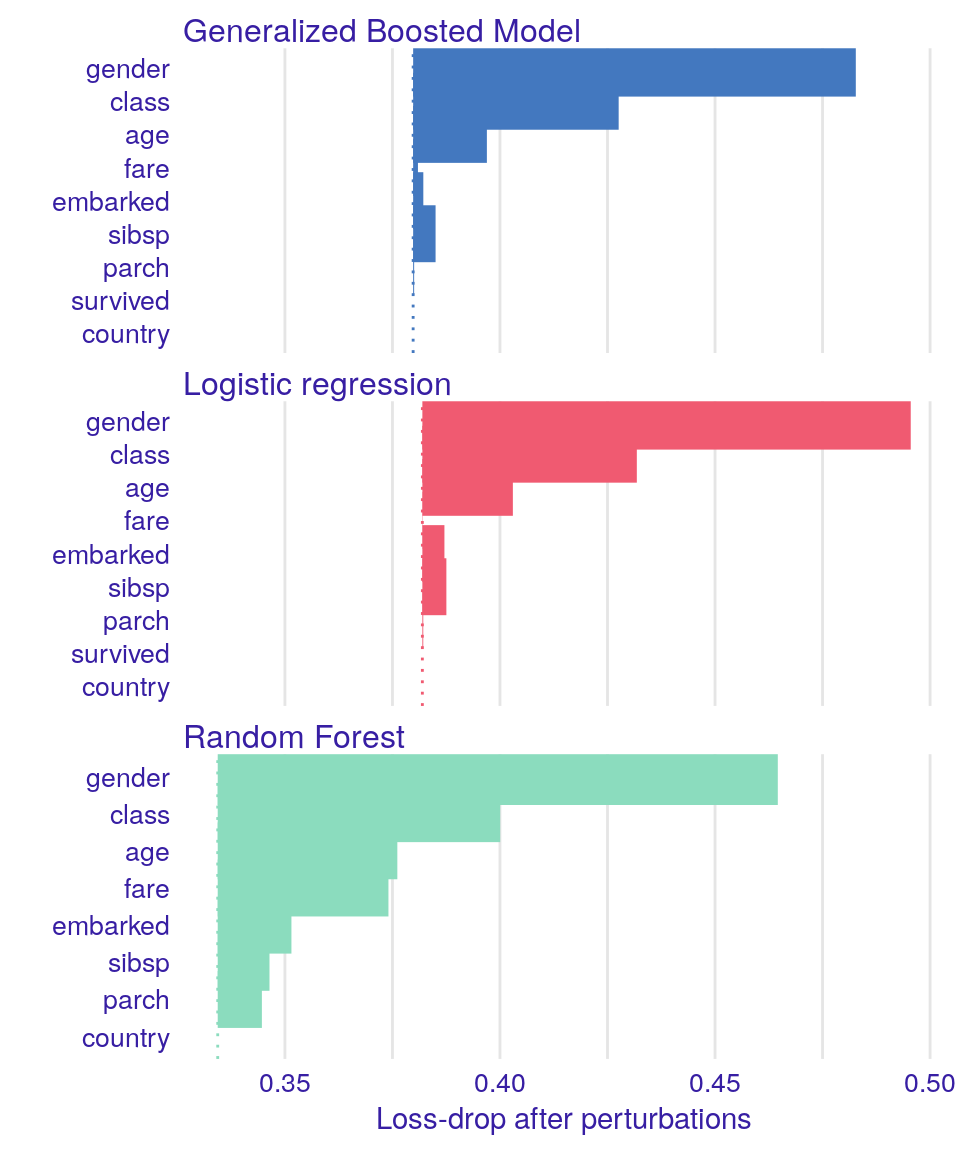
\includegraphics{PM_VEE_files/figure-latex/titanic5-1.pdf}
\caption{\label{fig:titanic5}Feature importance for random forest, gradient
boosting and logistic regression models}
\end{figure}

\hypertarget{example-price-prediction}{%
\subsection{Example: Price prediction}\label{example-price-prediction}}

Let's create a regression model for prediction of apartment prices.

\begin{Shaded}
\begin{Highlighting}[]
\KeywordTok{library}\NormalTok{(}\StringTok{"DALEX"}\NormalTok{)}
\KeywordTok{library}\NormalTok{(}\StringTok{"randomForest"}\NormalTok{)}
\KeywordTok{set.seed}\NormalTok{(}\DecValTok{59}\NormalTok{)}
\NormalTok{model_rf <-}\StringTok{ }\KeywordTok{randomForest}\NormalTok{(m2.price }\OperatorTok{~}\StringTok{ }\NormalTok{construction.year }\OperatorTok{+}\StringTok{ }\NormalTok{surface }\OperatorTok{+}\StringTok{ }\NormalTok{floor }\OperatorTok{+}\StringTok{ }
\StringTok{                           }\NormalTok{no.rooms }\OperatorTok{+}\StringTok{ }\NormalTok{district, }\DataTypeTok{data =}\NormalTok{ apartments)}
\end{Highlighting}
\end{Shaded}

A popular loss function for regression model is the root mean square
loss \[
  L(x, y) = \sqrt{\frac1n \sum_{i=1}^n (x_i - y_i)^2}
\]

\begin{Shaded}
\begin{Highlighting}[]
\KeywordTok{loss_root_mean_square}\NormalTok{(}
  \KeywordTok{predict}\NormalTok{(model_rf, apartments), }
\NormalTok{  apartments}\OperatorTok{$}\NormalTok{m2.price}
\NormalTok{)}
\end{Highlighting}
\end{Shaded}

\begin{verbatim}
## [1] 193.8477
\end{verbatim}

Let's calculate feature importance

\begin{Shaded}
\begin{Highlighting}[]
\NormalTok{explainer_rf <-}\StringTok{ }\KeywordTok{explain}\NormalTok{(model_rf, }
            \DataTypeTok{data =}\NormalTok{ apartmentsTest[,}\DecValTok{2}\OperatorTok{:}\DecValTok{6}\NormalTok{], }\DataTypeTok{y =}\NormalTok{ apartmentsTest}\OperatorTok{$}\NormalTok{m2.price)}
\NormalTok{vip <-}\StringTok{ }\KeywordTok{variable_importance}\NormalTok{(explainer_rf, }
            \DataTypeTok{loss_function =}\NormalTok{ loss_root_mean_square)}
\NormalTok{vip}
\end{Highlighting}
\end{Shaded}

\begin{verbatim}
##            variable dropout_loss        label
## 1      _full_model_     285.1355 randomForest
## 2          no.rooms     391.0710 randomForest
## 3 construction.year     410.5866 randomForest
## 4             floor     445.2164 randomForest
## 5           surface     480.1431 randomForest
## 6          district     843.6519 randomForest
## 7        _baseline_    1081.3710 randomForest
\end{verbatim}

On a diagnostic plot is useful to present feature importance as an
interval that start in a loss and ends in a loss of perturbed data.

\begin{Shaded}
\begin{Highlighting}[]
\KeywordTok{plot}\NormalTok{(vip)}
\end{Highlighting}
\end{Shaded}

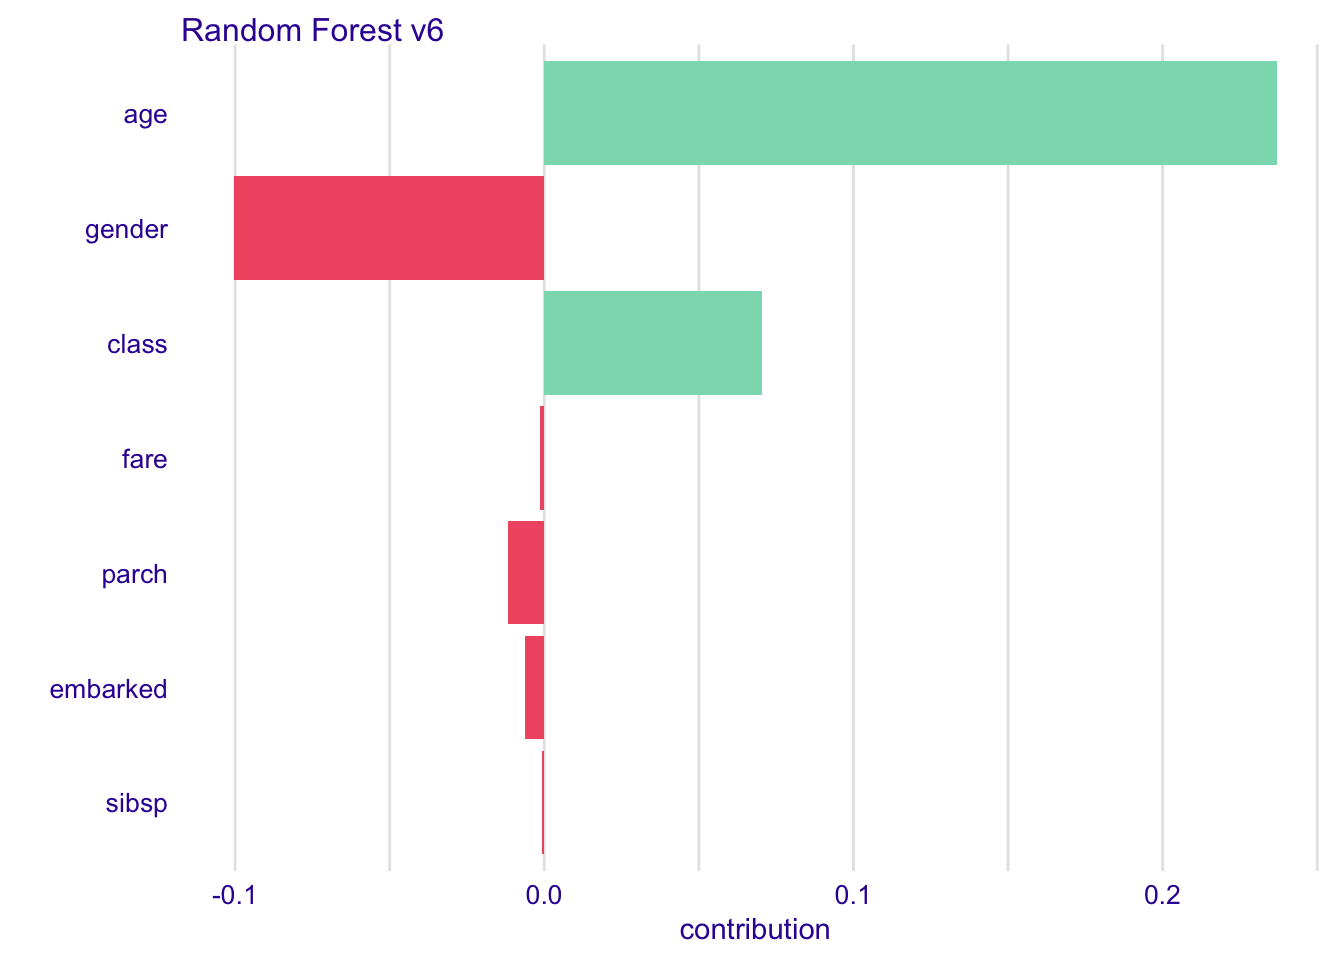
\includegraphics{PM_VEE_files/figure-latex/unnamed-chunk-72-1.pdf}

\hypertarget{more-models}{%
\subsection{More models}\label{more-models}}

Much more can be read from feature importance plots if we compare models
of a different structure. Let's train three predictive models trained on
\texttt{apartments} dataset from the \texttt{DALEX} package. Random
Forest model \citep{R-randomForest} (elastic but biased), Support Vector
Machines model \citep{R-e1071} (large variance on boundaries) and Linear
Model (stable but not very elastic). Presented examples are for
regression (prediction of square meter price), but the CP profiles may
be used in the same way for classification.

Let's fit these three models.

\begin{Shaded}
\begin{Highlighting}[]
\KeywordTok{library}\NormalTok{(}\StringTok{"DALEX"}\NormalTok{)}
\NormalTok{model_lm <-}\StringTok{ }\KeywordTok{lm}\NormalTok{(m2.price }\OperatorTok{~}\StringTok{ }\NormalTok{construction.year }\OperatorTok{+}\StringTok{ }\NormalTok{surface }\OperatorTok{+}\StringTok{ }\NormalTok{floor }\OperatorTok{+}\StringTok{ }
\StringTok{                      }\NormalTok{no.rooms }\OperatorTok{+}\StringTok{ }\NormalTok{district, }\DataTypeTok{data =}\NormalTok{ apartments)}

\KeywordTok{library}\NormalTok{(}\StringTok{"randomForest"}\NormalTok{)}
\KeywordTok{set.seed}\NormalTok{(}\DecValTok{59}\NormalTok{)}
\NormalTok{model_rf <-}\StringTok{ }\KeywordTok{randomForest}\NormalTok{(m2.price }\OperatorTok{~}\StringTok{ }\NormalTok{construction.year }\OperatorTok{+}\StringTok{ }\NormalTok{surface }\OperatorTok{+}\StringTok{ }\NormalTok{floor }\OperatorTok{+}\StringTok{ }
\StringTok{                      }\NormalTok{no.rooms }\OperatorTok{+}\StringTok{ }\NormalTok{district, }\DataTypeTok{data =}\NormalTok{ apartments)}

\KeywordTok{library}\NormalTok{(}\StringTok{"e1071"}\NormalTok{)}
\NormalTok{model_svm <-}\StringTok{ }\KeywordTok{svm}\NormalTok{(m2.price }\OperatorTok{~}\StringTok{ }\NormalTok{construction.year }\OperatorTok{+}\StringTok{ }\NormalTok{surface }\OperatorTok{+}\StringTok{ }\NormalTok{floor }\OperatorTok{+}\StringTok{ }
\StringTok{                         }\NormalTok{no.rooms }\OperatorTok{+}\StringTok{ }\NormalTok{district, }\DataTypeTok{data =}\NormalTok{ apartments)}
\end{Highlighting}
\end{Shaded}

For these models we use \texttt{DALEX} explainers created with
\texttt{explain()} function. These explainers wrap models, predict
functions and validation data.

\begin{Shaded}
\begin{Highlighting}[]
\NormalTok{explainer_lm <-}\StringTok{ }\KeywordTok{explain}\NormalTok{(model_lm, }
                       \DataTypeTok{data =}\NormalTok{ apartmentsTest[,}\DecValTok{2}\OperatorTok{:}\DecValTok{6}\NormalTok{], }\DataTypeTok{y =}\NormalTok{ apartmentsTest}\OperatorTok{$}\NormalTok{m2.price)}
\NormalTok{vip_lm <-}\StringTok{ }\KeywordTok{variable_importance}\NormalTok{(explainer_lm, }
            \DataTypeTok{loss_function =}\NormalTok{ loss_root_mean_square)}
\NormalTok{vip_lm}
\end{Highlighting}
\end{Shaded}

\begin{verbatim}
##            variable dropout_loss label
## 1      _full_model_     282.0062    lm
## 2 construction.year     281.9007    lm
## 3          no.rooms     292.8398    lm
## 4             floor     492.0857    lm
## 5           surface     614.9198    lm
## 6          district    1002.3487    lm
## 7        _baseline_    1193.6209    lm
\end{verbatim}

\begin{Shaded}
\begin{Highlighting}[]
\NormalTok{explainer_rf <-}\StringTok{ }\KeywordTok{explain}\NormalTok{(model_rf, }
                       \DataTypeTok{data =}\NormalTok{ apartmentsTest[,}\DecValTok{2}\OperatorTok{:}\DecValTok{6}\NormalTok{], }\DataTypeTok{y =}\NormalTok{ apartmentsTest}\OperatorTok{$}\NormalTok{m2.price)}
\NormalTok{vip_rf <-}\StringTok{ }\KeywordTok{variable_importance}\NormalTok{(explainer_rf, }
            \DataTypeTok{loss_function =}\NormalTok{ loss_root_mean_square)}
\NormalTok{vip_rf}
\end{Highlighting}
\end{Shaded}

\begin{verbatim}
##            variable dropout_loss        label
## 1      _full_model_     293.2729 randomForest
## 2          no.rooms     389.4526 randomForest
## 3 construction.year     416.1154 randomForest
## 4             floor     453.9195 randomForest
## 5           surface     480.4062 randomForest
## 6          district     867.7050 randomForest
## 7        _baseline_    1116.2616 randomForest
\end{verbatim}

\begin{Shaded}
\begin{Highlighting}[]
\NormalTok{explainer_svm <-}\StringTok{ }\KeywordTok{explain}\NormalTok{(model_svm, }
                       \DataTypeTok{data =}\NormalTok{ apartmentsTest[,}\DecValTok{2}\OperatorTok{:}\DecValTok{6}\NormalTok{], }\DataTypeTok{y =}\NormalTok{ apartmentsTest}\OperatorTok{$}\NormalTok{m2.price)}
\NormalTok{vip_svm <-}\StringTok{ }\KeywordTok{variable_importance}\NormalTok{(explainer_svm, }
            \DataTypeTok{loss_function =}\NormalTok{ loss_root_mean_square)}
\NormalTok{vip_svm}
\end{Highlighting}
\end{Shaded}

\begin{verbatim}
##            variable dropout_loss label
## 1      _full_model_     157.7938   svm
## 2          no.rooms     221.4595   svm
## 3 construction.year     365.2600   svm
## 4             floor     439.8724   svm
## 5           surface     527.2598   svm
## 6          district     942.8512   svm
## 7        _baseline_    1203.7571   svm
\end{verbatim}

Let's plot feature importance for all three models on a single plot.

Intervals start in a different values, thus we can read that loss for
SVM model is the lowest.

When we compare other features it looks like in all models the
\texttt{district} is the most important feature followed by
\texttt{surface} and \texttt{floor}.

\begin{Shaded}
\begin{Highlighting}[]
\KeywordTok{plot}\NormalTok{(vip_rf, vip_svm, vip_lm)}
\end{Highlighting}
\end{Shaded}

\includegraphics{PM_VEE_files/figure-latex/unnamed-chunk-75-1.pdf}

There is interesting difference between linear model and others in the
way how important is the \texttt{construction.year}. For linear model
this variable is not importance, while for remaining two models there is
some importance.

In the next chapter we will see how this is possible.

\hypertarget{level-frequency}{%
\subsection{Level frequency}\label{level-frequency}}

What does the feature importance mean? How it is linked with a data
distribution.

\hypertarget{variableEngeneering}{%
\section{Feature effects}\label{variableEngeneering}}

In following chapters we introduce tools for extraction of the
information between model response and individual model inputs. These
tools are useful to summarize how ,,in general'' model responds to the
input of interest. All presented approaches are based on Ceteris Ceteris
Paribus Profiles introduced in Chapter @ref\{ceterisParibus\} but they
differ in a way how individual profiles are merged into a global model
response.

We use the term ,,feature effect'' to refer to global model response as
a function of single or small number of model features. Methods
presented in this chapter are useful for extraction information of
feature effect, i.e.~how a feature is linked with model response. There
are many possible applications of such methods, for example:

\begin{itemize}
\tightlist
\item
  Feature effect may be used for feature engineering. The crude approach
  to modeling is to fit some elastic model on raw data and then use
  feature effects to understand the relation between a raw feature and
  model output and then to transform model input to better fit the model
  output. Such procedure is called surrogate training. In this procedure
  an elastic model is trained to learn about link between a feature and
  the target. Then a new feature is created in a way to better utilized
  the feature in a simpler model \citep{SAFE-arxiv}. In the next
  chapters we will show how feature effects can be used to transform a
  continuous variable in to a categorical one in order to improve the
  model behavior.
\item
  Feature effect may be used for model validation. Understanding how a
  model utilizes a feature may be used as a validation of a model
  against domain knowledge. For example if we expect monotonic relation
  or linear relation then such expectations can be verified. Also if we
  expect smooth relation between model and its inputs then the
  smoothness can be visually examined. In the next chapters we will show
  how feature effects can be used to warn a model developer that model
  is unstable and should be regularized.
\item
  In new domains an understanding of a link between model output and the
  feature of interest may increase our domain knowledge. It may give
  quick insights related to the strength or character of the relation
  between a feature of interest and the model output.
\item
  The comparison of feature effects between different models may help to
  understand how different models handle particular features. In the
  next chapters we will show how feature effects can be used learn
  limitations of particular classes of models.
\end{itemize}

\hypertarget{global-level-vs-instance-level-explanations}{%
\subsection{Global level vs instance level
explanations}\label{global-level-vs-instance-level-explanations}}

The plot below shows Ceteris Paribus Profiles for the random forest
\texttt{rf\_5} for 10 selected passengers. Different profiles behave
differently. In following chapter we discuss different approaches to
aggregation of such profiles into model level feature effects.

\begin{figure}
\centering
\includegraphics{PM_VEE_files/figure-latex/pdp_part_1A-1.pdf}
\caption{(\#fig:pdp\_part\_1A)Ceteris Paribus profiles for 10 passangers
and the random forest model}
\end{figure}

\hypertarget{partialDependenceProfiles}{%
\section{Partial Dependency Profiles}\label{partialDependenceProfiles}}

One of the first and the most popular tools for inspection of black-box
models on the global level are Partial Dependence Plots (sometimes
called Partial Dependence Profiles).

PDP were introduced by Friedman in 2000 in his paper devoted to Gradient
Boosting Machines (GBM) - new type of complex yet effective models
\citep{Friedman00greedyfunction}. For many years PDP as sleeping
beauties stay in the shadow of the boosting method. But this has changed
in recent years. PDP are very popular and available in most of data
science languages. In this chapter we will introduce key intuitions,
explain the math beyond PDP and discuss strengths and weaknesses.

General idea is to show how the expected model response behaves as a
function of a selected feature. Here the term ,,expected'' will be
estimated simply as the average over the population of individual
Ceteris Paribus Profiles introduced in \ref{ceterisParibus}.

\hypertarget{definition}{%
\subsection{Definition}\label{definition}}

Partial Dependency Profile for for a model \(f\) and a variable \(x^j\)
is defined as

\[
g_{PD}^{f, j}(z) = E[f(x^j=z, X^{-j})] = E[f(x|^j=z)].
\]

So it's an expected value for \(x^j = z\) over \textbf{marginal}
distribution \(X^{-j}\) or equivalently expected value of \(f\) after
variable \(x^j\) is set to \(z\).

\emph{Exercise}

Let \(f = x_1 + x_2\) and distribuion of \((x_1, x_2)\) is given by
\(x_1 \sim U[0,1]\) and \(x_2=x_1\).

Calculate \(g_{PD}^{f, 1}(z)\).

\emph{Answer} \(g_{PD}^{f, 1}(z) = z + 0.5\).

\hypertarget{estimation}{%
\subsection{Estimation}\label{estimation}}

Let's see how they are constructed step by step. Here we will use a
random forest \texttt{rf\_5} model for the \emph{titanic} dataset.
Examples are related to a single variable \emph{age}.

The expectation cannot be calculated directly as we do not know fully
neither the distribution of \(X^{-j}\) nor the \(f()\). Yet this value
may be estimated by as average from CP profiles.

\[
\hat g_{PD}^{f, j}(z) = \frac 1n \sum_{i=1}^{N} f(x_i^j=z, x^{-j}_i)] = \frac 1n \sum_{i=1}^{N} f(x_i|^j=z).
\]

\begin{enumerate}
\def\labelenumi{\arabic{enumi}.}
\tightlist
\item
  Calculate Ceteris Paribus Profiles for observations from the dataset
\end{enumerate}

As it was introduced in @ref\{ceterisParibus\} Ceteris Paribus profiles
are calculated for observations. They show how model response change is
a selected variable in this observation is modified.

\[
CP^{f, j, x}(z) := f(x|^j = z).
\]

Such profiles can be calculated for example with the
\texttt{ceteris\_paribus\{ingredients\}} function.

\begin{figure}
\centering
\includegraphics{PM_VEE_files/figure-latex/pdp_part_1-1.pdf}
\caption{(\#fig:pdp\_part\_1)Ceteris Paribus profiles for 100
observations, the age variable and the random forest model}
\end{figure}

So for a single model and a single variable we get a bunch of
\emph{what-if} profiles. In the figure @ref\{pdp\_part\_1\} we show an
example for 100 observations. Despite some variation (random forest are
not as stable as we would hope) we see that most profiles are
decreasing. So the older the passengers is the lower is the survival
probability.

\begin{enumerate}
\def\labelenumi{\arabic{enumi}.}
\setcounter{enumi}{1}
\tightlist
\item
  Aggregate Ceteris Paribus into a single Partial Dependency Profile
\end{enumerate}

Simple pointwise average across CP profiles. If number of CPprofiles is
large, it is enoug to sample some number of them to get resonably
accurate PD profiles.

Here we show profiles calculated with \texttt{ingredients} package, but
find siilar implementation in the \texttt{pdp} package \citep{pdp},
\texttt{ALEPlots} package \citep{R-ALEPlot} or \texttt{iml} \citep{iml}
package.

Such average can be calculated with the
\texttt{aggregate\_profiles\{ingredients\}} function.

\begin{Shaded}
\begin{Highlighting}[]
\NormalTok{pdp_rf <-}\StringTok{ }\KeywordTok{aggregate_profiles}\NormalTok{(cp_rf)}
\KeywordTok{plot}\NormalTok{(pdp_rf) }\OperatorTok{+}
\StringTok{  }\KeywordTok{ggtitle}\NormalTok{(}\StringTok{"Partial Dependency profile"}\NormalTok{, }\StringTok{"For a random forest model / Titanic data"}\NormalTok{) }
\end{Highlighting}
\end{Shaded}

\includegraphics{PM_VEE_files/figure-latex/unnamed-chunk-76-1.pdf}

So for a single model and a single variable we get a profile. See an
example in figure @ref\{pdp\_part\_2\}. It is much easier than following
100 separate curves, and in cases in which Ceteris Paribus are more or
less parallel, the Partial Dependency is a good summary of them.

The average response is of course more stable (as it's an average) and
in this case is more or less a decreasing curve. It's much easier to
notice that the older the passenger is the lower the survival
probability. Moreover it is easier to notice that the largest drop in
survival changes happen for teenagers. On average the survival for
adults is 30 percent points smaller than for kids.

\begin{figure}
\centering
\includegraphics{PM_VEE_files/figure-latex/pdp_part_2-1.pdf}
\caption{(\#fig:pdp\_part\_2)Partial Dependency profile as an average
for 100 observations}
\end{figure}

\hypertarget{clustered-partial-dependency-profiles}{%
\subsection{Clustered Partial Dependency
Profiles}\label{clustered-partial-dependency-profiles}}

As we said in the previous section, Partial Dependency is a good summary
if Ceteris Paribus profiles are similar, i.e.~parallel. But it may
happen that the variable of interest is in interaction with some other
variable. Then profiles are not parallel because the effect of variable
of interest depends on some other variables.

So on one hand it would be good to summaries all this Ceteris Paribus
profiles with smaller number of profiles. But on another hand a single
aggregate may not be enough. To deal with this problem we propose to
cluster Ceteris Paribus profiles and check how homogenous are these
profiles.

The most straightforward approach would be to use a method for
clustering, like k-means algorithm or hierarchical clustering, and see
how these cluster of profiles behave. Once clusters are established we
can aggregate within clusters in the same way as in case of Partial
Dependency Plots.

Such clusters can be calculated with the
\texttt{cluster\_profiles\{ingredients\}} function. We choose the
hierarchical clustering with Ward linkage as it gives most stable
results.

So for a single model and a single variable we get \(k\) profiles. The
common problem in clustering is the selection of \(k\). However in our
case, as it's an exploration, the problem is simpler, as we are
interesting if \(k=1\) (Partial Dependency is a good summary) or not
(there are some interactions).

See an example in Figure @ref\{pdp\_part\_4\}. It is easier to notice
that Ceteris Paribus profiles can be groups in three clusters. Group of
passengers with a very large drop in the survival (cluster 1), moderate
drop (cluster 2) and almost no drop in survival (cluster 3). Here we do
not know what other factors are linked with these clusters, but some
additional exploratory analysis can be done to identify these factors.

\begin{figure}
\centering
\includegraphics{PM_VEE_files/figure-latex/pdp_part_4-1.pdf}
\caption{(\#fig:pdp\_part\_4)Cluster profiles for 3 clusters over 100
Ceteris Paribus profiles}
\end{figure}

\hypertarget{grouped-partial-dependency-profiles}{%
\subsection{Grouped Partial Dependency
Profiles}\label{grouped-partial-dependency-profiles}}

Once we see that variable of interest may be in interaction with some
other variable, it is tempting to look for the factor that distinguish
clusters.

The most straightforward approach is to use some other variable as a
grouping variable. This can be done by setting the \texttt{groups}
argument in the \texttt{aggregate\_profiles\{ingredients\}} function.

\begin{Shaded}
\begin{Highlighting}[]
\KeywordTok{library}\NormalTok{(}\StringTok{"ingredients"}\NormalTok{)}
\NormalTok{selected_passangers <-}\StringTok{ }\KeywordTok{select_sample}\NormalTok{(titanic, }\DataTypeTok{n =} \DecValTok{100}\NormalTok{)}
\NormalTok{cp_rf <-}\StringTok{ }\KeywordTok{ceteris_paribus}\NormalTok{(explain_titanic_rf, selected_passangers)}
\NormalTok{pdp_Sex_rf <-}\StringTok{ }\KeywordTok{aggregate_profiles}\NormalTok{(cp_rf, }\DataTypeTok{variables =} \StringTok{"age"}\NormalTok{,}
                \DataTypeTok{groups =} \StringTok{"gender"}\NormalTok{)}
\end{Highlighting}
\end{Shaded}

See an example in Figure @ref\{pdp\_part\_5\}. Clearly there is an
interaction between Age and Sex. The survival for woman is more stable,
while for man there is more sudden drop in Survival for older
passengers. Check how the interaction for \texttt{Pclass} (passenger
class) looks like.

\begin{figure}
\centering
\includegraphics{PM_VEE_files/figure-latex/pdp_part_5-1.pdf}
\caption{(\#fig:pdp\_part\_5)Grouped profiles with respect to the gender
variable}
\end{figure}

\hypertarget{contrastive-model-comparisons}{%
\subsection{Contrastive Model
Comparisons}\label{contrastive-model-comparisons}}

Contrastive comparisons of Partial Dependency Plots are useful not only
for subgroups of observations but also for model comparisons.

Why one would like to compare models? There are at least three reasons
for it.

\begin{itemize}
\tightlist
\item
  \emph{Agreement of models will calm us.} Some models are known to be
  more stable other to be more elastic. If profiles for models from
  these two classes are not far from each other we can be more convinced
  that elastic model is not over-fitted.
\item
  \emph{Disagreement of models helps to improve.} If simpler
  interpretable model disagree with an elastic model, this may suggest a
  feature transformation that can be used to improve the interpretable
  model. For example if random forest learned non linear relation then
  it can be captures by a linear model after suitable transformation.
\item
  \emph{Validation of boundary conditions.} Some models are know to have
  different behavior on the boundary, for largest or lowest values.
  Random forest is known to shrink predictions towards the average,
  while support vector machines are known to have larger variance at
  edges. Contrastive comparisons may help to understand differences in
  boundary behavior.
\end{itemize}

Generic \texttt{plot\{ingredients\}} function handles multiple models as
consecutive arguments.

See an example in Figure @ref\{pdp\_part\_7\}. Random forest is compared
with gradient boosting model and generalized linear model (logistic
regression). All three models agree when it comes to a general relation
between Age and Survival. Logistic regression is of course the most
smooth. Gradient boosting has on average higher predictions than random
forest.

\begin{figure}
\centering
\includegraphics{PM_VEE_files/figure-latex/pdp_part_7-1.pdf}
\caption{(\#fig:pdp\_part\_7)Comparison on three predictive models with
different structures.}
\end{figure}

\hypertarget{conditionalProfiles}{%
\section{Conditional Dependency Profiles}\label{conditionalProfiles}}

One of the largest advantages of the Partial Dependency Profiles is that
they are easy to explain, as they are just an average across Ceteris
Paribus profiles. But one of the largest disadvantages lies in
expectation over marginal distribution which implies that \(x^j\) is
independent from \(x^{-j}\). In many applications this assumption is
violated. For example, for the \emph{apartments} dataset one can expect
that features like \(surface\) and \(number.or.rooms\) are strongly
correlated as apartments with larger number of rooms usually have larger
surface. It may makes no sense to consider an apartment with 10 rooms
and 20 square meters, so it may be misleading to change \(x^{surface}\)
independently from \(x^{number.of.rooms}\). In the \texttt{titanic}
dataset we shall expect correlation between \texttt{fare} and
\texttt{passanger\ class} as tickets in the 1st class are the most
expensive.

There are several attempts to fix this problem. Here we introduce Local
Dependency Profiles presented in the \citep{R-ALEPlot} under the name
M-profiles.

The general idea is to use conditional distribution instead of marginal
distribution to accomodate for the dependency between \(x^j\) and
\(x^{-j}\).

\hypertarget{definition-1}{%
\subsection{Definition}\label{definition-1}}

Conditional Dependency Profile for a model \(f\) and a variable \(x^j\)
is defined as

\[
g_{CD}^{f, j}(z) = E[f(X^j, X^{-j})|X^j = z].
\]

So it's an expected value over \textbf{conditional} distribution
\((X^j,X^{-j})|X^j=z\).

\emph{Exercise}

Let \(f = x_1 + x_2\) and distribuion of \((x_1, x_2)\) is given by
\(x_1 \sim U[0,1]\) and \(x_2=x_1\).

Calculate \(g_{CD}^{f, 1}(z)\).

\emph{Answer} \(g_{CD}^{f, 1}(z) = 2*z\).

\hypertarget{estimation-1}{%
\subsection{Estimation}\label{estimation-1}}

Partial Dependency Profiles are defined as an expected value from
Ceteris Paribus Profiles.

\[
g^{PD}_i(z) = E_{X_{-i}}[ f(x|^i = z, x^{-i}) ].
\] And can be estimated as average from CP profiles.

\[
\hat g^{PD}_i(z) = \frac{1}{n} \sum_{j=1}^{n} f(x|^i = z, x_j^{-i}).
\]

As it was said, if \(X_i\) and \(X_{-i}\) are related it may have no
sense to average CP profiles over marginal \(X_{-i}\). Instead, an
intuitive approach would to use a conditional distribution
\(X_{-i}|X_i=x_i\).

\[
g^{M}_i(z) = E_{X_{-i}|X_i=x_i}[ f(x|^i = z, x^{-i}) ].
\]

\hypertarget{example}{%
\subsection{Example}\label{example}}

See Figure \ref{accumulatedCor} for illustration of difference between
marginal and conditional distribution. Such profiles are called
Conditional Dependency Profiles and are estimated as

\[
\hat g^{M}_i(z) = \frac{1}{|N_i|} \sum_{j\in N_i} f(x|^i = z, x_j^{-i}). 
\] where \(N_i\) is the set of observations with \(x_i\) close to \(z\).

\begin{figure}

{\centering \includegraphics[width=0.4\linewidth]{figure/CP_ALE_2} 

}

\caption{(fig:accumulatedCor) }\label{fig:accumulatedCor}
\end{figure}

As it is justified in \citep{R-ALEPlot}, there is a serious problem with
this approach, illustrated by a following observation. If \(y\) depends
on \(x_2\) but not \(x_1\) then the correlation between \(x_1\) and
\(x_2\) will produce a \emph{false} relation in the Marginal profiles
for feature \(x_1\). This problem is also illustrated in the Figure
\ref{accumulatedLocalEffects}.

\begin{figure}
\centering
\includegraphics{PM_VEE_files/figure-latex/mp_part_1-1.pdf}
\caption{(\#fig:mp\_part\_1)Conditional Dependency Profile for 100
observations}
\end{figure}

\hypertarget{accumulatedLocalProfiles}{%
\section{Accumulated Local Profiles}\label{accumulatedLocalProfiles}}

As we showed in the previous chapter, Conditional Dependency Profiles
takes into account dependency between features, but it is both advantage
and disadvantage. The advantage is that in some cases the dependency is
real and should be taken into account when computing expected value of
\(f\). The disadvantage is that in the Conditional Dependency Profiles
we see both effects of the feature of interest \(x^j\) and other
features that are dependent on it. Accumulated Local Profiles
disentangle effects of a feature of interest and features correlated
with it.

For example, for the \emph{apartments} dataset one can expect that
features like \(surface\) and \(number.or.rooms\) are correlated but we
can also imagine that each of these variables affect the apartment price
somehow. Partial Dependency Profiles show how the average price changes
as a function of surface, keeping all other variables unchanged.
Conditional Dependency Profiles show how the average price changes as a
function of surface adjusting all other variables to the current value
of the surface. Accumulated Local Profiles show how the average price
changes as a function of surface adjusting all other variables to the
current value of the surface but extracting changes caused by these
other features.

Accumulated Local Dependency Profiles presented in the \citep{R-ALEPlot}
paper.

The general idea is to accumulate local changes in model response
affected by single feature \(x^j\).

\hypertarget{definition-2}{%
\subsection{Definition}\label{definition-2}}

Accumulated Local Profile for a model \(f\) and a variable \(x^j\) is
defined as

\[
g_{AL}^{f, j}(z) = \int_{z_0}^z E\left[\frac{\partial f(X^j, X^{-j})}{\partial x_j}|X^j = v\right] dv + c,
\] where \(z_0\) if the lower boundry of \(x^j\). The profile
\(g_{AL}^{f, j}(z)\) is calculated up to some constant \(c\). Usually
the constant \(c\) is selected to keep average \(g_{AL}^{f, j}\) equal
to 0 or average \(f\).

The equation may be a bit complex, but the intuition is not that
complicated. Instead of aggregation of Ceteris Paribus we just look
locally how quickly CP profiles are changing. And AL profile is
reconstructed from such local partial changes.

So it's an cummulated expected change of the model response along where
the expected values are calculated over \textbf{conditional}
distribution \((X^j,X^{-j})|X^j=v\).

\emph{Exercise}

Let \(f = x_1 + x_2\) and distribuion of \((x_1, x_2)\) is given by
\(x_1 \sim U[0,1]\) and \(x_2=x_1\).

Calculate \(g_{AD}^{f, 1}(z)\).

\emph{Answer} \(g_{AD}^{f, 1}(z) = z\).

\begin{figure}
\centering
\includegraphics{PM_VEE_files/figure-latex/ale_part_1-1.pdf}
\caption{(\#fig:ale\_part\_1)Accumulated Local Effects for 100
observations}
\end{figure}

\hypertarget{how-pd-cd-and-al-profiles-are-different-and-which-to-choose}{%
\section{How PD, CD and AL Profiles are different and which to
choose}\label{how-pd-cd-and-al-profiles-are-different-and-which-to-choose}}

In previous chapters we introduced different was to calculate model
level explainers for feature effects. A natural question is how these
approaches are different and which one should we choose.

An example that illustrate differences between these approaches is
presented in Figure @ref\{accumulatedLocalEffects\}. Here we have a
model \(f(x_1, x_2) = x_1*x_2 + x_2\) and what is important features are
correlated \(x_1 \sim U[-1,1]\) and \(x_2 = x_1\).

We have 8 points for which we calculated instance level profiles.

\begin{longtable}[]{@{}ll@{}}
\toprule
\(x_1\) & \(x_2\)\tabularnewline
\midrule
\endhead
-1 & -1\tabularnewline
-0.71 & -0.71\tabularnewline
-0.43 & -0.43\tabularnewline
-0.14 & -0.14\tabularnewline
0.14 & 0.14\tabularnewline
0.43 & 0.43\tabularnewline
0.71 & 0.71\tabularnewline
1 & 1\tabularnewline
\bottomrule
\end{longtable}

Panel A) shows Ceteris Paribus for 8 data points, the feature \(x_1\) is
on the OX axis while \(f\) is on the OY. Panel B) shows Partial
Dependency Profiles calculated as an average from CP profiles.

\[
g_{PD}^{f,1}(z) = E[z*x^2 + x^2] = 0
\] Panel C) shows Conditional Dependency Profiles calculated as an
average from conditional CP profiles. In the figure the conditioning is
calculated in four bins, but knowing the formula for \(f\) we can
calculated it directly as.

\[
g_{CD}^{f,1}(z) = E[X^1*X^2 + X^2 | X^1 = z] = z^2+z
\]

Panel D) shows Accumulated Local Effects calculated as accumulated
changes in conditional CP profiles. In the figure the conditioning is
calculated in four bins, but knowing the formula for \(f\) we can
calculated it directly as.

\[
g_{AL}^{f,1}(z) = \int_{z_0}^z E\left[\frac{\partial (X^1*X^2 + X^2)}{\partial x_1}|X^1 = v\right] dv  = \int_{z_0}^z E\left[X^2|X^1 = v\right] dv  = \frac{z^2 -1 }{2},
\]

\begin{figure}

{\centering \includegraphics[width=0.9\linewidth]{figure/CP_ALL} 

}

\caption{(fig:accumulatedLocalEffects) Differences between Partial Dependency, Marginal and Accumulated Local Effects profiles. Panel A) shows Ceteris Paribus Profiles for 8 points. Panel B) shows Partial Dependency profiles, i.e. an average out of these profiles. Panel C shows Marginal profiles, i.e. an average from profiles similar to the point that is being explained. Panel D shows Accumulated Local Effects, i.e. effect curve that takes into account only changes in the Ceteris Paribus Profiles.}\label{fig:accumulatedLocalEffects}
\end{figure}

\begin{verbatim}
## Distribution not specified, assuming bernoulli ...
\end{verbatim}

\hypertarget{factorMerger}{%
\section{Merging Path Plots and Others}\label{factorMerger}}

\citep{demsar2018}

\citep{RJ2017016} \citep{MAGIX}

\citep{R-factorMerger}

\citep{Strobl2007} \citep{Strobl2008} - variable importance

\citep{2018arXiv180101489F}

Beware Default Random Forest Importances

Terence Parr, Kerem Turgutlu, Christopher Csiszar, and Jeremy Howard
March 26, 2018.

\url{http://explained.ai/rf-importance/index.html}

\begin{Shaded}
\begin{Highlighting}[]
\KeywordTok{library}\NormalTok{(factorMerger)}
\end{Highlighting}
\end{Shaded}

\hypertarget{other-topics}{%
\section{Other topics}\label{other-topics}}

\citep{R-randomForestExplainer} \citep{R-ICEbox} \citep{R-ALEPlot}

\citep{R-modelDown}

\hypertarget{modelComparisons}{%
\section{Performance Diagnostic}\label{modelComparisons}}

Goal: how good is the model, which is better

\citep{Piltaver2016} how good is the tree explainer

Model selection

\begin{itemize}
\tightlist
\item
  ROC / RROC / LIFT
\end{itemize}

\begin{Shaded}
\begin{Highlighting}[]
\KeywordTok{library}\NormalTok{(}\StringTok{"auditor"}\NormalTok{)}
\KeywordTok{library}\NormalTok{(}\StringTok{"DALEX2"}\NormalTok{)}
\KeywordTok{library}\NormalTok{(}\StringTok{"ranger"}\NormalTok{)}
\KeywordTok{library}\NormalTok{(}\StringTok{"e1071"}\NormalTok{)}

\NormalTok{rf_model <-}\StringTok{ }\KeywordTok{ranger}\NormalTok{(life_length }\OperatorTok{~}\StringTok{ }\NormalTok{., }\DataTypeTok{data =}\NormalTok{ dragons)}
\NormalTok{lm_model <-}\StringTok{ }\KeywordTok{lm}\NormalTok{(life_length }\OperatorTok{~}\StringTok{ }\NormalTok{., }\DataTypeTok{data =}\NormalTok{ dragons)}
\NormalTok{svm_model <-}\StringTok{ }\KeywordTok{svm}\NormalTok{(life_length }\OperatorTok{~}\StringTok{ }\NormalTok{., }\DataTypeTok{data =}\NormalTok{ dragons)}

\NormalTok{predict_function <-}\StringTok{ }\ControlFlowTok{function}\NormalTok{(m,x,...) }\KeywordTok{predict}\NormalTok{(m, x, ...)}\OperatorTok{$}\NormalTok{predictions}
\NormalTok{rf_au <-}\StringTok{ }\KeywordTok{audit}\NormalTok{(rf_model, }\DataTypeTok{data =}\NormalTok{ dragons, }\DataTypeTok{y =}\NormalTok{ dragons}\OperatorTok{$}\NormalTok{life_length,}
           \DataTypeTok{predict.function =}\NormalTok{ predict_function)}
\NormalTok{lm_au <-}\StringTok{ }\KeywordTok{audit}\NormalTok{(lm_model, }\DataTypeTok{data =}\NormalTok{ dragons, }\DataTypeTok{y =}\NormalTok{ dragons}\OperatorTok{$}\NormalTok{life_length)}
\NormalTok{svm_au <-}\StringTok{ }\KeywordTok{audit}\NormalTok{(svm_model, }\DataTypeTok{data =}\NormalTok{ dragons, }\DataTypeTok{y =}\NormalTok{ dragons}\OperatorTok{$}\NormalTok{life_length)}

\KeywordTok{plotResidualBoxplot}\NormalTok{(rf_au, lm_au, svm_au)}
\end{Highlighting}
\end{Shaded}

\includegraphics{PM_VEE_files/figure-latex/unnamed-chunk-80-1.pdf}

\begin{Shaded}
\begin{Highlighting}[]
\KeywordTok{plotRROC}\NormalTok{(rf_au, lm_au, svm_au)}
\end{Highlighting}
\end{Shaded}

\includegraphics{PM_VEE_files/figure-latex/unnamed-chunk-80-2.pdf}

\hypertarget{modelAuditing}{%
\section{Residual Diagnostic}\label{modelAuditing}}

Goal: verify if model is ok

\citep{R-auditor}

\begin{Shaded}
\begin{Highlighting}[]
\KeywordTok{library}\NormalTok{(}\StringTok{"auditor"}\NormalTok{)}
\KeywordTok{library}\NormalTok{(}\StringTok{"DALEX2"}\NormalTok{)}
\KeywordTok{library}\NormalTok{(}\StringTok{"ranger"}\NormalTok{)}

\NormalTok{rf_model <-}\StringTok{ }\KeywordTok{ranger}\NormalTok{(life_length }\OperatorTok{~}\StringTok{ }\NormalTok{., }\DataTypeTok{data =}\NormalTok{ dragons)}
\NormalTok{predict_function <-}\StringTok{ }\ControlFlowTok{function}\NormalTok{(m,x,...) }\KeywordTok{predict}\NormalTok{(m, x, ...)}\OperatorTok{$}\NormalTok{predictions}
\NormalTok{rf_au <-}\StringTok{ }\KeywordTok{audit}\NormalTok{(rf_model, }\DataTypeTok{data =}\NormalTok{ dragons, }\DataTypeTok{y =}\NormalTok{ dragons}\OperatorTok{$}\NormalTok{life_length,}
           \DataTypeTok{predict.function =}\NormalTok{ predict_function)}
\CommentTok{#check_residuals(rf_au)}

\CommentTok{#plotResidualBoxplot(rf_au)}
\CommentTok{#plotResidual(rf_au, variable = "Observed response")}
\KeywordTok{plotScaleLocation}\NormalTok{(rf_au)}
\KeywordTok{plotRROC}\NormalTok{(rf_au)}
\KeywordTok{plotAutocorrelation}\NormalTok{(rf_au)}
\end{Highlighting}
\end{Shaded}

\hypertarget{concept-drift}{%
\section{Concept Drift}\label{concept-drift}}

Machine learning models are often fitted and validated on historical
data under silent assumption that data are stationary. The most popular
techniques for validation (k-fold cross-validation, repeated
cross-validation, and so on) test models on data with the same
distribution as training data.

Yet, in many practical applications, deployed models are working in a
changing environment. After some time, due to changes in the
environment, model performance may degenerate, as model may be less
reliable.

Concept drift refers to the change in the data distribution or in the
relationships between variables over time. Think about model for energy
consumption for a school, over time the school may be equipped with
larger number of devices of with more power-efficient devices that may
affect the model performance.

In this chapter we define basic ideas behind concept drift and propose
some solutions.

\hypertarget{introduction-7}{%
\subsection{Introduction}\label{introduction-7}}

In general, concept drift means that some statistical properties of
variables used in the model change over time. This may result in
degenerated performance. Thus the early detection of concept drift is
very important, as it is needed to adapt quickly to these changes.

The term \texttt{concept} usually refers to target variable, but
generally, it can also refer to model input of relations between
variables.

The most general formulation of a concept drift refers to changes in
joint distribution of \(p(X, y)\). It is useful to define also following
measures.

\begin{itemize}
\tightlist
\item
  Conditional Covariate Drift as change in \(p(X | y)\)
\item
  Conditional Class Drift as change in \(p(y | X)\)
\item
  Covariate Drift or Concept Shift as changes in \(p(X)\)
\end{itemize}

Once the drift is detected one may re-fit the model on newer data or
update the model.

\hypertarget{covariate-drift}{%
\subsection{Covariate Drift}\label{covariate-drift}}

Covariate Drift is a change in distribution of input, change in the
distribution of \(p(X)\). The input is a \(p\)-dimensional vector with
variables of possible mixed types and distributions.

Here we propose a simple one-dimensional method, that can be applied to
each variable separately despite of its type. We do not rely on any
formal statistical test, as the power of the test depends on sample size
and for large samples the test will detect even small differences.

We also consider an use-case for two samples. One sample gathers
historical ,,old'' data, this may be data available during the model
development (part of it may be used as training and part as test data).
Second sample is the current ,,new'' data, and we want to know is the
distribution of \(X_{old}\) differs from the distribution of
\(X_{new}\).

There is a lot of distances between probability measures that can be
used here (as for example Wasserstein, Total Variation and so on). We
are using the Non-Intersection Distance due to its easy interpretation.

For categorical variables \(P\) and \(Q\) non-intersection distance is
defined as \[
d(P,Q) = 1 - \sum_{i\in \mathcal X} \min(p_i, q_i)
\] where \(\mathcal X\) is a set of all possible values while \(p_i\)
and \(q_i\) are probabilities for these values in distribution \(P\) and
\(Q\) respectively. An intuition behind this distance is that it's
amount of the distribution \(P\) that is not shared with \(Q\) (it's
symmetric). The smaller the value the closes are these distributions.

For continuous variables we discretize their distribution in the spirit
of \(\chi^2\) test.

\hypertarget{code-snippets-2}{%
\subsection{Code snippets}\label{code-snippets-2}}

Here we are going to use the \texttt{drifter} package that implements
some tools for concept drift detection.

As an illustration we use two datasets from the \texttt{DALEX2} package,
namely \texttt{apartments} (here we do not have drift) and
\texttt{dragons} (here we do have drift).

\begin{Shaded}
\begin{Highlighting}[]
\KeywordTok{library}\NormalTok{(}\StringTok{"DALEX2"}\NormalTok{)}
\KeywordTok{library}\NormalTok{(}\StringTok{"drifter"}\NormalTok{)}

\CommentTok{# here we do not have any drift}
\KeywordTok{head}\NormalTok{(apartments, }\DecValTok{2}\NormalTok{)}
\end{Highlighting}
\end{Shaded}

\begin{verbatim}
##   m2.price construction.year surface floor no.rooms    district
## 1     5897              1953      25     3        1 Srodmiescie
## 2     1818              1992     143     9        5     Bielany
\end{verbatim}

\begin{Shaded}
\begin{Highlighting}[]
\NormalTok{d <-}\StringTok{ }\KeywordTok{calculate_covariate_drift}\NormalTok{(apartments, apartments_test)}
\NormalTok{d}
\end{Highlighting}
\end{Shaded}

\begin{verbatim}
##                   Variable  Shift
##   -------------------------------------
##                   m2.price    4.9  
##          construction.year    6.0  
##                    surface    6.8  
##                      floor    4.9  
##                   no.rooms    2.8  
##                   district    2.8
\end{verbatim}

\begin{Shaded}
\begin{Highlighting}[]
\CommentTok{# here we do have drift}
\KeywordTok{head}\NormalTok{(dragons, }\DecValTok{2}\NormalTok{)}
\end{Highlighting}
\end{Shaded}

\begin{verbatim}
##   year_of_birth   height   weight scars colour year_of_discovery
## 1         -1291 59.40365 15.32391     7    red              1700
## 2          1589 46.21374 11.80819     5    red              1700
##   number_of_lost_teeth life_length
## 1                   25    1368.433
## 2                   28    1377.047
\end{verbatim}

\begin{Shaded}
\begin{Highlighting}[]
\NormalTok{d <-}\StringTok{ }\KeywordTok{calculate_covariate_drift}\NormalTok{(dragons, dragons_test)}
\NormalTok{d}
\end{Highlighting}
\end{Shaded}

\begin{verbatim}
##                   Variable  Shift
##   -------------------------------------
##              year_of_birth    8.9  
##                     height   15.3  .
##                     weight   14.7  .
##                      scars    4.6  
##                     colour   17.9  .
##          year_of_discovery   97.5  ***
##       number_of_lost_teeth    6.3  
##                life_length    8.6
\end{verbatim}

\hypertarget{residual-drift}{%
\subsection{Residual Drift}\label{residual-drift}}

Perhaps the most obvious negative effect of the concept drift is that
the model performance degrades over time.

But this is also something that is straightforward to verify. One can
calculate distribution of residuals on new data and compare this
distribution with residuals obtained on old data.

Again, we have two samples, residuals calculated on the old dataset

\[
r_{old} = y_{old} - \hat y_{old} = y_{old} - f_{old}(X_{old})
\] versus residuals calculated on the new dataset \[
r_{new} = y_{new} - \hat y_{new} = y_{new} - f_{old}(X_{new})
\]

We can use any distance between distributions to compare \(r_{new}\) and
\(r_{old}\), for example the non-intersection distance.

\hypertarget{code-snippets-3}{%
\subsection{Code snippets}\label{code-snippets-3}}

Here we are going to use the \texttt{drifter} package.

\begin{Shaded}
\begin{Highlighting}[]
\KeywordTok{library}\NormalTok{(}\StringTok{"DALEX2"}\NormalTok{)}
\KeywordTok{library}\NormalTok{(}\StringTok{"drifter"}\NormalTok{)}
\KeywordTok{library}\NormalTok{(}\StringTok{"ranger"}\NormalTok{)}

\NormalTok{data_old <-}\StringTok{ }\NormalTok{apartments_test[}\DecValTok{1}\OperatorTok{:}\DecValTok{4000}\NormalTok{,]}
\NormalTok{data_new <-}\StringTok{ }\NormalTok{apartments_test[}\DecValTok{4001}\OperatorTok{:}\DecValTok{8000}\NormalTok{,]}

\NormalTok{predict_function <-}\StringTok{ }\ControlFlowTok{function}\NormalTok{(m,x,...) }\KeywordTok{predict}\NormalTok{(m, x, ...)}\OperatorTok{$}\NormalTok{predictions}
\NormalTok{model_old <-}\StringTok{ }\KeywordTok{ranger}\NormalTok{(m2.price }\OperatorTok{~}\StringTok{ }\NormalTok{., }\DataTypeTok{data =}\NormalTok{ apartments)}
\KeywordTok{calculate_residuals_drift}\NormalTok{(model_old,}
\NormalTok{                      data_old, data_new,}
\NormalTok{                      data_old}\OperatorTok{$}\NormalTok{m2.price, }
\NormalTok{                      data_new}\OperatorTok{$}\NormalTok{m2.price,}
                      \DataTypeTok{predict_function =}\NormalTok{ predict_function)}
\end{Highlighting}
\end{Shaded}

\begin{verbatim}
##                   Variable  Shift
##   -------------------------------------
##                  Residuals    3.6
\end{verbatim}

\hypertarget{model-drift}{%
\subsection{Model Drift}\label{model-drift}}

Model Drift is a change in the relation between target variable and
input variables, change in \(p(y|X)\). The input is a \(p\)-dimensional
vector with variables of possible mixed types and distributions.

Here we propose a simple one-dimensional method based on Partial
Dependency Plots introduced in the Chapter \ref{partialDependence}. PDP
profiles summaries marginal relation between \(\hat y\) and variable
\(x_i\). The idea behind concept drift is to compare two models, the old
model \(f_{old}\) and model refitted on the new data \(f_{new}\) and
compare these models through PDP profiles.

For each variable we can obtain scores for drift calculated as \(L_2\)
distance between PDP profiles for both models.

\[
drift_{i} = \frac 1 {|Z_i|}\int_{z\in Z_i} (PDP_i(f_{old}) - PDP_i(f_{new}))^2 dz
\] where \(Z_i\) is the set of values for variable \(x_i\) (for
simplicity we assume that it's an interval) while \(PDP_i(f_{new})\) is
the PDP profile for variable \(i\) calculated for the model \(f_{new}\).

\hypertarget{code-snippets-4}{%
\subsection{Code snippets}\label{code-snippets-4}}

Here we are going to use the \texttt{drifter} package. Instead of using
\texttt{old} and \texttt{new} data here we compare model trained on data
with males versus new dataset that contain data for females.

But, because of the interaction of gender and age, models created on
these two datasets are different.

\begin{Shaded}
\begin{Highlighting}[]
\KeywordTok{library}\NormalTok{(}\StringTok{"DALEX2"}\NormalTok{)}
\KeywordTok{library}\NormalTok{(}\StringTok{"drifter"}\NormalTok{)}
\KeywordTok{library}\NormalTok{(}\StringTok{"ranger"}\NormalTok{)}

\NormalTok{predict_function <-}\StringTok{ }\ControlFlowTok{function}\NormalTok{(m,x,...) }\KeywordTok{predict}\NormalTok{(m, x, ..., }\DataTypeTok{probability=}\OtherTok{TRUE}\NormalTok{)}\OperatorTok{$}\NormalTok{predictions[,}\DecValTok{1}\NormalTok{]}
\NormalTok{data_old =}\StringTok{ }\NormalTok{HR[HR}\OperatorTok{$}\NormalTok{gender }\OperatorTok{==}\StringTok{ "male"}\NormalTok{, }\DecValTok{-1}\NormalTok{]}
\NormalTok{data_new =}\StringTok{ }\NormalTok{HR[HR}\OperatorTok{$}\NormalTok{gender }\OperatorTok{==}\StringTok{ "female"}\NormalTok{, }\DecValTok{-1}\NormalTok{]}
\NormalTok{model_old <-}\StringTok{ }\KeywordTok{ranger}\NormalTok{(status }\OperatorTok{~}\StringTok{ }\NormalTok{., }\DataTypeTok{data =}\NormalTok{ data_old, }\DataTypeTok{probability =} \OtherTok{TRUE}\NormalTok{)}
\NormalTok{model_new <-}\StringTok{ }\KeywordTok{ranger}\NormalTok{(status }\OperatorTok{~}\StringTok{ }\NormalTok{., }\DataTypeTok{data =}\NormalTok{ data_new, }\DataTypeTok{probability =} \OtherTok{TRUE}\NormalTok{)}
\KeywordTok{calculate_model_drift}\NormalTok{(model_old, model_new,}
\NormalTok{                 HR_test,}
\NormalTok{                 HR_test}\OperatorTok{$}\NormalTok{status }\OperatorTok{==}\StringTok{ "fired"}\NormalTok{,}
                 \DataTypeTok{max_obs =} \DecValTok{1000}\NormalTok{,}
                 \DataTypeTok{predict_function =}\NormalTok{ predict_function)}

\KeywordTok{library}\NormalTok{(}\StringTok{"ceterisParibus2"}\NormalTok{)}
\NormalTok{prof_old <-}\StringTok{ }\KeywordTok{individual_variable_profile}\NormalTok{(model_old,}
                 \DataTypeTok{data =}\NormalTok{ data_new,}
                 \DataTypeTok{new_observation =}\NormalTok{ data_new[}\DecValTok{1}\OperatorTok{:}\DecValTok{1000}\NormalTok{,],}
                 \DataTypeTok{label =} \StringTok{"model_old"}\NormalTok{,}
                 \DataTypeTok{predict_function =}\NormalTok{ predict_function)}
\NormalTok{prof_new <-}\StringTok{ }\KeywordTok{individual_variable_profile}\NormalTok{(model_new,}
                 \DataTypeTok{data =}\NormalTok{ data_new,}
                 \DataTypeTok{new_observation =}\NormalTok{ data_new[}\DecValTok{1}\OperatorTok{:}\DecValTok{1000}\NormalTok{,],}
                 \DataTypeTok{label =} \StringTok{"model_new"}\NormalTok{,}
                 \DataTypeTok{predict_function =}\NormalTok{ predict_function)}
\KeywordTok{plot}\NormalTok{(prof_old, prof_new,}
     \DataTypeTok{variables =} \StringTok{"age"}\NormalTok{, }\DataTypeTok{aggregate_profiles =}\NormalTok{ mean,}
     \DataTypeTok{show_observations =} \OtherTok{FALSE}\NormalTok{, }\DataTypeTok{color =} \StringTok{"_label_"}\NormalTok{, }\DataTypeTok{alpha =} \DecValTok{1}\NormalTok{)}
\end{Highlighting}
\end{Shaded}

\hypertarget{appendixes}{%
\section*{Appendixes}\label{appendixes}}
\addcontentsline{toc}{section}{Appendixes}

\hypertarget{DataSets}{%
\section{Data Sets}\label{DataSets}}

\hypertarget{HRdataset}{%
\subsection{Hire or Fire? HR in Call Center}\label{HRdataset}}

\hypertarget{Packages}{%
\section{Packages}\label{Packages}}

\hypertarget{arguments}{%
\subsection{Arguments}\label{arguments}}

Here we present list of arguments in explainers from \texttt{DrWhy}. All
explainers use unified set of arguments. All of them are generic with
two specific implementations \texttt{*.explainer} and
\texttt{*.default}. The first one is working for objects created with
\texttt{DALEX2::explain()} function.

Common core of arguments

\begin{itemize}
\tightlist
\item
  \texttt{x} a model to be explained, or an explainer created with
  function \texttt{DALEX2::explain()}.
\item
  \texttt{data} validation dataset. Used to determine univariate
  distributions, calculation of quantiles, correlations and so on. It
  will be extracted from \texttt{x} if it's an explainer.
\item
  \texttt{predict\_function} predict function that operates on the model
  \texttt{x}. Since the model is a black box, the
  \texttt{predict\_function} is the only interface to access values from
  the model. It should be a function that takes at least a model
  \texttt{x} and \texttt{data} and returns vector of predictions. If
  model response has more than a single number (like multiclass models)
  then this function should return a marix/data.frame of the size
  \texttt{m} x \texttt{d}, where \texttt{m} is the number of
  observations while \texttt{d} is the dimensionality of model response.
  It will be extracted from \texttt{x} if it's an explainer.
\item
  \texttt{new\_observation} an observation/observations to be explained.
  Required for local/instance level explainers. Columns in should
  correspond to columns in the \texttt{data} argument.
\item
  \texttt{...} other parameters.
\item
  \texttt{label} name of the model. By default it's extracted from the
  \texttt{class} attribute of the model
\end{itemize}

Function specific arguments

\begin{itemize}
\tightlist
\item
  \texttt{keep\_distributions} if \texttt{TRUE}, then distributions of
  partial predictions is stored and can be plotted with the generic
  \texttt{plot()}.
\end{itemize}

\bibliography{book.bib,packages.bib}


\end{document}
